\documentclass[11pt, openany]{book}
\usepackage[text={4.65in,7.45in}, centering, includefoot]{geometry}
\usepackage{multirow}
\usepackage{multicol}
\usepackage{setspace}
\usepackage{ragged2e}
\usepackage{longtable}
\usepackage[table, x11names]{xcolor}

\usepackage{fontspec,realscripts}
\usepackage{polyglossia}

\setdefaultlanguage{sanskrit}
\setotherlanguage{english}
\defaultfontfeatures[Scale=MatchUppercase]{Ligatures=TeX}

\newfontfamily\sanskritfont[Script=Devanagari, Scale=0.9]{Shobhika}
\newfontfamily\englishfont[Language=English, Script=Latin]{Linux Libertine O}
\newfontfamily\en[Language=English, Script=Latin, Scale=1.1]{Linux Libertine O}
\newfontfamily\bd[Script=Devanagari, Scale=1]{Shobhika-Bold}
\newfontfamily\bt[Script=Devanagari, Color=violet, Scale=0.9]{Shobhika-Bold}
\newfontfamily\bs[Script=Devanagari, Color=purple]{Shobhika-Bold}
\newfontfamily\ex[Script=Devanagari, Color=red]{Shobhika-Bold}
\newfontfamily\qt[Script=Devanagari, Scale=0.9, Color=violet]{Shobhika-Regular}
\newfontfamily\bqt[Script=Devanagari, Scale=1, Color=brown]{Shobhika-Regular}
\newfontfamily\s[Script=Devanagari, Scale=0.9]{Shobhika-Regular}
\newcommand{\devanagarinumeral}[1]{%
   \devanagaridigits{\number\csname c@#1\endcsname}}
\usepackage{fancyhdr}
\pagestyle{fancy}
\renewcommand{\headrulewidth}{0pt}
\usepackage{enumerate}
%\pagestyle{plain}
\usepackage{afterpage}
\usepackage{amsmath}
\usepackage{amssymb}
\usepackage{graphicx}
\usepackage{longtable}
\usepackage{footnote}
%\usepackage{dblfnote}
\usepackage{xspace}
%\newcommand\nd{\textsuperscript{nd}\xspace}
\usepackage{array}
\usepackage{emptypage}
\usepackage{hyperref}   % Package for hyperlinks
\hypersetup{
colorlinks,
citecolor=black,
filecolor=black,
linkcolor=blue,
urlcolor=black
}
\begin{document} 
\begin{center}
    {\englishfont
\textbf{\LARGE MADRAS\, GOVERNMENT\, ORIENTAL \,SERIES\\}
\vspace{4mm}
 \textit{Published under the Authority of\\}
\vspace{2mm}
\textit{The Government of Madras\\}
\vspace{5cm}
\textit{General Editor}:\\
\vspace{1mm}
\textbf{\large T. CHANDRASEKHARAN, M.A.,L.T.,\\}}
\vspace{1mm}
{\footnotesize CURATOR\\}
\vspace{1mm}
\textit{\englishfont Government Oriental Manuscripts Library, Madras.}
\end{center}
\vspace{5cm}
\begin{flushleft}
\englishfont
\textit{No.} LXVII\\
\end{flushleft}
\vspace{1cm}
\begin{center}
 \textbf{\LARGE बीजपल्लवम्}
\end{center}
  \thispagestyle{empty}
\newpage
%%%%%%%%%%%%%%%%%%%%%%%%%%%%%%%%%%%%%%%%%%%%%%%%%%%
 \thispagestyle{empty}
\textbf{\underline{\small Tanjore Saraswathi Mahal Series\textemdash\, No. 78}}\\
\vspace{2mm}
\begin{center}
   \textbf{\huge  BĪJA PALLAVAM} \\
    {\small (A COMMENTARY ON BĪJA GAṆITA,\\
 THE ALGEBRA IN SANSKRIT) \\}
\vspace{3cm}
\textbf{कृष्णगणकविरचितम्}\\
\vspace{3mm}
\textbf{\LARGE बीजपल्लवम्}\\
\vspace{3mm}
 \textbf{ (बीजगणितव्याख्या) }\\
\vspace{3cm}
{\englishfont
 \textit{Edited with Introduction}\\
 \vspace{2mm}
\textit{by}\\
\vspace{2mm}
 \textbf{\Large T. V. RADHAKRISHNA SASTRI,} \textbf{M.A., L.I.M.,}\\
\textbf{MYLAPORE, MADRAS}\\
\vspace{1.5cm}
 \textit{Published by:}\\
\vspace{2mm}
 \textbf{\Large S. GOPALAN,} \textbf{B.A., B. L.}\\
 \textit{Hony. Secretary}\\
 for the Administrative Committee,\\
 T. M. S. S. M. Library, Tanjore\\
\vspace{0.5cm}
\textit{\Large 1958}}
\end{center}
\vspace{-1.2cm}
{\begin{flushright}
\englishfont \textit{\Large [Price Rs. 3/50 }
\end{flushright}}
\newpage
%%%%%%%%%%%%%%%%%%%%%%%%%%%%%%%%%%%%%%%%%%%%%%%%%%%
\hfill\break
\vspace{6.5cm}
\begin{center}
 \englishfont   \textit{Printed at the \\}
  \textbf{NATIONAL ART PRESS\\}
 MADRAS-18\\
\end{center}
\thispagestyle{empty}
\newpage
%%%%%%%%%%%%%%%%%%%%%%%%%%%%%%%%%%%%%%%%%%%%%%%%%%%
{\englishfont\begin{center}
    \textbf{\LARGE P~R~E~F~A~C~E}
\end{center}

This publication deals with Algebra as developed in our
country. The date when our ancient mathematicians began
to develop this subject is not easy\, to \,ascertain. \,We \,can \,only \,make \,guesses. \,The \,Sūtras \,of \,Jyotisha \,or Astronomy, one of
the six Angas of the Vedas is a very ancient work next only
to the Vedas in age, as the rules contained in it are necessary
for the fixing of the appropriate time for the performance of
Vedic sacrifices. The work involves many mathematical calculations. We may take it therefore, that Mathematics in our
country is atleast as old as Vedāṅga Jyotiṣa. There have \,been \,many \,ancient \,Astronomical \,treatises \,in \,our \,country. \,They \,are called Siddhāntas, Five of them are available and
a digest of all the five have been \,made \,by \,BHĀSKARĀCĀRYA, \,the \,author \,of \,the \,present \,work \,who lived in the
12th century A.D.\\

\vspace{-3mm}
 The present work on Algebra is the second chapter in
Bhaskaracharya's monumental treatise on Mathematics, called
SIDDHĀNTA ŚIRŌMAṆI. The first chapter of the work is
called Līlāvatī after the name of his daughter and deals with
Mathematics in general. The second chapter deals with
GRAHA GAṆITA \,or \,the \,method \,of \,calculating \,planetary \,motions \,and \,the \,fourth \,chapter \,deals \,with \,GŌLĀDHYĀYA \,or \,Spherical \,Geometry \,and \,Trigono-metry far helping~ astronomical calculations. The present work~ contains a commentary
on Bījagaṇita a portion of Bhāskarācārya's work.\\

\vspace{-3mm}
Sanskrit works on Mathematics have usually been
studied by students of Astronomy in our country. The study
of Astronomy among Sanskrit scholars have been becoming
so rare nowadays, that special steps have to be taken for
reviving the study of the subject and correlating it with
modern mathematics. The present publication will, it is
hoped, be helpful in such revival.\\

\vspace{-3mm}
The \,text \,and \,commentary \,have \,been \,published \,from \,a \,manuscript preserved in the Saraswathi Mahal Library.}
\afterpage{\fancyhead[CE,CO]{\thepage}}
\cfoot{}
\newpage
%%%%%%%%%%%%%%%%%%%%%%%%%%%%%%%%%%%%%%%%%%%%%%%%%%%
\pagenumbering{roman}
\setcounter{page}{2}
{\englishfont
The Editor Mr. T. V. Radhakrishna Sastri has spared no
pains in editing the manuscripts making all corrections
wherever necessary. Our thanks are due to him for his
valuable services.\\

\vspace{-3mm}
We are indebted to the Government of Madras for their 
liberal grants that have enabled us to publish this and other
valuable manuscripts of our Library.}



\vspace{1cm}
\begin{table}[h!]
\englishfont\renewcommand{\arraystretch}{1.1}
\begin{tabular}{ccc}
&&\hspace{0.7cm}\large S. GOPALAN,\\
\small SARASWATHI  MAHAL,&\hspace{-2mm}\multirow{2}{*}{$\bigg\}$}&\hspace{0.7cm}\textit{Honorary Secretary,} \\
\small Tanjore, 8-3-'58&&\hspace{0.7cm} T. M. S. S. M. Library Committee.\\
   
\end{tabular}
\end{table}

\newpage
%%%%%%%%%%%%%%%%%%%%%%%%%%%%%%%%%%%%%%%%%%%%%%%%%%%
\thispagestyle{empty}
{\englishfont
\begin{center}
 \textbf{\large GENERAL INTRODUCTION TO\\}
\textbf{\large THE MADRAS GOVERNMENT ORIENTAL SERIES\\}
\end{center}

The Government of Madras took up for consideration the question of publication of the various manuscripts in different
languages on the sub-jects like Philosophy, Medicine Science, etc.,
early in may 1948. Important manuscript Libraries in the
Madras Presidency were requested to send a list of unpublished
manuscripts with them for favour of being considered by the 
Government for publication. The Honorary Secretary of the
Tanjore Maharaja Sarfojis Saraswathi Mahal Library. Tanjore alone compiled with this request. This list as well as a similar
list of unpublished manuscripts in the Government Oriental
Manuscripts Library, Madras were carefully examined and a
tentative selection of manuscripts suitable for publication was
made. The \,Government \,in \,their \,Memorandum No. 34918/48-10 \,Education dated 4-4-1949 constituted an expert committee with
the Curator of the Govern-ment Oriental Manuscripts Library,
Madras, as the Secretary for the final selection of manuscripts
suitable for printing and for estimating the cost of publications.
The following are the members of the Committee:\textendash}
\begin{center}
{\englishfont \textbf{The name of personnel of the Committee Constituted for
 Selecting Manuscripts for Publication.}}
\end{center}
\vspace{-3mm}

\begin{table}[h!]
   \englishfont\centering
   \begin{tabular}{rl}
 1.& Sri T. M. Narayanaswami Pillas, M.A.; B.L.,\\
 2.& ~~"~~R. P. Sethu Pillai, B.A,; B.L.,\\
 3.& ~~"~~C. M. Ramachandra Chettiar, B.A.; B.L.,\\
 4.& ~~"~~R. Krishnamoorthy (Kalki) \\
 5.& ~~"~~Dr. A. Venkataramanayya, M.A.; Ph.D.,\\
 6.& ~~"~~M. Ramanuja Rao Naidu, M.A.\\
 7.& ~~"~~V. Prabhakara Sastri,\\
 8.& ~~"~~N. Venkata Rao,\\
 9.& ~~"~~H. Sesha Ayyangar,\\
 10.& ~~"~~Masti Venkatesa Ayyangar,\\
 11.& ~~"~~M. Mariappa Bhat, M.A.; L.T.,\\
 12.& ~~"~~Dr. C. Achyuta Menan, M.A.; L.T.,\\
 13.& ~~"~~Dr. C. Kunhan Raja, M.A.; D.phil., \\
    \end{tabular}
\end{table}
\newpage
%%%%%%%%%%%%%%%%%%%%%%%%%%%%%%%%%%%%%%%%%%%%%%%%%%%
\begin{table}[h!]
   \englishfont\centering
   \begin{tabular}{rl}
 14.& Dr. A. Sankaran, M.A., Ph.D., L.T.,\\
 15.& Sri P. Rama Sastri,\\
 16.& ~~"~~S. K. Ramanatha Sastri,\\
 17.& ~~"~~Dr. M. Abdul Haq, M.A.; D.Phil., (Oxen),\\
 18.& ~~"~~Afxul'u-Ulma Hakin Khader Ahamed,\\
 19.& ~~"~~P. D. Joshi,\\
 20.& ~~"~~S. Gopalan, B.A., L.T.,\\
 21.& ~~"~~T. Chandrasekharan, M.A., L.T.. \\
    \end{tabular}
\end{table}

\vspace{-2mm}
\noindent {\englishfont The members of the Committee formed into Sub-Committees for
the various languages, Sanskrit, Tamil, Telugu, Kannada, Malayalam, Marathi and Islamic languages. They met during the 
month of May 1949 at Madras and at Tanjore to examine the
manuscripts and make a Selection. The recommendations of the 
Committee were accepted by the Government in G.O. No. Mis.
2745 Education dated 31-3-1949 and they decided to call those
publications as "MADRAS GOVERNMENT ORIENTAL SERIES"
and appointed the Curator, Government Oriental Manuscripts
Library, Madras-5, as the General Editor of the Publication. The
following manuscripts have been taken up for the publication during
the current year:}
\begin{center}
{\englishfont {\Large \textbf{"A" From The Government Oriental\\
 Manuscripts Library, Madras}}}
\end{center}
\begin{table}[h!]
  \englishfont\centering\renewcommand{\arraystretch}{1.1}
   \begin{tabular}{rl}
   \multicolumn{2}{c}{\textbf{TAMIL}}\\
  \textbf{\small 1.}& \textbf{\small Kappal Sastram}\\
 \textbf{\small 2.} &\textbf{\small Anubhava Vaidya Murai}\\
\textbf{\small  3.}& \textbf{\small Attana Kolahalam}\\
\textbf{\small  4.}& \textbf{\small Upadesa Kandam}\\
 \textbf{\small 5.}& \textbf{\small Golan Purva Pattayam}\\
 \textbf{\small 6.}& \textbf{\small Konga Desa Rajakkal}\\
 \textbf{\small 7.}& \textbf{\small Sivajanana Dipam}\\
 \textbf{\small 8.}& \textbf{\small Sadasiva Rupam,} {\small with Commentary}\\
&\\
\multicolumn{2}{c}{\textbf{TELUGU}}         \\
 \textbf{\small 1.}& \textbf{\small Sangita Rathnakaramu}\\
 \textbf{\small 2.}& \textbf{\small Aushadha Yogamulu} \\
  \end{tabular}
\end{table}
\newpage
%%%%%%%%%%%%%%%%%%%%%%%%%%%%%%%%%%%%%%%%%%%%%%%%%%%
\begin{table}[h!]
\englishfont\centering
\begin{tabular}{rl}
 \textbf{\small 3.}& \textbf{\small Vaidya Nighantu}\\
 \textbf{\small 4.}& \textbf{\small Dhanurvidya Vilasamu}\\
 \textbf{\small 5.}& \textbf{\small Yoga Darsana Visayamu}\\
 \textbf{\small 6.}& \textbf{\small Khadga Lakshana Siromani}\\
&\\
\multicolumn{2}{c}{\textbf{ SANSKRIT}}         \\
\textbf{\small 1.} & \textbf{\small Vishanarayaniyam }               \\
\textbf{\small 2.} & \textbf{\small Bhargava Nadika  }               \\
\textbf{\small 3.} & \textbf{\small Hariharacaturangam }             \\
\textbf{\small 4.} & \textbf{\small Brahma Sutra Vritii-Mitakshara }\\
\textbf{\small 5.} & \textbf{\small Nyaya Siddhantha Tattvamrutham }\\
&\\
 \multicolumn{2}{c}{\textbf{ MALAYALAM}}\\
 \textbf{\small 1.}& \textbf{\small Garbha Chikitsa}\\
 \textbf{\small 2.} &\textbf{\small (a)~ Vasthulakshanam}\\
 &\textbf{\small (b)~ Silpasastram}\\
 &\textbf{\small (c)~ Silpavishayam}\\
 \textbf{\small 3.}& \textbf{\small Mahasaram}\\
 \textbf{\small 4.}& \textbf{\small Kanakkusaram}\\
 \textbf{\small 5.}& \textbf{\small Kriyakramam}\\
&\\
 \multicolumn{2}{c}{\textbf{ KANNADA}}\\
 \textbf{\small 1.}& \textbf{\small Lokopakara}\\
 \textbf{\small 2.}& \textbf{\small Rattamata}\\
 \textbf{\small 3.}& \textbf{\small Diksabodhe}\\
 \textbf{\small 4.}& \textbf{\small Asvasastram}\\
 \textbf{\small 5.}& \textbf{\small (a)~ Aushadhagalu}\\
 &\textbf{\small (b)~ Vaidya Vishaya}\\
 \textbf{\small 6.}& \textbf{\small Sangita Ratnakara}\\
 \textbf{\small 7.}& \textbf{\small Supa Sastra}\\
 &\\
 \multicolumn{2}{c}{\textbf{ ISLAMIC LANGUAGES}}\\
 \textbf{\small 1.}& \textbf{\small Jamil-Ai-Ashya}\\
 \textbf{\small 2.}& \textbf{\small Tibb-E-Faridi}\\
 \textbf{\small 3.}& \textbf{\small Tahquiq-Al-Buhran}\\
 \textbf{\small 4.}& \textbf{\small Safinat-Al-Najat}\\
\end{tabular}
\end{table}

\newpage
%%%%%%%%%%%%%%%%%%%%%%%%%%%%%%%%%%%%%%%%%%%%%%%%%%%
\thispagestyle{empty}
\begin{center}
{\englishfont {\Large \textbf{'B' From the Tanjore Maharaja Sarfoji's\\
 Saraswathi Mahal Library, Tanjore
}}}
\end{center}

\begin{table}[h!]
\englishfont\centering
\begin{tabular}{ll}
\multicolumn{2}{c}{\textbf{TAMIL}}                                    \\
\textbf{\small 1.}  & {\small \textbf{ Sarabendra Vaidya Murai} (Diabetes)     }       \\
\textbf{\small 2.}  & \hspace{6mm} {\small \textbf{ do} \hspace{6mm}  (Ear, Nose, Throat, Head) }\\
\textbf{\small 3.}  & {\small \textbf{ Konganar Sarakku Vaippu}} \\
\textbf{\small 4.}  & {\small \textbf{ Tiruchitrambala Kovaiar,} with Padavurai}       \\
\textbf{\small 5.}  & {\small \textbf{ Sarabendra Vaidya Murai}  (Anaemia) }             \\
\textbf{\small 6.}  & {\small \textbf{ Tala Samudram}}                                 \\
\textbf{\small 7.}  & {\small \textbf{ Bharata Natyam}}                                \\
\textbf{\small 8.}  & {\small \textbf{  (a)~ Pandikeli Vilasa Natakam}}                  \\
\textbf{\small }    & {\small \textbf{  (b)~  Pururava Chakravarti Natakam} }             \\
\textbf{\small }    & {\small \textbf{  (c)~  Madana Sundara Vilasa Natakam}}     \\
    \textbf{\small }    & {\small \textbf{  (d)~  Percy Macqueen's Collection} in the Madras}\\
\multicolumn{2}{c}{\small University Library, on Folklore}                   \\
\textbf{\small 9.}  & {\small \textbf{ Ramaiyan Ammanai}}                              \\
\textbf{\small 10.} & {\small \textbf{ Sarabendra Vaidya Murai}} {\small  (Asthma, cough and  }  \\
\multicolumn{2}{c}{\small other lung diseases) }                              \\
&\\
\multicolumn{2}{c}{\textbf{TELUGU}}\\
\textbf{\small 1.}  & {\small \textbf{ Kamandaka Nitisaramu}}                          \\
\textbf{\small 2.}  & {\small \textbf{ Tala Dasapranapradipika}}                       \\
\textbf{\small 3.}  & {\small \textbf{  (a)~  Raghunatha Nayaka Abhyudayamu}}             \\
\textbf{\small }    & {\small \textbf{  (b)~  Rajagopala Vilasamu}}\\
\textbf{\small 4.}  & {\small \textbf{ Ramayanamu}  by Katta Varadaraju}                \\
&\\
\multicolumn{2}{c}{\textbf{MARATHI}}                                 \\
\textbf{\small 1.}  & {\small \textbf{ Natya Sastra Sangraha}    }                     \\
\textbf{\small 2.}  & {\small \textbf{  (a)~  Book of knowledge. Vahi}  }                  \\
\textbf{\small }    & {\small \textbf{  (b)~  Folk Songs}            }                    \\
\textbf{\small }    & {\small \textbf{  (c)~  Dora Dharun Veni Paddhati}                 }\\
\textbf{\small }    & {\small \textbf{  (d)~  Aswas Chatula Tumni }}\\
\textbf{\small 3.}  & {\small \textbf{  (a)~  Pratapasimhendra Vijaya Prabandha}         }\\
\textbf{\small }    & {\small \textbf{  (b)~  Sarabhendra Tirthavali}                    }\\
\textbf{\small }    & {\small \textbf{  (c)~  Lavani -}}                            
\end{tabular}
\end{table}
\newpage
%%%%%%%%%%%%%%%%%%%%%%%%%%%%%%%%%%%%%%%%%%%%%%%%%%%
\begin{table}[h!]
\englishfont
\begin{tabular}{ll}
 \textbf{\small 4. }& {\small \textbf{ Devendra Koravanji}}\\
 \textbf{\small 5.}& {\small \textbf{ Bhaktha Vilas}}\\
 \textbf{\small 6.}& {\small \textbf{ Sloka Baddha Ramayana}}\\
&\\
 \multicolumn{2}{c}{\textbf{ SANSKRIT}}         \\
 \textbf{\small \small 1.}& {\small \textbf{ Aswasastra} with Tricolour Illustrations}\\
 \textbf{\small 2.}& {\small \textbf{ Rajamriganka}}\\
 \textbf{\small 3.}& {\small \textbf{ Chikitsamritasagara}}\\
 \textbf{\small 4.}& {\small \textbf{ Gita Govinda Abhinayam}}\\
 \textbf{\small 5.}& {\small \textbf{  (a)~  Cola Campu}}\\
& {\small \textbf{  (b)~  Sahendra Vilasa}}\\
 \textbf{\small 6.}& {\small \textbf{ Dharmakutam\textendash \,Sundara Kanda}}\\
 \textbf{\small 7.}& {\small \textbf{ Jataka Sara}}\\
 \textbf{\small 8.}& {\small \textbf{ Vishnutatvanirnaya Vyakhya}}\\
 \textbf{\small 9.}& {\small \textbf{ Sangita Darpana}}\\
 \textbf{\small 10.}& {\small \textbf{ Beeja Pallava}}\\
\end{tabular}
\end{table}

\noindent {\englishfont It is hoped that the publication of most of the important manuscripts will be completed within the next four years.\\

\vspace{-4mm}
 Some of \,the manuscripts \,taken up \,for publication \,are represented \,by single copies in the Library and consequently the
mistakes that are found in them \,could \,not \,be \,corrected \,by \,comparing \,them \,with \,other \,copies. The Editors have, however
tried their best to suggest correct readings. The wrong readings are
given in round brackets and correct readings have been suggested 
in square brackets. When different readings are found, they have 
been given in footnote or incorporated in the text itself.\\

\vspace{-4mm}
 The Government of Madras have to be thanked for financing
the entire scheme of publication although there is a drive for 
economy in all the departments. My thanks are due to the 
members of the Expert Committee who spared no pains in selecting the manuscripts for publication. I have also to thank the
various editors, who are experts in their own field, for readily
consenting \,to \,edit \,the \,manuscripts \,and \,see \,them \,through \,the \,press. The various Presses that have co-operated in printing the
manuscripts in the best manner possible also deserve my thanks
for the patience exhibited by them in carrying out the corrections
made in the proofs.} \\

\vspace{-5mm}
\begin{flushright}
{\englishfont {\large T. CHANDRASEKHARAN,}\\
\textit{\englishfont General Editor\;\;\;\;\;\;\;\;\;\;\;}}
\end{flushright}
\newpage
%%%%%%%%%%%%%%%%%%%%%%%%%%%%%%%%%%%%%%%%%%%%%%%%%%%

\hfill\break
\vspace{1cm}
\begin{center}

{\englishfont {\Large \textbf{P R E F A C E}}}
\end{center}

\vspace{0.5cm}
{\englishfont Knowledge is unlimited. The great seers have 
spared no pains to gather portions of it for the benefit of
humanity at large. They set up the universal tradition
of imparting knowledge to their disciples by word of
mouth in the \textit{gurukulas}. When writing was adopted as
means of communication, their teachings began to get
preserved in the form of manuscripts. Even in these
days of printing press and paper, we are having the bulk
of our ancients' teachings only in the palm leaf manuscripts. Many of these manuscripts were carried away
by the foreign invaders. Still there were many more to
be found all over our land preserved by individuals as
well as libraries. It will be golden day for the students of oriental studies when all those manuscripts
get critically edited. Surely they are reservoirs of
advanced knowledge in several branches of learning.\\

\vspace{-3mm}
 Many institutions have been engaged in the noble 
task of publishing these valuable manuscripts. In this 
vast country any number can engage themselves in the
same task of publishing as many manuscripts as they can
come by and leave the re-edition to the future scholars
pursuing the task. Perhaps some such idea has caught
the imagination of our Government of Madras and that
is why that with the advent of freedom they have
launched this scheme of oriental series publication on all
branches of learning. In 1948 they took the initiative 
and appointed an experts' committee to select the books
to be included in the series. They had chosen a good}
\thispagestyle{empty}
\newpage
%%%%%%%%%%%%%%%%%%%%%%%%%%%%%%%%%%%%%%%%%%%%%%%%%%%
\setcounter{page}{2}

\noindent {\englishfont many samples in different subjects and when they came to the realm of astronomy they were tempted perhaps by this little volume of Bhāskarācārya's Bījagaṇitam with an elaborate commentary by Sri Krishna daivagna as at once a representative preliminary book both in the realm of astronomy and in the realm of mathematics in Sanskrit. They have selected the manuscript from the TMSSM library, Tanjore and entrusted me with editing it. Since no other book on these two branches is included in the present series I presume this is only a sample to stimulate the reading public to get interested in these branches. With \,more \,and \,more \,appreciation \,and \,co-operation \,from \,the public one can hope that this activity will be a continuous one and thus bring to light the entire hidden wealth our ancients have left in the manuscripts.\\

\vspace{-3mm}
When such a consummation takes place, I will not be surprised if the works of our ancients in different branches of learning do become the framework of reference for the research scholars all the world over. The hope is not a preposterous one if only we analyze any work and a commentary thereon. Even this little volume will stimulate one to think on such lines.\\

\vspace{-3mm}
Before entering into the details of this edition let us examine what a \textit{\textbf{mūlagrantha}} and a commentary together suggest to the earnest reader. The author \,gives \,the \,general \,enunciation \,and \,generally \,it \,is \,the \,disciple \,or \,an earnest student of the subject who gives the particular enunciations and proofs thereof by way of a commentary. The proof often happens to be only a verification and understanding of the text aright. The process of analysis is often missing. The reason is not far to seek. The disciples received their lessons at the feet of their masters in the \textit{gurukulas}. There the very presence of the preceptor was acting like a magnet in turn magnetizing the pupils staying there. Generally the}

\newpage
%%%%%%%%%%%%%%%%%%%%%%%%%%%%%%%%%%%%%%%%%%%%%%%%%%%

\noindent {\englishfont \textit{guru} receives the flash while in deep meditation and the grand process of analysis unfolds itself to him. When the same experience is induced in the disciple by the personal magnetism of the \textit{guru} probably it was considered superfluous to record the details of the process. Thus the texts contained the truths alone \,without the description \,of the process \,by which \,they were arrived at.\\

\vspace{-3mm}
But in the modern days the analytical process looms large in every mind. That is the exhibition of rationalism. Absolute knowledge transcending the regions of reasoning is very difficult to bo conceived. So let me concede that it may be possible to analyze and content myself by stating that it is up to the earnest modern students to write new commentaries incorporating the analysis also. Even for this, fresh edition of the old manuscripts and also of printed works as a single series will be helpful, if for nothing else, at least to give a fillip to this way of thinking and striving. In such a series this little volume is a useful number.\\

\vspace{-3mm}
This volume goes by the name Bījapallavam, a name the commentator Sri Krishna daivagna was proud of. It was full five centuries from 1150 A.\,D. when Śri Bhāskarācārya wrote his Bījagaṇitam, incorporating it as chapter two in his famous astronomical treatise Siddhanta Siromani, to 1650 A.\,D. when \,this \,commentary \,was \,written. Evidently \,our \,commentator \,was \& devoted student of Sri Bhāskarācārya's work and so he could not resist the urge of supplying the much needed commentary to Bījagaṇitam. He found that the \textit{gurukula} method of imparting knowledge in this branch of mathematics had been long extinct. Yet the tree of Algebra was not dead, nay was not capable of dying! It was alive as much as any tree which had gone through a dreary winter, bereft of all leaves. Now when the advent of spring was visible by the sprouts on the tree}

\newpage
%%%%%%%%%%%%%%%%%%%%%%%%%%%%%%%%%%%%%%%%%%%%%%%%%%%
\noindent {\englishfont Śrī Kṛiṣṇa Daivajña realized that the tree of Algebra
also should have its sprouts. So he wrote this commentary and called it the sprout of Algebra or Bīja Pallavam, announcing to the people all around that this
knowledge also was bound to have a better recognition.
Pending that recognition he emotionally put it to the 
Lord that he alone could be pleased with his difficult
endeavour. Indeed at that time to explain the principles
of Bījagaṇitam with-out the help of a \textit{guru} was an 
uphill task.\\

\vspace{-3mm}
 Coming \,to \,the \,subject \,proper, \,Śrī \,Bhāskarācārya \,gave \,a \,chapter \,on arithmetic (the famous Līlavatī) and a chapter on Algebra (Bījagaṇitam) in the very
beginning of his treatise on astronomy. He was very
particular that the students of astronomy should not be
handicapped for want of a preliminary grounding in 
these branches. So he chose to give the minimum
necessary details to facilitate attempting the solution of
problems in \textit{Grahagaṇitam}.\\

\vspace{-3mm}
 He describes in the first four sections the simple 
rules of addition, sub-traction, multiplication, division,
squaring and extracting of square-roots as applying to
rational numbers, zero, surds and variables. In the 
5th section he easily takes the student through the
principles governing the solution to the equations of
the type $Y = \frac{ax+b}{c}$  and this goes by the name of 
\textbf{Kuṭṭaka}. Here the term Y is known as \textbf{Labdhi} (quotient), X is Guṇa (multiplier) whereas the constants
$a, b, c$ are respectively described as \textbf{Bhājya, Kṣepa} and
\textbf{Hāra}. The values of Y and X when the constants $a,
b,$ and $c$ are changed severally and jointly are also arrived
at. The method of reducing any form to the form of $Y = \frac{ax \pm I}{c}$
 and also the evaluation of $Y$ and $X$ in $Y = \frac{ax+n}{c}$
 when $a$ and $c$ are fixed and $n$ is varying}
\newpage
%%%%%%%%%%%%%%%%%%%%%%%%%%%%%%%%%%%%%%%%%%%%%%%%%%%

\noindent {\englishfont constant are described. This form is described as \textit{Sthira
Kuṭṭaka} and is extolled as the most useful device to be
applied in solving problems in \textit{Graha-gaṇitam}.\\

\vspace{-3mm}
 Then the author proceeds in the next section to give
the principles help-ful to solve the equations of the type
$Y^{2}$ = $ax^{2} + b$. This is called the process of \textit{Varga Prakṛti.}
Y is called the \textit{Jyeṣṭha Mūlam,} $X$ the \textit{Kaniṣṭham, "b"}  the \,\textit{Kṣepam} \,and \,\textit{"a"} \,the \,\textit{Prakṛti}. The \,\textit{Jyeṣṭhamūlam} \,and \,the \,\textit{Kaniṣṭham} \,may sometimes \,happen \,to \,have \,fractional \,values. \,In \,order \,to \,obtain \,sets \,of integral \,values \,for \,$Y$
\,and \,$X$, \,a \,special \,process \,by \,name \,\textit{Cakravālam} \,is being
described in the subsection. The principles of Kuṭṭaka
are employed very conveniently in this connection. Lest
this introduction should expand itself into a summary,
an elaboration of these is not attempted here. Further
the purpose of this edition will be defeated if instead of
inducing the readers to read the original and thereby
develop a taste for making original research in the realm
of oriental studies, this itself should give a summary
which will make the reader contended with the information.\\

\vspace{-3mm}
 Again \,the \,author \,makes \,at \,the \,end \,of \,this \,section \,a \,statement \,to \,the effect that all these details are
only a preliminary to understand algebra. So in
the subsequent sections he describes the principles
of algebra as applying to the solution of simple equations and quadratic equations of one unknown under \,the \,captions \,\textit{Ekavarṇasamīkaraṇam} \,and \,\textit{Madhyamāharaṇam.} \,Then under the headings \textit{Anekavarnasamīkaraṇam} and \textit{Madhyamāharaṇam} the solutions are
attempted for simultaneous equations and quadratic 
equations of several unknowns. As a necessary cognition the rules pertaining to operations with products of
several unknowns are dealt with under the caption
\textit{Bhāvitam}. The final chapter is as usual the conclusion
in which the personal anecdotes, the relevance of this
work and its utility are all recorded.}
\newpage
%%%%%%%%%%%%%%%%%%%%%%%%%%%%%%%%%%%%%%%%%%%%%%%%%%%

{\englishfont Thus we have in this little volume not only the 
elementary principles of algebra and the ordinary
equations, but also the principles to solve equations of 
special types in the most general way. The terms
employed in the commentary will themselves reveal that
many principles of arithmetic, Geometry and Algebra are
so well known in those days that they are simply cited
as known principles which serve to explain the assumptions and methods in the text. Considering the ease
with which the commentator suggests con-structions to
prove the enunciations one can come to one conclusion
only and that is that our ancients would refer to any
principle only when it is relevant to the subject on
hand. So here the main purpose being equipping the
students of astronomy with the necessary quantum of
algebraical know-ledge \,the \,author \,would \,not \,indulge \,in\, describing \,other \,principles \,in \,the realm of algebra. They
are to be looked for elsewhere.\\

\vspace{-3mm}
 So it is evident that if a student of oriental
learning is earnest it is worth-while and also a duty
for him to strive and gather the various books on the
subject \,and \,get \,them \,published \,as \,a \,connected \,series \,and \,then \,compare notes with the modern strides in
the same.\\

\vspace{-3mm}
 The Government can but set the ball rolling. Owing
to the limited finance and facilities the Madras Oriental Series can but attempt a fraction of this huge task. But
it should be noted that it has given a good start.\\

\vspace{-3mm}
 I thank the authorities, specially our general editor,
for having given me an opportunity to associate myself with persons engaged in this noble task. My thanks
are in no small measure due to the press for the patient 
and hearty co-operation they have given me in
bringing out this edition.  I hope this is only the 
significant first book on the subject;  and also the 
authorities of the T. M. S. S. M Library for supplying}
\newpage
%%%%%%%%%%%%%%%%%%%%%%%%%%%%%%%%%%%%%%%%%%%%%%%%%%%

\noindent {\englishfont me with a neatly transcribed copy of the manuscript
\textbf{Bīja Pallavam} in their possession \,and \,giving \,me \,helpful suggestions \,at \,all \,stages. \,This \,edition is based on this
manuscript. Of course wrong figures and spellings are
corre-cted \,with \,the \,help \,of \,reference \,books \,published \,on \,the \,various \,subjects referred by comparison and for
obvious reasons the errors are not retained. Wherever an
alternative reading is found or suggested various
reading is given in the footnote. The reference to books
are also mentioned only in the footnote. An errata and
the contents are all usual adjuncts.\\

\vspace{-3mm}
 If this endeavour of mine fires even one individual
with the zeal for a search with reverence into our
treasured manuscripts I shall be jubilant that I also
add to the real cultural renaissance began in our
Swatantra Bharat.\\

\vspace{-3mm}
 Let me conclude this with the remark that
unprejudiced deep meditation will always make
"Heaven's Light Our Guide".}\\

\vspace{6mm}
\begin{tabular}{clc}
\englishfont 
  MADRAS 28 &\hspace{-0.3cm}\multirow{2}{*}{$\bigg\}$}&\hspace{2.5cm}\multirow{2}{*}{T. V. RADHAKRISHNAN} \\
2-4-1956&& \\

\end{tabular}

\newpage
%%%%%%%%%%%%%%%%%%%%%%%%%%%%%%%%%%%%%%%%%%%%%%%%%%%
\begin{center}
    \bd\Large विषयानुक्रमणिका 
\end{center}
\begin{table}[h!]
   \doublespacing
\begin{tabular}{rlcr}
  १.& \hyperref[dhanarna]{धनर्णषड्विधविवरणम्} & पृ  & १\,\textendash\,२०\\
 २.& \hyperref[kha]{खषड्विधविवरणम्} &पृ& २१\,\textendash\,३०\\
 ३.& \hyperref[avyakta]{अव्यक्तषड्विधम्} &पृ& ३१\,\textendash\,४९\\
 ४.& \hyperref[karanii]{करणीषड्विधविवरणम्} &पृ& ५०\,\textendash\,८४\\
 ५.& \hyperref[kuttaka]{अथ कुट्टकविवरणम्} & पृ& ८५\,\textendash\,१२९\\
 ६.& \hyperref[varga]{अथ वर्गप्रकृतिः} &पृ& १३०\,\textendash\,१३८\\
 ७.& \hyperref[chakra]{अथ चक्रवालम्} & पृ &१३९\,\textendash\,१५४\\
 ८.& \hyperref[ekavarna]{अथ एकवर्णसमीकरणखण्डस्य विवरणम्}~~ & पृ& १५५\,\textendash\,१८४\\
 ९. & \hyperref[madhyama]{अथ मध्यमाहरणविवरणम्} &पृ &१८५\,\textendash\,२०५\\
 १०.& \hyperref[anekavarna]{अथ अनेकवर्णसमीकरणम्} &पृ &२०६\,\textendash\,२३२\\
 ११.& \hyperref[bheda]{अथ मध्यमाहरणभेदाः} &पृ& २३३\,\textendash\,२५६\\
 १२.& \hyperref[bhavita]{अथ भावितम्} &पृ& २५७\,\textendash\,२६५\\
 १३.& \hyperref[grantha]{अथ ग्रन्थसमाप्तिः} &पृ& २६६\,\textendash\,२६९
\end{tabular}
\end{table}
\begin{center}
    \rule{0.2\linewidth}{0.5pt}
\end{center}
\thispagestyle{empty}
\newpage
%%%%%%%%%%%%%%%%%%%%%%%%%%%%%%%%%%%%%%%%%%%%%%%%%%%


\begin{center}
    \bd 
    \large बीजपल्लवस्य शुद्धाशुद्धपत्रिका \\
    \rule{0.2\linewidth}{0.5pt}
\end{center}
\pagenumbering{arabic}
\setcounter{page}{1}
 \thispagestyle{empty}
\afterpage{\fancyhead[CE,CO]{\thepage}}
\cfoot{}
%\begin{table}[h!]
%\doublespacing
%\centering
{\centering\renewcommand{\arraystretch}{1.3}
\begin{longtable}{rrll}
\textbf{पृष्ठम्} &\textbf{पङ्क्तिः} &\textbf{अशुद्धम्} &\textbf{शुद्धम्}  \\
१२& १२ &सछेछेदा\textendash  &सछेदा\textendash \\
१९& ७ &स्वर्णगोः &स्वर्णयोः \\
२९& ९ &यद्यथ &यद्यप्य \\
८८& ६& वर्तनीवियाति& वर्तनीयाविति\\ 
८८& १८& उपातिमेन &उपान्तिमेन\\
९५& १०& ३ &क्षे ३\\
९५& १२ &क्षे २&\ldots. \ldots. \ldots.\\
१०४& २२ &अपेक्षितेतूद्विष्ट &अपेक्षितेतूद्धिष्ट\\
११० &५ &र्रोया &र्ज्ञेया \\
१२३& १& तदर्धं &तदूर्ध्वं \\
१२९& १ &याये &ध्याये \\
१३२& १० &पङ्त्कयोर्न्यासः &पङ्क्त्योर्न्यासः \\
१३२& १५ &दिक &द्विक\\
१३३& २३ &वज्राभ्यास &वज्राभ्यासज\\
१३४& १२& आक० द्विक० प्र\,२ &आक० आज्ये० द्विक० प्र\,२ \\
१३५& १& सिद्वे &सिद्धे\\
१३६& ७ &विष्टमेव &त्विष्टमेव\\
१४०& १ &शुद्व्रावपीति& शुद्धावपीति \\
१४०& ८& नवत्त्यादि &नवत्र्यादि\\
१४०& ११& । इष्टवर्ग &अत्रोपपत्तिः~। इष्टवर्ग\\

% \end{tabular}
% \end{table}

\newpage
%%%%%%%%%%%%%%%%%%%%%%%%%%%%%%%%%%%%%%%%%%%%%%%%%%%

%\begin{table}[h!]
%\centering\renewcommand{\arraystretch}{1.5}

\textbf{पृष्ठम्} &\textbf{पङ्क्तिः} &\textbf{अशुद्धम्} &\textbf{शुद्धम्} \\
 १४०& १२& अत्रोपपत्तिः~।२। & \ldots. \ldots. \ldots.\\
\multicolumn{1}{c}{{\Large "}}& १७& तस्मादिष्टगुणं & तस्मादिष्टगुणं\\
 १४१& ७& भत्त& भक्त \\
 \multicolumn{1}{c}{{\Large "}} &८& क्षे १ क्षेव १ & क्षेव १ क्षेव १\\
 \multicolumn{1}{c}{{\Large "}}& ९ &\hspace{2mm} {{\Large "}}& \hspace{7mm} {{\Large "}}\\
 \multicolumn{1}{c}{{\Large "}}& ११& व १ र्गो& वर्गो \\
 \multicolumn{1}{c}{{\Large "}}& १२& इव ०  कव  १& इव ० 
 $\begin{matrix}
\vspace{-2mm}
 \mbox{कव १~}\\
\vspace{-1.5mm}
 \mbox{क्षेव १ }
\vspace{1mm}
 \end{matrix}$  \\
 \multicolumn{1}{c}{{\Large "}}& १३& $\begin{matrix}
\vspace{-2mm}
 \mbox{ज्ये २}\\
\vspace{-1.5mm}
 \mbox{क्षे १}
\vspace{1mm}
 \end{matrix}$& $\begin{matrix}
\vspace{-2mm}
 \mbox{ज्ये २}\\
\vspace{-1.5mm}
 \mbox{क्षेव १}
\vspace{1mm}
 \end{matrix}$\\
 \multicolumn{1}{c}{{\Large "}} &१४& \hspace{2mm} {{\Large "}} &\hspace{2mm} {{\Large "}}\\
 \multicolumn{1}{c}{{\Large "}}& १७& \hspace{2mm} {{\Large "}} &\hspace{2mm} {{\Large "}}\\
 १४२&९& \hspace{2mm} {{\Large "}}& \hspace{2mm} {{\Large "}}\\
 \multicolumn{1}{c}{{\Large "}}& ११& \hspace{2mm} {{\Large "}} &\hspace{2mm} {{\Large "}}\\
 \multicolumn{1}{c}{{\Large "}}& १२& इ० ज्ये १ & इ० $\begin{matrix}
\vspace{-2mm}
\mbox{ज्ये १}\\
\vspace{-1.5mm}
\mbox{क्षे}
\vspace{1mm}
\end{matrix}$ \\
 \multicolumn{1}{c}{{\Large "}}& १८& सिद्व्रि&  सिद्धि\\
 \multicolumn{1}{c}{{\Large "}}& २० & ज्येष्टापेक्ष&  ज्येष्टापेक्षा\\
 १४३& १३& ५/७& ५ं/७\\
 १४४& १७& जा  ६  तौ& जातौ\\
 १४५& १०& $\dot{\text{२}}$ &  $\dot{\text{२}}$\\
 १४६&  १&  पुनाः& पुनः\\
 \multicolumn{1}{c}{{\Large "}}&  २&  ज्ये १५२३& ज्ये $\begin{matrix}
\vspace{-2mm}
\mbox{१५२३}\\
\vspace{-1.5mm}
\mbox{२}
\vspace{1mm}
\end{matrix}$\\
 १४८&  १५ & क्षेप १\ldots. क्षेपः ४& क्षेप $\dot{\text{१}}$\ldots. क्षेपः $\dot{\text{४}}$\\
%\end{tabular}
%\end{table}
\newpage
%%%%%%%%%%%%%%%%%%%%%%%%%%%%%%%%%%%%%%%%%%%%%%%%%%%
%\begin{table}[h!]
%\centering\renewcommand{\arraystretch}{1.5}
%\begin{tabular}{rrll}
\textbf{पृष्ठम्} &\textbf{पङ्क्तिः} &\textbf{अशुद्धम्} &\textbf{शुद्धम्}  \\

  १४८& १७ &ज्येष्टं १ &ज्येष्टं ११ \\
 १४९& ३ &ज्ये १७ क्षेप १ & ज्ये १८ क्षेप $\dot{\text{१}}$\\
 १५०& ४ &प्रकारान्त्रं &प्रकारान्तरं \\
 १५२& २३& २५& २८\\
 १५३& १४& $\begin{matrix}
\vspace{-2mm}
\mbox{३}\\
\vspace{-1.5mm}
\mbox{२}
\vspace{1mm}
\end{matrix}$ &$\begin{matrix}
\vspace{-2mm}
\mbox{क ३}\\
\vspace{-1.5mm}
\mbox{~~~२}
\vspace{1mm}
\end{matrix}$ \\
  १५४& ९& नुष्टभा &नुष्टुभा\\
 १५५& १० &खण्डस्पा &खण्डस्या\\
 १५६& १८ &प्रधम &प्रथम\\
 १६०& २३& या १\ldots. \ldots. & या ६\ldots. \ldots.\\
 &&\ldots रू १०० &\ldots रू १$\dot{\text{०}}$०\\
 १६४& १०& प्रियाद& प्रियाद्\\
 \multicolumn{1}{c}{{\Large "}} &२४ &एतदृष्टेन & एतद् दृष्टेन\\ 
 १६६& १& याव० याव $\begin{matrix}
\vspace{-2mm}
\mbox{$\dot{\text{१}}$}\\
\vspace{-1.5mm}
\mbox{३२}
\vspace{1mm}
 \end{matrix}$ या $\begin{matrix}
\vspace{-2mm}
 \mbox{१}\\
\vspace{-1.5mm}
 \mbox{४}
\vspace{1mm}
 \end{matrix}$ &  याव० या $\begin{matrix}
\vspace{-2mm}
 \mbox{१}\\
\vspace{-1.5mm}
 \mbox{४}
\vspace{1mm}
 \end{matrix}$ याव $\begin{matrix}
\vspace{-2mm}
 \mbox{$\dot{\text{१}}$}\\
\vspace{-1.5mm}
 \mbox{३२}
\vspace{1mm}
 \end{matrix}$ 
  या $\begin{matrix}
\vspace{-2mm}
 \mbox{१६}\\
\vspace{-1.5mm}
 \mbox{३२}
\vspace{1mm}
 \end{matrix}$ \\
 \multicolumn{1}{c}{{\Large "}}& ३ &कालान्तरे& कलान्तरे\\
 १६८& ३& पञ्चराशिके न& पञ्चराशिकेन\\
 \multicolumn{1}{c}{{\Large "}} &१८ &र्भवति &र्नवति \\
 १७१& १३& रू १६& रू १३ \\
  १७३& ११& $\begin{matrix}
\vspace{-2mm}
 \mbox{क ६४}\\
\vspace{-1.5mm}
 \mbox{~~~१४}
\vspace{1mm}
 \end{matrix}$& $\begin{matrix}
\vspace{-2mm}
 \mbox{क ६४}\\
\vspace{-1.5mm}
 \mbox{~~~१३}
\vspace{1mm}
 \end{matrix}$ \\
 १७४& ७& या १ क १८ &या १~। क १८\\
 १७५& ७ &यादि& यदि \\
 १७६& ९ &क १२८ &क १$\dot{\text{२}}$८ \\
 %\end{tabular}
% \end{table}
\newpage
%%%%%%%%%%%%%%%%%%%%%%%%%%%%%%%%%%%%%%%%%%%%%%%%%%%
%\begin{table}[h!]
%\centering\renewcommand{\arraystretch}{1.2}
%\begin{tabular}{rrll}
\textbf{पृष्ठम्} &\textbf{पङ्क्तिः} &\textbf{अशुद्धम्} &\textbf{शुद्धम्}  \\
 १७७& २& क ३२ क २८८ &क ३ं२ क २८ं८ \\
 १७८& २ &न्यसासः &न्यासः \\
 १७९& ७ &च्छेदान्रर्शा& च्छेदान्राशीं \\
 \multicolumn{1}{c}{{\Large "}} &११ &बुद्वे &बुद्धे \\
 १८०& १ &र्धाते& र्घाते \\
 \multicolumn{1}{c}{{\Large "}}& २४& वग& वर्ग \\
 १८१& ६ &यावववव २५& याववववव २५ \\
 १८२& ३ &दृष्ष्ट्व &दृष्ट्वा\\
 \multicolumn{1}{c}{{\Large "}} &१२ &निबद्वम्& निबद्धम्\\
 १८३& ७ &वेण्वन्तरल& वेण्वन्तराल\\
 १८५& ७ &प\,ोऽस्य &पदोऽस्य \\
 १८७& २० &दुक्रयुत्तया &दुक्तयुक्त्या\\
 १९०& ११& व्याक्तर्ध &व्यक्तार्ध \\
 \multicolumn{1}{c}{{\Large "}} &\multicolumn{1}{c}{{\Large "}}& क्षेप्यणीति& क्षेप्याणीति\\
 १९७& १६& भु १ भ १& भु १~। भु १ \\
 \multicolumn{1}{c}{{\Large "}} &१९& कोव १& $\begin{matrix}
\vspace{-2mm}
 \mbox{को व १}\\
\vspace{-1.5mm}
 \mbox{~~~या १}
\vspace{1mm}
 \end{matrix}$\\
 १९९& १८ &कर्णातरं &कर्णान्तरं\\
 २०३& ६ &चान्तर वर्गो &चान्तरं अन्तरवर्गो\\
 \multicolumn{1}{c}{{\Large "}} &१३& यषां &र्येषां \\
 २०६& २१& व्यख्याय& व्याख्याय \\
 \multicolumn{1}{c}{{\Large "}}& २२& र्ण &वर्ण\\
 २०८& १२& ह $\begin{matrix}
\vspace{-2mm}
\mbox{११}\\
\vspace{-1.5mm}
\mbox{५}
\vspace{1mm}
 \end{matrix}$ & ह $\begin{matrix}
\vspace{-2mm}
 \mbox{१२}\\
\vspace{-1.5mm}
 \mbox{५}
\vspace{1mm}
 \end{matrix}$ \\
 २१२& २& मानानीष्टनि& मानानीष्टानि\\
 \multicolumn{1}{c}{{\Large "}}& १५& पी २& पी १ \\
%\end{tabular}
%\end{table}
\newpage
%%%%%%%%%%%%%%%%%%%%%%%%%%%%%%%%%%%%%%%%%%%%%%%%%%%
%\begin{table}[h!]
%\centering\renewcommand{\arraystretch}{1.2}
%\begin{tabular}{rrll}
\textbf{पृष्ठम्} &\textbf{पङ्क्तिः} &\textbf{अशुद्धम्} &\textbf{शुद्धम्}  \\
 २१५& १३& सिद्धयति& सिद्ध्यति\\
\multicolumn{1}{c}{{\Large "}} &१४&\hspace{2mm} {{\Large "}}&\hspace{2mm} {{\Large "}}\\
२१६ &३& द्वयमुदाहरण& मुदाहरण \\
\multicolumn{1}{c}{{\Large "}} &४& तदुहारण& तदुदाहरण \\
\multicolumn{1}{c}{{\Large "}} &७& स जातीदाहरण &सजातीयोदाहरण\\
२१९& १०& गणितमाक्ररे &गणितमाकरे\\
२२३& ६& रू ५० या २३ &रू ५०~। या २३\\
२२४& ९& उद्धेश्ये त &उद्धेश्ये \\
२२९& ९& यथसम्भवा& यथा सम्भव \\
२३६& २& धनेन& घनेन \\
२४०& १५& कल्पनीयन् &कल्पनीयम्\\
\multicolumn{1}{c}{{\Large "}}& २२& नुष्टृभा &नुष्टुभा \\
२४१& १७& बृहद्राहयो &बृहद्राश्यो \\
\multicolumn{1}{c}{{\Large "}}& २५& ष्टोद्वत &ष्टोद्धत \\
२४३& १६& यो १& यो \\
२४४& १३& द्यातस्य &घातस्य \\
\multicolumn{1}{c}{{\Large "}}& १९& द्याते &घाते \\
२५३& २४& मेकानि &मेकादि\\
२५४& १४& प्राग्वतिद्द्वीय& प्राग्वद्द्वितीय\\
२६१& ३& रू २ &रू २ \\
\multicolumn{1}{c}{{\Large "}}& {{\Large "}}& रू २~॥ &रू १२~॥\\
२६२& १३& तत्फने& तत्फले \\
२६३& ३& प्रथमे$\ldots.$ न्तगत &प्रथमे$\ldots.$ न्तर्गत \\
२६४& ५& कालकाङ्क &कालकाङ्को \\
\multicolumn{1}{c}{{\Large "}} &६ &कोवेऽस्य &कोऽस्य \\
%\end{tabular}
%\end{table}
\end{longtable}}
\begin{center}
    \rule{0.2\linewidth}{0.5pt}
\end{center}
\afterpage{\fancyhead[CE,CO]{}}
\newpage
%%%%%%%%%%%%%%%%%%%%%%%%%%%%%%%%%%%%%%%%%%%%%%%%%%%


\begin{center}
    \bd {\LARGE बी ज प ल्ल व म् \\}
    \hspace{3mm}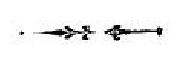
\includegraphics[scale=0.6]{Graphics/Capture3.JPG}\\
~॥~श्रीवरदमूर्तिर्जयति~॥\\
\rule{0.15\linewidth}{0.5pt}\\

\vspace{3mm}
\phantomsection \label{dhanarna}
\underline{धनर्णषड्विधविवरणम्}
\end{center}
 \begin{quote}
     \qt
शिवयोर्भजनातिगौरवोद्य\textendash \\

\vspace{-5mm}
\hspace{0.5cm} त्सुतलीलाधृतकुञ्जरास्यरूपम्~। \\

\vspace{-5mm}
अपहन्तु ममान्तरं तमस्तत् \\

\vspace{-5mm}
\hspace{0.5cm} सततानन्दमयं महो महीयः~॥~१~॥\\

\vspace{-3mm}
यदीयचरणाम्भोजस्मर्तुः सकलसिद्धयः~। \\

\vspace{-5mm}
भवन्ति वशवर्तिन्यः सिद्धेशीं तामहं भजे~॥~२~॥\\

\vspace{-3mm}
मिहिरमिव वराहमिहिरं \\

\vspace{-5mm}
\hspace{0.5cm} वन्दे सन्देहभेदिनं जगताम्~। \\

\vspace{-5mm}
ज्योतिश्चक्रविभावन\textendash \\

\vspace{-5mm}
\hspace{0.5cm} हेतुं जगदेकचक्षुरक्षुद्रम्~॥~३~॥\\

\vspace{-3mm}
कविबुधजनमूर्धनि स्फुरन्तं \\

\vspace{-5mm}
\hspace{0.5cm} कविबुधसन्ततसेवनीयपार्श्वम्~। \\

\vspace{-5mm}
गणितनिपुणतां प्रवर्तयन्तं \\

\vspace{-5mm}
\hspace{0.5cm} प्रणमत भास्करमीप्सितार्थसिद्ध्यै~॥~४~॥ \\

\vspace{-3mm}
कदापि नैव सम्भ्रमः स्थितश्च भौममण्डले~। \\

\vspace{-5mm}
अपूर्वमार्गमाश्रयन् जयत्यपूर्वभास्करः~॥~५~॥\\
 \end{quote}
\afterpage{\fancyhead[RE]{\textbf{बीजपल्लवे}}}
\afterpage{\fancyhead[LO]{\textbf{धनर्णषड्विधविवरणम्}}}
\afterpage{\fancyhead[RO,LE]{\textbf{\thepage}}}
\cfoot{}
\newpage
%%%%%%%%%%%%%%%%%%%%%%%%%%%%%%%%%%%%%%%%%%%%%%%%%%%%%%%%%%%%
\renewcommand{\thepage}{\devanagarinumeral{page}}
\setcounter{page}{2}
\begin{quote}
    \qt
आसीदसीमगुणरत्ननिधानकुम्भः \\

\vspace{-5mm}
\hspace{0.5cm} कुम्भोद्भवाभरणदिग्ललनाललाम~। \\

\vspace{-5mm}
आशैशवार्धितविशेषकलानुवर्ती \\

\vspace{-5mm}
\hspace{0.5cm} श्रीकेशवः सुगणितागमचक्रवर्ती~॥ ६~॥\\

\vspace{-3mm}
तस्मादभूद्भुवनभूषणभूतमूर्तिः \\

\vspace{-5mm}
\hspace{0.5cm} श्रीमानगण्यगुणगौरवगेयकीर्तिः~। \\

\vspace{-5mm}
ज्योतिर्विदागमगुरुर्गुरुसम्प्रदाय\textendash \\

\vspace{-5mm}
\hspace{0.5cm} प्रज्ञानशास्त्रहृदयः सदयो गणेशः~॥ ७~॥\\

\vspace{-3mm}
भ्रातुः सुतस्तस्य यथार्थनामा \\

\vspace{-5mm}
\hspace{0.5cm} नृसिंह इत्यद्भुतरूपशोभः~। \\

\vspace{-5mm}
अवर्धयद्यो जगतामभीष्टं \\

\vspace{-5mm}
\hspace{0.5cm} प्रह्लादमाश्चर्यकरः सुराणाम्~॥~८~॥\\

\vspace{-3mm}
तच्छिष्यो विष्णुनामा स जयति जगती\renewcommand{\thefootnote}{*}\footnote{जगति}जागरूकप्रतिष्ठः \\

\vspace{-5mm}
\hspace{0.5cm} शिष्टानामग्रगण्यः सुभणितगणिताम्नायविद्याशरण्यः~। \\

\vspace{-5mm}
यद्वक्त्रोन्मुक्तमुक्ताफलविमलवचोवीचिमालागलन्तो\textendash \\

\vspace{-5mm}
\hspace{0.5cm} र्द्वित्राः सिद्धान्तलेशा जगति विदधतेऽज्ञेऽपि सर्वज्ञगर्वम्~॥~९~॥\\

\vspace{-3mm}
तस्मादधीत्य विधिवत् त्रिस्कन्धं ज्योतिषं गुरोः~। \\

\vspace{-5mm}
कृष्णो दैवविदां श्रेष्ठस्तनुते बीजपल्लवम्~॥~१०~॥\\

\vspace{-3mm}
अव्यक्तत्वादिदं बीजमित्युक्तं शास्त्रकर्तृभिः~। \\

\vspace{-5mm}
तद्व्यक्तीकरणं शक्यं न विना गुर्वनुग्रहम्~॥~११~॥
\end{quote}
\newpage
%%%%%%%%%%%%%%%%%%%%%%%%%%%%%%%%%%%%%%%%%%%%%%%%%%%
 \onehalfspacing
 अथ शाण्डिल्यगोत्रमुनिवरवंशावतंसजडविडनगरनिवासिकुम्भोद्भवभूषणादिकभूषण-सकलागमचार्यवर्य-\,श्रीमहेश्वरोपाध्यायतनय-निखिलविद्यावाचस्पतिगणितविद्याचतुरानन-धरणितरश्रीभास्कराचार्यः खगणित\renewcommand{\thefootnote}{*}\footnote{स्वगणित}रूपसिद्धान्तशिरोमणिं
चिकीर्षुस्तदुपयोगितया तदध्यायभूतं व्यक्तगणितमुक्त्वा तथाभूतमव्यक्तगणितमारभमाणः 
प्रत्यूहव्यूहनिरासाय शिष्टा-चारपरिपालनार्थं च मङ्गलमाचरन्
शिष्यशिक्षार्थं तदुपजातिकया निबध्नाति\textendash  
\begin{quote}
    \bs
    उत्पादकं यत्त्प्रवदन्ति बुद्धेः \\
    
\vspace{-7mm}
\hspace{1cm} अधिष्ठितं सत्पुरुषेण साङ्ख्याः~। \\
 
\vspace{-7mm}
 व्यक्तस्य कृत्स्नस्य तदेकबीजम् \\
 
\vspace{-7mm}
\hspace{1cm} अव्यक्तमीशं गणितं च वन्दे~॥~१~॥
\end{quote}

 अत्रायमन्वयः~। तदव्यक्तम् ईशं गणितं च वन्दे~। ईशपक्षे 
यत्तदोर्लिंङ्गपरिणामेन यदिति स्थाने यं तदिति स्थाने तं चेति बोद्धव्यम्~।
अव्यक्तं प्रधानम्~। साङ्ख्यशास्त्रे जगत्कारणतया प्रसिद्धम्~। ईशं
सच्चिदानन्दरूपं वेदान्तवेद्यम्~। गणितमत्राव्यक्तमेव~। अव्यक्तपदस्यावृत्त्या 
अव्यक्तं गणितमिति तद्विशेषणस्य विवक्षितत्वात्~। तन्नमस्कारेण च तदधिष्ठात्री देवता नमस्कृता भवति~। शालग्रामशिलादौ तथा दृष्टत्वात्~। तत्र 
प्रधानपक्षे किं तदव्यक्तम्~। साङ्ख्या यद्बुद्धेरूत्पदाकं प्रवदन्ति~।
बुद्धेस्तत्त्वविशेषस्य महदाख्यस्य~। उत्पत्तिरत्राभिव्यक्तिः यतस्ते सत्कार्यवादिनः~॥\\

\vspace{-3mm}
 ननु प्रधानमचेतनं कथं कार्यमुत्पादयेदित्यत उक्तं पुरुषेणाधिष्ठितं 
सदिति~। यथा हि कुलालादिना चेतनेनाधिष्ठितं कपालादि घटाद्युत्पादकं 
तद्वदित्यर्थः~। अत्र साङ्ख्याः सेश्वराः श्रीभगवत्पतञ्जलिमतानुसारिणो
ज्ञेयाः~। निरीश्वरा हि कपिलमुनिमतानुसारिणः पुरुषनिरपेक्षमेव प्रधानमुत्पादकं
प्रवदन्ति~। तदुक्तम् {\qt ईश्वरकृष्णेन सप्तशत्याम्\textendash }

\newpage
%%%%%%%%%%%%%%%%%%%%%%%%%%%%%%%%%%%%%%%%%%%%%%%%%%%
\begin{quote}
    {\qt "वत्स विवृद्धिनिमित्तं क्षीरस्य यथा प्रवृत्तिरज्ञस्य~। \\
पुरुषविमोक्षनिमित्तं तथा प्रवृत्तिः प्रधानस्य~॥"} इति~। 
\end{quote}

 ननु तादृशे प्रधाने किं प्रमाणमित्यत आह\textendash \,कृत्स्नस्य
व्यक्तस्यैकजबीजमिति~। सम-स्तस्य व्यक्ताव्यक्तस्य कार्यजातस्य एकं बीजमुपादानम्~। तथा च वियदादिकार्यजातं सोपादानकं कार्यत्वात् घटवदित्यनुमानं लाघवसहकृतं तत्र
प्रमाणमिति भावः~। नवा ईश्वरेणार्थान्तरता~। तस्य निर्विकारस्य
अपरिणामितयानुपादानत्वात्~। परिणामित्वेऽपि कथमचेतनं चेतनपरिणामः स्यादिति~। एकमिति पुरुषव्यवच्छेदः~। तन्मते पुरुषस्यानुपादानत्वात्~। यतस्ते वदन्ति पुरुषस्तु
पुष्करपलाशवन्निर्लेप इति~। यथा वेदान्तिमते मायाब्रह्मणी द्वे अपि
प्रपञ्चस्योपादाने~। न तद्वदित्यर्थः~॥ \\

\vspace{-3mm}
 अथेशपक्षे~। साङ्ख्याः सम्यक् ख्यायते ज्ञायते आत्मा यया सा 
साङ्ख्या आत्माकारान्तःकरणवृत्तिः सा येषां ते साङ्ख्या आत्मज्ञानिनः 
सत्पुरुषेण विवेकादिसाधनचतुष्टयसम्पत्तिमता~। अधिष्ठितमादरनैरान्तर्याभ्यां
श्रवणादिविषयीकृतं सन्तं यं बुद्धेस्तत्त्वज्ञानस्योत्पादकं प्रवदन्ति~।
ननु तस्याजनकत्वाद्बुद्धिजनकत्वे मानाभाव इत्यत आह~। समस्तस्य व्यक्तस्य 
कार्यजातस्य एकमसाधारणं बीजमुपादानमित्यर्थः~॥ {\qt "यतो वा इमानि 
भूतानि जायन्ते\,"}  इति~। {\qt "तत्सृष्ट्वा तदेवानुप्राविशत्\,"} इति~। 
{\qt "तस्माद्वा एतस्मादात्मन आकाशः सम्भूतः"}  इत्यादिश्रुतयस्तदुपादानत्वे 
प्रमाणमिति भावः~॥ \\

\vspace{-3mm}
 ननु निर्विकारस्यापरिणामितया कथमुत्पादानत्वमिति चेत् सत्यम्~। 
उपादानं द्विविधम्~। परिणममानं विवर्तमानं चेति~। तत्र परिणामिविक्रियावत्~।
यथा मृदादि घटादेः~। विक्रिया शून्यं विवर्तमानम्~। यथा शुक्त्यादि रजतादेः~।
तत्र यद्यपि निर्विकारस्येशस्य परिणाम्युपादनता नोपपद्यते तथापि
विवर्तमानो-
\newpage
%%%%%%%%%%%%%%%%%%%%%%%%%%%%%%%%%%%%%%%%%%%%%%%%%%%

\noindent पादानत्वेन काप्यनुपपत्तिरस्तीत्यलं पल्लवितेन~। मायोपादानत्वपक्षेऽपि
विवर्तमानोपादानत्वस्यात्र विवक्षितत्वादेकमित्युक्तम्~॥ \\

\vspace{-3mm}
 अत्र गणितपक्षे साङ्ख्याः सङ्ख्याविदो गणकाः सत्पुरुषेण स्वरूपयोग्येन 
अधिष्ठितमभ्यस्तं यद्बुद्धेः शिरोमणिवक्ष्यमाणप्रश्नोत्तरार्थादिज्ञानस्य
उत्पादकं प्रवदन्ति~। ननु प्रश्नोत्तरार्थादिज्ञानस्योत्पादकं व्यक्तमेवास्ति~॥ 


\begin{quote}
    {\qt

 "गुणघ्नमूलोनयुतस्य राशेः \\

\vspace{-7mm}
\hspace{1cm} दृष्टस्य युक्तस्य गुणार्धं कृत्वा~। \\

\vspace{-7mm}
 मूलं गुणार्धेन युतं विहीनं \\

\vspace{-7mm}
\hspace{1cm} वर्गीकृतं प्रष्टुरभीष्टराशिः~॥"} \renewcommand{\thefootnote}{*}\footnote{लीलावत्यां दृष्टमूलजातौ करणसूत्रम्.}इत्यादि~॥\\

 \vspace{-5mm}
{\qt "कुज्योनतद्रहतिहृता कृतशक्रनिघ्नो \\

\vspace{-7mm}
\hspace{1cm} कुज्यैव यत्फलपदं पलभा भवेत्सा~॥"} इति~।\renewcommand{\thefootnote}{$\dag$}\footnote{ ग्रहगणिते त्रिप्रश्नाधिकारे श्लोकः ९३. }\\

\vspace{-5mm}
{\qt द्युज्यापक्रमभानुदोर्गुणयुतिः\\
 
 \vspace{-7mm}
\hspace{1cm} तिथ्यु\textendash \,२५\textendash \,द्धताब्ध्या ४ हता \\
 
 \vspace{-7mm}
 स्यादाद्यो युतिवर्गतो यम\textendash \,२\textendash \,गुणात् \\
 
 \vspace{-7mm}
\hspace{1cm} सप्तामरा\textendash \,३३७\textendash \,प्तोनिता~। \\

\vspace{-7mm}
 नागाद्र्यङ्गदिगङ्ककाः ९१०६७८ पदमतः \\
 
 \vspace{-7mm}
\hspace{1cm} तेनाद्य ऊनो भवेत् \\
 
 \vspace{-7mm}
 व्यासार्धेऽष्टगुणाब्धिपावक\textendash \,३४३८\textendash \,मिते \\
 
 \vspace{-7mm}
\hspace{1cm} क्रान्तिज्यकातो रविः~॥"} इत्यादि वा~।\renewcommand{\thefootnote}{$\ddag$}\footnote{ग्रहगणिते त्रिप्रश्नाधिकारे श्लोकः १०१.}
\end{quote}
\newpage
%%%%%%%%%%%%%%%%%%%%%%%%%%%%%%%%%%%%%%%%%%%%%%%%%%%

 यतो यावत्तावदादिवर्णकल्पनानिरपेक्षैर्गुणनभजनादिमार्गैः क्रियमाणं गणितं
व्यक्तम् इत्युच्यते~। तत्कथमुच्यते प्रश्नोत्तरार्थज्ञानरूपाया
बुद्धेरूत्पादकमव्यक्तमिति अत 
आह व्यक्तस्येति~। व्यक्तस्य यावत्तावदादिवर्णकल्पनानिरपेक्षस्य {\qt "गुणघ्नमूलोनयुतस्य राशेः"} इत्याद्यस्य {\qt "द्युज्यापक्रमभानुदोर्गुणयुतिः
तिथ्युद्धताब्ध्याहता"}  इत्याद्यस्य च गणितस्य एकं बीजं मूलमिति यावत्~। {\qt "द्युज्यापक्रम"}  इत्यादिगणितप्रकारस्य वर्णकल्पनामूलत्वादिति भावः~। श्रेयांसि बहुविघ्नानि इत्युक्तत्वान्नमस्कारत्रयम् उचितमेव~। मङ्गलस्य समाप्तिजन-कत्वं विघ्नध्वंसजनकत्वं वा प्रकृतानुपयुक्तत्वाद्ग्रन्थविस्तरभयाच्च मण्यादौ विस्तृतत्वाच्च नेह व्युत्पाद्यते~। तत्तत एव द्रष्टव्यम्~। ईशस्य समस्तकार्यजनकत्वं वदता तत्प्रणामस्य
ग्रन्थ-समाप्तिप्रचयादिरूपं फलं कैमुतिकन्यायेनैव सूचितम्~। यतो यो यदिष्टमनिष्टं वा कर्तुं शक्तः स स्वप्रणतस्य तदिष्टं स्वद्वेष्टुस्तदनिष्टं च विदधाति~। ईशस्तु
सर्वं कर्तुं शक्तः स्वप्रणतस्य सर्वमिष्टं विदध्यात्~। ग्रन्थसमाप्तिप्रचयादिरूपं किमुतेति~। अत्र साङ्ख्यवेदान्तिमतव्युत्पादनं ग्रन्थविस्तरभयान्न कृतं तत्रैवावगन्तव्यम्~॥ \\

\vspace{-3mm}
 इदानीं प्रेक्षावत्प्रवृत्तिहेतुविषयादिचतुष्टयसङ्गतिं च शालिन्या
दर्शयति\textendash 

\phantomsection \label{1.2}
\begin{quote}
    \bs
 पूर्वं प्रोक्तं व्यक्तमव्यक्तबीजं \\

\vspace{-7mm}
\hspace{0.5cm} प्रायः प्रश्ना नो विनाव्यक्तयुक्ता~। \\
 
  \vspace{-7mm}
 ज्ञातुं शक्या मन्दधीभिर्नितान्तं \\

\vspace{-7mm}
\hspace{0.5cm} यस्मात्तस्माद्वच्मि बीजक्रियां च~॥~२~॥
\end{quote}

 अस्यार्थः~। तस्माद्धेतोर्बीजस्य यावत्तावदादि वर्णकल्पनादिभिः क्रियमाणस्य गणितस्य क्रियामिति कर्तव्यतां वच्मि~। यस्मादव्यक्तं
वर्णकल्पनानिरपेक्षं गणितम्~। पूर्वं प्रोक्तं ततः किमित्यत आह~। अव्यक्तबीजमिति~॥ 
अव्यक्तं बीजगणितं बीजं मूलं यस्य~। तथा च पूर्वं प्रोक्तमपि व्यक्तं 
तावत्सम्यक्तया न ज्ञायते यावद्बीजक्रिया नोपपद्यते~। तत्किं
व्यक्तज्ञानार्थ\textendash
\newpage
%%%%%%%%%%%%%%%%%%%%%%%%%%%%%%%%%%%%%%%%%%%%%%%%%%%

\noindent मेवायमारम्भः, नेत्याह~। यस्माच्च सुधीभिरथवाव्यक्तयुक्त्या विना प्रश्ना
ज्ञातुं प्रायो न शक्याः~। मन्दधीभिस्तु नितान्तं ज्ञातुमशक्या एवेत्यर्थः~।
प्रश्नाश्चात्र {\qt सिद्धान्तशिरोमणौ त्रिप्रश्नाधिकारे} वक्ष्यमाणाः\textendash \,{\qt "भाकर्णे खगुणाङ्गुले ३० किल सखे याम्यो भुजस्त्र्यङ्गुलः\renewcommand{\thefootnote}{*}\footnote{ग्रहगणिते त्रिप्रश्नाधिकारे श्लोकः ७५.}"}  इत्यादयः परे प्रश्नाध्यायोक्ता इतरे
पृच्छकेच्छावशादपि ज्ञातव्याः~। यद्वा, तस्माद्व्यक्तं पूर्वं प्रोक्तम् इदानीं
बीजक्रियां च वच्मि~। यस्मादव्यक्तयुक्त्या विना प्रश्नाः प्रायो बहुधा ज्ञातुं नो 
शक्याः~। तेनैवमुपलभ्यते केचन प्रश्ना व्यक्तयुक्त्यापि ज्ञातुं शक्यन्ते~।
वक्ष्यति च {\qt प्रश्नाध्याये\textendash }
\begin{quote}
    {\qt 
     "पाद्या च बीजेन च कुट्टकेन \\

\vspace{-7mm}
\hspace{1cm} वर्गप्रकृत्या च तथोत्तराणि~। \\

\vspace{-7mm}
\hspace{1mm} गोलेन यन्त्रैः कथितानि तेषां \\

\vspace{-7mm}
\hspace{1cm} बालावबोधे कतिचिच्च वच्मि~॥"}\renewcommand{\thefootnote}{$\dag$}\footnote{गोलाध्याये प्रश्नाध्याये श्लो २.} इति~। 

\end{quote}

 तथा च प्रश्नोत्तरार्थज्ञानसाधनं व्यक्तमव्यक्तं च भवति यतस्तस्माद्व्यक्तं पूर्वं प्रोक्तमिदानीं बीजक्रियां च वच्मीत्यर्थः~॥ \\

\vspace{-3mm}
 ननु प्रश्नोत्तरार्थज्ञानसाधनं द्वयम् अपि भवत्यभ्यर्हितं त्वव्यक्तम् एव
तत्कथं व्यक्तं पूर्वं प्रोक्तमित्यत आह~। \hyperref[1.2]{\textbf{अव्यक्तबीजम्}} इति~। अव्यक्तस्य बीजं मूलम्~। तथा च यावत् व्यक्तगणितोक्तभिन्नपरिकर्माष्टकत्रैराशिकादिकं न 
ज्ञायते तावदव्यक्तप्रवेशो न भवतीति व्यक्तं पूर्वं प्रोक्तमिति भावः~। 
तदेवं व्यक्तसापेक्षकतया व्यक्तानन्तरं ग्रहगणितोपयुक्ततया
ग्रहगणितात्प्रागव्यक्तस्यारम्भो युक्त इति सङ्गतिः प्रदर्शिता~। असङ्गतप्रलापो हि
प्रेक्षाव-
\newpage
%%%%%%%%%%%%%%%%%%%%%%%%%%%%%%%%%%%%%%%%%%%%%%%%%%%

\noindent तामनवधेयवचनो भवति~। बीजक्रियां वच्मीति वदता एकवर्णसमीकरणानेकवर्णसमीक-रणमध्यमाहरणभावितरूपभेदचतुष्टयभिन्नं गणितं विषयः प्रदर्शितः तदुपयुक्ततया धनर्ण-षड्विधखषड्विधवर्णषड्विधकरणीषड्विधकुट्टकवर्गप्रकृतिचक्रवालान्यपि विषयत्वेन प्रदर्शितानि~। विषयस्य शास्त्रस्य च
प्रतिपाद्यप्रतिपादकभावः सम्बन्धोऽपि बीजक्रियां वच्मीत्यनेन दर्शितः~। यद्वा ज्ञातेऽपि 
विषये च वेदबाह्यैः\renewcommand{\thefootnote}{*}\footnote{बोध्यैः} हैतुकैराधुनिकैः कल्पितमिदमुत पारम्पर्यागतमिति 
संशयेन नूतनकल्पितमेवेदं शास्त्रमिति भ्रमेण वा प्रेक्षावन्तः शिष्टा न 
प्रवर्तेरन्~। तदर्थं पारम्पर्यलक्षणसम्बन्धकथनमावश्यकम्~। तच्च बीजगणितस्य
प्रश्नज्ञानसाधनत्वं वदता आचार्येण कृतमेव~। तथा हि\textendash \,अव्यक्तगणितं प्रश्नज्ञानसाधनत्वाज्ज्यौतिषम्~। ज्यौतिषत्वाद्वेदाङ्गं
वेदाङ्गत्वाद्ब्रह्मणः सकाशाद्वसिष्ठादिद्वारा पारम्पर्येणागतमित्युक्तं भवति~। उक्तं च नारदेन\textendash \,अस्य शास्त्रस्य सम्बन्धो वेदाङ्गमिति धातृत\textendash \,इति~। आचार्योऽपि {\qt गोलाध्याये} स्पष्टीकृतिवासनायां वक्ष्यति\textendash  
\begin{quote}
    {\qt
\hspace{-3mm} "दिव्यं ज्ञानमतीन्द्रियं यदृषिभिर्ब्राह्मं वसिष्ठादिभिः \\

\vspace{-7mm}
 \hspace{0.6cm} पारम्पर्यवशाद्रहस्यमवनीं नीतं प्रकाश्यं ततः~। \\

\vspace{-7mm}
 \hspace{-1.5mm} नैतद्द्वेषिकृतघ्नदुर्जनदुराचाराचिरावासिनां \\

\vspace{-7mm}
\hspace{0.6cm} स्यादायुः सुकृतक्षयो मुनिकृतां सीमामिमामुज्झतः~॥"} इति~॥\renewcommand{\thefootnote}{$\dag$}\footnote{गोलाध्याये स्फुटगनिवासनाया छेद्याधिकारे श्लोकः ९.}
\end{quote}


 प्रयोजनं तु प्रश्नोत्तरार्थज्ञानम्~। गोलज्ञानं च~। परम्परया जगतः 
शुभाशुभफलादेशश्च~। यतो वक्ष्यति {\qt गोलाध्याये\textendash }
\begin{quote}
    \qt
 "ज्योतिः शास्त्रफलं पुराणगणकैरादेश इत्युच्यते \\

\vspace{-7mm}
\hspace{0.5cm} नूनं लग्नबलाश्रितः पुनरयं तत्स्पष्टखेटाश्रयम्~। \\
\end{quote}
\newpage%%%%%%%%%%%%%%%%%%%%%%%%%%%%%%%%%%%%%%%%%%%%%%%%%%%
\begin{quote}
    {\qt
 ते गोलाश्रयिणोऽन्तरेण गणितं गोलोऽपि न ज्ञायते \\

\vspace{-7mm}
\hspace{0.5cm} तस्माद्यो गणितं न वेत्ति स कथं गोलादिकं ज्ञास्यति~॥"} इति~।\renewcommand{\thefootnote}{*}\footnote{गोलाध्याये गोलप्रशांसाप्रकरणे श्लोकः ६~।}
\end{quote}

{\qt नारदोऽपि\textendash \,"प्रयोजनं तु जगतः शभाशुभनिरूपणम्"} इति~। \\

\vspace{-3mm}
मुख्यं तु शास्त्रप्रयोजनमेवास्य प्रयोजनम्~। 

\begin{quote}
    {\qt
 "यो ज्योतिषं वेत्ति नरः स सम्यक् \\

\vspace{-7mm}
\hspace{0.5cm} धर्मार्थमोक्षाँल्लभते यशश्च~।"} इति~। 
\end{quote}

इहाधिकारी तु प्रश्नादिजिज्ञासुः पठितव्यक्तश्च~। स च द्विज एव~। यद्वक्ष्यति {\qt सिद्धान्तशिरोमणौ\textendash }

\begin{quote}
    {\qt
 "तस्माद्द्विजैरध्ययनीयमेव\renewcommand{\thefootnote}{$\dag$}\footnote{अध्ययनीयमेतत् इति पाठभेदः~। }\\
 
 \vspace{-7mm}
\hspace{0.5cm} पुण्यं रहस्यं परमं च तत्त्वम्~।"} इति~।\renewcommand{\thefootnote}{$\ddag$}\footnote{ग्रहगणिते मध्यमाधिकारे कालमानाध्यायः श्लोकः १२~।}
\end{quote}

 अत्र एवकारस्य पाठक्रमेण योजने ज्यौतिषस्यावश्याध्ययनीयता 
प्रतीयते~। द्विजैरेवेति योजने द्विजातिरिक्तैरनध्ययनीयता च प्रतीयते~। द्वे
अप्यत्र युक्ते इति~। \\

\vspace{-3mm}
 ननु यद्वेति व्याख्याने अव्यक्तबीजमित्यत्र तत्पुरुषसमासे व्यक्तस्य 
कृत्स्नस्य तदेकबीजमिति पूर्वग्रन्थविरोधः~। कश्चिदव्यक्तभागो व्यक्तस्य
बीजं 
कश्चित् व्यक्तभागोऽव्यक्तस्य बीजमिति न विरोध इति चेत् न,
कृत्स्नपदस्योक्तत्वात्~। न च व्यक्तस्य कृत्स्नस्य तदेकबीजमिति बीजस्य व्यक्तमूलकत्वेऽप्यविरुद्धत्वमिति वाच्यम्~। व्यक्तज्ञानेऽव्यक्तज्ञानमव्यक्त-ज्ञाने
च 

\newpage%%%%%%%%%%%%%%%%%%%%%%%%%%%%%%%%%%%%%%%%%%%%%%%%%%%

\noindent व्यक्तज्ञानमिति परस्पराश्रयस्य दुस्तरत्वात्~। मैवम्~। {\qt "गङ्गा गङ्गेति यो ब्रूयाद्योजनानां शतैरपि~। मुच्यते सर्वपापेभ्यः"} इत्यादौ सर्वशब्दस्येव
प्रकृते कृत्स्नशब्दस्य बहुत्वपरत्वात्~। इतरथा
व्यक्तानन्तरमव्यक्तारम्भानुपपत्तेः~। अत एव कश्चन व्यक्तभागोऽव्यक्तमूलं कश्चिदव्यक्तभागो 
व्यक्तमूलमिति विरोधपरिहारो युक्त एव~। कृत्स्नपदे
सङ्कोचस्यावश्याभ्युपेयत्वात्~। न हि व्यक्तोक्तसङ्कलनव्यवकलनादिष्वपि अव्यक्तं मूलमिति 
केनाप्यूरीक्रियते~। किं तु {\qt "गुणघ्नमूलोन"} इत्यादावेव~। किं च 
कृत्स्नपदे सङ्कोचाभावेऽपि न कश्चिद्दोषः~।~तथा हि यथा  {\qt "गुणघ्नमूलोन"} इत्यादि व्यक्तगणितस्याव्यक्तमूलकत्वेऽपि न स्वरूपनिर्वाहाय
तद-पेक्षा किं तूपपत्तावेव तद्वदखिलस्यापि व्यक्तस्याव्यक्तमूलकत्वे कुतः स
परस्पराश्रय इत्यलं पल्लवितेन~॥ \\

\vspace{-3mm}
 अव्यक्तक्रिया तावदव्यक्तषड्विधाधीना, तदपि धनर्णषड्विधाधीनम्, अतः 
प्रथमतस्तदत्र प्रतिपादनीयम्~। तत्रापि व्यवकलनादीनां
सङ्कलनपूर्वकत्वाद्धनर्णसङ्कलनं तावदुपजातिका-पूर्वार्धेनाह\textendash 

\phantomsection \label{1.3.1}
\begin{quote}
    \bs
     योगे युतिः स्यात् क्षययोः स्वयोर्वा \\

\vspace{-7mm}
\hspace{1cm} धनर्णयोरन्तरमेव योगः~। 
\end{quote}

 क्षययोः ऋणयोः स्वयोः धनयोर्वा योगे कर्तव्ये युतिः स्यात्~। एतदुक्तं 
भवति\textendash \,ययोर्योगः कर्तव्योऽस्ति तौ रूपात्मकौ वर्णात्मकौ
करण्यात्मकौ वा राशी यद्युभावपि ऋणगतौ धनगतौ वा भवतस्तदा तयोः राश्योः कार्यः क्रमादुत्क्रमतोऽथवाङ्कयोग इति व्यक्तगणितोक्तो योगो विधेयः~। स एवात्र योगो भवति~। करण्योस्तु योगोऽन्तरं वा \hyperref[1.12.1]{\textbf{"योगं करण्योर्महती प्रकल्प्या"}} 
इत्यादिवक्ष्यमाणप्रकारेण विधेयमिति द्रष्टव्यम्~। एवं बहूनामपि~। एवं सजातीययोग 
उक्तः~। यत्र त्वेको राशिर्धनमितरश्चर्णं तयोर्योगे कर्तव्ये किं कर्तव्यं
तदाह\textendash \,\hyperref[1.3.1]{\textbf{"धनर्णयोरन्तरमेव योग"}} इति~। व्यक्तरीत्या यदन्तरं सम्पद्यते स एव धनर्णयोर्योग इत्यर्थः~। शेषस्य धनर्णत्ववशाद्योगस्यापि धनर्णत्वं ज्ञेयम्~।
\newpage
%%%%%%%%%%%%%%%%%%%%%%%%%%%%%%%%%%%%%%%%%%%%%%%%%%%

 अथोक्तेऽर्थे शिष्यबोधार्थमुदाहरणचतुष्टयमुपजातिकयाह\textendash 
\begin{quote}
    \ex
 रूपत्रयं रूपचतुष्टयं च \\

\vspace{-7mm}
\hspace{1cm} क्षयं धनं वा सहितं वदाशु~। \\

 \vspace{-7mm}
 स्वर्णे क्षयः स्वं च पृथक् पृथङ्मे \\

\vspace{-7mm}
\hspace{1cm} धनर्णयोः सङ्कलनामवैषि~॥~१~॥
\end{quote}
 
 रूपत्रयं रूपचतुष्टयं चेति द्वयमप्यृणमित्येकं, द्वयमपि धनमिति द्वितीयं,
आद्यं धनमपरमृणमिति तृतीयं, प्रथममृणमितरद्धनमिति चतुर्थम्, एवं 
चत्वार्युदाहरणानि~। धनर्णयोरिति~। धने च ऋणे च धनर्णे~। धनं 
च ऋणं च धनर्णं, धनर्णं च धनर्णं च धनर्णे~। तयोर्धनर्णयोः, 
धनयोः ~ऋणयोः ~धनर्णयोश्चेत्यर्थः~। चतुर्थप्रश्नस्य ~तृतीयेऽन्तर्भूतत्वात् पक्षत्रयमेवोद्दिष्टमिति~॥ \\

\vspace{-3mm}
 नन्विदं धनम् इदम् ऋणमिति वा इदं व्यक्तं इदम् अव्यक्तमित्यादि 
वा कथमवधेयमित्यत आह\textendash \\

\vspace{-3mm}
 अत्र रूपाणामव्यक्तानां चाद्याक्षराण्युपलक्षणार्थमालेख्यानि तथा यानि 
ऋणगतानि तान्यूर्ध्व बिन्दूनि चेति~। अतिरोहितार्थमिदम्~।
यद्यृणत्वादिकमालापत एव अवगन्तुं शक्यम्~। तथाप्यालापबहुत्वे ऋणत्वादौ भ्रान्तिः 
संशीतिर्वा स्यादुपस्थितिलाघवं च न स्यादित्यूर्ध्वबिन्द्वादिलेखनं
युक्ततरम्~। धनर्णत्वं तु व्यवकलनोपपत्तौ विवरिष्यामः~। अत्र प्रथमोदाहरणे न्यासः 
$\dot{\text{३}}$~। $\dot{\text{४}}$ योगे जातं ७ं~। द्वितीये न्यासः ३~। ४~। योगे जातं ७~। तृतीये न्यासः ३~। $\dot{\text{४}}$~। \hyperref[1.3.1]{\textbf{"धनर्णयोरन्तरमेव योगः"}} इति जातम् $\dot{\text{१}}$~। चतुर्थे न्यासः ४~। $\dot{\text{३}}$~। \hyperref[1.3.1]{\textbf{"अन्तरमेव योगः"}} इति जातम् १~। अत्रोपपत्तिर्लोकसिद्धैव~। तथाहि\textendash \,देवदत्तस्य मुद्रात्रयमृणमेकमितरदपि मुद्राचतुष्टयमृणमित्यभिहिते मुद्रासप्तकमृणमस्तीति प्रतीतिरस्त्यागोपालाविपालेभ्यो व्यवहारसिद्धा~॥
\newpage
%%%%%%%%%%%%%%%%%%%%%%%%%%%%%%%%%%%%%%%%%%%%%%%%%%%

 एवं देवदत्तस्य मुद्रात्रयमेकं धनमन्यदपि मुद्राचतुष्टयं धनमस्तीत्युक्ते
अस्त्यस्य मुद्रासप्तकं धनमिति विलसति सार्वजनीनो व्यवहारः~। अत उक्तम् 
\hyperref[1.3.1]{\textbf{"योगे युतिः स्यात् क्षययोः स्वयोर्वा"}} इति~॥\\

\vspace{-3mm}
 अथ देवदत्तस्य मुद्रात्रयं धनमस्ति मुद्राचतुष्टयमृणमप्यस्तीत्युक्ते 
नास्य धनमस्ति किं तूत्तमर्णस्य मुद्रात्रये दत्ते एकैव
मुद्रास्यर्णमस्तीति वरीवर्ति सकलजनसाधारणो व्यवहारः~। एवं देवदत्तस्य मुद्रात्रयमृणं
मुद्राचतुष्टयं धनमप्यस्तीत्यभिहिते नास्त्यस्यर्णं किं तु
मुद्रैकाधनमस्तीत्यस्ति सकललोकसम्प्रतिपन्नो व्यवहारः~। अत उक्तम् \hyperref[1.3.1]{\textbf{"धनर्णयोरन्तरमेव योगः"}} इति~॥ \\

\vspace{-3mm}
 ननु व्यक्ते भिन्नानामभिन्नानां च सङ्कलनव्यवकलनादि पृथक् पृथगुक्तम्~। 
अत्र तु भिन्नानां सङ्कलनं व्यवकलनाद्यं च न पृथगभिहितमस्ति~। 
तत्कथं कर्तव्यमिति तदाह\textendash \,एवं भिन्नेष्वपीति~। अथायमर्थः~।
सछेदानामपि रूपाणां वर्णानां वा योगार्थं धनर्णत्ववशाद्योगेऽन्तरे वा प्राप्ते
{\qt "योगोऽन्तरं तुल्यहरांशकानाम्"} इत्यादिना योगोऽन्तरं वा विधेयमिति~। एवं
भिन्नव्यवकलनादिष्वपि बोद्धव्यम्~॥\ldots.\ldots.~॥ यथा व्यवकलनादीनां सङ्कलनोपजीवकत्वात्तत्प्राथम्येन सङ्कलननिरूपणं युक्तं न तथा गुणनप्राथम्येन
व्यवकलननिरूपणं युक्तम्, उपजीव्योपजीवकभावाभावात्तथापि
धनर्णताव्यत्यासमात्रविलक्षणस्य 
व्यवकलनस्य गुणनापेक्षया सङ्कलनान्तरङ्गत्वात् खण्डगुण {\qt "इष्टेन युक्तेन गुणेन निघ्न"} इत्यस्मिन्नपि गुणने तस्योपजीव्यत्वाच्च गुणनप्राथम्येन
तन्निरूपणं युक्तमिति उपजातिकोत्तरार्धेन तदाह\textendash  

\phantomsection \label{1.3}
\begin{quote}
    \bs
     संशोध्यमानं स्वमृणत्वमेति \\
  
  \vspace{-7mm}
\hspace{1cm} स्वत्वं क्षयस्तद्युतिरुक्तवच्च~॥~३~॥

\end{quote}

 संशोध्यते अपनीयते तत्संशोध्यमानम्~। रूपवर्णाः करणी वेति 
त्रिलिङ्गसामान्यात् नपुंसकत्वम्~। तद्यदि धनमस्ति तर्हि ऋणत्वमेति~। यदि

\newpage
%%%%%%%%%%%%%%%%%%%%%%%%%%%%%%%%%%%%%%%%%%%%%%%%%%%

\noindent क्षयोऽस्ति तर्हि धनत्वमेति~। पश्चादुक्तवत्तद्युतिश्च~। एतदुक्तं भवति\textendash \,ययोरन्तरं विधेयमस्ति तयोर्मध्ये संशोध्यमानस्य धनर्णता व्यत्यासं कृत्वा \hyperref[1.3.1]{\textbf{"योगे युतिः स्यात्~।"}} इत्यादिना तयोर्युतिः कर्तव्या~। तदेव व्यवकलनफलं भवतीत्यर्थः~। अत्रोपपत्तिः~। ऋणत्वमिह त्रिधा तावदस्ति\textendash \,देशतः, कालतः, वस्तुतश्चेति~। तच्च वैपरीत्यमेव~। यत उक्तमाचार्यै{\qt र्लीलावत्यां क्षेत्रव्यवहारे "दशसप्तदशप्रमौ भुजौ\renewcommand{\thefootnote}{*}\footnote{लीलावत्यां क्षेत्रव्यवहारे ऋणाबाधोदाहरणं श्लोकः १५~।}"} इत्यस्मिन्नुदाहरणे~। ऋणगता आबाधा दिग्वैपरीत्येनेत्यर्थ इति~। तत्रैकरेखा स्थिता द्वितीया दिक् विपरीता दिगित्युच्यते~। 
यथा पूर्वविपरीता पश्चिमा दिक्~। यथा वोत्तरदिग्विपरीता दक्षिणा दिगित्यादि~। तथा च पूर्वापरदेशयोर्मध्ये एकतरस्य धनत्वे कल्पिते तं प्रति तदितरस्य ऋणत्वम्~। यथा पूर्वगतेर्धनत्वकल्पने यदा ग्रहः पश्चिमगतिर्भवति तदा ग्रहे गतितुल्यकला ऋणं भवति~। यथा वा पश्चिमभ्रमस्य धनत्वे यावद्ग्रहः पूर्वतो गच्छति तावत्पश्चिमभ्रमे ऋणमिति दक्षिणोत्तरदेशादिष्वप्येवमेव धनर्णत्वं बोध्यम्~। एवं पूर्वोत्तरकालयोरन्योन्यम् ऋणत्वं वारप्रवृत्त्यादिषु प्रसिद्धम्~॥ \\

\vspace{-3mm}
 एवं यस्मिन् वस्तुनि यस्य स्वस्वामिभावः सम्बन्धः तस्य तद्धनमिति 
व्यवह्नियते~। तस्मिन् वैपरीत्यं तु परस्य स्वस्वामिभावः सम्बन्धः~। अतो 
देवदत्तस्वामिके धने यावति यज्ञदत्तस्वामिकत्वं तावद्देवदत्तस्यर्णमिति
व्यवह्रियते~। तत्र पूर्वदेशस्य धनत्वं पश्चिमदे-शस्य च ऋणत्वं प्रकल्प्योपपत्तिरुच्यते~।
सा यथा\textendash \,श्रीविश्वेशितुः शम्भोः आनन्दकाननात् पुरन्दरदिशि पञ्चदशसु योजनेषु स्वर्गतरङ्गिणीतीरविलासी वरीवर्ति किलैकं पत्तनम्~। वरुणदिशि वा अष्टसु योजनेषु इन्दीवरदलश्यामलपतङ्गतनयान्तरङ्गचुम्बिभिः शरच्चन्द्रिकाधवलैः सुरनदीलोलकल्लोलैः स्मृतहरिहरमूर्तिरानन्दलहरीरनुभवन् जागर्ति तीर्थराजः प्रयागः~। तयोस्तूच्चावचसकलजनव्यवहारसिद्धमस्ति त्रयोविंशतियोजनात्मकमन्तरम्~। तच्च योगं 
\newpage
%%%%%%%%%%%%%%%%%%%%%%%%%%%%%%%%%%%%%%%%%%%%%%%%%%%

\noindent विना नोपपद्यते~। अतो विजातीययोरन्तरे साध्ये योगः कर्तव्यः~। परं स योगः पश्चिमः पूर्वो वा~। तत्र पत्तनात्प्रयागः कस्यां दिशीति विचारे
तावदानन्दकाननात् प्रयागपर्यन्तम् अष्टयोजनात्मको देशः यथा पश्चिमः तथा पत्तनादपि पश्चिमो भवति~। किं त्वानन्दकाननात् पत्तनपर्यन्तं पञ्चदशयोजनात्मको यः पूर्वदेशः
स भवति पत्तनात् पश्चिम एव~। एवं पत्तनात् प्रयागपर्यन्तं देशविचारे
आनन्दवनपर्यन्तं पञ्चदशयोजनात्मकमेकं शकलं ततः प्रयागावधि
द्वितीयमष्टयोजनात्मकम्~। शकलद्वयस्य पश्चिमत्वाज्जातस्त्रयोविंशतियोजनात्मकः पश्चिमो देशः~। एवं प्रयागात् पत्तनं कस्यां दिशीति विचारे प्रयागादानन्दवनपर्यन्तं
देशशकलं विपरीतदिक्त्वं भवति~। तथा च यस्मादनन्तरं साध्यते तदवधिशकलं 
विप-रीतदिक्त्वं भवतीत्यत उक्तम् \hyperref[1.3]{\textbf{"संशोध्यमानं स्वमृणत्वमेति स्वत्वं क्षयः"}} इति~। एवं धनर्णयोरन्तरे प्रतिपादितम्~। एवं धनयोरपि तद्यथा एकः किल काशीतः पूर्वदिग्भागे दशयोजनानि गत इतरोऽपि तस्मिन्नेव भागे सप्तयोजनानि गतः तयोश्चान्तरं योजनत्रयं सर्वजनसिद्धम्~। तच्च दशयोजनगात् पश्चिमम्~। सप्तयोजनगात् पूर्वम्~। इदमपि प्रथमावधिभूतस्य खण्डस्य व्यत्यासे कृते धनर्णयोरन्तरमेव योग इति योगे च कृते सिध्यति~। एवमृणयोरपि बोध्यम्~। अत उपपन्नम् \hyperref[1.3]{\textbf{"संशोध्यमानं स्वमृणत्वमेति स्वत्वं क्षयस्तद्युतिरुक्तवच्च"}} इति~। \\

\vspace{-3mm}
 अन्यदपि सुधीभिरूहनीयम्~। अत्रोदाहरणचतुष्टयम् उपजातिकापूर्वार्धेनाह~। 
\begin{quote}
    \ex
     त्रयात् द्वयं स्यात् स्वमृणादृणं च \\
 
 \vspace{-7mm}
\hspace{1cm} व्यस्तं च संशोध्य वदाशु शेषम्~। 
\end{quote}

 स्वात् त्र्याद्द्वयं स्वमित्येकमृणात् त्रयादृणं द्वयमित्युदाहरणद्वयम्~।
व्यस्तत्वे च स्वात् त्रयादृणं द्वयमित्येकमृणात्त्रयात्स्वं द्वयमिति दितीयमेवं
चत्वार्युदाहरणानि~। तत्र प्रथमे न्यासः ३~। २~। संशोध्यमानं २ स्वमृणत्वमेतीति जातम् ३~। $\dot{\text{२}}$~। अनयोर्युतिरुक्तवत्~। \hyperref[1.3.1]{\textbf{"धनर्णयोरन्तरमेव योगः"}} इति जातम् १~। द्वितीये
\newpage
%%%%%%%%%%%%%%%%%%%%%%%%%%%%%%%%%%%%%%%%%%%%%%%%%%%

\noindent न्यासः  $\dot{\text{३}}$~। $\dot{\text{२}}$~। जातमुक्तवदन्तरम् $\dot{\text{१}}$~। तृतीये न्यासः ३~।
$\dot{\text{२}}$~। {\qt "संशोध्यमानं क्षयः स्वत्वमेति"} इत्यादिना जातम् ५~। चतुर्थे न्यासः $\dot{\text{३}}$~। २~। \hyperref[1.3]{\textbf{"संशोध्यमानं स्वमृणत्वमेति"}} इत्यादिना जातम् $\dot{\text{५}}$~। इदमेव प्रतीत्यर्थं पूर्वपश्चिमदेशत्वेन योज्यते~। पू३पू२-संशोध्यमानः पूर्वदेशः पश्चिमदेशो भवतीति जातम् पू३ प२~। अनयोर्धनर्णयोरन्तरम् एव योग इति शेषम् अन्तरम् पू१~। अत्रैकस्मादवधेः पूर्वतो योजनद्वयेन त्रयेण च नरौ तिष्ठतः~। तत्र योजनद्वयगतात् योजनत्रयगो योजनम् एकं पूर्वतस्तिष्ठतीत्यर्थः~। अत्रोदाहरणेषु द्वयस्य शोध्यतोक्तेर्योजनद्वयगान्नरादन्तरं ज्ञातव्यम्~। अथ द्वितीये प३प२~। उक्तवदन्तरे जातं प१~। पश्चिमतो योजनत्रयगतः पश्चिमतो योजनद्वयगतादेकेन योजनेन पश्चिमतस्तिष्ठतीत्यर्थः~। तृतीये न्यासः पू३प२ उक्तवदन्तरे जातं पू५~। पश्चिमतो योजनद्वयगतात् सः पूर्वतो \;योजनत्रयगः पू५ पञ्चभिर्योजनैः \;पूर्वतस्तिष्ठतीत्यर्थः~। चतुर्थे \;न्यासः प३पू२~। उक्तवज्जातम् अन्तरं प५~। पूर्वतो योजनद्वयगतात् पश्चिमतो योजनत्रयगः पञ्चभिर्योजनैः पश्चिमतस्तिष्ठतीत्यर्थः~॥ \\

\vspace{-3mm}
 अथ भागहारादीनां गुणतोपजीवकत्वाद्भुजङ्गप्रयातपूर्वार्धखण्डेन गुणनमाह\textendash 

\phantomsection \label{1.4.1}
\begin{quote}
    \bs स्वयोरस्वयोः स्वं वधः स्वर्णघाते क्षयः~। 
\end{quote}

 स्वयोरस्वयोर्वा वधो गुणनम्~। एकस्यापरतुल्या आवृत्तिरिति यावत्~। धनं 
भवति~। स्वर्णघाते तु क्षयो भवति~। एतदुक्तं भवति\textendash \,यदा गुण्यो
गुणकश्चेति द्वावपि धनमृणं वा भवतस्तदा तदुत्थं गुणनफलं धनं भवति इति~। अत्र 
गुणनफलस्य धनर्णत्वमात्रं प्रतिपादितम् अङ्कतस्तु व्यक्तोक्ताः सर्वेऽपि
गुणनप्रकारा द्रष्टव्याः~॥ \\

\vspace{-3mm}
 अथ गुणनोदाहरणत्रयमुपजातिकोत्तरार्धेनाह\textendash  
\begin{quote}
    \ex
 धनं धनेनर्णमृणेन निघ्नं \\

\vspace{-7mm}
\hspace{1cm} द्वयं त्रयेण स्वमृणेन किं स्यात्~॥~२~॥
\end{quote}

 स्पष्टोऽर्थः~। ऋणं धनेनेति~। चतुर्थमप्युदाहरणं द्रष्टव्यम्~। अत्र गुणकः ३
गुण्यः २~। अथ प्रथमे न्यासः २~। ३~। उक्तवज्जातं गुणनफलं धनम् ६~। द्वितीये
\newpage%%%%%%%%%%%%%%%%%%%%%%%%%%%%%%%%%%%%%%%%%%%%%%%%%%%

\noindent न्यासः $\dot{\text{२}}$~। $\dot{\text{३}}$~। \hyperref[1.4.1]{\textbf{"अस्वयोर्वधः स्वम्"}} इति जातम् ६~। तृतीये न्यासः २~। $\dot{\text{३}}$~। {\qt "स्वर्णघाते क्षयः"} इति जातम् $\dot{\text{६}}$~। चतुर्थे न्यासः $\dot{\text{२}}$~। ३ \hyperref[1.4.1]{\textbf{"स्वर्णघाते क्षयः"}} इति $\dot{\text{६}}$~। गुण्येन हते गुणे च तदेवेति कर्णिकया गुण्यत्वगुणकत्वयोः कामचारः प्रदर्शितः~॥ \\

\vspace{-3mm}
 ननु स्वयोर्वधः स्वं भवतु नाम सजातीयत्वाद्दृष्टचरत्वाच्चापरम् ऋणयोर्वधः 
कथं धनं भवतु विजातीयत्वात्~। एवं स्वर्णघातेऽपि क्षयः कथं 
भवतु~। न च विजातीयत्वादिति वाच्यम्~। वैपरीत्यस्यापि सुवचत्वाद्धनमेव 
कथं न स्यात् विनिगमनाविरहात्~। अत्रोच्यते~। गुण्यस्य गुणकतुल्या 
आवृत्तिर्हि गुणनफलमिति तावत् प्रसिद्धम्~। तत्र गुणको द्विविधः \;धनमृणं 
चेति~। तत्र \;धनगुणके सति \;धनस्य ऋणस्य वा \;गुण्यस्य आवर्तने 
क्रियमाणे क्रमेण धनम् ऋणं च गुणनफलं स्यात्~। अतः स्वयोर्वधः 
स्वं गुणकस्य धनत्वे गुण्यस्यर्णत्वे ऋणमिति सिद्धम्~॥ \\

\vspace{-3mm}
 अथर्णगुणके विचारः~। तत्रर्णत्वं वैपरीत्यम् इति प्रागेव प्रतिपादितम्~। 
तथा च ऋणगुणको नाम विपरीतगुणकः~। गुण्यस्य विपरीतावर्त्तनकर इति 
यावत्~। तथा सति धने गुण्ये गुणनफलमृणम्~। ऋणे गुण्ये गुणनफलं धनमिति सिद्धम्~। अत्र अन्तिमपक्षेऽस्वयोर्वधः स्वमित्युपपन्नम्~। 
मध्यपक्षयोस्तु गुण्यगुणकयोरेकतरस्य धनत्वेऽन्यस्यर्णत्वे फलमृणमुत्पद्यत
इति स्वर्णघाते क्षय इत्युक्तम्~। यद्वा गणितेनोपपत्तिः प्रदर्श्यते~। धनगुणने
तावदविवाद एव~। ऋणगुणने तु विचारः~। अस्ति तावदिदं सुप्रसिद्धम्~। 
गुण्यो गुणको खण्डाभ्यां पृथग्गुणितः सहितश्च गुणनफलं भवतीति~। 
तथा गुण्यः १३५~। गुणकः १२~। अस्य खण्डद्वयं ४~। ८~। एकमिष्टम् इष्टोनो 
राशिरपरं च~। खण्डाभ्यां पृथग्गुणितो गुण्यः ५४०~। १०८०~। योगे जातं 
गुणनफलं १६२०~। एवमेव कल्पितमिष्टम् $\dot{\text{४}}$~। एतदूनो राशिः १२ द्वितीयखण्डम् १६~। अत्रापि पृथक्खण्डद्वयगुणितेन सहितेन च गुण्येन गुणनफले भवितव्यम्~। तत्र खण्डाभ्यां $\dot{\text{४}}$~। १६~। पृथग्गुणितो गुणः ५४०~। २१६०~। अनयोर्योगे
\newpage
%%%%%%%%%%%%%%%%%%%%%%%%%%%%%%%%%%%%%%%%%%%%%%%%%%%

\noindent गुणनफलं नोपपद्यत इति गुणनफलान्यथानुपपत्त्या \hyperref[1.4.1]{\textbf{"स्वर्णघाते क्षयो भवति"}} इत्यवगम्यते~। यतस्तथा कृते $\dot{\text{५४०}}$~। २१६०~। \hyperref[1.3.1]{\textbf{"धनर्णयोरन्तरमेव योगः"}} इति १६२० गुणनफलमुपपद्यते~। अत उक्तम् \hyperref[1.4.1]{\textbf{"स्वर्णघाते क्षयः"}}~। एवं गुण्यखण्डे प्रत्येकं गुणखण्डगुणिते सहिते च गुणनफलं भवति तद्यथा गुण्यः १३५~। एतस्य खण्डद्वयं १३०~। ५~। गुणकस्यापि १२ खण्डद्वयं ४~। ८~। गुणकखण्डाभ्यां प्रत्येकं गुणितं गुण्यपूर्वखण्डं १३० जातम् ५२०~। १०४०~। \\

\vspace{-3mm}
 एवमेव प्रत्येकं गुणितं द्वितीयखण्डं ५ जातम् २०~। ४०~। सर्वेषां 
योगे जातं गुणनफलम् १६२०~। एवमेव कृतमभीष्टं खण्डद्वयं गुण्यस्य 
१४०~। $\dot{\text{५}}$~। गुणकस्यापि १६~। $\dot{\text{४}}$~। अत्रापि गुणखण्डाभ्यां प्रत्येकं गुणितं पूर्वखण्डं १४० जातम् २२४०~। $\dot{\text{५६०}}$~। अनयोर्योगः १६८०~। एवमेव 
द्वितीयमपि गुणखण्डाभ्यां पृथग्गुणितम् $\dot{\text{८०}}$~। $\dot{\text{२०}}$~। अत्रर्णगुणितमृणं सजातीयत्वादृणमेवेति कृते गुणनफलं १५८० नोपपद्यत इति गुणनफलान्यथानुपपत्त्या ऋणमृणगुणितं धनं भवतीत्यवगम्यते~। यतस्तथा कृते $\dot{\text{८०}}$~। २०~। गुणनफलं १६२० उपपद्यत इत्यत उक्तम् \hyperref[1.4.1]{\textbf{"अस्वयोर्वधः स्वम्"}} इति~। एवं बुद्धिमद्भिरन्यदप्यूह्यम्~। ननु वर्गस्य समद्विघातरूपतया
गुणनान्तरङ्गत्वाद्भजनानपेक्षत्वाच्च प्रथमतो निरूपणं युक्तम्~। न च भक्तो
गुणः शुध्यतीत्यादिना गुणनप्रकारेण वर्गकरणे भजनस्योपजीव्यतया तस्यैव
प्राथम्येन निरूपणं युक्तमिति वाच्यम्~। गुणनादपि पूर्वं तन्निरूपणप्रसङ्गादिति चेत्
न~। वर्गकरणप्रकाराणामतिविलक्षणतया वर्गस्य गणनं प्रति बहिरङ्गत्वात्, 
प्रत्युत वर्गं प्रति पदस्येव गुणनं प्रति भजनस्यैवान्तरङ्गत्वाद्वर्गं प्रत्युपजीव्यत्वात् प्रथमतस्तन्निरूपणस्यैवावश्यकत्वात्~। कस्यचिद्गुणनप्रकारस्य भजनसापेक्षत्वेऽपि भजननिरपेक्षतयापि गुणनस्य सिद्धत्वाद्भजनस्य तु सर्वथापि गुणनसापेक्षत्वाद्गुणनानन्तरमेव तन्निरूपणं युक्तम् इति भुजङ्गप्रयातपूर्वार्धस्य शेषशकलेनैतदाह\textendash  

\newpage
%%%%%%%%%%%%%%%%%%%%%%%%%%%%%%%%%%%%%%%%%%%%%%%%%%%
\phantomsection \label{1.4.2}
\begin{quote}
    \bs भागहारेऽपि चैवं निरुक्तम्~। 
\end{quote}
 
 भागहारेऽपि गुणनवदेव निरुक्तमित्यर्थः~। एतदुक्तं
भवति\textendash~भाज्यभाजकयोरुभयोरपि धनत्वे ऋणत्वे वा लब्धिर्धनमेव~। यदा त्वेकतरस्य धनत्वम् ऋणत्वमितरस्य तदालब्धमृणमेवेति~। अत्राप्यङ्कतो भागप्रकारो व्यक्तोक्तो ज्ञेयः~। अत्रोदाहरणचतुष्टयमुपजातिकयाह\textendash

\begin{quote}
    \ex
 रूपाष्टकं रूपचतुष्टयेन \\

\vspace{-7mm}
\hspace{1cm} धनं धनेनर्णमृणेन भक्तम्~। \\

 \vspace{-7mm}
 ऋणं धनेन स्वमृणेन किं स्यात् \\

\vspace{-7mm}
\hspace{1cm} द्रुतं वदेदं यदि बोबुधीषि~॥~३~॥
\end{quote}

स्पष्टोऽर्थः~॥ प्रथमे न्यासः
$\begin{matrix}
\vspace{-2mm}
\mbox{८~।}\\
\vspace{-1.5mm}
\mbox{४~।}
\vspace{1mm}
\end{matrix}$ स्वयोर्भागहारः स्वमिति जाता लब्धिर्धनं २~। द्वितीये न्यासः $\begin{matrix}
\vspace{-1mm}
\mbox{$\dot{\text{८}}$~।}\\
\vspace{-1.5mm}
\mbox{$\dot{\text{४}}$~।}
\vspace{1mm}
\end{matrix}$ अस्वयोर्भागहारः स्वमिति जाता लब्धिर्धनमेव २~। तृतीये न्यासः $\begin{matrix}
\vspace{-2mm}
\mbox{$\dot{\text{८}}$~।}\\
\vspace{-1.5mm}
\mbox{४~।}
\vspace{1mm}
\end{matrix}$ स्वर्णभागहरे क्षय इति जाता लब्धिः ऋणं $\dot{\text{२}}$~। चतुर्थे न्यासः $\begin{matrix}
\vspace{-1mm}
\mbox{८~।}\\
\vspace{-1.5mm}
\mbox{$\dot{\text{४}}$~।}
\vspace{1mm}
\end{matrix}$ स्वर्णभागहारे क्षय इति जाता लब्धिः ऋणम् $\dot{\text{२}}$~। अत्रोपपत्तिः~। {\qt "भाज्याद्धरः शुध्यति यद्गुणाः स्यादन्त्यात्फलं तत्खलु भागहारे"} इत्युक्तत्वाद्यस्मिन्नङ्के हरगुणिते भाज्यादपनीते शुद्धिर्भवतीति सा किल लब्धिः तत्र प्रथमे $\begin{matrix}
\vspace{-2mm}
\mbox{८}\\
\vspace{-1.5mm}
\mbox{४}
\vspace{1mm}
\end{matrix}$ धनेन द्वयेन हरे ४ गुणिते ८ भाज्यात् ८ अस्मादपनीते शुद्धिर्भवतीति धनं द्वयं लब्धिः २~। द्वितीयेऽपि $\begin{matrix}
\vspace{-1mm}
\mbox{$\dot{\text{८}}$}\\
\vspace{-1.5mm}
\mbox{$\dot{\text{४}}$}
\vspace{1mm}
\end{matrix}$ धनद्वयेन हरे $\dot{\text{४}}$ अस्मिन् गुणिते $\dot{\text{८}}$ भाज्यादस्मात् $\dot{\text{८}}$ अपनीयमाने संशोध्यमानं क्षयः स्वत्वमेतीति \hyperref[1.3.1]{\textbf{"धनर्णयोरन्तरमेव योगः"}} इति च कृते शुद्धिर्भवतीति द्वयं धनमेव लब्धिः १~। एवं सिद्धं स्वयोर-

\newpage
%%%%%%%%%%%%%%%%%%%%%%%%%%%%%%%%%%%%%%%%%%%%%%%%%%%

\noindent स्वयोर्वा भागहारे स्वमिति~। तृतीये तु $\begin{matrix}
\vspace{-2mm}
\mbox{$\dot{\text{८}}$}\\
\vspace{-1.5mm}
\mbox{४}
\vspace{1mm}
\end{matrix}$ धनद्वयेन हरे ४ गुणिते ८ भाज्यात् $\dot{\text{८}}$ अस्मादपनीते \hyperref[1.3]{\textbf{'संशोध्यमानं स्वमृणत्वमेति'}} इति ऋणयोर्योगे $\dot{\text{१६}}$ शुद्धिर्न स्यादृणगुणिते तु हरे $\dot{\text{८}}$ शुद्धिर्भवतीति ऋणं द्वयं लब्धिः $\dot{\text{२}}$~। एवं चतुर्थेऽपि $\begin{matrix}
\vspace{-1mm}
\mbox{८}\\
\vspace{-1.5mm}
\mbox{$\dot{\text{४}}$}
\vspace{1mm}
\end{matrix}$ ऋणगुणित एव हरः शुध्यतीत्यृणमेव लब्धिरिति सिद्धं स्वर्णभागहारे क्षय इति~। अत उक्तम् \hyperref[1.4.2]{\textbf{"भागहारेऽपि चैवं निरुक्तम्"}} इति~। एवं सकलवर्गोपयुक्तमुक्त्वा वर्गं तन्मूलं च भुजङ्गप्रयातोत्तरार्धेनाह\textendash 

\phantomsection \label{1.4}
\begin{quote}
    \bs
    कृतिः स्वर्णयोः स्वं स्वमूले धनर्णे \\

\vspace{-7mm}
\hspace{1cm} न मूलं क्षयस्यास्ति तस्याकृतित्वात्~॥~४~॥
\end{quote}

 स्वस्य \;ऋणस्य \;वा वर्गः \;स्वं भवति~। अङ्कतस्तु \;वर्गप्रकारा \;व्यक्तोक्ताः \;सर्वेऽपि द्रष्टव्याः~॥ \\

\vspace{-3mm}
 अथ मूलमाह\textendash \,\hyperref[1.4]{\textbf{'स्वमूले धनर्णे'}} इति~। स्वस्य धनस्य मूले धनर्णे स्याताम्~। धनस्यैव वर्गस्य ऋणमपि मूलं भवतीत्यर्थः~। अथात्र विशेषमाह न मूलं क्षयस्यास्तीति~। तत्र हेतुमाह\textendash \,तस्याकृतित्वादिति~। वर्गस्य हि मूलं लभ्यते~। ऋणाङ्कस्तु न वर्गः, कथमतस्तस्य मूलं लभ्यते~। ननु ऋणाङ्कः कुतो वर्गो न भवति, न हि राजनिर्देशः~। किं च यदि न वर्गास्तर्हि तस्य वर्गत्वं निषेद्धुमप्यनुचितमप्रसक्तेः सत्यम्~। ऋणाङ्कं वर्गं वदता भवता कस्य स वर्ग इति वक्तव्यम्~। न तावद्धनाङ्कस्य, {\qt "समद्विघातो हि वर्गः"} तत्र धनाङ्केन धनाङ्के गुणिते यो वर्गो भवेत् स धनम् एव~॥ \hyperref[1.4.1]{\textbf{"स्वयोर्वधः स्वम्"}} इत्युक्तत्वात् नाप्यृणाङ्कस्य~। तत्रापि समद्विघातार्थमृणाङ्केनर्णाङ्कगुणिते धनमेव वर्गो भवेत् \hyperref[1.4.1]{\textbf{"अस्वयोर्वधः स्वम्"}} इत्युक्तत्वात्~। एवं सति कथमपि तमङ्कं न पश्यामो यस्य वर्गः क्षयो भवेत्~। न चाप्रसक्तिः~। अङ्कसादृश्याद्भ्रान्त्या वर्गत्वस्य प्रसक्तेः~। वर्ग-
\newpage
%%%%%%%%%%%%%%%%%%%%%%%%%%%%%%%%%%%%%%%%%%%%%%%%%%%

\noindent युक्तिस्तु गुणनयुक्तिरेव~। मूले तु व्यस्तविधिरेवोपपत्तिः~। अथ
वर्गोदाहरणद्वयमुपजातिका-पूर्वार्धेनाह\textendash
\begin{quote}
    \ex
     धनस्य रूपत्रितयस्य वर्गे \\

\vspace{-7mm}
\hspace{0.7cm} क्षयस्य च ब्रूहि सखे ममाशु~॥
\end{quote}

 स्पष्टोऽर्थः~। प्रथमे न्यासः ३ जातो वर्गः ९ स्वम्~। द्वितीये न्यासः $\dot{\text{३}}$
जातो वर्गः ९ स्वमेव कृतिः स्वर्णयोः स्वमित्युक्तत्वात्~। \\

\vspace{-3mm}
 अथोत्तरार्धेन मूलोदाहरणद्वयमाह\textendash  
\begin{quote}
    \bs
    धनात्मकानामधनात्मकानां \\

\vspace{-7mm}
\hspace{0.7cm} मूलं नवानां च पृथग्वदाशु~॥~४~॥
\end{quote}
  
 अतिरोहितार्थे न्यासः ९ जातं मूलं ३ वा $\dot{\text{३}}$ स्वमूले धनर्णे इत्युक्तत्वात्~। द्वितीये न्यासः $\dot{\text{९}}$ एषामवर्गत्वान्मूलं नास्ति~। घने घनपदे वा न कश्चिद्धनर्णत्वकृतो विशेषः~। किं तु सजातीयत्वमेवेति नात्र तन्निरूपणमिति ध्येयम्~। 
\begin{quote}
    \qt
 दैवज्ञवर्यगणसन्ततसेव्यपार्श्व-\\
 बल्लालसञ्ज्ञगणकात्मजनिर्मितेऽस्मिन्~। \\
 बीजक्रियाविवृतिकल्पलतावतारे \\
 स्वर्णोद्भवाः समभवन्निति षट् प्रकाराः~॥
\end{quote}
\begin{center}
इति श्रीसकलगणकसार्वभौमश्रीबल्लालदैवज्ञसुतकृष्णगणकविरचिते \\
 बीजविवृतिकल्पलतावतारे धनर्णषड्विधविवरणम्~॥\\
 
     \rule{0.2\linewidth}{0.5pt}
\end{center}

\newpage%%%%%%%%%%%%%%%%%%%%%%%%%%%%%%%%%%%%%%%%%%%%%%%%%%%

\phantomsection \label{kha}
\begin{center}
    \textbf{\LARGE ॥~खषड्विधविवरणम्~॥}
\end{center}

\vspace{2mm}
 अथ यथा रूपवर्णादिषड्विधोपयुक्ततया धनर्णषड्विधस्य प्रथमतो निरूपणं 
युक्तं तथा खषड्विधस्यापि तद्युक्तम्~। तच्च यद्यपि
व्यक्तोक्तशून्यपरिकर्माष्टकेनात्रत्यधनर्णषड्विधेन च गतार्थमिति नारम्भणीयम्~। तथापि यद्यत्र नारभ्येत तर्हि शिष्यैर्व्यक्तोक्तशून्यपरिकर्ममार्गेणैव शून्यगणितं क्रियेत, न तु
धनर्णताकृतो विशेषोऽनवधानाद्भ्रमाद्वेति तन्निरासार्थमिह तदारम्भणं युक्तमेव~॥ \\

\vspace{-3mm}
 ननु खं हि शून्यमभाव इति यावत्~। तस्य सङ्कलनादिषड्विधं न 
सम्भवति, सङ्कलनादिफलं सङ्ख्याधर्मत्वात्~। न च सङ्ख्यायाः शून्येन 
सह सङ्कलनाद्ये कर्तव्ये मा भूच्छून्ये सङ्कलनादिफलम्, किं तु सङ्ख्यायाम् एव
तदस्त्विति वाच्यम्~। एवम् अपि खचतुर्विधमेव सम्भवेन्न खषड्विधं वर्गमूलयोस्तदसम्भवात्~॥\\

\vspace{-3mm}
 वस्तुतस्तु द्वितीयसङ्ख्याया अभावात् सङ्कलनादेरसम्भव एव तस्य 
सङ्ख्याद्वयसाध्यत्वादिति~। अत्रोच्यते\textendash \,अस्त्येव शून्यस्यापि
सङ्कलनादिसम्भवः~। न च द्वितीयसङ्ख्याया अभावात्तदसम्भव इति वाच्यम्~। शून्यसङ्कलनादावपि द्वितीयसङ्ख्यायाः सत्त्वात्~। तद्यथा\textendash \,पञ्चोत्तरशतस्य १०५ विंशत्या २० योगे कर्तव्ये स यथास्थानं कार्यः~। तत्रैकस्यां सङ्ख्यायां दशकस्थाने शून्यमेकस्थाने पञ्च इतरस्यां दशकस्थाने द्वयम् एकस्थाने शून्यम् इति~। अस्त्यत्र शून्यसङ्कलनेऽपि सङ्ख्याद्वयम्~। व्यवकलनादिष्वपि ज्ञेयम्~।
{\qt "स्थाप्योऽन्त्यवर्गः"} इत्यादिनावर्गकरणे {\qt "स्थाप्यो घनोऽन्त्यस्य ततोऽन्त्यवर्गः"} इत्यादिना घनकरणे च शून्यवर्गघनयोरपि सम्भवो द्रष्टव्यः~॥\\

\vspace{-3mm}
 ननु शून्यं किं सङ्ख्यान्तर्गतमभावो वेति व्युत्पादयन्त्वार्याः~। अस्ति 
ते जिज्ञासा, तच्छ्रूयतां सविशेषमिदं सङ्ख्याव्युत्पादनम्~। तथा
हि\textendash \,इह किल 
सकलचराचरनिर्माता भगवान् परमकारुणिकः स्वयम्भूस्तत्तत्क्रमविशिष्टवर्णम-
\thispagestyle{empty}
\afterpage{\fancyhead[RE]{\textbf{बीजपल्लवे}}}
\afterpage{\fancyhead[LO]{\textbf{खषड्विधविवरणम्}}}
\afterpage{\fancyhead[RO,LE]{\textbf{\thepage}}}
\cfoot{}
\newpage
%%%%%%%%%%%%%%%%%%%%%%%%%%%%%%%%%%%%%%%%%%%%%%%%%%%

\noindent यानि शास्त्राणि सृष्ट्वा यथा अल्पमेधसां तदुपस्थितये मेधाविनां तु तदुपस्थितिलाघवाय सति विस्मरणेऽन्यनिरपेक्षतत्स्मरणाय
चाश्रुतपरकृतग्रन्थावगमाय च यथावर्णज्ञापक-लिपीः ससर्ज तथा सङ्ख्योपस्थितिलाघवाय तज्ज्ञापकानङ्कानप्यसृजत्~। तत्र प्रतिवर्णे लिपिसर्गे वर्णानाम् इयत्तया तज्ज्ञापकलिपिष्वपि
सास्तीति लिपिषु सङ्केतग्रहः सुशकः~। इह तु प्रतिसङ्ख्यमङ्कसर्गे
सङ्ख्यानामानन्त्यान्न ज्ञापकाङ्केषु वर्षशतेनाथ शक्यः सङ्केतग्रहः तथा हि इह
कुशाग्रबुद्धेरपि प्रतिदिनं यथाकथञ्चिच्छतपर्यन्तमपि सङ्केतग्रहे तदेकचित्ततया
शतवर्षपर्यन्तमभ्यासेन षट्त्रिंशल्लक्षपर्यन्तं सङ्केतग्रहः स्यान्मेधाविनः, न तु
तदधिकसङ्ख्याज्ञापकाङ्केष्विति~। अतः परमकारुणिको भगवानतिचतुरो नवैवाङ्कान्
ससर्ज~। यथा १~। २~। ३~। ४~। ५~। ६~। ७~। ८~। ९~। \\

\vspace{-3mm}
 अथ चाभीष्टस्थानाद्वामक्रमेण द्वितीयतृतीयादिस्थानान्युत्तरोत्तरं दशगुणानां सङ्ख्यानां सञ्ज्ञाभिर्दशशतादिभिः असङ्केतयत्~। प्रथमं स्थानं चैकगुणसङ्ख्यास्थानत्वादेकसञ्ज्ञया~। तथा सति नवैवाङ्कास्तत्र स्थानसम्बन्धात् स्थानानि वा तत्तदङ्कसम्बन्धाद्यथा सङ्ख्या ज्ञाप-येयुरिति सकलसङ्ख्यावगमः 
सुगम इति~। यथाभीष्टस्थाने निवेशितोऽयमङ्कः ३ एकगुणायास्त्रित्वसङ्ख्याया
ज्ञापको भवति~। ततो वामतो द्वितीयस्थाने निवेशितः स्वसङ्ख्याया 
दशकज्ञापको भवति~। यथा दशकद्वयज्ञापकोऽयं २० एकं वामतस्तृतीयचतुर्थपञ्चमादिस्थाननिवेशितोऽङ्कः उत्तरोत्तरं दशगुणानां
शतसहस्रायुतादीनां यथास्वं ज्ञापको भवति~। तत्राभीष्टसङ्ख्याया यथासम्भवमेकदशकशताद्यभावे तत्स्थानपूरणार्थमभावद्योतकः शून्यसञ्ज्ञको लिपिविशेषो ० निवेश्यते~। यथा अष्टोत्तरशतसङ्ख्या, दशकाभावात् द्वितीयस्थाने शून्यनिवेशनम्~। १०८~। यथा वा अष्टोत्तरसहस्रसङ्ख्यायां दशकशतकयोरभावात् द्वितीयतृतीयस्थानयोस्तत्~। १००८~॥
अन्यथोदाहृतसङ्ख्ययोर्यथाक्रममष्टकशतकयोरेवाष्टकसहस्रकयोरेव 
वा निवेशे १८ द्वितीयस्थाननिवेशितस्य दशकज्ञापकत्वादष्टादशत्वं प्रतीयेत 
नाभीष्टसङ्ख्या~। अत एवात्रायुतलक्षादीनामभावेऽपि न तत्स्थाने शून्यं
निवेश्यते~। तेन विनाप्यभीष्टसङ्ख्याज्ञापकस्थानपूरणात्~।
अतोऽभीष्टसङ्ख्यामुत्तरावधिभूताङ्क\textendash
\newpage
%%%%%%%%%%%%%%%%%%%%%%%%%%%%%%%%%%%%%%%%%%%%%%%%%%%

\noindent स्थाने न शून्यं निवेश्यते~। तेन विनाप्यभीष्टसङ्ख्याज्ञापकस्थानपूरणात्~। अतोऽभीष्टसङ्ख्यायामुत्तरावधिभूताङ्कस्थानाद्दक्षिणस्थानानां पूरकत्वात्तत्रोक्तरीत्या शून्यनिवेशनमावश्यकम्~। वामस्थानानां त्वपूरकादानन्त्याच्च न तत्तथेति~। नन्वस्ति लिपिपुष्टसव्यक्रमः शिष्ट-सम्मतो माङ्गलिकत्वादादरणीयश्च~। तत्कथं तमपहायापसव्यक्रम आदृत इति चेत् न~। शतसहस्रायुतलक्षादियुतसङ्ख्याया उत्तरोत्तरमभ्यर्हितत्वात्तत्सव्यक्रमस्योचितत्वादेतत्क्रमस्य युक्तत्वात्~। न चाभ्यर्हितसङ्ख्यातः सव्यक्रमार्थमुत्तरावधितः प्रदक्षिणक्रमेणैव द्वितीयादिस्थानानां सञ्ज्ञा अस्त्विति वाच्यम्~। उत्तरावधेरभावात्~। परिच्छिन्नसङ्ख्यासु तत्सत्त्वेऽपि तस्यानियतत्वात्~। प्रथमावधेस्तु नियतत्वात्तत्स्थानमारभ्य स्थानसञ्ज्ञायुक्ततरेत्यलं पल्लवितेन~॥ तदेवं शून्यस्याभावत्वेऽपि तत्त्वं सङ्कलनादेर्न सङ्ख्याद्वयसाध्यत्वहानिर्न हि द्विती-यसङ्ख्याया उभयोर्वासङ्ख्ययोर्दशकाद्यभावमात्रेण सर्वथा तदभाव इति~॥ \\

\vspace{-3mm}
 वस्तुतस्तु सङ्ख्याया दशकाद्यभावे सर्वथाप्यभावे वा इत्यभावमात्रे 
यत् षड्विधं तत् खषड्विधमित्युच्यते~। अन्यथानन्तस्य खहरराशेः खमूलस्य 
चासम्भवात्~। ननु द्वितीयसङ्ख्याया सर्वथाप्यभावे कथं सङ्कलनादिसम्भवः, 
तस्य सङ्ख्याद्वयसाध्यत्वादित्युक्तमेवेति चेत् न खसङ्कलानादेरतथात्वात्~। 
ययोः सङ्ख्यासङ्कलनादिना यस्य सङ्ख्या भवति तयो-रन्यतरस्योभयोर्वाभावे 
तस्य सङ्ख्यायाः सङ्ख्याभावस्य वा खसङ्कलनादिफलत्वात्~। यथा
शरक्रान्तिसङ्ख्ययोर्यथासम्भवं सङ्कलनेन व्यवकलनेन वा स्फुटक्रान्तिसङ्ख्या भवतीति तयो-रन्यतरस्योभयोर्वाभावे स्फुटक्रान्तेः सङ्ख्यायास्तदभावस्य वा यथास्वं
खसङ्कलनव्यवकलनफलत्वम्~। एवं खगुणनादिष्वपि बोध्यम्~। न च वस्तुतः 
खषड्विधाभावे किमनेन परिभाषामात्रेणेति वाच्यम्~। अस्ति महत्प्रयोजनमेतस्याः परिभाषायाः तथाहि\textendash \,यदि परिभाषा न विधीयते \;तदा \;क्रान्तिशरयोः \;सत्त्वे \;तयोरेकभिन्नदिक्कैतत्सङ्ख्यासङ्कलनव्यवकलनाभ्यां स्फुटक्रान्तिसङ्ख्या भवति~। एकतरस्यैव सत्त्वे तत्सङ्ख्यातुल्या स्फुटक्रान्तिसङ्ख्या भवति~। द्वयोरभावे स्फुटक्रान्त्यभाव इति वक्तव्यं स्यात्~। एवं प्रतिपदं साधकसङ्ख्याया अभावे
\newpage
%%%%%%%%%%%%%%%%%%%%%%%%%%%%%%%%%%%%%%%%%%%%%%%%%%%

\noindent साध्यसङ्ख्यायाः साधनार्थे पृथग्वचनावश्यकतया ग्रन्थगौरवं स्यात्~।
खषड्विधपरिभाषायां तु एकभिन्नदिशोः क्रन्तिशरयोः सङ्ख्यासङ्कलनव्यवकलनाभ्यां 
स्फुटक्रान्तिसङ्ख्या भवतीत्येव वक्तव्यं स्यात्~। एवं प्रतिपदं तथा सति
ग्रन्थलाघवं गणितपरिच्छेदश्च स्यादिति दिक्~। तदेवं खषड्विधस्यावश्यकत्वाद्भुजङ्गप्रयातेन तदाह\textendash \,तत्र पूर्वार्धेन खसङ्कलनव्यवकलने
आह\textendash  
\begin{quote}
    \bs
    खयोगे वियोगे धनर्णे तथैव \\
 
 \vspace{-7mm}
\hspace{1cm} च्युतं शून्यतस्तद्विपर्यासमेति~। 

\end{quote}
 
 अस्यार्थः\textendash \,रूपस्य यावत् तावदादिवर्णस्य करण्या वा शून्येन सह योगे वियोगे वा कर्तव्ये रूपादिकं धनमृणं वा तथैव भवेत्~। योगवियोगकृतो न कश्चिद्विशेष इत्यर्थः~॥ \\

\vspace{-3mm}
 अत्र खयोगो द्विविधः\textendash \,खेन योगो रूपादेः खयोग इत्येकः, 
खस्य योगो रूपादिना खयोग इति द्वितीयः~। एवं वियोगोऽपि द्विविधः 
खेन वियोग इत्येकः, खाद्वियोग इति द्वितीयः~। तत्र द्विविधेऽपि खयोगे 
पूर्वस्मिन् खवियोगे च रूपादिकं धनमृणं वा यथास्थितमेव~। खाद्वियोगे 
विशेषमाह च्युतं शून्यत इति~। धनमृणं वा रूपादिकं शून्यतः शोधितं 
सद्विपर्यासं वैपरीत्यं प्राप्नोति~। धनं चेच्छून्यतश्च्युतमृणं भवति~। ऋणं 
चेद्धनं भवतीत्यर्थः~। अत्रोदाहरणानीन्द्रवज्रापूर्वार्धेनाह\textendash  
\begin{quote}
    \ex
     रूपत्रयं स्वं क्षयगं च खं च \\

\vspace{-7mm}
 \hspace{1cm} किं स्यात् खयुक्तं वद खच्युतं च~। 
\end{quote}

 धनं रूपत्रयमृणं रूपत्रयं खं च~। एतत्त्रयमपि पृथक्पृथक् खयुक्तं 
किं स्यात्तद्वद~। खेन युक्तं खयुक्तं, खे युक्तं खयुक्तमित्युदाहरणद्वयमपि
द्रष्टव्यम्~। एवं खच्युतमित्यत्रापि
तृतीयापञ्चमीतत्पुरुषाभ्यामुदाहरणद्वयं द्रष्टव्यम्~॥ \\
 
 \vspace{-3mm}
 अत्र शून्यस्य धनत्वे ऋणत्वे वा न कश्चिद्विशेष इति तस्य 
धनर्णत्वं नोद्दिष्टम्~। न्यासः ३~। $\dot{\text{३}}$~। ०~। एतानि खेन युक्तानि खे युक्तानि खेन च्युतानि चाविकृतान्येव ३~। $\dot{\text{३}}$~। ०~।
\newpage
%%%%%%%%%%%%%%%%%%%%%%%%%%%%%%%%%%%%%%%%%%%%%%%%%%%

 अथ खाच्छोधनार्थं न्यासः ३~। ३~। ०~। एतानि खाच्छोधितानि 
जातानि विपर्यस्तानि $\dot{\text{३}}$~। ३~। ०~। शून्यस्य विपर्यासे न कश्चिद्विशेष इति स न कृतः~॥ \\

\vspace{-3mm}
 वस्तुतस्तु खस्य धनर्णत्वं नास्त्येवाभावत्वात्~। न च सङ्ख्यागतं 
योजकयोज्यत्वादिकं तदभावे शून्ये उपचर्यते तद्धनर्णत्वमप्युपचर्यतामिति 
वाच्यम्~। योजकयोज्यवियोजकवियोज्यगुणकगुण्यभाज्यकभाज्यत्वधर्माणां फले 
विशेषोपलम्भात्तदुपचारस्यावश्यकत्वात्~। सङ्ख्याभावे धनर्णत्वयोस्तु फले 
विशेषानुपलम्भात्तदुपचारस्य व्यर्थत्वादिति दिक्~॥....~॥ \\

\vspace{-3mm}
 अथ \;खसङ्कलनव्यवकलनयोरुपपत्तिः~। इह \;योज्ययोजकयोरुभयोरन्यतरस्य \;वा यावानुपचयोऽपचयो वा भवति तावानेव तत्सङ्कलनफलेऽपीति प्रसिद्धम्~॥
अथ योज्यः ३ योजकः ४ सङ्कलनफलम् ७~। अथ वा योजकः ३ सङ्कलनफलम् ६~। अथ वा योजकः २ सङ्कलनफलम् ५~। योजकः १ फलम् ४~। एवं योजकः ० फलम् ३~। अत्र योजकसङ्ख्यायां यावानपचयस्तावानेव सङ्कलनफलेऽप्युपलभ्यत 
इति योजकतुल्ये योजकापचये सङ्कलनफलेऽपि योजकतुल्येनापचयेन भाव्यम्~। 
तथा सति योज्यतुल्यमेव सङ्कलनफलं स्यादिति \,खेन \,योगे \,अविकृतो \,राशिः~। एवं \,योज्यापचयवशादपि \,सङ्कलनफलापचयो योज्यतुल्ये योज्यापचये 
सङ्कलनफलेऽपि तावतैवापचयेन भाव्यमिति योजकसङ्ख्यातुल्यमेव सङ्कलनफलं 
स्यादिति खस्य योगेऽविकृतो राशिः~। एवमुभयापचयवशेन शून्ययोः 
सङ्कलनफलं शून्यं भवति~। तत्र वियोजकसङ्ख्याया यावानपचयस्तावानेवोपचयो 
व्यवकलनफले भवतीति वियोजकमिति द्रष्टव्यम्~॥ \\

\vspace{-3mm}
 अथ वियोजकसङ्ख्यायां वियोजकसङ्ख्यातुल्येऽपचये सति व्यवकलनफले वियोजकतुल्येनोपचयेन भाव्यमिति वियोज्यसङ्ख्यातुल्यं व्यवकलनफलं 
स्यादतः खेन वियोगेऽविकृतो राशिः~॥

\newpage
%%%%%%%%%%%%%%%%%%%%%%%%%%%%%%%%%%%%%%%%%%%%%%%%%%%

 अथ \,वियोज्ये \,यथापचयो \,भवति \,तथा \,व्यवकलनफलेऽप्यस्तीति \,प्रसिद्धम्~। यथा वियोज्यः ५ वियोजकः ३ व्यवकलनफलम् २~। अथ वियोज्यः ४ व्यवकलनफलम् १~। वियोज्यः ३ व्यवकलनफलम् ०~। अथ वियोज्यः २ अत्रापि व्यवकलनफलेन एकोनेन भाव्यम्~। तथा सति व्यवकलनफलम् १~। अथ वियोज्यः १ उक्तवद्व्यवकलनफलम् $\dot{\text{२}}$~। अथ वियोज्यः ० उक्तवद्व्यकलनफलेन $\dot{\text{३}}$ भाव्यमित्युपपन्नं च्युतं शून्यतस्तद्विपर्यासमेतीति~। एवं योज्ययोजकयोर्वियोज्यवियोजकयोश्च धनत्वं प्रकल्प्य यथा युक्तिरुक्ता तथोभयोर्ऋणत्वमपि प्रकल्प्य द्रष्टव्या~। एकस्य धनत्वमितरस्यर्णत्वम् इति कल्पने उपचयापचययोरन्यथात्वेनोपपत्तिर्द्रष्टव्येत्यलं पल्लवितेन~॥\\

\vspace{-3mm}
 अथोत्तरार्धेन खगुणनादिचतुष्टयमाह\textendash   
\phantomsection \label{1.5}
\begin{quote}
    \bs
 वधादौ वियत्खस्य खं खेन घाते \\

\vspace{-7mm}
\hspace{1cm} खहारो भवेत् खेन भक्तश्च राशिः~॥~५~॥
\end{quote}

यथा पूर्वं खयोगवियोगयोर्द्वैविध्यमुक्तं तथा खगुणनभजनयोरपि
द्वैविध्यम् अस्ति~। खस्येति खेनेति च~। वर्गादिषु तु खस्येत्येक एव प्रकारः सम्भवति 
वर्गादिकरणे द्विती-यसङ्ख्यानपेक्षणात्~। तत्र खस्येति
प्रकारेणाह\textendash \,वधादौ वियत्खस्येति~। खस्य शून्यस्य वधादौ गुणनभजनवर्गतन्मूलादिषु वियत्स्यात्~। गुणनफलादिकं शून्यं भवेदित्यर्थः~। खेनेति गुणनप्रकारे फलम् आह\textendash \,खं खेन घात इति~। खेन शून्येन घाते कस्यचित् अङ्कस्य गुणने गुणनफलं खं स्यात्~। अत्र {\qt "खगुणश्चिन्त्यश्च शेषविधौ"} इत्यादिः पाटीस्थो विशेषो द्रष्टव्यः~। अन्यथा {\qt "त्रिभज्यकोन्मण्डलशङ्कुघातात्"} इत्यादिना इष्टानयनेन गोलसन्धौ इष्टाभावापत्तेरिति दिक्~। खेनेति भजनप्रकारे फलमाह\textendash \,\hyperref[1.5]{\textbf{"खहारो भवेत् खेन भक्तश्च \,राशिः"}} \,इति~। खेन \,भक्तो \,राशिः \,खहारो \,भवेत् \,खं \,हरो \,यस्येति \,खहारः~। अनन्त इत्यर्थः~। उदाहरणावसरे वक्ष्यति च\textendash \,'अयमनन्तो राशिः खहर उच्यते' इति~। अत्रोपपत्तिः\textendash \,गुणस्यापचयवशाद्गुणनफलस्यापचय इति तावत्प्रसिद्धम्~। यथा गुणकः
\newpage
%%%%%%%%%%%%%%%%%%%%%%%%%%%%%%%%%%%%%%%%%%%%%%%%%%%

\noindent १२ गुण्यः ४ गुणनफलं ४८~। अथवा गुण्यः ३ गुणनफलम् ३६~। वा गुण्यः २ गुणनफलम् २४~। वा गुण्यः १ गुणनफलम् १२~। वा गुण्यः $\frac{\hbox{१}}{\hbox{२}}$ गुणनफलम् ६~। वा गुण्यः $\frac{\hbox{१}}{\hbox{४}}$ गुणनफलम् ३~। वा गुण्यः $\frac{\hbox{१}}{\hbox{१२}}$ गुणनफलम् १ इति~॥ \\

\vspace{-3mm}
 अनयैव युक्त्या गुण्यस्य परमापचये गुणनफलस्यापि परमापचयेन 
भाव्यम्~। परमापचये च शून्यतैव पर्यवस्यतीति शून्ये गुण्ये गुणनफलं शून्यमेवेति सिद्धम्~। यद्वा गुण्ये एकैकापचये गुणनफले गुणस्तुल्योऽपचयो 
भवति~। यथा गुणकः ८ गुण्यः ४ गुणनफलम् ३२~। एकोनो गुण्यः ३ गुणनफलम् २४~। पुनरेकोनो गुण्यः २ गुणनफलम् १६~। पुनरेकोनो गुण्यः १ गुणनफलम् 
८~। पुनरेकोनो गुण्यः ० अत्रापि गुणनफले गुणकतुल्येनापचयेन भाव्यम्~। तथा 
सति गुणनफलशून्यतैव सिद्धा~। एवं गुणकापचयवशादपि गुणनफलेऽपचयात् 
गुणकस्यापि शून्यत्वे गुणनफलशून्यमेवेति सिद्धम्~॥ \\

\vspace{-3mm}
 ननु \,गुणकवैलक्षण्यादेकस्मिन्नपि \,गुण्ये \,गुणनफलवैचित्र्यम् \,अस्ति~। तत्कथं \,शून्ये गुण्ये गुणकवैलक्षण्येऽपि गुणनफलं शून्यमेवेति चेत्~। न~। अप्रयोजकत्वात्~। अन्यथा एकातिरिक्तसङ्ख्याया \,वर्गवर्गमूलघनघनमूलादीनां \,वैलक्षण्यव्याप्तेरेकसङ्ख्याया \,अपि \,तेषां वैलक्षण्यापत्तेः~॥ \\

\vspace{-3mm}
 वस्तुतस्तु गुणको ह्यावर्तकः सति गुण्ये गुण्यस्य गुणकस्तुल्यावर्तनाद्गुणफलं भव-तीति गुणकवैचित्र्येऽस्ति गुणनफलवैचित्र्यम्~। इह तु 
आवर्तनीयस्य गुण्यस्याभावात् गुणकसहस्रमपि कमावर्तयेदिति गुणनफलस्याप्यभाव इति~। एवं भाज्यापचयवशाद्भजनफलापचयोऽस्तीति भाज्ये शून्ये भजनफलं 
शून्यमिति पूर्वयुक्त्यैव सिद्धम्~। वर्गादेश्च द्वितीयसङ्ख्यानिरपेक्षत्वाद्वर्ग्यादिसङ्ख्याया अभावाच्चाभाव इति स्पष्टं तदेवम् उपपन्नम् \hyperref[1.5]{\textbf{"वधादौ वियत्खस्य खं खेन घाते"}} इति~। खहारोपपत्तिस्तु उदाहरणावसरे वक्ष्यते~। अत्रोदाहरणानि इन्द्रवज्रोत्तरार्धेनाह\textendash  

\newpage%%%%%%%%%%%%%%%%%%%%%%%%%%%%%%%%%%%%%%%%%%%%%%%%%%%
\begin{quote}
    \ex
     द्विघ्नं त्रिहृत्खं खहृतं त्रयं च \\
     
     \vspace{-7mm}
\hspace{1cm} शून्यस्य वर्गे वद मे पदं च~॥~५~॥ 
\end{quote}

 अत्र द्वाभ्यां हन्यते तद्विघ्नमिति व्युत्पत्त्या शून्ये गुण्ये द्वौ हन्तीति व्युत्पत्त्या शून्ये गुणके च पृथगुदाहरणं द्रष्टव्यम्~। शेषं स्पष्टम्~। प्रथमे न्यासः गुणकः २ गुण्यः ० गुणनफलं \hyperref[1.5]{\textbf{"वधादौ वियत्खस्य"}} इति जातम् ०~। द्वितीये न्यासः गुणकः ० गुण्यः ० \hyperref[1.5]{\textbf{"खं खेन घाते"}} इति जातम् ०~। अथ भागहारे प्रथमोदाहरणे न्यासः भाजकः ३ भाज्यः ० वधादौ वियत्खस्येति जातं भजनफलम् ०~। द्वितीये न्यासः भाजकः ० भाज्यः ३ खहारो भवेत् \hyperref[1.5]{\textbf{"खेन भक्तश्च राशिः"}} इति जातः खहरः ३~॥ ननु यो राशिर्येन ह्रियते स तद्धरो भवतीति राशेः खेन हरणे खहरो भवेदिति तु स्पष्टमेवास्ति~। किन्तु खेन राशौ हृते कालाद्द्विरिति~। प्रश्नस्य किमुत्तरमित्यत आह\textendash \,अयमनन्तो राशिः खहर उच्यत इति~। लब्धिरनन्तेत्युत्तरमिति भावः~। एतस्यानन्तत्वे 
युक्तिस्तु अस्ति यथा यथा भाजकापचयस्तथा तथा लब्धेरुपचयः तथा सति 
भाजके परमापचिते लब्धेः परमोपचयेन भाव्यम्~। लब्धेश्चेदियत्तोच्येते 
तर्हि परमत्वं न स्यात्ततोऽप्याधिक्यसम्भवात्~। अतो लब्धेरियत्ताभाव एव
परमत्वं तदेवमुपपन्नं खहरो राशिरनन्त इति~। अथानन्तपदसञ्जातभगवत्स्मृतिभागवतोत्तमः श्रीभास्कराचार्यः प्रसङ्गेनापि स्तुतो हरिः कृतार्थतां सम्पादयतीति दृढनिश्चयः खहरराशेरविकारिता दृष्टान्तप्रसङ्गेन श्रीभगवन्तमनन्तं
स्तौति\textendash  
\begin{quote}
    \bs
     अस्मिन् विकारः खहरे न राशा- \\

\vspace{-7mm}
\hspace{1cm} वपि प्रविष्टेष्वपि निस्सृतेषु~। \\

 \vspace{-7mm}
 बहुष्वपि स्याल्लयसृष्टिकालेऽ-\\

\vspace{-7mm}
\hspace{1cm} नन्तेऽच्युते भूतगणेषु यद्वत्~॥~६~॥
\end{quote}
 
 उपजातिकेयम्~। अस्यार्थः\textendash \,प्रलयकाले श्रीभगवत्यनन्तेऽच्युते बहुष्वपि भूतगणेषु प्रविष्टेषु लीनेष्वपि वा निस्सृतेषु देहादिमत्तया भगवतोऽनन्तात्
पृथग्भूतेष्वपि यद्वद्विकारो नास्ति~। न हि तेषु प्रविष्टेषु महान् भवति
निस्सृतेषु
\newpage
%%%%%%%%%%%%%%%%%%%%%%%%%%%%%%%%%%%%%%%%%%%%%%%%%%%

\noindent वा लघुर्भवति, तथास्मिन् खहरे राशावपि बहुष्वपि राशिषु प्रविष्टेषु 
निस्सृतेषु वा विकारो नास्तीति~॥ \\

\vspace{-3mm}
 ननु कथं विकारो नास्ति न हीशनिर्देशः~। योगे वियोगे वा 
विकारस्य व्याप्तिसिद्धत्वात्~। सत्यम्~। सर्वत्र योगान्तरं वा समच्छेदत्वे
भवति~। प्रकृतेऽपि समच्छेदतां विधायैव योगान्तरं वा विधेयम्~। समच्छेदता 
च अन्योन्यहाराभिहतौ हरांशावित्यनेन~। तथा च खहरस्य राशेः हरेण 
शून्येनापरराशौ गुणिते शून्यमेव भवेत्~। शून्ययोगवियोगयोश्चाविकृतत्वं 
पूर्वमेवोक्तम्~॥ \\

\vspace{-3mm}
 ननु यद्यथा भिन्नराशिना योगान्तरयोर्भवत्यविकृतत्वं तथापि भिन्नराशिना योगेतरे च त्वदुक्तरीत्या भवेदेव विकारः, यथा $\frac{\hbox{३}}{\hbox{०}}, \frac{\hbox{१}}{\hbox{३}}$ अन्योन्यहाराभिहतौ हरांशाविति जातौ तुल्यहरौ $\frac{\hbox{९}}{\hbox{०}}, \frac{\hbox{०}}{\hbox{०}}$ अनयोर्योगे जातम् $\frac{\hbox{९}}{\hbox{०}}$~॥ \\

\vspace{-3mm}
 अथ यद्युच्येत एकस्य हरेण येन केनचिदङ्केन वा परराशिहरांशगुणनमात्रेण तुल्य-हरत्वे जाते परतः श्रमो व्यर्थ एव प्रकृतेऽपि स्वहरराशेर्हरेण शून्येनापरराशि\textendash \,$\frac{\hbox{१}}{\hbox{३}}$\textendash \,हरांश-गुणनमात्रेण तुल्यहरत्वस्य जातत्वाद्योगेऽन्तरे च नास्त्येव विकार इति~। तर्हि खहरस्य खहरेण योगेऽन्तरे च भवेदेव विकारः यथा राशी $\frac{\hbox{३}}{\hbox{०}}$~। $\frac{\hbox{५}}{\hbox{०}}$ अनयोस्तुल्यहरत्वाद्योगे जाते $\frac{\hbox{८}}{\hbox{०}}$ तत्कथं न विकार इति चेत्~। मैवम्~। अत्रापि फलतो विकाराभावात्~॥ \\

\vspace{-3mm}
 न हि खेन भक्तेषु त्रिष्वन्यत्फलम् अष्टसु भक्तेष्वितरदिति~। किन्तूभयत्राप्यनन्तत्वं न व्यभिचरति~। यथा वर्तमानेऽस्मिन् काले भूते भविष्यति
च गतकल्पसङ्ख्यान्यूनाधिकभावेऽप्यनन्तत्वाव्यभिचारः~। किं च उन्नतांशजीवास्वरूपे शङ्कौ यदि दृग्ज्याभुजस्तदेष्टे द्वादशाङ्गुलादिके शङ्कौ किमिति 
त्रैराशिकेन च्छाया सिध्यति~। तत्रोदयकाले उन्नतजीवाया अभावः दृग्ज्या

\newpage
%%%%%%%%%%%%%%%%%%%%%%%%%%%%%%%%%%%%%%%%%%%%%%%%%%%

\noindent च त्रिज्यमिता १२० अत्र द्वित्रिचतुरङ्गुलादीनां शङ्कुना मुक्तस्त्रैराशिकेन छायासाधने २४०~। ३६०~। ४८० एतदाद्याः सिध्यन्ति खहराः छायाः न ह्येतासु फलतो वैलक्षण्यमस्ति~। यतस्तस्मिन्नपि काले न्यूनाधिकपरिमाणानामपि शङ्कूनां छायानन्त्यं न व्यभिचरति~। किं च उदयकाल एव ३४३८~। १२०~। १००~। ९० आभ्यस्त्रिज्याभ्यः प्राग्वदनुपातेन द्वादशाङ्गुलशङ्कोश्छायाः $\begin{matrix}
\vspace{-2mm}
\mbox{४१२५६}\\
\vspace{-1.5mm}
\mbox{०}
\vspace{1mm}
\end{matrix}$~।
$\begin{matrix}
\vspace{-2mm}
\mbox{१४४०}\\
\vspace{-1.5mm}
\mbox{०}
\vspace{1mm}
\end{matrix}$~।
$\begin{matrix}
\vspace{-2mm}
\mbox{१२००}\\
\vspace{-1.5mm}
\mbox{०}
\vspace{1mm}
\end{matrix}$~।
$\begin{matrix}
\vspace{-2mm}
\mbox{१०८०}\\
\vspace{-1.5mm}
\mbox{०}
\vspace{1mm}
\end{matrix}$~।
 न ह्यासां भेदः सम्भाव्यते न हि त्रिज्याभेदप्रयुक्तच्छायाभेदः, किं तु नानात्रिज्याभ्योऽनुपातसिद्धा छाया तुल्यैवेति सकलगणकानामविवाद इति सर्वमवदातम्~। एवं मतिमद्भिरन्यदप्यूह्यम्~। शून्यस्य वर्गः ० वर्गमूलं ० एवं घनादिष्वपि शून्यतैव~॥ 
 
\begin{quote}
    \qt
     दैवज्ञवर्यगणसन्ततसेव्यपार्श्व-\\

\vspace{-7mm}
\hspace{1cm} बल्लालसञ्ज्ञगणकात्मजनिर्मितेऽस्मिन्~। \\

 \vspace{-7mm}
 बीजक्रियाविवृतिकल्पलतावतारे \\

\vspace{-7mm}
\hspace{1cm} व्यक्तिः क्रमादभवदम्बरषड्विधस्य~॥
\end{quote}

\begin{center}
 इति श्रीसकलगणकसार्वभौमश्रीबल्लालदैवज्ञसुतकृष्णगणकविरचिते \\
  बीजविवृतकल्पलतावतारे खषड्विधविवरणम्~॥\\
 
 \vspace{4mm}
 \rule{0.2\linewidth}{0.7pt}
\end{center}

\newpage
%%%%%%%%%%%%%%%%%%%%%%%%%%%%%%%%%%%%%%%%%%%%%%%%%%%

\thispagestyle{empty}
\phantomsection \label{avyakta}
\begin{center}
    \textbf{\LARGE अव्यक्तषड्विधम्  }
\end{center}
 
 \vspace{2mm}
 अथ यद्यपि करणीषड्विधं व्यक्तत्वादुक्तषड्विधस्यान्तरङ्गमिति 
प्रथमतस्तन्निरूप्य बहि-रङ्गमव्यक्तषड्विधं पश्चान्निरूपणीयमिति युक्तम्~।
तथापि करणीषड्विधस्यातिकठिनतया तन्निरूपणे \;प्रयासबाहुल्यादव्यक्तषड्विधनिरूपणे \;च \;प्रयासलाघवात् \;सूचीकटाहन्यायेन अव्यक्तषड्विधं प्रथमतो निरूपयति~। 
तत्र द्वित्र्यादीनां राशीनामव्यक्तत्वे सञ्ज्ञाभेदमन्तरेण तत्सङ्करः
स्यादतस्तन्निरासार्थमव्यक्तसञ्ज्ञाः शालिन्याह\textendash  
\begin{quote}
    \bs
     यावत्तावत् कालको नीलकोऽन्यो \\

\vspace{-7mm}
\hspace{1cm} वर्णः पीतो लोहितश्चैतदाद्याः~। \\

 \vspace{-7mm}
 अव्यक्तानां कल्पिता नामसञ्ज्ञाः\\

\vspace{-7mm}
\hspace{1cm} तत्सङ्ख्यानं कर्तुमाचार्यवर्यैः~॥~६~॥
\end{quote}

 यावत्तावदित्येकं नाम~। कालकः २ नीलकः ३ पीतकः ४ लोहितः ५ 
एतदाद्या हरितश्वेतकचित्रकादयोऽनेकवर्णसमीकरणपठिता वर्णा अव्यक्तानामज्ञातराशीनां नामसञ्ज्ञा आचार्यवर्यैः कल्पिताः~। नामकल्पने प्रयोजनमाह\textendash \,तत्सङ्ख्यानं कर्तुमिति~। तेषामज्ञातराशीनां सङ्ख्यानं गणनां कर्तुं
साधयितुं ज्ञातुमिति यावत्~॥ \\

\vspace{-3mm}
 एवमव्यक्तसञ्ज्ञा अभिधाय तत्सङ्कलनव्यवकलने उपजातिकापूर्वार्धेनाह\textendash  

\phantomsection \label{7.1}
\begin{quote}
    \bs
     योगोऽन्तरं तेषु समानजात्योः \\

\vspace{-7mm}
\hspace{1cm} विभिन्नजात्योश्च पृथक्स्थितिश्च~॥
\end{quote}

 तेषु वर्णेषु मध्ये रूपेष्वित्यपि द्रष्टव्यम्~। समानजात्योः समाना 
एका जातिः ययोस्तौ तथा तयोः समानजात्योः पूर्वोक्तो योगोऽन्तरं च 
स्यात्~। अत्र स्यादिति पदमुत्तरदलस्थमन्वेति देहलीदीपन्यायेन पृथक्स्थितिः
स्यादिति पाठः~। समानजात्योरित्युपलक्षणमसमानजातीनामपि द्रष्टव्यम्~। यद्वा
\afterpage{\fancyhead[RE]{\textbf{बीजपल्लवे}}}
\afterpage{\fancyhead[LO]{\textbf{अव्यक्तषड्विधम्}}}
\afterpage{\fancyhead[RO,LE]{\textbf{\thepage}}}
\cfoot{}
\newpage
%%%%%%%%%%%%%%%%%%%%%%%%%%%%%%%%%%%%%%%%%%%%%%%%%%%

\noindent बहूनामपि योगे द्वयोर्योगस्यैव मुख्यत्वाद्युगपत्सर्वयोगस्य
कर्तुमशक्यत्वात् द्विवचनम्~। जातिश्चात्र रूपत्वम्~। यावत्तावत्त्वम्~। कालकत्वम्~। नीलकत्वम्~। यावत्तावद्वर्गत्वम्~। यावद्धनत्वम्~। यावद्वर्गवर्गत्वम्~।
यावत्कालकभावितत्वमित्यादिर्योज्ययोजकनिष्ठसकलजातिव्याप्यायोज्ययोजकनिष्ठा च न त्वङ्कत्वम्~। वर्णत्वं वा अङ्कत्वोक्तौ विशेषणवैयर्थ्या-पत्तिः~। व्यावर्त्यभावात्~। वर्णत्वोक्तौ
वर्णकल्पनानर्थक्यप्रसङ्गः~। असङ्करार्थे हि वर्ण-कल्पना वर्णत्वजात्या साजात्येव विवक्षिते सङ्कर एव स्यात्~। तस्मादुक्तविधजात्यैव साजात्यं विवक्षितम्~। यद्वा समानशब्दस्य तुल्यार्थत्वाद्योज्ययोजकयोः स्वस्वनिष्ठसकलजातिभिः साजात्यं विवक्षितम्~। विभिन्नजात्योश्च~। चस्त्वर्थे~। विभिन्नजातिर्ययोस्तयोर्योगेऽन्तरे वा
क्रियमाणे पृथक्स्थितिश्च~। चोऽवधारणे~। पृथक्स्थितिरेव स्यादित्यर्थः~। एतदुक्तं 
भवति\textendash \,रूपस्य रूपेण~। यावत्तावतो यावत्तावता~। कालकस्य कालकेन~। कालवर्गस्य कालवर्गेण~। कालकघनस्य कालकघनेन~। कालकनीलकभावितस्य तद्भावितेन~। एवं समानजात्योर्योगेऽन्तरे वा कर्तव्ये योगेऽन्तरं
वा उक्तवद्भवति~। रूपस्य यावत्तावता कालकादिभिर्वा यावत्तावतः 
कालकादिभिः~। यावतो यावद्वर्गेण यावद्धनस्य यावत्तावद्वर्गेण वा भावितादिभिर्वा एवं विभिन्नजात्योर्योगेऽन्तरे वा कर्तव्ये पृथक्स्थितिरेव~।
अत्रैकपङ्क्ताविति द्रष्टव्यम्~। अन्यथा योगान्तरज्ञापकाभावादिति~॥\\

\vspace{-3mm}
 अत्रोपपत्तिस्तु व्यक्ते प्रसिद्धे वा~। अन्यथा समच्छेदविधानपूर्वकं 
योगेऽन्तरकथनं न स्यात्~। किं च विभिन्नजात्योर्योगः किमात्मकः यथा 
राशिद्वयं अंशपञ्चकं चेत्यनयोर्विभिन्नजात्योरपि यदि योगः क्रियते तर्हि
सप्त स्युः~। ते सप्त न राशयः, न वा लवाः, न हि ग्रहेण राशिद्वयमंशपञ्चकं च 
भुक्तमित्युक्ते ग्रहेण सप्त राशयः सप्त लवा वा भुक्ता इति कस्यापि 
प्रतीतिरस्ति, उपपद्यते वा~। किं तु ग्रहेण कियद्भुक्तमस्तीति प्रश्ने 
राशिद्वयमंशपञ्चकं च भुक्तमित्युत्तरस्य सर्वसम्प्रतिपन्नत्वाद्युक्तत्वाच्च
पृथक्स्थितिरेव युक्ता~। अत्रैव सजात्ये योगो भवत्येव~। यथा राशिद्वयस्य लवाः ६० 
पञ्चभिर्लवैर्योगे जातः पञ्चषष्टिर्लवतः ६५ ग्रहेण राशिद्वयमंशपञ्चकं च
\newpage
%%%%%%%%%%%%%%%%%%%%%%%%%%%%%%%%%%%%%%%%%%%%%%%%%%%

\noindent भुक्तमित्युक्ते पञ्चषष्टिलवा भुक्ता इत्यस्त्येव प्रतीतिः
सर्वसम्प्रतिपन्नेत्यादि सुधीभिरूह्यम्~॥ \\

\vspace{-3mm}
 नत्वेवं वर्णेष्वपि साजात्यं विधाय योगोऽस्तु इति चेत् न~।
वर्णमानानामज्ञातत्वात् साजात्यविधानस्य अशक्यत्वात्~। अत एव तन्मानोत्थापनानन्तरं साजात्येन योगो भवत्येव~। एवमेव
वियोगेऽप्युपपत्तिर्द्रष्टव्या~। 
अत्रोदाहरणानि भुजङ्गप्रयातेनाह\textendash  
\begin{quote}
    \ex
    खमव्यक्तमेकं सखे चैकरूपं \\

\vspace{-7mm}
\hspace{1cm} धनाव्यक्तयुग्मं विरूपाष्टकं च~। \\

 \vspace{-7mm}
 युतौ पक्षयोरेतयोः किं धनर्णे \\

\vspace{-7mm}
\hspace{1cm} विपर्यस्य चैक्ये भवेत् किं वदाशु~॥~७~॥
\end{quote}
 
 एकरूपसहितमेकं धनमव्यक्तमित्येकः पक्षः~। रूपाष्टकरहितं धनमव्यक्तयुग्ममिति द्वितीयः~। एतयोः पक्षयोर्युतौ किं फलं स्यात्\,? अथ च पक्षयोर्धनर्णे विपर्ययस्य ऐक्ये किं फलं स्यादिति~। अत्र पूर्वपक्षमात्रव्यत्यासादुत्तरपक्षमात्रव्यत्यासादुभयपक्षव्यत्यासाच्च प्रश्नत्रयं व्यत्यासाभावे चैक इत्युदाहरणचतुष्टयम्~। धनर्णे इत्यत्र भावप्रधानो निर्देशः~। यद्वाव्यक्तरूप इत्यध्याहार्य 
योजना द्रष्टव्या~। एकमव्यक्तमिदं या १ एकं रू १ अनयोर्योगे द्वयं न 
भवति, भिन्नजातित्वात्किं तु पङ्क्तौ पृथक्स्थितिरेवेति जात एकः पक्षः 
या १ रू १~। एवं धनाव्यक्तयुग्मं या २ अस्माद्रूपाष्टके शोध्यमाने
\hyperref[1.3]{\textbf{'संशोध्यमानं स्वमृणत्वमेति'}} इति जातमृणं रूपाष्टकं रू $\dot{\text{८}}$ अनयोर्धनर्णयोरन्तरमेव
योग इति ऋणगतं षट् $\dot{\text{६}}$ न भवति किं त्वेकपङ्क्तौ पृथक्स्थितिरेव~। तथा कृते जातो द्वितीयः पक्षः या २ रू $\dot{\text{८}}$~। योगार्थमुभयोर्न्यासः\, $\begin{matrix}
\vspace{-1mm}
\mbox{{या १ रू १}}\\
\vspace{-1.5mm}
\mbox{{या २ रू ८ं}}
\vspace{1mm}
\end{matrix}$\, अनयोर्योगे कर्तव्ये समानजात्योरेव योग इति अव्यक्तमव्यक्तेन रूपं रूपेण च संयोज्यम्~। तथा कृते जातं या ३ रू ७ं~। आद्यपक्षे धनर्णत्वे विपर्यस्य न्यासः\, $\begin{matrix}
\vspace{-1mm}
\mbox{{या १ं रू १ं}}\\
\vspace{-1.5mm}
\mbox{{या २ रू ८ं}}
\vspace{1mm}
\end{matrix}$ 
\newpage
%%%%%%%%%%%%%%%%%%%%%%%%%%%%%%%%%%%%%%%%%%%%%%%%%%%

\noindent अनयोरुक्तवद्योगे जातं या १ रू $\dot{\text{९}}$~। द्वितीयपक्षव्यत्यासे न्यासः $\begin{matrix}
\vspace{-1mm}
\mbox{या १ रू १}\\
\vspace{-1.5mm}
\mbox{या २ं रू ८}
\vspace{1mm}
\end{matrix}$
योगे जातं या $\dot{\text{१}}$ रू ९~। उभयपक्षधनर्णव्यत्यासे न्यासः या $\dot{\text{१}}$ रू $\dot{\text{१}}$~। या $\dot{\text{२}}$ रू ८ योगे जातं या $\dot{\text{३}}$ रू ७~। एवं द्वयोर्भिन्नजातित्वे सत्युदाहरणान्युक्तानि~॥ \\

\vspace{-3mm}
 अथ त्रयाणां वैजात्ये सत्युदाहरणं भुजङ्गप्रयातपूर्वार्धेनाह\textendash  
\begin{quote}
    \ex
 धनाव्यक्तवर्गत्रयं सत्रिरूपं \\

\vspace{-7mm}
\hspace{1cm} क्षयाव्यक्तयुग्मेन युक्तं च किं स्यात्~॥
\end{quote}

 त्रिभिः रूपैः सहितं धनमव्यक्तवर्गत्रयं क्षयाव्यक्तयुग्मेन युक्तं किं 
स्यात्तच्चाशु वदेति पूर्वेणान्वयः~। अत्रोक्तवज्जातं धनाव्यक्तवर्गत्रयं 
सत्रिरूपं याव ३ रू ३ अयं पक्षः~ऋणा-व्यक्तयुग्मेनानेन या $\dot{\text{२}}$ योज्यः~। इदमव्यक्तयुग्मं न वर्गैः संयुज्यते, नापि रूपैः~। भिन्नजातित्वात्~। तस्मात् पङ्क्तौ पृथक्स्थितिरेव~। तत्र क्रमस्तु~। आदौ वर्गघनस्य~। ततो 
वर्गवर्गस्य~। ततो घनस्य~। ततो वर्गस्य~। ततोऽव्यक्तस्य~। ततो
रूपाणामित्यादिः~। तथास्थितौ जातम्~। याव ३ या $\dot{\text{२}}$ रू ३ एवं कालकादिष्वपि बोद्धव्यम्~॥ \\

\vspace{-3mm}
 अत्रोत्तरार्धेन व्यवकलनोदाहरणमाह\textendash 
\begin{quote}
    \ex
      धनाव्यक्तयुग्मादृणाव्यक्तषट्कं \\

\vspace{-7mm}
\hspace{1cm} सरूपाष्टकं प्रोक्तशेषं वदाशु~॥~८~॥
\end{quote}

 स्पष्टोऽर्थः~। अथ न्यासः या २ सरूपाष्टकमृणाव्यक्तषट्कमुक्तवज्जातम्~। 
या $\dot{\text{६}}$ रू ८ एतद्धनाव्यक्तयुग्मादस्मात् या २ विशोध्यं तत्र
संशोध्यमानं स्वमृणत्वमेतीत्यादिना जातः शोध्यपक्षः या ६ रू $\dot{\text{८}}$  एतन्मध्येऽव्यक्तमेव
सजातीयत्वादव्यक्ते योज्यम्~। रूपाणां तु पृथक्स्थितिरेवेति तथा~। कृते जातं
या ८ रू $\dot{\text{८}}$~। 
एवं सङ्कलनव्यवकलने अभिधायोपजातिकोत्तरार्धेन उपजातिकया च वर्णगुणनमाह\textendash
\newpage
%%%%%%%%%%%%%%%%%%%%%%%%%%%%%%%%%%%%%%%%%%%%%%%%%%%

\phantomsection \label{1.8}
\begin{quote}
    \bs
    स्याद्रूपवर्णाभिहतौ तु वर्णो \\

\vspace{-7mm}
\hspace{1cm} द्वित्र्यादिकानां समजातिकानाम्~॥~७~॥\\

 \vspace{-5mm}
 वधे तु तद्वर्गघनादयः स्युः\\

\vspace{-7mm}
\hspace{1cm} तद्भावितं स्यात् समजातिघाते~। \\

 \vspace{-7mm}
 भागादिकं रूपवदेव शेषं \\

\vspace{-7mm}
\hspace{1cm} व्यक्ते यदुक्तं गणिते तदत्र~॥~८~॥
\end{quote}

 अस्यार्थः\textendash \,वर्णगुणनं त्रिधैव सम्भवति~। रूपेण सजातीयवर्णेन विजातीयवर्णेन वा~। तत्र रूपेण गुणने स्याद्रूपवर्णाभिहतौ तु वर्ण इति
रूपवर्णाभिहतौ वर्णः स्यात्~। अयम् अर्थः\textendash \,रूपेण वर्णे गुणनीये वर्णेन वा रूपे गुणनीये अङ्कतस्तु गुणनफलं भवति नाम तु वर्णस्यैव~। अथ सजातीयवर्णेन गुणने समजातिकायां द्वित्र्यादिकानां वर्णानां वधे तु तद्वर्गघनादयः
स्युः\textendash \,एतदुक्तं भवति\textendash \,यावत्तावता यावत्तावति गुणिते समजात्योर्द्वयोर्घात इति यावत्तावद्वर्गः स्यात्~। स चेत्पुनर्यावत्तावता गुण्ये
तत्तदासमत्रिघातत्वाद्यावत्तावद्घनः स्यात्~॥ \\

\vspace{-3mm}
 अयम् अपि चेत् तेन गुण्यते तदा समचतुर्घातत्वाद्यावद्वर्गवर्गो भवेत्~। 
असावपि तेन गुणितश्चेत् पञ्चघातत्वाद्यावद्ववर्गघनयोर्घातः~। एवं षड्घाते 
यावद्वर्गघनो यावद्घनवर्गो वा भवेदित्यादि~। कालकादीनामपि समद्वित्र्यादिवधे कालकादिवर्गघनादयो ज्ञेयाः~॥\\

\vspace{-3mm}
 अथ विजातीयवर्णेन गुणने असमजातिघाते तद्भावितं स्यादिति~। 
विजातीयवर्णयोर्घाते तयोर्वर्णयोर्भावितं स्यात्~। यथा\textendash \,यावता कालके 
गुणिते यावत्कालकभावितं भवति~। कालकेन नीलके गुणिते कालकनीलकभावितं भवतीत्यादि~। यावत्कालकभावितं यदि कालकेन गुण्यते 
तदा यावत्कालकवर्गभावितं भवति~। इदमपि यदि यावता गुण्यते तदा 
यावद्वर्गकालकवर्गभावितं भवतीत्यादि सुधीभिरूह्यम्~॥

\newpage
%%%%%%%%%%%%%%%%%%%%%%%%%%%%%%%%%%%%%%%%%%%%%%%%%%%

 एवं गुणने विशेषमुक्त्वा भागादिकमाह~। शेषं भागादिकं 
भागवर्गवर्गमूलादि यद्व्यक्ते गणिते उक्तं रूपवज्ज्ञेयम्~। {\qt "भाज्याद्धरः
शुध्यति यद्गुणः"} इत्यादिना भजनफलं ज्ञेयम्~। {\qt "समद्विघातः कृतिरुच्यते"} इत्यादिना वर्गो ज्ञेय इत्यादि~। भागादीनां गुणनपूर्वकत्वाद्गुणनसञ्ज्ञाविशेषस्य चोक्तत्वात्तत्र कोऽपि विशेषो वक्तव्यो नास्तीति 
भावः~॥\\

\vspace{-3mm}
 इदमुपलक्षणम्~। अत्र सङ्करार्थगुणनफलं सञ्ज्ञामात्रमुक्तम्~। अङ्कतस्तु 
गुणनादिकं व्यक्ते गुणिते यदुक्तं तदत्र ज्ञेयमित्यपि द्रष्टव्यम्~॥ \\

\vspace{-3mm}
 एवमत्र {\qt "गुण्यान्त्यमङ्कं गुणकेन हन्यात्"} इत्यादिना गुणनफले 
सिद्धावपि शिष्यसौकर्यार्थं {\qt 'गुण्यस्त्वधोऽधो गुणखण्डतुल्यः'}
इत्यादिव्यक्तोक्तखण्डगुणनं वसन्ततिलकया विशदयति\textendash  

\phantomsection \label{1.9}
\begin{quote}
    \bs
      गुण्यः पृथक्पृथग्गुणखण्डसमो निवेश्य तैः \\

\vspace{-7mm}
\hspace{1cm}  तैर्खण्डकैः क्रमहतः सहितो यथोक्त्या~। \\

 \vspace{-7mm}
 अव्यक्तवर्गकरणीगुणनासु चिन्त्यो \\

\vspace{-7mm}
\hspace{1cm}  व्यक्तोक्तखण्डगुणनाविधिरेवमत्र~॥~९~॥
\end{quote}

 गुणकस्य यावन्ति खण्डानि तावत् सुस्थानेषु पृथग्गुण्यो निवेश्यः~। अत्र 
खण्डानि सञ्ज्ञाभेदेन अवगन्तव्यानि~। यथा गुणकः या ३ रू २ अत्र सञ्ज्ञाद्वयाद्गुणकस्य खण्डद्वयमित्यादि~॥ \\

\vspace{-3mm}
 अथ पृथङ्निवेशितो गुण्यस्तैर्गुणकखण्डैः प्रथमस्थाने प्रथमखण्डेन 
द्वितीयस्थाने द्वितीयेन तृतीयस्थाने तृतीयेनेत्येवं क्रमेण
\hyperref[1.8]{\textbf{"स्याद्रूपवर्णाभिहतौ तु वर्णः"}} इत्यादिना गुणितः सन् यथोक्त्या पूर्वोक्तप्रकारेण \hyperref[7.1]{\textbf{"योगोऽन्तरं तेषु समानजात्योः"}} इत्यादिना \hyperref[1.3.1]{\textbf{"योगे युतिः स्यात् क्षययोः स्वयोर्वा "}} इत्यादिना च सहितः~। अत्राव्यक्तगुणिते अव्यक्तवर्गकरणीगुणनासु~। यथाव्यक्तगुणनासु
\newpage
%%%%%%%%%%%%%%%%%%%%%%%%%%%%%%%%%%%%%%%%%%%%%%%%%%%

\noindent वर्गार्थगुणनासु~। करणीगुणनासु च व्यक्तोक्तखण्डगुणनाविधिरेवं चिन्त्यः~॥ 
एवमन्येऽपि गुणनप्रकारा द्रष्टव्याः~। अत्रोदाहरणानि शालिन्याह\textendash  
\begin{quote}
    \ex
 यावत्तावत् पञ्चकं व्येकरूपं \\

\vspace{-7mm}
\hspace{1cm} यावत्तावद्भिस्त्रिभिस्सद्विरूपैः~। \\

 \vspace{-7mm}
 सङ्गुण्यं द्राग्ब्रूहि गुण्यं गुणं वा \\

\vspace{-7mm}
\hspace{1cm} व्यस्तं स्वर्णं कल्पयित्वा च विद्वन्~॥~९~॥
\end{quote}

 गुण्ये गुणे वेति व्यस्तं स्वर्णमिति च पाठे भेदात् पाठत्रयं 
प्रसिद्धमस्ति~। तत्र पूर्व-लिखितपाठे तावदियं व्याख्या~। स्वर्णे गुण्यं
स्वर्णे गुणं वा व्यस्तं कल्पयित्वेति गुण्ये गुणे वेति पाठे~। गुण्ये विद्यमानं 
स्वर्णं यथासम्भवं स्वमृणं यावत्कालकरूपादिव्यस्त्तं कल्पयित्वेति~। एवं 
गुणेऽपि~॥ \\

\vspace{-3mm}
 अथ व्यस्तस्वर्णमिति पाठे गुण्यं गुणं वा व्यस्तस्वर्णं कल्पयित्वा~। व्यस्तं स्वर्णं यथासम्भवे स्वमृणं च यावदादि यत्र तं तादृशं कल्पयित्वेत्यर्थः~॥ \\

\vspace{-3mm}
 अत्र {\qt "सर्वत्र सविशेषणे हि विधिनिषेधौ विशेषणमुपसङ्क्रामतो
विशेष्ये बाधके सति"} इति न्यायेन स्वर्णत्वयोरेव व्यस्तत्वविधानं
द्रष्टव्यम्~। शेषं स्पष्टम्~। अत्र यथास्थितगुण्य-गुणयोरेकमुदाहरणम्~॥ \\

\vspace{-3mm}
 गुण्यमात्रव्यत्यासे द्वितीयम्~। गुणकमात्रव्यत्यासे तृतीयम्~। चकारादुभयव्यत्यासे चतुर्थमिति चत्वार्युदाहरणानि~। अत्र रूपोनं यावत्तावत्पञ्चकं गुण्यः~। या ५ रू  $\dot{\text{१}}$~। रूपद्वययुतं यावत्तावत्त्रयं गुणकः~। या ३ रू २~। \hyperref[1.9]{\textbf{'\,गुण्यः पृथग्गुणकखण्डसमो निवेश्य\,'}} इत्यादिना गुणनार्थं न्यासः $\begin{matrix}
\vspace{-1mm}
\mbox{ या ३~। या ५ रू	$\dot{\text{१}}$~।}\\
\vspace{-1.5mm}
\mbox{ रू २~। या ५ रू $\dot{\text{१}}$~।}
\vspace{1mm}
\end{matrix}$\\

\vspace{-1mm}
 अत्र यावत्तावत्त्रयेण यावत्तावत्पञ्चके गुणितेऽङ्कतः पञ्चदश १५~। 
अक्षरतस्तु द्वित्र्यादिकानां समजातिकानां वधे तद्वर्गघनादयः
स्युरित्यादिना
\newpage
%%%%%%%%%%%%%%%%%%%%%%%%%%%%%%%%%%%%%%%%%%%%%%%%%%%

\noindent जाता यावत्तावद्वर्गाः~। तत्र यावत्तावतो वर्गस्य चाद्याक्षरोपलक्षणपूर्वकं
लिखने सम्पन्नम्~। याव १५~॥ \\

\vspace{-3mm}
 अथ यावत्त्रयेण क्षयरूपे गुणिते \hyperref[1.4.1]{\textbf{"स्वर्णघाते क्षयः"}} इत्यङ्कतः $\dot{\text{३}}$~। अक्षरतस्तु \hyperref[1.8]{\textbf{"रूप-वर्णाभिहतौ वर्णः स्यात्"}} इति जातो वर्ण एव या $\dot{\text{३}}$~। एवं प्रथमपङ्क्तौ जातम्~। याव १५ या $\dot{\text{३}}$~। अथ द्वितीयस्थाने द्वितीयेन गुणकखण्डेन~। रू२~। यावत्पञ्चके गुणितेऽङ्कतो दश~। १०~। अक्षरतस्तु रूपवर्णाभिहतौ वर्णा इति जातो वर्णः~। या १०~। रूपद्वयेन क्षयरूपे गुणिते स्वर्णघाते क्षय इति जातम् $\dot{\text{२}}$~। अत्राक्षरसञ्ज्ञव्यक्ते प्रसिद्धेव~। न हि व्यक्ते द्वित्र्यादिघाते सञ्ज्ञाभेदोऽस्ति रूपं तु व्यक्तमेव~। अतो रूपस्य रूपेण गुणनेऽक्षरतो रूपमेव तथा सति जातं रू $\dot{\text{२}}$~। एवं जातं द्वितीयपङ्क्तौ गुणनफलम्~। या १० रू $\dot{\text{२}}$~। एवमुभयपङ्क्त्योर्न्यासः~। 
$\begin{matrix}
\vspace{-1mm}
\mbox{याव १५ या $\dot{\text{३}}$~।}\\
\vspace{-1.5mm}
\mbox{या ~१० रू $\dot{\text{२}}$~।}
\vspace{1mm}
\end{matrix}$ अत्र यथोक्त्या सहित इति \hyperref[7.1]{\textbf{'योगोऽन्तरं तेषु समानजात्योः'}} इत्यादिना~। तत्र प्रथमपङ्क्तौ यावत्त्रयमृणं द्वितीयपङ्क्तौ यावद्दशकं धनम्~। अनयोः साजात्याद्योगोः \hyperref[1.3.1]{\textbf{'धनर्णयोरन्तरमेव योगः'}} इति जातं या ७ इतरयोर्भिन्नजातित्वात्पृथक्स्थितिरेव~। तथा कृते जातं गुणनफलं याव १५ या ७ रू $\dot{\text{२}}$~। अथ गुण्ये धनर्णव्यत्यासं कृत्वा द्वितीयोदाहरणे न्यासः ~$\begin{matrix}
\vspace{-1mm}
\mbox{या ३ ~या $\dot{\text{५}}$ रू १}\\
\vspace{-1.5mm}
\mbox{या २ ~या $\dot{\text{५}}$ रू १}
\vspace{1mm}
\end{matrix}$~
गुणकखण्डाभ्यां गुणने जातं~
$\begin{matrix}
\vspace{-1mm}
\mbox{याव $\dot{\text{१५}}$ या ३}\\
\vspace{-1.5mm}
\mbox{या ~$\dot{\text{१०}}$ रू २}
\vspace{1mm}
\end{matrix}$~
यथोक्त्या योगे जातं गुणनफलं याव $\dot{\text{१५}}$ या $\dot{\text{७}}$ रू २~॥ \\

\vspace{-1mm}
 अथ गुणके धनर्णव्यत्यासं कृत्वा तृतीयोदाहरणे न्यासः या $\dot{\text{३}}$~। रू $\dot{\text{२}}$~। या ५ रू $\dot{\text{१}}$ गुणने जातं~
$\begin{matrix}
\vspace{-1mm}
\mbox{याव $\dot{\text{१५}}$ या ३}\\
\vspace{-1.5mm}
\mbox{या ~$\dot{\text{१०}}$ रू २}
\vspace{1mm}
\end{matrix}$~
यथोक्तयोगे जातं गुणनफलं याव $\dot{\text{१५}}$ या $\dot{\text{७}}$ रू २~॥
\newpage
%%%%%%%%%%%%%%%%%%%%%%%%%%%%%%%%%%%%%%%%%%%%%%%%%%%%%%%

अथोभयोर्व्यत्यासे ~चतुर्थोदाहरणे ~न्यासः~~
$\begin{matrix}
\vspace{-1mm}
\mbox{या \;$\dot{\text{३}}$~। \;या \;$\dot{\text{५}}$ \;रू \;१}\\
\vspace{-1.5mm}
\mbox{रू \;$\dot{\text{२}}$~। \;या \;$\dot{\text{५}}$ \;रू \;१}
\vspace{1mm}
\end{matrix}$~~ गुणिते ~जातं $\begin{matrix}
\vspace{-1mm}
\mbox{याव १५ या $\dot{\text{३}}$}\\
\vspace{-1.5mm}
\mbox{या ~१० रू $\dot{\text{२}}$}
\vspace{1mm}
\end{matrix}$~ यथोक्तयोगे जातं गुणनफलं याव १५
या ७ रू $\dot{\text{२}}$~॥ \\

\vspace{-1mm}
 अत्रोपपत्तिः रूपै रूपेषु गुणितेषु रूपाणि भवन्ति इति प्रसिद्धम्~। 
रूपेण वर्णे गुणिते रूपं वा भवेद्वर्णो वा विनिगमनाविरहे सति कथं 
वर्णा एवेत्युक्तम्~। उच्यते अज्ञा-तराशिमानं तावच्चतुर्धेव सम्भवति~। रूपसमूहस्तदवयवो वा रूपं रूपावयवो वेति~। तत्र रूपसमूहत्वमज्ञातराशेरङ्गीकृत्य
युक्तिरुच्यते~। अस्ति किञ्चिद्धान्यं सप्ताढकमानेनैकमानम् १~। इदं
सप्तगुणितं जातम् ७~। तस्य गुणनफलरूपात्मकत्वं समूहात्मकत्वं वेति विचार्यम्~। 
तत्रास्य रूपात्मकत्वे सप्ताढकधान्यमिदमिति स्यात्~। न चैतद्युक्तम्~। 
गुणनात्पूर्वमेव सप्ताढकधान्यस्य विद्यमानत्वात्~। गुणनोत्तरं
त्वेकोनपञ्चाशदाढका भाव्याः~। अतः समूहात्मकत्वं वक्तव्यम्~। तथा सति सप्ताढकधान्यसमूहाः सप्तेत्युपपन्नं स्याद्रूपवर्णाभिहतौ तु वर्ण इति~॥ \\

\vspace{-3mm}
 अथाज्ञातराशौ रूपसमूहावयवत्वमुररीकृत्य युक्तिरुच्यते~। अस्ति सप्ताढकस्य
मानस्य त्र्यंशमितं मानम्~। अनेन मानेनास्ति धान्यमितिः २ इदं त्रिगुणितम् ३~। अस्य रूपात्मकत्वे आढकत्रयमेव स्यात्~। तच्चायुक्तम्~। आढकसप्तकस्य त्र्यंशे हि त्रिगुणिते आढकसप्तकेन भाव्यम्~। अत एतस्य 
समूहावयवात्मकत्वम्~। तथा सति त्र्याढकसप्तकत्र्यंश इति स्यात्~। एवमप्युपपन्नं रूपवर्णाभिहतौ वर्णा इति~॥ \\

\vspace{-3mm}
 अथ रूपावयवत्वमज्ञातराशेरुररीकृत्य उच्यते~। अस्त्याढकचतुर्थांशमितं 
मानम्~। एतन्मितं धान्यं प्रस्थमितं भवति~॥~१~॥ इदं त्रिभिर्गुणितं~। ३~। 
नेदं रूपात्मकम्~। अस्य रूपात्मकत्वे आढकत्रयं स्यात्~। न चैतद्युक्तम्~।

\newpage
%%%%%%%%%%%%%%%%%%%%%%%%%%%%%%%%%%%%%%%%%%%%%%%%%%%

\noindent तस्माद्रूपावयवात्मकत्वमस्य वक्तव्यम्~॥ तथा सत्याढकचतुर्थांशास्त्रय इति भवति प्रस्थत्रयम्~। एवमप्युपपन्नं रूपवर्णाभिहतौ तु वर्ण इति~॥ \\

\vspace{-3mm}
 अथाज्ञातराशे रूपत्वे वर्णरूपयोरभेदाद्गुणनफले वर्णवर्णतापि युक्तैव~। 
न च गुणनफले रूपत्वमेवास्तु~। तस्यापि युक्तत्वादिति वाच्यम्~। अज्ञातराशे 
रूपत्वेनावगमाभावात्~। अवधृते हि राशे रूपत्वे गुणनफले रूपत्वमपि 
युक्तम् अत्र तु राशेरज्ञानाद्रूपत्वानवधारणात्~॥ \\

\vspace{-3mm}
 न चैवं गुणनफले वर्णत्वम् अपि कथं स्यात्, रूपसमूहत्वादिना राशेरनवगमादिति वाच्यम्~। न हि रूपवर्णयोर्गुणनफलस्य वर्णत्वे रूपसमूहत्वादिनाप्यवगमो राशेरावश्यकः किन्तु तस्य चतुष्टयसाधारणत्वाच्चतुष्टयान्यतमत्वेनैव राशेरवगमोऽपेक्षितः~। स चास्त्येव~। चतुष्टयान्यस्य राशेरसम्भवात्~। अथ एव लाघवाद्वर्णत्वपुरस्कारेणैव प्रकृतगुणनफलस्य
वर्णत्वमुक्तमाचार्यैरित्युपपन्नं स्यात् रूपवर्णाभिहतौ वर्ण इति~। किञ्च रूपं हि व्यक्तसङ्ख्यातया गुणनेऽङ्कत एव गुणनं स्यान्नाक्षरतः~। न च रूपव्यक्तसङ्ख्ययोरभेदे
सङ्ख्याज्ञापकाङ्कलिखनमेवास्तु किं रूपप्रथमाक्षरलिखनेनेति वाच्यम्~। अङ्कस्य भेदकाभावे वर्णाङ्कसन्निधानेन कदाचित्सङ्करः स्यादिति असङ्करार्थे रूपाक्षरलिखना~। अत एव सति रेखादिके भेदके नास्त्येवाक्षरलिखनोपयोगः~। 
किन्तु शीघ्रोपस्थितये तत्~। एवं यावद्वर्गादीनामपि रूपगुणने अक्षरतो न 
विकारः इत्यादि सुधीभिरन्यदप्यूह्यम्~॥ \\

\vspace{-3mm}
 अथ समजातिवर्णगुणने~॥ तत्र वर्णस्य रूपस्य समूहत्वमुररीकृत्य युक्तिरुच्यते~। यथा आढकसप्तकस्यैकः समूहः १ अनेनैवास्मिन् गुणिते जातम् १ अस्याढकसप्तकलक्षणसमूहात्मकत्वे एकगुणितसमूहस्य समूहगुणितसमूहस्य चाभेदापत्तिः~। एकस्मिन्गुण्ये गुणकभेदाद्गुणनफलभेदस्यावश्यकत्वात्~। अतो गुणनफलस्य समूहवर्गात्मकत्वं वक्तव्यम्~। तथा सति एकोनपञ्चाशदाढकाः स्युः युक्तं चैतत्~। अतः समानजात्योर्द्वयोर्वर्णयोर्वधे तद्वर्गो भवती-

\newpage
%%%%%%%%%%%%%%%%%%%%%%%%%%%%%%%%%%%%%%%%%%%%%%%%%%%

\noindent त्युपपन्नम्~। एवं समूहावयवत्वादिकम् अङ्गीकृत्य युक्तिर्द्रष्टव्या~। एवं
त्र्यादीनां समजाति-कानां वधे घनादित्वमप्यूह्यम्~। तदेवमुपपन्नं द्वित्र्यादिकानां
समजातिकानां वधेषु तु तद्वर्ग-घनादयः स्युरिति~॥ \ldots.\\

\vspace{-3mm}
 अथासमजातिघाते~॥ आढकसप्तकात्मक एकः समूहः १ आढकपञ्चकात्मकोऽन्यः १ अनयोर्वधे जातं १ नायमाढकसप्तकात्मकः समूहः तस्यैकगुणस्य समूहगुणितस्य चाभेदापत्तेः~। नापि समूहवर्गः~। समूहस्य स्वेन 
गुणने समूहान्तरेण च गुणने गुणनफलस्य भेदापत्तेः~। अतः समूहयोर्वधोऽयमेकः तथा सति पञ्चत्रिंशदाढकाः स्युः~। युक्तं चैतत्~। तस्मादसमजातिघाते 
तयोर्घात इत्यक्षरतो भवितुं युक्तम्~। तत्राद्यैर्घातस्य भावितमिति
सञ्ज्ञाकृता वधशब्दस्य आद्याक्षरलिखने यावदादिवर्गेण सङ्करः स्यात्~।
घातशब्दस्याद्याक्षरलिखने कदाचिद्घनेन सङ्करः स्यात्~। गुणनशब्दप्रथमाक्षरलिखने अश्लीलता स्यात्~। हतिशब्दप्रथमाक्षरलिखने कदाचिद्धरितकवर्णभ्रमः स्यादिति~। अथ 
यद्यपरः कश्चिच्छब्दोऽस्ति यत्प्रथमाक्षरलिखने सङ्करादिदोषो न स्यात्~। \\

\vspace{-3mm}
 अस्तु तर्हि तल्लिखनं न काचित्क्षतिः~। किं त्वाचार्येणाद्यानुरोधाद्भावितमिति सञ्ज्ञा कृतेत्युपपन्नं तद्भावितं चासमजातिघात इति~॥ \\

\vspace{-3mm}
 खण्डगुणनोपपत्तिः स्पष्टैव~॥ अथ {\qt "भाज्याद्धरः शुध्यति"} इत्यादिना 
भजनफलसिद्धावपि वर्णसञ्ज्ञावधानार्थे मन्दावबोधार्थं च पुनः शालिन्या 
विशदयति\textendash 

\phantomsection \label{10}
\begin{quote}
    \bs
     भाज्याच्छेदः शुध्यति प्रच्युतः सन् \\

\vspace{-7mm}
\hspace{1cm} स्वेषु स्वेषु स्थानकेषु क्रमेण~। \\

 \vspace{-7mm}
 यैर्यैर्वर्णैः सङ्गुणो यैश्च रूपैः \\

\vspace{-7mm}
\hspace{1cm} भागहरे लब्धयस्ताः स्युरत्र~॥~१०~॥
\end{quote}

 छेदो हरः स यैर्यैर्वर्णैर्यै रूपैश्च गुणितः सन् भाज्यात् स्वेषु स्वेषु
स्थानेषु यथास्वं समजातिषु प्रच्युतः सन् शुध्यति न शिष्यते ता
\newpage
%%%%%%%%%%%%%%%%%%%%%%%%%%%%%%%%%%%%%%%%%%%%%%%%%%%

\noindent अत्र लब्धयः स्युः~। ते वर्णास्तानि च रूपाणि लब्धयः स्युरित्यर्थः~। अत्र यैर्गुणितो हरो भाज्यात् शुध्यति तेष्वधिका लब्धिर्भवतीति द्रष्टव्यम्~। 
अन्यथा न्यूनगुणोऽपि हरः शुध्यतीति न्यूना अपि लब्धयः स्युः~। यद्वा 
भाज्योऽपि शुध्यतीति द्रष्टव्यम्~। ता लब्धय इत्यत्र तच्छब्दस्य विधीयमानलिङ्गता {\qt "शैत्यं हि यत्सा प्रकृतिर्जलस्य"} इत्यादौ प्रसिद्धा~॥ \\

\vspace{-3mm}
 {\qt "दैवे युगसहस्रे द्वे ब्राह्मः कल्पौ तु तौ नृणाम्"} इत्यस्य 
व्याख्यावसरे लिखितं च क्षीरस्वामिना\textendash \,सर्वनाम्नां
विधीयमानानूद्यमानलिङ्गग्रहणे कामचारः इति~। अत्रोदाहरणार्थं पूर्वगुणनफलस्य स्वगुणच्छेदस्य न्यासः~। तत्र भाज्यः याव १४ या ७ रू $\dot{\text{२}}$~। भाजकः या ३ रू २~। अत्र भाज्ये प्रथमतो यावद्वर्गाः सन्ति तेभ्यो यावद्वर्गाणामेव शोधनं युक्तं समजातित्वात्~। अत्र हरे तु प्रथमतो यावत्त्रयमस्ति तस्य रूपेण गुणने \hyperref[1.8]{\textbf{"स्याद्रूपवर्णाभिहतौ तु वर्णः"}} इति वर्ण एव स्यान्न तद्वर्गः~। यावता गुणनेऽपि समानजातिघातत्वाद्यद्यपि यावद्वर्गो भवेत् तथाप्यङ्कतस्त्रयम् एवेति तच्छोधनेऽपि भाज्ययावद्वर्गाणां न शुद्धिः~। अतो यावत्पञ्चकेन भाजके गुणिते पञ्चदशयावद्वर्गा भवेयुस्तथा सति शुद्धिर्भवेदिति यावत् पञ्चकेन या ५ छेद्योऽयं या ३ रू २ गुणितः याव १५ या १० अस्मिन् भाज्यादस्मात्~। याव १५ या ७ रू $\dot{\text{२}}$~। यथास्थानमपनीते जातं या $\dot{\text{३}}$ रू $\dot{\text{२}}$ यावत्पञ्चकेन गुणितः छेदः शुध्यति इति यावत्पञ्चकं लब्धिः या ५~। अथ भाज्यशेषं यावत्तावत्त्रयमस्ति~। अतो हरे रूपेण गुणिते तस्माच्छोधिते तस्य शुद्धिः स्यात्~। परं धनरूपेण गुणने \hyperref[1.3]{\textbf{"संशोध्यमानं स्वमृणत्वमेति"}} इति द्वयो ऋणत्वाद्योगः स्यादिति न शुद्धिः तस्मादृणरूपेण गुणने शुद्धिः स्यादिति ऋणरूपेण $\dot{\text{१}}$ हरोऽयं या ३ रू २ गुणितः या $\dot{\text{३}}$ रू $\dot{\text{२}}$ भाज्यशेषादस्मात् या $\dot{\text{३}}$ रू $\dot{\text{२}}$ युतः शुध्यतीति लब्धिः रूपमृणं रु $\dot{\text{१}}$~। एवं भावात् लब्धिः या ५ रू $\dot{\text{१}}$ पूर्वगुणोऽयम्~॥\\

\vspace{-3mm}
 अथ द्वितीयोदाहरणे भाज्यः याव $\dot{\text{१५}}$ या $\dot{\text{७}}$ रू २ भाजकः या ३ रू २ उक्तवज्जाता लब्धिः या $\dot{\text{५}}$ रू १~॥ अथ तृतीयोदाहरणे भाज्यः
\newpage
%%%%%%%%%%%%%%%%%%%%%%%%%%%%%%%%%%%%%%%%%%%%%%%%%%%

\noindent याव १५ या $\dot{\text{७}}$ रू $\dot{\text{२}}$ भाजकः या ३ रू $\dot{\text{२}}$ उक्तवल्लब्धिः~। या ५ रू $\dot{\text{१}}$~। अथ चतुर्थोदाहरणे भाज्यः याव १५ या ७ रु $\dot{\text{२}}$ भाजकः या $\dot{\text{३}}$ रू $\dot{\text{२}}$ उक्तवल्लब्धिः~॥ या $\dot{\text{५}}$ रू १~॥ \\

\vspace{-3mm}
 अत्रोपपत्तिः~। भाज्यराशिस्तावत्कयोश्चिद्गुण्यगुणकयोर्गुणनफलम्~। भाजकस्तु गुण्ये सति को गुणक \;इति वा \;लब्धिप्रश्नार्थः \;तत्र गुणको \;येन गुणितः \;स गुणनफलसमो भवेत् \,स गुण्यः \;गुण्यो \;वा येन \;गुणितः \;सन् \;गुणनफलसमः \;स्यात् स गुणक \;इति स्पष्टैव गुणकयोरन्यतरः तदितरो 
लब्धिश्चेति स्थितिरस्ति~। तत्रास्मिन् गुणनफले अस्मिंश्च गुणके सति को
गुण्य इति वास्मिन् युक्तिः~। ननु तथाप्येतावदेव वक्तव्यं यद्गुणितो हरो भाज्यसमः स्यादिति~। ननु प्रच्युतः सन् शुध्यतीति गौरवात्~। सत्यम्~। 
असमे समताभ्रमनिबन्धनो लब्धौ लब्धित्वभ्रमः स्यादिति तन्निरासार्थं
प्रच्युतः सन् शुध्यतीत्युक्तम्~। अन्यथा भाज्येऽस्मिन् याव १५ या ७ रू $\dot{\text{२}}$ सति~। हरेऽस्मिन् या ३ रू २ अनेन या $\dot{\text{५}}$ रू १ गुणितो याव $\dot{\text{१}}$५ या ७ं
रू २ भाज्यसमताभ्रमेण लब्धिरियं या $\dot{\text{५}}$ रू १ इति भ्रमः स्यात्~। शोधने तु \hyperref[1.3]{\textbf{'संशोध्यमानं स्वमृणत्वमेति'}} इत्युभयेषां यावद्वर्गाणां यावतां च धनत्वाद्रूपयोश्चर्णत्वाद्योगे द्वैगुण्यं स्यान्न तु शुद्धिरिति लब्धित्वभ्रमो न स्यात्~॥ \\

\vspace{-3mm}
 ननु विशेषादर्शनं भ्रमं प्रति हेतुरिति यथा प्रकृते धनर्णत्वलक्षणविशेषादर्शनाद्भाज्यसमताभ्रमस्तथा शोधनेऽपि विशेषादर्शनस्य सत्त्वात्कथं न
भ्रमः स्यादिति चेत् नैवम्~। तत्र धनर्णत्वलक्षणविशेषस्य दर्शनमदर्शनं च 
सम्भाव्यते~। शोधने तु संशोध्यमानं स्वम् ऋणत्वमेतीति धनर्णत्वाक्षेपान्न
विशेषादर्शनं सम्भवति~। किञ्च भाजको येन गुणितो भाज्यसदृशो भवेत्तस्य न शीघ्रमुपस्थितिः शोधने तु भाज्येऽत्र प्रथमतः पञ्चदशयावद्वर्गा दृश्यन्ते~।
भाजके तु यावत्त्रयम्~। तद्यदि यावत्पञ्चकेन गुण्यते तर्हि पञ्चदशयावद्वर्गा 
भवेयुस्तथा सति यावद्वर्गाणां शुद्धिः स्यादित्यस्ति शीघ्रोपस्थितिः~।
एवं भाज्यशेषशुद्धावपीत्यलं पल्लवितेन~॥
\newpage
%%%%%%%%%%%%%%%%%%%%%%%%%%%%%%%%%%%%%%%%%%%%%%%%%%%

 अथ यद्यपि वर्गसूत्रमन्तरा तदुदाहरणं वक्तुमनुचितं तथापि वर्गस्य 
समद्विघातरूपत्वाद्गुणनसूत्रेणैव तत्सिद्धेरव्यक्तवर्गकरणीगुणनासु चिन्त्य
इति विशेषोक्तेश्च तदुचितमेवेति शालिन्यर्धेन तदाह\textendash  

\begin{quote}
    \ex
     रूपै षड्भिर्वर्जितानां चतुर्णाम् \\

\vspace{-7mm}
\hspace{1cm} अव्यक्तानां ब्रूहि वर्गं सखे मे~॥
\end{quote}

 स्पष्टोऽर्थः~। रूपषट्कोनमव्यक्तचतुष्टयमिदं या ४ रू $\dot{\text{६}}$ वर्गार्थमयमेव गुण्यो गुणकश्चेति न्यासः~ $\begin{matrix}
\vspace{-1mm}
\mbox{या ४~। या ४ रू $\dot{\text{६}}$~।}\\
\vspace{-1.5mm}
\mbox{रू $\dot{\text{६}}$~। या ४ रू $\dot{\text{६}}$~।}
\vspace{1mm}
\end{matrix}$~ स्थानद्वयेऽपि गुणने जातं याव १६ या $\dot{\text{२४}}$ या $\dot{\text{२४}}$ रू ३६ योगे जातो वर्गः याव १६ या $\dot{\text{४८}}$ रु ३६~। \\

\vspace{-3mm}
 अथ वर्गे दृष्टे कस्यायं वर्ग इति मूलाङ्कज्ञानार्थमुपायमुपजातिकयाह\textendash 

\phantomsection \label{1.11}
\begin{quote}
\bs
 कृतिभ्य आदाय पदानि तेषां \\

\vspace{-7mm}
\hspace{1cm}  द्वयोर्द्वयोश्चाभिहतिं द्विनिघ्नीम्~। \\

 \vspace{-7mm}
 शेषात्त्यजेद्रूपपदं गृहीत्वा \\

\vspace{-7mm}
\hspace{1cm}  चेत्सन्ति रूपाणि तथैव शेषम्~॥~११~॥
\end{quote}

 तेषां वर्गराशिगताव्यक्तानां मध्ये कृतिभ्यः पदान्यादाय तेषां 
पदानां परस्परं द्वयोर्द्वयोरभिहतिं द्विनिघ्नीं शेषाद्विशोधयेत्~। यदि
शुद्धिर्भवेत्तदा तानि तस्य वर्गस्य पदानि स्युरित्यर्थादुक्तं भवति~। कृत्योरित्यपि
द्रष्टव्यम्~। \\

\vspace{-3mm}
 अथ यदि वर्गराशौ रूपाणि सन्ति तर्हि रूपपदं गृहीत्वा शेषं 
तथैव द्वयोर्द्वयोश्चाभिहतिं द्विनिघ्नीं शेषात्त्यजेत् इति~। रूपेषु
सत्सु यदि रूपपदं न लभ्यते तदा सवर्गराशिर्नेत्यर्थादुक्तं भवति~। अत्रोदाहरणम्~। 
पूर्वसिद्धवर्गस्य मूलार्थं न्यासः याव १६ या ४८ रू ३६ अत्र वर्गांशौ
\newpage
%%%%%%%%%%%%%%%%%%%%%%%%%%%%%%%%%%%%%%%%%%%%%%%%%%%

\noindent षोडश यावद्वर्गः षड्-त्रिंशद्रूपाणि चेति वर्गद्वयम्~। अस्माद्गृहीते मूले 
या ४ रू ६ अनयोर्द्वयोरभिहतिं या २४~। द्विनिघ्नीं या ४८~। शेषात्त्यजेदिति संशोध्यमानं स्वमृणत्वमेतीत्यृणयोर्योगे शुद्धिर्न स्यादिति 
द्वयोरन्यतरस्यर्णत्वं कल्प्यते~। तथा सति द्वयोरभिहतिर्द्विगुणिता या ४ं८
संशोध्यमानमृणं धनं भवतीति धनत्वे धनर्णयोरन्तरमेव योग इति शुद्धिः 
स्यात्~। अतोऽस्य या ४ रू ६ं~। अस्य वा या ४ं रू ६~। 
वर्गोऽयं याव १६ या ४ं८ रू ३६~। ननु रूपषट्कयुतस्य यावत्त्रयस्य 
या ३ रू ६ वर्गोऽयं याव ९ या ३६ रू ३६~। अत्र कृतिभ्य 
आदाय पदानीत्यादिना सर्वेभ्योऽपि मूललाभाच्छेषाभावे
द्वयोर्द्वयोरभिहतिर्द्विनिघ्नी कुतः शोध्येदिति चेत्~। न यावतां या ३६ मूलाभावात् न हि यावदात्मकः कस्यापि वर्गः सम्भवति यदस्य मूलं सम्भवेदिति सर्वमवदातम्~॥ \\

\vspace{-3mm}
 अत्रोपपत्तिः समद्विघातो हि वर्गस्तथा च यस्य वर्गः क्रियते स 
एव गुण्यो गुणकश्च~। तत्रैकखण्डात्मके वर्गे कस्यायं समद्विघात इति 
समद्विघातान्वेषणे मूलावगमः सुगमः~। \\

\vspace{-2mm}
अथ खण्डद्वयस्य वर्गार्थं न्यासः~
$\begin{matrix}
\vspace{-1mm}
\mbox{या ४~। या ४ रू ६}\\
\vspace{-1.5mm}
\mbox{रू ६~। या ४ रू ६}
\vspace{1mm}
\end{matrix}$~
अत्र प्रथमपङ्क्तावेकस्य खण्डवर्गः~। खण्डद्वयस्य याभिहतिश्च~। द्वितीय\textendash \,रू ६~। या ४ रू ६\textendash \,पङ्क्तावपि खण्डद्वयस्याभिहतिर्द्वितीयखण्डवर्गश्च~। अत्र पङ्क्तिद्वयेऽपि खण्डाभिहतिरस्तीति योगे द्विगुणिताभिहतिः स्यात्~। अतः खण्डद्वयस्य वर्गे खण्डत्रयं भवति~। खण्डवर्गौ द्विगुणिता खण्डद्वयाभिहतिश्च~। याव १६ या ४८ रू ३६~। अथ खण्डत्रयवर्गे\textendash  \\

\begin{tabular}{llllllll}
   या &३~।& या&३& का& ४& नी& ५ \\
 का &४~। &या& ३& का& ४& नी& ५ \\
 नी &५~।& या& ३& का& ४& नी& ५
\end{tabular}

\newpage
%%%%%%%%%%%%%%%%%%%%%%%%%%%%%%%%%%%%%%%%%%%%%%%%%%%
 अत्र प्रथमपङ्क्तौ प्रथमखण्डवर्गः प्रथमद्वितीयखण्डाभिहतिः प्रथमतृतीयखण्डाभिहतिः च~। द्वितीयपङ्क्तौ द्वितीयखण्डवर्गः प्रथमद्वितीयाभिहतिद्वितीयतृतीयाभिहतिश्च~। तृतीयपङ्क्तौ तृतीयखण्डवर्गः प्रथमतृतीयाभिहतिर्द्वितीयतृतीयाभिहतिश्चेति~। एवं चतुरादिखण्डवर्गेष्वपि~। तथा च वर्गे क्रियमाणे खण्डानां वर्गाः~। द्वयोर्द्वयोर्द्विगुणाभिहतिश्च स्यात्~। तस्मात् सुष्ठूक्तं \hyperref[1.11]{\textbf{"कृतिभ्य आदाय"}} इत्यादि~॥ \\

\vspace{-3mm}
 ननु वर्गराशाववश्यं खण्डवर्गा भवन्तीति \hyperref[1.11]{\textbf{"कृतिभ्यः पदान्यादाय"}} इत्यतेनैव चरितार्थत्वाद्द्वयोर्द्वयोरित्यादि व्यर्थमिति चेत्~। न~। तथा सति यत्र राशौ याव ९ या ८ रू ९ एवमस्ति~। तस्यापि मूलं या ३ रू ३ स्यात्~। न चैतद्युक्तम्~। यतोऽस्य वर्गोऽयम्~। याव ९ या १८ रू ९~। तस्माद्यदि मूलेषु गृहीतेषु द्वयोर्द्वयोर्द्विगुणाभिहतिः शिष्यते तर्ह्येव तस्य
वर्गत्वमिति नियमार्थं द्वयोर्द्वयोश्चाभिहतिर्द्विनिघ्नी शेषात्त्यजेदित्युक्तम्~॥ \\

\vspace{-3mm}
 एवमेकवर्णषड्विधोदाहरणान्युक्त्वा अनेकवर्णषड्विधोदाहरणानि प्रदर्शयति~। 
तत्रार्यया-नेकवर्णसङ्कलनव्यवकलनयोरुदाहरणमाह\textendash  

\begin{quote}
    \ex
    यावत्तावत्कालकनीलकवर्णास्त्रिपञ्चसप्तधनम्~॥\\

\vspace{-7mm}
\hspace{0.7cm} द्वित्र्येकमितैः क्षयगैः सहिता रहिता कति स्युस्तैः~॥~१०~॥
\end{quote}

 धनं ~त्रिपञ्चसप्तयावत्कालकनीलकवर्णक्षयगैर्द्वित्र्येकमितैर्यावत्तावत्कालकनीलकवर्णैः सहिताः कति स्युः रहिताश्च कति स्युरित्युदाहरणद्वयम्~। अत्र यावत्कालकनीलकवर्णानां भिन्नजातित्वात् पृथक्स्थितिरेव~। या ३ का ५ नी ७ एते क्षयगैर्द्वित्र्येकमितैरेतैः या २ं का ३ं नी १ं सहिता \hyperref[1.3.1]{\textbf{"धनर्णयोरन्तरमेव योग"}} इति योगोऽन्तरं तेषु समानजात्योरिति च जाताः या १ का २ नी ६ 
रहिताश्चेत्तदा संशोध्यमानमृणं धनं भवतीति धनत्वे साजात्याद्योगे जाताः 
या ५ का ८ नी ८~॥
\newpage
%%%%%%%%%%%%%%%%%%%%%%%%%%%%%%%%%%%%%%%%%%%%%%%%%%%

 अथानेकवर्णगुणनादिचतुष्टयोदाहरणानि मन्दाक्रान्तयाह\textendash  
\begin{quote}
   \ex 
     यावत्तावत्त्रयमृणमृणं कालकौ नीलकः स्वं \\

\vspace{-7mm}
\hspace{1cm} रूपेणाद्याद्द्विगुणितमितैस्ते तु तैरेव निघ्नाः~। \\

 \vspace{-7mm}
 किं स्यात्तेषां गुणनजफलं गुण्यभक्तं च किं स्यात् \\

\vspace{-7mm}
\hspace{1cm} गुण्यस्याथ प्रकथय कृतिं मूलमस्याः कृतेश्च~॥~११~॥

\end{quote}

 स्फुटोऽर्थः~। ऋणं यावत्तावत्त्रयं~। या ३ं~। ऋणं कालकौ~। का २ं~। 
धनं नीलकः~। नी १~। एते रूपेणाद्या जातो गुण्यः~। या ३ं का २ं नी १ 
रू १~। एत एव द्विगुणाज्जातो गुणकः~। या ६ं का ४ं नी २ रू २~। 
अयं गुणनार्थं न्यासः 
\begin{table}[h!]
\centering
\renewcommand{\arraystretch}{1.1}
\begin{tabular}{llllllllll}
      या & ६ं~।& या& ३ं &का &२ं& नी& १& रू& १ \\
 का &४ं~।& या& ३ं &का& २ं &नी& १& रू& १ \\
 नी &२~।& या& ३ं& का& २ं &नी& १& रू& १ \\
 रू &२~।& या& ३ं &का& २ं &नी& १& रू& १ 
\end{tabular}
\end{table}
\vspace{-2mm}

\hyperref[1.8]{\textbf{"स्याद्रूपवर्णाभिहतौ तु वर्ण"}} इत्यादिना गुणनेन जातं पङ्क्तिचतुष्टये गुणनफलमक्षरतोऽङ्कतश्च~॥ 
\begin{table}[h!]
\centering
\renewcommand{\arraystretch}{1.1}
\begin{tabular}{rrrrrrrr}
       याव &१८ &याका भा& १२& या नी भा& ६ं &या& ६ं \\
  या का भा& १२ &काव &८ &का नी भा &४ं& का &४ं \\
  या नी भा& ६ं &का नी भा& ४ं& नीव& २ &नी &२\\
  या& ६ं& का& ४ं &नी &२& रू& २
\end{tabular}
\end{table}

अत्र यावद्वर्गात्तिर्यक्स्थितानामधःस्थितानां च क्रमेण साजात्याद्योगे
कालकवर्गादपि 
तिर्यगधःस्थितानां कानीभा ४ं का ४ं क्रमेण साजात्याद्योगे नीलकवर्गादपि
तिर्यगधःस्थितयोः नी २ साजात्याद्योगेऽन्येषां पृथक्स्थितौ च जातं 
गुणनफलम्~। याव १८ याकाभा २४ यानीभा १२ं या १२ं काव ८ कानीभा ८ं 
का ८ं नीव २ नी ४ रू २~॥ 
\newpage
%%%%%%%%%%%%%%%%%%%%%%%%%%%%%%%%%%%%%%%%%%%%%%%%%%%%%%%%%%%%%%%%%
 अथेदं गुण्यभक्तं किं स्यादिति भागहारार्थं गुण्यछेदस्य गुणनफलस्य 
न्यासः याव १८ याकाभा २४ यानीभा १ं२ या १ं२ काव ८ कानीभा ८ं 
का ८ं नीव २ नी ४ रू २ अत्र भाज्याच्छेदः शुध्यति प्रच्युतस्सन्नित्यादिना
लब्धिर्ग्राह्या~। अत्र भाज्ये प्रथमतोऽष्टादश यावद्वर्गाः सन्ति~। भाजके च
याव त्रयं या ३ं अस्मिन् यावत्षट्केन गुणिते ऋणमष्टादश यावद्वर्गा भवन्ति~। एते यदि 
शोध्यन्ते तदा धनं स्युरिति साजात्याद्योगः स्यान्न तच्छुद्धिः ऋणयावत्षट्केन 
हरगुणने तु शुद्धिः स्यात्~। अतोऽनेन~। या ६ं~। हरो गुणितो जातः याव १८ 
याकाभा १२ यानीभा ६ं या ६ं अस्मिन् यथास्थानं भाज्यादपनीते शेषं 
याकाभा १२ यानीभा ६ं या ६ं काव ८ कानीभा ८ं का ८ं नीव २ नी ४ 
रू २ लब्धिश्च या ६ं~। अथ भाज्ये यावत्कालकभावितमस्ति~॥ \\

\vspace{-3mm}
 ऋणकालकैः \;का \,४ं \;हरगुणने \;तस्य \;शुद्धिः \;स्यादिति \;लब्धिः \,का \,४ं \,एतद्गुणो भाजको जातः याकाभा १२ काव ८ कानीभा ४ं का ४ं 
अस्मिन् भाज्यादपनीते शेषं या नीभा ६ं या ६ं कानीभा ४ं का ४ं नीव २ 
नी ४ रू २ अत्र भाज्ये यावन्नीलकभावितमस्ति~। नीलकद्वयेन भाजके 
या ३ं का २ं नी १ रू १ गुणिते तस्मादपनीते सति शुद्धिः स्यादिति 
लब्धिः~। नी २~। एतद्गुणो भाजकः~। यानीभा ६ं कानीभा ४ं नीव २ नी २~। 
अस्मिन् भाज्यादपनीते शेषं या ६ं का ४ं नी २ रू २~। अथ भाज्ये 
यावत्षट्कमस्ति~। हरे रूपद्वयगुणिते तस्य शुद्धिः स्यादिति लब्धिः~। रू २~। 
रूपद्वयं गुणितो हरः या ६ं का ४ं नी २ रू २ अस्मिन् भाज्यादपनीते 
सर्वशुद्धिरिति जाता सम्पूर्णा लब्धिः~। या ६ं का ४ं नी २ रू २~॥\\

\vspace{-3mm}
 अथ गुण्यस्य कृतिं प्रकथयेति~। गुण्यस्य स्वेन गुणनार्थे न्यासः 
\vspace{-1mm}

\begin{table}[h!]
\centering
\renewcommand{\arraystretch}{1.1}
\begin{tabular}{llllllllll}
 या &  ३ं~। & या& ३ं &का &२ं& नी& १& रू& १ \\
 का &२ं~।& या& ३ं &का& २ं &नी& १& रू& १ \\
 नी &१~।& या& ६ं& का& २ं &नी& १& रू& १ \\
 रू &१~।& या& २ं &का& २ं &नी& १& रू& १ 
\end{tabular}
\end{table}
\newpage
%%%%%%%%%%%%%%%%%%%%%%%%%%%%%%%%%%%%%%%%%%%%%%%%%%%

\noindent उक्तवद्गुणने योगे च जातो वर्गः याव ९ याकाभा १२ यानीभा ६ं या ६ं काव ४ कानीभा ४ं का ४ं नीव १ नी २ रू १~। अथास्याः कृतेर्मूलं कथयेति मूलोदाहरणम्~। अत्र \hyperref[1.11]{\textbf{"कृतिभ्यः पदान्यादय"}} इति गृहीतानि पदानि~। या ३ का २ नी १ रू १ अत्र द्वयोर्द्वयोरभिहतिर्द्विनिघ्नी यथाक्रमं याकाभा १२ यानीभा ६ या ६ इयं वर्गशेषा शोध्येति \hyperref[1.3]{\textbf{'संशोध्यमानं स्वमृणत्वमेति'}} इति यद्यपि यावत्कालकभावितानामृणत्वे धनर्णयोरन्तरमेव योग \,इति \,भवति \,शुद्धिः \,तथापि \,यावन्नीलकभावितानां \,यावतां \,चर्णत्वे \,साजात्याद्योगे द्वैगुण्यं स्यान्न शुद्धिः~। अतो यावत्त्रयमृणं मूलं कल्प्यते \hyperref[1.4]{\textbf{"स्वमूले धनर्णे"}} इत्युक्तत्वात्~। तथा सति द्वयोर्द्वयोरभिहतिर्द्विनिघ्नी~। याकाभा १ं२ यानीभा ६ं या ६ं अत्र यद्यपि \hyperref[1.3]{\textbf{'संशोध्यमानं स्वमृणत्वमेति'}} इत्यादिना यावन्नीलकभावितानां यावतां च भवति शुद्धिस्तथापि यावत्कालकभावितानां द्वैगुण्यं स्यान्न शुद्धिः~। तस्मात् पूर्वस्यामभिहतौ यावन्नीलकभावितानां द्वैगुण्यः स्यान्न शुद्धिः~। तस्मात् पूर्वस्यामभिहतौ यावन्नीलकभावितानां यावतां च व्यत्यासार्थं नीलकरूपयोः ऋणत्वं कल्प्यम्, अथवास्यामभिहतौ यावत्कालकभावितानां व्यत्यासार्थं कालकस्यर्णत्वं कल्प्यमिति द्विधैव गतिरस्ति~। तथा सति मूलान्येतानि~। या ३ का २ नी १ं रू १ं~। एतानि वा~। या ३ं का $\dot{\text{२}}$ नी १ रू १~। उभयेषामपि परस्परं द्वयोर्द्वयोरभिहतिर्द्विनिघ्नी तुल्यैव~। याकाभा १२ यानीभा ६ं या ६ं कानीभा ४ का ४ नी २ अस्याः शोधने भवति सर्वशुद्धिरिति द्वयस्यापि पदत्वं सिद्धम्~॥ 
\begin{quote}
    \qt
     दैवज्ञवर्यगणसन्ततसेव्यपार्श्व- \\
बल्लालसञ्ज्ञगणकात्मजनिर्मितेऽस्मिन्~। \\
बीजक्रियाविवृतिकल्पलतावतारे \\
वर्णोद्भवाः समभवन्निति षट्प्रकाराः~॥
\end{quote}

\begin{center}
   इति श्रीसकलगणकसार्वभौमश्रीबल्लालदैवज्ञसुतकृष्णगणकविरचिते \\
 बीजक्रियाविवृतिकल्पलतावतारे वर्णषड्विधविवरणम्~॥\\

  \rule{0.2\linewidth}{0.7pt}
\end{center}

\newpage
%%%%%%%%%%%%%%%%%%%%%%%%%%%%%%%%%%%%%%%%%%%%%%%%%%%
\thispagestyle{empty}
\begin{center}
\phantomsection \label{karanii}
    \textbf{\LARGE ॥~करणीषड्विधविवरणम्~॥}\\
    
    \vspace{1mm}
    \rule{0.2\textwidth}{0.7pt}
\end{center}

\vspace{2mm}
 अथ करणीषड्विधं व्याख्यायते~। अत्रेदमवगन्तव्यम्~। मूलराश्योर्वर्गद्वारा यत्षड्विधं तत्करणीषड्विधमिति~। अस्य षड्विधस्य वर्गत्वपुरस्कारेणैव प्रवृत्तेः, अत एवास्मिन् षड्-विधे मूलदराशावपि करणीत्वव्यवहारः करणीत्वपुरस्कारेण गणितप्रवृत्तावयं न स्यात्~। करणीषड्विधमिति सञ्ज्ञा तु करणीराशावेतस्य गणितस्यावश्यकत्वाद्द्रष्टव्या~। तत्र यस्य राशेर्मूलेऽपेक्षिते निरग्रं मूलं न सम्भवति स करणी~। न त्वमूलदराशिमात्रम्~। तथा सति द्वित्रिपञ्चषडादिषु सर्वदा करणीत्वव्यवहारः स्यात्~। अस्तु स इति 
चेन्न~। तथा सति तत्प्रयुक्तं कार्यं स्यात्~। यथा, अष्टौ द्विसंयुता अष्टादशैव स्युरित्यादि~॥ \\

\vspace{-3mm}
 नन्वस्तु परिभाषामात्रमिदं तथापि किमनेन करणीषड्विधनिरूपणश्रमेण~। 
न ह्यस्ति लोके करणीभिर्व्यवहारः~। किन्तु तदासन्नमूलैरेव~। तत्षड्विधं च 
रूपषड्विधेनैव गतार्थम्~। किं च कृतेऽपि करणीगणिते ततस्तदासन्नमूलेनैव
व्यवहारः तद्वरं प्रागेव तदादर इति चेत्, मैवम्~। प्रागेव स्थूलमूलग्रहणे
तद्गुणनादावतिस्थूलता स्यात्, कृतेऽपि सूक्ष्मे करणीगणिते पश्चात्तदासन्नमूलग्रहणे 
किञ्चिदेवान्तरं स्यान्न महदित्यस्ति महान्विशेष इति
करणीषड्विधमवश्यमारम्भणीयम्~। तद्यद्यपि व्यक्तषड्विधान्तरङ्गत्वाद्वर्णषड्विधात्प्रागेवारब्धुं
युक्तं तथाप्येतस्य निरूपणावगमयोः प्रयासगौरवात्सूचीकटाहन्यायेन वर्णषड्विधानन्तरमप्यारम्भो युक्त एव~। तत्र तावदिन्द्रवज्रोपजातिकाभ्यां प्रकारद्वयेन करणीसङ्कलनव्यवकलने गुणनभजनयोर्विशेषं च प्रतिपादयति\textendash 

\phantomsection \label{1.12.1}
\begin{quote}
    \bs
     योगं करण्योर्महतीं प्रकल्प्य \\
 
 \vspace{-7mm}
\hspace{1cm} घातस्य मूलं द्विगुणं लघुं च~।
\end{quote}

\afterpage{\fancyhead[RE]{\textbf{बीजपल्लवे}}}
\afterpage{\fancyhead[LO]{\textbf{करणीषड्विधविवरणम्}}}
\afterpage{\fancyhead[RO,LE]{\textbf{\thepage}}}
\cfoot{}
\newpage
%%%%%%%%%%%%%%%%%%%%%%%%%%%%%%%%%%%%%%%%%%%%%%%%%%%

\phantomsection \label{12}
\begin{quote}
    \bs
  योगान्तरे रूपवदेतयोः स्तो \\

 \vspace{-7mm}
\hspace{1cm} वर्गेण वर्गं गुणयेद्भजेच्च~॥~१२~॥\\

 \vspace{-5mm}
 लघ्व्या हृतायास्तु पदं महत्याः \\

 \vspace{-7mm}
\hspace{1cm} सैकं निरेकं स्वहतं लघुघ्नम्~। \\

 \vspace{-7mm}
 योगान्तरे स्तः क्रमशस्तयोर्वा \\

 \vspace{-7mm}
\hspace{1cm} पृथक्स्थितिः स्याद्यदि नास्ति मूलम्~॥~१३~॥
\end{quote}

 करण्योर्योगेऽन्तरे वा कर्तव्ये रूपवत्कृतो यः करणीयोगः सा महती 
करणीति कल्प-येत्~। करण्योर्घातस्य मूलं द्विगुणं सा लघुः करणीति कल्पयेत्~।
तयोर्लघुमहत्योः कल्पितकरण्यो रूपवत्कृते ये योगान्तरे ते प्रथमकरण्योर्योगान्तरे स्तः~। \\

\vspace{-3mm}
 अथाव्यक्तवर्गकरणीगुणनासु चिन्त्य इत्यादिना भाज्याद्धरः शुध्यति
इत्यादिना च करणीगुणनभजनयोः सिद्धावपि तत्र विशेषमाह~। वर्गेण वर्गं गुणयेद्भजेच्च इति~। एतदुक्तं भवति\textendash\, करणीगुणने कर्तव्ये यदि रूपाणां
गुण्यत्वं गुणकत्वं वा स्यात् करणीभजने वा कर्तव्ये यदि रूपाणां भाज्यत्वं भाजकत्वं वा स्यात्तदा रूपाणां वर्गं कृत्वा गुणनभजने कार्ये~। करण्या वर्गरूपत्वादिति~।
वर्गस्यापि समद्विघाततया गुणनविशेषत्वादुक्तवत् सिद्धिः~। {\qt "स्थाप्योऽन्त्यवर्गो
द्विगुणान्त्यनिघ्ना"} इत्यादिना व्यक्तोक्तप्रकारेण वा करणीवर्गस्यापि सिद्धिः
स्यात्किन्तु \hyperref[12]{\textbf{"वर्गेण वर्गं गुणयेत्"}} इत्युक्तत्वात् द्विगुणान्त्यनिघ्ना इत्यत्र चतुर्गुणानयनिघ्ना इति द्रष्टव्यम्~। मूलज्ञानार्थं तु सूत्रं वक्ष्यति~। \\

\vspace{-3mm}
 अथ प्रकारान्तरेण योगान्तरे लघ्व्येत्यादिना निरूपयति~। लघ्व्या 
करण्या हृतया महत्याः करण्या यत्पदं तदेकत्र सैकमपरत्र निरेकमुभयमपि 
वर्गितं लघुकरणीगुणितं च क्रमेण करण्योर्योगान्तरे स्तः~। अत्र लघ्व्या 
महत्या भागे यदि भिन्नता स्यात्तदा मूलालाभे मूलार्थं यथासम्भवमपवर्तो 
द्रष्टव्यः~। अनया युक्त्या महत्या हृताया लघ्व्याः पदेन रूपं युतोनं
वर्गितं
\newpage
%%%%%%%%%%%%%%%%%%%%%%%%%%%%%%%%%%%%%%%%%%%%%%%%%%%

\noindent च महतीघ्नं योगान्तरे स्त इति ज्ञेयम्~। अत्र करण्योर्मध्ये याङ्कतो लघुः सा लघुर्याङ्कतो महती सा महती ज्ञेया~। न तु पूर्वसूत्रोक्त्या करण्योर्योगो महती घातस्य मूलं द्विगुणं लघुरिति~। अत्र लघ्व्या अमहत्येति 
व्याख्येयम्~। अथ च महत्या लघ्व्या इति व्याख्येयम्~। अन्यथा 
करण्योः साम्येऽनेन सूत्रेण योगान्तरसिद्धिर्न स्यादिति~। अत्र
द्वयोर्मध्ये एकया भक्तायाः परकरण्याः पदस्य रूपेण योगान्तरयोर्वर्गो भाजककरणीघ्नो 
योगान्तरे स्त इति वक्तुं साधीयः~॥ \\

\vspace{-3mm}
 ननु पूर्वसूत्रे घातस्य मूलमित्यत्र पदग्रहणमुक्तम्~। द्वितीयसूत्रे 
लघ्वाहृताया महत्याः पदमित्यत्र तदुक्तम्~। तत्र यदि पदं न लभ्यते 
तर्हि योगान्तरे कथं कर्तव्ये इत्यत आह~। पृथक्स्थितिः स्याद्यदि 
नास्ति मूलमिति~। स्पष्टोऽर्थः~। अत्रोदाहरणान्युपजातिकयाह\textendash  
\begin{quote}
\ex
 द्विकाष्टमित्योस्त्रिभसङ्ख्ययोश्च \\

 \vspace{-7mm}
\hspace{1cm} योगान्तरे ब्रूहि पृथक्करण्योः~। \\

 \vspace{-7mm}
 त्रिसप्तमित्योश्चरितं विचिन्त्य \\

 \vspace{-7mm}
\hspace{1cm}चेत् षड्विधं वेत्सि सखे करण्याः~॥~१२~॥
\end{quote}

 स्पष्टोऽर्थः~। प्रथमोदाहरणे न्यासः क २ क ८~। अनयोर्योगे महती क १०~। 
करण्योर्घातस्य १६ मूलं ४ द्विगुणं ८ लघुः~। क्रमेण लघुमहत्योर्न्यासः ल क
८ म क १०~। अनयोर्योगान्तरे रूपवत्कृते १८~। २ द्विकाष्टमित्योः
करण्योर्योगोऽष्टादश~। १८~। अन्तरं द्वयं २~। यो हि द्विकाष्टयोर्मूलयोगः स एवाष्टादशानां मूलम्~। यत्तु द्विकाष्टकयोर्मूलान्तरं तदेव द्विकमूलमित्यर्थः~। अथात्र
द्वितीयसूत्रेण योगान्तरे~। लघ्व्या २ हृताया महत्याः ८ लब्धम् ४~। अस्य पदं सैकं 
निरेकं च ३~। १~। द्वयोरपि वर्गो ९/१ लघु\textendash \,२\textendash \,घ्नौ च~। १८~। २~। क्रमेण जाते त एव योगान्तरे~।
\newpage
%%%%%%%%%%%%%%%%%%%%%%%%%%%%%%%%%%%%%%%%%%%%%%%%%%%

 अथ द्वितीयोदाहरणे न्यासः क ३ क २७~। अनयोर्योगो महती 
क ३०~। घातस्य ८१ मूलं ९ द्विगुणं १८ लघुः~। अनयोर्योगान्तरे ४८/१२~॥ \\

\vspace{-3mm}
 अथ द्वितीयप्रकारेण लघ्व्या हृताया महत्या लब्धम् ९~। अस्य पदं ३ 
सैकं निरेकं च ४/२ स्वहतं १६/४ लघुगुणं ४८/१२ जाते~। त एव 
योगान्तरे~॥ \\

\vspace{-3mm}
 अथ तृतीयोदाहरणे न्यासः~। क ३ क ७~। अनयोर्योगो महती १० 
करण्योर्घातः २१ अस्य मूलाभावात् पृथक्स्थितिः स्याद्यदि नास्ति मूलमिति 
जाता पृथक्स्थितिः~। योगे क ३ क ७ अन्तरे क ३ं क ७ अत्रोपपत्तिः~। 
करण्योर्मूलयोगो यस्य मूलं स किल करणीयोगः~। स तु मूलयोर्युतिवर्ग 
एव~। कथमन्यथा तस्य मूलं मूलयुतिः एवं करण्योर्मूलान्तरं यस्य मूलं तत्किल
करण्यन्तरम्~। तत्तु मूलान्तरवर्ग एव~। कथमन्यथा तस्य मूलं मूलान्तरं 
स्यात्~। तत्र करण्यौ हि मूलवर्गौ~। अतः करण्योर्मूले गृहीत्वा तयोर्युतिवर्गः कर्तव्यः स एव करणीयोगः स्यात्~। एवं करणीमूलान्तरवर्गः 
करण्यन्तरं स्यात्~। परन्तु करण्या मूलं न लभ्यते~। अतोऽन्यथा यतितव्यम्~। 
अतः किल युतिवर्गोऽन्तरवर्गो वा साध्यः~। स तु वर्गयोगोपालम्भे सुबोधः~। 
वर्गयोगस्तु करणीयोग एव~। करण्योर्वर्गरूपत्वात्~॥ \\

\vspace{-3mm}
 ननु वर्गयोगावगमेऽपि कथं युतिवर्गोऽन्तरवर्गो वा सुबोधः~। तयोर्वैलक्षण्यादिति चेत्, उच्यते~। वर्गयोगो द्विगुणितेन घातेन युक्तो युतिवर्गो भवति~। यथा राशी ३~। ५ अनयोर्वर्गयोगः ३४ द्विगुणितघातेनानेन ३० युतो ६४ जातो युतिः~। ८~। वर्गः~। वा राशी ३~। ७ अनयोर्वर्गयुतिः ५८ द्विघ्नघातेन ४२ युता १०० जातो युतिः~। १०~। वर्गः~। एवं सर्वत्र~। तथा वर्गयोगो द्विघ्नघातेन हीनोऽन्तरवर्गो भवति~। यथा राशी ४~। २ अनयोर्वर्गयोगः २० द्विघ्नघातेन १६ हीनो जातोऽ\textendash \,४\textendash \,न्तर\textendash \,२\textendash \,वर्गः~। ४~। वा राशी ३~। ८ अनयोर्वर्गयोगः ७३ द्विघ्नघातेन ४८ हीनो जातोऽ\textendash \,२५\textendash \,न्तर\textendash \,५\textendash \,वर्गः~। एवं सर्वत्र~। तस्माद्वर्गयोगो द्विघ्नघातयुतो
\newpage
%%%%%%%%%%%%%%%%%%%%%%%%%%%%%%%%%%%%%%%%%%%%%%%%%%%

\noindent युतिवर्गो भवति, द्विघ्नघातेन हीनोऽन्तरवर्गो भवतीति सिद्धम्~। अत्र
मूलयोर्वर्गयोगः 
करणीयोग एव~। असौ करणीद्वयमूलघातेन द्विघ्नेन योज्यो युतिवर्गार्थं 
वियोज्यश्चान्तरवर्गार्थम्~। तत्र यः करणीमूलयोर्घातः स एव करणीघातमूलम्~। 
अतः सुष्ठूक्तम्\textendash  
\begin{quote}
    \hyperref[1.12.1]{"योगं करण्योर्महतीं प्रकल्प्य \\
घातस्य मूलं द्विगुणं लघुं च~। \\
योगान्तरे रूपवदेतयोस्त...~।"} इति~॥
\end{quote}

 ननूपपत्त्या विना वर्गयोगो द्विघ्नघातेन युतो हीनो वा 
युतिवर्गोऽन्तरवर्गो वा भवतीत्येतदेव कथम्? क्वचिद्दर्शनं त्वप्रयोजकम्~। 
अन्यथा चतुर्गुणो राशिघातो युतिवर्गो भवतीत्यपि सुवचम्~। तस्यापि
क्वचित्तथा दर्शनात्~। तथाहि~। राशी २~। २ अनयोर्घातः ४ चतुर्गुणः १६ अयं जातो युतिः ४ वर्गः १६ वा राशी ३~। ३ अनयोर्घातश्चतुर्गुणः ३६ अयमेव युति\textendash \,६\textendash \,वर्गश्च ३६ वा राशी ४~। ४ अनयोर्घातः १६ चतुर्गुणः ६४ अयमेव युति\textendash \,८\textendash \,वर्गः ६४ इत्यादिषु~। तस्मात् क्वचिद्दर्शनं अप्रयोजकं क्वचिद्व्यभिचारस्यापि सम्भवात्~। अतो वर्गयोगो द्विघ्नघातयुतोनो युतिवर्गोऽन्तरवर्गश्च भवतीत्यत्र युक्तिर्वक्तव्येति चेत् सत्यम्~। इयमुपपत्तिरेकवर्णमध्यमाहरणान्ते~। वर्गयोगस्य यद्राश्योर्युतिवर्गस्य 
चान्तरद्विघ्नघातसमानं स्यादित्यत्र तथा राश्योरन्तरवर्गेण द्विघ्नो घातः
समन्वितः वर्गयोगसमः स्यादित्यत्रापि आकर एव स्फुरीभविष्यति विवरिष्यते
चास्माभिस्तत्रैवेति नेह निरूप्यते~। अथ वर्गयोर्य एव मूलघातः स एव घातमूलमित्यत्र
युक्तिरुच्यते~। वर्गघातो हि चतुर्घातः~। वर्गस्य समद्विघातरूपत्वात्~। एवमेकस्य समराशिद्वयस्येतरस्य च सम-राशिद्वयमस्य घात इति चतुर्घातो वर्गघातः~। यदा राशी ३~। ५~। अनयोर्वर्गघातार्थं घातवर्गार्थं वा राशिचतुष्टयेन भाव्यम्~। ३~। ३~। 
५~। ५~। अत्र घातद्वयमेवं ९~। २५~। एवं वा १५~। १५~। राश्योर्घातौ 
राशिवर्गौ वा~। अत्र वर्गयोः ९~। २५ घाते २२५ घातयोर्वा १५~। १५
\newpage
%%%%%%%%%%%%%%%%%%%%%%%%%%%%%%%%%%%%%%%%%%%%%%%%%%%

\noindent समयोर्घाते २२५ पूर्वचतुष्कघातोऽस्ति~। अतो वर्गघातस्य ४ घातवर्गस्य चाभेदाद्यदेव घातवर्गस्य मूलं तदेव वर्गघातस्यापि~। तत्र घातवर्गस्य मूलं घात एव भवेदिति वर्गघातस्यापि मूलं घात एव~। अत एव उपपन्नं य एव 
मूलघातः स एव घातमूलमिति~॥ \\

\vspace{-3mm}
 अथ द्वितीयसूत्रोपपत्तिः~। अत्रापि करण्योर्मूलयुतिवर्गो मूलान्तरवर्गो वा
साध्योऽस्ति~। करण्योस्तु मूलं न लभ्यते अतः करणीद्वयं तथापवर्तनीयं यथा 
मूलं लभ्येत~। परं तथा मूललाभेऽपि तयोर्युतिवर्गोऽन्तरवर्गो वा
करण्यपवर्तेनापवर्तितः स्यात्~। यतोऽपवर्तितकरण्या मूलमपवर्ताङ्कमूलेनापवर्तितं स्यात्~।
एवं द्वितीयकरण्या अपि तयोर्मूलयोर्युतिरप्यपवर्तमूलेनैवापवर्तिता स्यात्~।
युतेर्वर्गस्तु अनपवर्तमूलवर्गेणापवर्तितः स्यात्~। अपवर्तमूलवर्गस्त्वपवर्त एव~। अतो
युतिवर्गोऽन्तरवर्गो वापवर्ताङ्केन गुणनीय इति युक्तिरस्ति~॥ \\

\vspace{-3mm}
 अथापवर्तो विचारणीयः~। करण्याः केनापवर्तने मूललाभः स्यादिति~।
तत्र करण्यङ्केनैव करण्या अपवर्ते रूपमेव स्यात्, तस्य चावश्यं मूललाभः~।
तत्र यदि महत्या करण्यापवर्तः \,क्रियते \,तदा \,लघ्व्याः \,करण्या \,अपवर्तो \,न \,स्यात्~। अत \,एव \,आचार्येण लघ्व्या करण्या अपवर्तः कृतः~। तथा सति जातं लघुस्थले रूपम्~। महत्यपि लघ्व्यापवर्त्य ततो मूलं च ग्राह्यम्~। अत उक्तं लघ्व्या हृतायास्तु पदं महत्या इति~। इदमपवर्तितम-हत्याः पदम्~। अपवर्तितलघ्व्यास्तु रूपमेव पदम्~। अनयोर्युतावन्तरे वा कर्तव्ये महत्याः पदं सैकं निरेकं वा भवेत् द्वितीयपदस्य रूपत्वात्~। अत उक्तं सैकं निरेकमिति~। एवं जाता मूलयुतिर्मूलान्तरं च~। अथानयोर्वर्गो विधेयः~। अथ उक्तं स्वहतमिति~। एवं जातो 
युतिवर्गोऽन्तरवर्गश्च~। परमपवर्तित एव~। अतोऽपवर्तनेन लघुकरण्या द्वयमेतत्
गुणनीयम्~। अत उक्तं लघुघ्नमिति~। इदमुपलक्षणं येन~। येनापवर्ते करण्योर्मूले
लभ्येते तेनापवर्तकरण्योर्मूले ग्राह्ये~। तयोर्युतिवर्गोऽन्तरवर्गो
वापवर्ताङ्केन गुणितः सन् भवेदेव करण्योर्योगोऽन्तरं वेत्यादि सुधीभिरूह्यम्~॥
\newpage
%%%%%%%%%%%%%%%%%%%%%%%%%%%%%%%%%%%%%%%%%%%%%%%%%%%

 अथ \hyperref[12]{\textbf{"वर्गेण वर्गं गुणयेदि"}}त्यत्रोपपत्तिः~। इह हि करणीषड्विधेन तन्मूलयोरेव षड्विधं साध्यते~। यथा द्विकाष्टमित्योः करण्योर्योगस्य दशत्वे सत्यपि मूलयोगार्थं तस्याष्टादशत्वमेव निरूपितमित्यादि~। तद्वदिहापि करण्याः द्वयादिगुणत्वं तथा सम्पादनीयं यथा तत्पदं द्वयादिगुणं भवति तत्र द्वयादिभिरेव करणीगुणने तत्पदं द्वयादिगुणनं न भवति किन्तु द्वयादिवर्गेण तद्गुणने यथा राशिः ४ एतस्य द्विगुणत्वेऽभीप्सिते चेदस्य वर्गो १६ द्विगुणः क्रियते ३२ पदं \,द्विगुणो राशिर्न भवति \,राशिवर्गे १६ द्विवर्गेण ४ \,गुणिते तु ६४ तत्पदं ८
भवति द्विगुणो राशिः एवं त्र्यादिगुणत्वेऽपि द्रष्टव्यम्~। अत उपपन्नं वर्गेण
वर्गं गुणयेदिति~। एवं भजनेऽप्युपपत्तिर्द्रष्टव्या~। अस्ति चाचार्येण
पाद्यामुक्तम्\textendash \,{\qt "वर्गे कृतीघनविधौ तु घनौ विधेयौ हारांशयोरपि पदे च पदप्रसिद्ध्या"} इति उपपादितं चास्माभिस्तद्व्याख्यावसरे~। अथ गुणने उदाहरणद्वयमुपजातिकयाह\textendash 
\begin{quote}
    \ex
      द्वित्र्यष्टसङ्ख्यागुणकः करण्योः\\

\vspace{-7mm}
\hspace{1cm} गुण्यस्त्रिसङ्ख्या च स पञ्चरूपा~। \\

 \vspace{-7mm}
 वधं प्रचक्ष्वाशु विपञ्चरूपे \\

\vspace{-7mm}
\hspace{1cm} गुण्योऽथवा त्र्यर्कमिते करण्यौ~॥~१३~॥

\end{quote}

अत्र पञ्चरूपसहिता त्रिसङ्ख्याकरणी गुण्यः गुणकस्तु द्वित्र्यष्टसङ्ख्याः करण्यः 
पञ्चरूपोने त्र्यर्कमिते करण्यौ वा~। अत्र गुणकद्वयादुदाहरणद्वयं ज्ञेयम्~॥\\

\vspace{-3mm}
 अथ प्रथमोदाहरणे न्यासः गुणकः क २ क ३ क ८~। गुण्यः~। 
रू ५ क ३~। \hyperref[12]{\textbf{"वर्गेण वर्गं गुणये"}}दिति करण्योर्वर्गरूपत्वाद्रूपाणामपि वर्गे कृते जातो गुण्यः क २५ क ३ यथा खण्डैः पृथग्गुणितः सहितश्च गुण्यो गुणनफलं भवति तथा खण्डयोगेनापि गुणितो भवत्येवेति प्रसिद्धम्~। अतो गुणके द्विकाष्टमित्योः करण्योर्योगे कृते जातो गुणकः~। क १८ 
क ३~। गुण्यः पृथग्गुणखण्डसमो निवेश्य इति गुणनार्थे न्यासः~।
\newpage
%%%%%%%%%%%%%%%%%%%%%%%%%%%%%%%%%%%%%%%%%%%%%%%%%%%
\noindent $\begin{matrix}
\vspace{-1mm}
\mbox{क १८~। क २५ क ३~।}\\
\vspace{-1.5mm}
\mbox{क ~३~। क २५ क ३~।}
\vspace{1mm}
\end{matrix}$~ गुणने जातम्~। क ४५० क ५४ क ७५ 
क ९ करणीनवकस्य मूलं लभ्यत इति मूले गृहीते जातं गुणनफलम्~। रू ३ 
क ४५० क ५४ क ७५~। अथ द्वितीयोदाहरणे न्यासः~। गुणकः~। 
रू ५ं क ३ क १२~। गुण्यः~। क २५ क ३~। अत्र गुणके 
त्र्यर्कमितयोः करण्योर्योगे जातं क २७~। \hyperref[12]{\textbf{"वर्गेण वर्गं गुणयेदि"}}ति रूपवर्गे कर्तव्ये~। कृतिः स्वर्णयोः स्वमिति पञ्चविंशतिकरण्या धनत्वे प्राप्ते विशेषमुपजातिकयाह\textendash  
\begin{quote}
    \bs
     क्षयो भवेच्च क्षयरूपवर्गः \\

\vspace{-7mm}
\hspace{1cm} चेत्साध्यतेऽसौ करणीत्वहेतोः~। \\

 \vspace{-7mm}
 ऋणात्मिकायाश्च तथा करण्या \\

\vspace{-7mm}
\hspace{1cm} मूलं क्षयो रूपविधानहेतोः~॥~१४~॥

\end{quote}

 क्षयरूपाणां वर्गस्तर्हि क्षयो भवेत्~। असौ
क्षयरूपवर्गश्चेत्करणीत्वनिमित्तं साध्यते~। \hyperref[1.4]{\textbf{"न मूलं क्षयस्यास्ती"}}त्यस्यापवादमाह\textendash \,ऋणात्मिकाया इति~॥\\

\vspace{-3mm}
 ऋणात्मिकायाः करण्या मूलं तर्हि क्षयो भवेच्चेन्मूलं रूपविधाननिमित्तं साध्यत इति~। अत्रोपपत्तिः~। अत्र किल रूपवर्गः करणीगुणनार्थं क्रियते~। स यद्यपि धनमेव तथापि तस्य मूलमृणमेव \hyperref[1.4]{\textbf{"स्वमूले धनर्णे"}} इत्युक्तत्वात्~। करणीयोगेन च मूलयुतिवर्गः साध्यते~। तत्र क्षयरूपवर्गकरण्या यदि धनत्वं कल्प्यते तदा अन्यया धनकरण्या सह योगः स्यात्~। तस्य च मूलं मूलयुतिरेव च~। भाव्यं च मूलान्तरेण धनर्णयोरन्तरमेव योग इत्युक्तत्वात्~। तस्मात्करण्या ऋणसञ्ज्ञा मूलस्यर्णत्वबोधार्थमेव कृता~। बालावबोधार्थमिदमुदाह्रियते~। रू ३ं रू ७~। अनयोर्युति\textendash \,४\textendash \,वर्गः १६ तावदयम्~। स च करण्या धनत्वे कल्पिते सति न सिध्यति~। यथा, उदाहृतरूपयोः करण्यौ~। क ९ क ४९~। \hyperref[1.12.1]{\textbf{"योगं करण्योर्महतीं प्रकल्प्ये"}}त्यादिना जातो योगः~। क १००~। न ह्ययं युतिवर्गः~। तस्मादृणत्वं कल्प्यते~। 

\newpage
%%%%%%%%%%%%%%%%%%%%%%%%%%%%%%%%%%%%%%%%%%%%%%%%%%%

\noindent तस्माद्यदि करणीयोगादिकं न साध्यते तदा क्षयरूपवर्गो धनमेव~। अत्र 
करणीत्युपलक्षणम्~। यत्र वर्गयोगात्करणीयोगवद्युतिवर्गादिकं साध्यते तत्र 
क्षयरूपवर्गः क्षय एव कल्पनीय इति ध्येयम्~। अलमतिविस्तरेण~॥ \\

\vspace{-3mm}
 प्रकृतमनुसरामः~। गुणकः रू ५ं क ३ क १२~। करणीयोगः~। 
क २७~। रूपवर्गः क्षयः क २ं५ एवं जातो गुणकः~। क २ं५ क २७~। 
गुण्यः~। क २५ क ३~। गुणनार्थे न्यासः~ $\begin{matrix}
\vspace{-1mm}
\mbox{क २ं५~। क २५~। क ३~।}\\
\vspace{-1.5mm}
\mbox{क २७~। क २५~। क ३~।}
\vspace{1mm}
\end{matrix}$~ गुणनाज्जातम्~। क ६२ं५ क ७ं५ क ६७५ क ८१~। प्रथमचतुर्थ्योः करण्योर्मूले~। रू २ं५ रू ९~। अनयोर्योगः रू १ं६~। इतरकरण्योरन्तरं~। क ३००~। एवं जातं गुणनफलं रू १ं६ क ३००~॥ \\

\vspace{-3mm}
 अथ भजनोदाहरणम्~। पूर्वगुणनफलस्य स्वगुणच्छेदस्य न्यासः $\begin{matrix}
\vspace{-1mm}
\mbox{क\:९\:क\:४५०\:क\:७५}\\
\vspace{-1.5mm}
\mbox{क २ क\; ३ ~क ८}
\vspace{1mm}
\end{matrix}$\; क ५४~। भाजके द्विकाष्टमित्योः करण्योर्योगे जातो 
भाजकः~। क ३ क १८~। अथ \hyperref[10]{\textbf{"भाज्याच्छेदः शुध्यती"}}त्यादिना लब्धिर्ग्राह्या~। अत्र भाज्ये प्रथमतः करणीनवकमस्ति~। भाजके त्रिमितकरण्या गुणिते तच्छुध्येदिति भाजकः~। क ३~। गुणितः~। क ९ क ५४~। अस्य शोधनेन प्रथमचतुर्थ्योर्भाज्यकरण्योः शुद्धिः~। अतो लब्धिः~। क ३~। अथ भाज्यशेषः~। क ४५० क ७५~। पुनर्भाजके पञ्चविंशतिमित्या करणिना गुणिते~। क ७५~। क ४५०~। भाज्यशेषाद्यथासम्भवमपनीते शुद्धिरस्तीति जाता लब्धिः~। 
क २५~। एतस्या मूलं लभ्यत इति गृहीतं मूलं रू ५~। एवं जाता 
सकललब्धिः~। रू ५ क ३~॥ \\

\vspace{-3mm}
 अथ द्वितीयोदाहरणे भाज्यः~। क २५ं६ क ३००~। भाजकः~। क २ं५ 
क ३ क १२~। करण्योर्योगे जातो भाजकः~। क २ं५ क २७~। अत्र 
पूर्वगुण्येनानेन~। क ३ क २५~। लब्ध्या भाव्यम्~। अतस्त्रिमितकरणीगुणो भाजकः
\newpage
%%%%%%%%%%%%%%%%%%%%%%%%%%%%%%%%%%%%%%%%%%%%%%%%%%%

\noindent संशोध्यमानं स्वमृणत्वमेतीति जातः क ७५ क ८ं१~। अत्र भाज्यभाजकगतयोर्धनर्णकरण्योरन्तरं न भवति मूलाभावात्~। अतो भाज्यभाजकधनकरण्योः क ३०० क ७५ ऋणकरण्योश्च क २५ं६ क ८ं१ योगे जातं भाज्यशेषं क ६७५ क ६२ं५~। अस्मात् पञ्चविंशतिमितकरणीगुणे भाजके~। क ६२ं५ 
क ६७५~। अपनीते शुद्धिरस्तीति जाता लब्धिः~। क ३ क २५~। 
मूले गृहीते जाता लब्धिः त्रिसङ्ख्याकरणीसपञ्चरूपेति~। रू ५ क ३~। \\

\vspace{-3mm}
 अत्र द्वितीयोदाहरणे भाजकः कियद्गुणः भाज्याच्छुध्यतीति दुरवबोधम्~। 
अतः परमकारुणिकैराचार्यैः शिष्यबोधार्थमुपायान्तरमुपजातिकाद्वयेन
निरूप्यते\textendash 
\begin{quote}
    \bs
     धनर्णताव्यत्ययमीप्सितायाः\\

\vspace{-7mm}
\hspace{1cm} छेदे करण्या असकृद्विधाय~। \\

 \vspace{-7mm}
 तादृक्छिदा भाज्यहारौ निहन्यात्\\

\vspace{-7mm}
\hspace{1cm} एकैव यावत्करणी हरे स्यात्~॥~१५~॥\\
 
 \vspace{-4mm}
 भाज्यास्तया भाज्यगताः करण्यो \\

\vspace{-7mm}
\hspace{1cm} लब्धाः करण्यो यदि योगजाः स्युः~। \\

 \vspace{-7mm}
 विश्लेषसूत्रेण पृथक्कार्याः \\

\vspace{-7mm}
\hspace{1cm} तथा यथा प्रष्टुरभीप्सिताः स्युः~॥~१६~॥
\end{quote}


 छेदे ईप्सिताया एकस्याः करण्या धनर्णताविपर्यासं कृत्वा तादृशेन 
छेदेन यथास्थितौ भाज्यहरौ गुणयेत्~। एवं कृते करणीनां यथोक्त्या 
योगे च कृते भाज्यभाजकौ स्तः~। अथास्मिन्नपि भाजको यदि द्वयादीनि 
करणीखण्डानि स्युः तदा अत्रापि एकस्याः करण्या धनर्णताविपर्यासं कृत्वा 
तादृशभाजकेन पूर्वगुणनसम्पन्नौ भाज्यभाजकौ गुणयेत्~। तत्रापि यथासम्भवं 
करणीयोगे कृते तौ भाज्यभाजकौ स्तः~। एवमसकृत्तावद्वधेयम् यावद्भाजके 
एकैव करणी भवेत्~। अथ सम्पन्नया भाजककरण्या सम्पन्नभाज्यकरण्यो 
रूपवदेव भाज्या यल्लभ्यते ता लब्धकरण्यो भवन्ति~।
\newpage
%%%%%%%%%%%%%%%%%%%%%%%%%%%%%%%%%%%%%%%%%%%%%%%%%%%

 अथ यदि लब्धाः करण्यो योगजाः स्युर्न पुनः प्रष्टुरभीप्सितास्तदा 
वक्ष्यमाणविश्लेषसूत्रेण तथा पृथक् कार्याः यथा प्रष्टुरभीप्सिताः स्युः~॥\\

\vspace{-3mm}
 द्वितीयोदाहरणे भाज्यः~। क २५ं६ क ३००~। भाजकः~। 
क २ं५ क २७~। अत्र पञ्चविंशतिकरण्या ऋणत्वव्यत्यासं कृत्वा जातो हरः~। 
क २५ क २७~। अनेन हरेण यथास्थितौ भाज्यहारौ गुणयेदिति गुणनार्थं न्यासः~। 
क २५~। क २५ं६ क ३००~। क २५~। क २ं५ क २७~। 
क २७~। क २५ं६ क ३००~। क २७~। क २ं५ क २७~। 
भाज्ये गुणिते जातं क ६४ं०० क ७५०० क ६९ं१२ क ८१००~। 
प्रथमचतुर्थ्योर्द्वितीय-तृतीययोश्च पूर्ववत् \hyperref[12]{\textbf{"लघ्व्या हृताया महत्या"}} इति योगे जातं भाज्ये करणीद्वयं क १०० क १२~। भाजके गुणिते जातं क ६२ं५ क ६७५ क ६७ं५ क ७२९~। अत्रापि प्रथमचतुर्थ्योर्द्वितीयतृतीययोश्च योगे जातं क ४ क ०~। एवं हरे जाता 
करण्येकैव~। क ४~। अनया भाज्यकरण्यौ क १०० क १२ भक्ते 
लब्धिः~। क २५ क ३~॥ \\

\vspace{-3mm}
 एवं पूर्वोदाहरणेऽपि न्यासः भाज्यः~। क ९ क ४५० क ७५ 
क ५४~। भाजकः~। क १८ क ३~। अत्र छेदे त्रिमितकरण्या ऋणत्वं 
प्रकल्प्य तादृशच्छेदेनानेन~। क १८ क ३ं~। भाज्यभाजकयोर्गुणनार्थं न्यासः~। \\

\vspace{-3mm}
 क ९ क ४५० क ७५ क ५४~। $\begin{matrix}
\vspace{-1mm}
 \mbox{क १८~।}\\
\vspace{-1.5mm}
 \mbox{क ३ं~।}
\vspace{1mm}
 \end{matrix}$~ क १८ क ३~। 
  $\begin{matrix}
\vspace{-1mm}
 \mbox{क १८~।}\\
\vspace{-1.5mm}
 \mbox{क ३ं~।}
\vspace{1mm}
 \end{matrix}$
भाज्ये गुणिते जातं क १६२ क ८१०० क १३५० क ९७२ 
क २ं७ क १३ं५० क २२ं५ क १६ं२~। अत्र तुल्ययोर्धनर्णकरण्योर्योगेन शुद्धौ सत्यां शेषं करणीचतुष्टयं क ८१०० क २२ं५ क ९७२ क २ं७~। अत्र प्रथमद्वितीययोस्तृतीयचतुर्थ्योश्च योगे जातं भाज्ये करणीद्वयं क ५६२५ क ६७५~। एवं भाजके गुणिते जातं क ३२४ क ५४ क ५ं४ क ९ं~। अत्रानयोः क ५४ क ५ं४ योगे जाता शुद्धिः~। इतरयोः~।
\newpage
%%%%%%%%%%%%%%%%%%%%%%%%%%%%%%%%%%%%%%%%%%%%%%%%%%%

\noindent क ३२४~। क ९ं~। योगे जाता~। क २२५~। एवं हरकरण्येकैव जाता~। क २२५~। अनया भाज्यकरण्यौ हृते लब्धिः क २५ क ३~। एवं लब्धा 
करणी यदि योगजा स्यात्तदा विश्लेषसूत्रेण पृथक्कार्या~। तत्रोदाहरणम्~॥ \\

\vspace{-3mm}
 भाज्यः क ९ क ४५० क ७५ क ५४ भाजकः क २५ क ३~। 
अत्र भाजके त्रिमितकरण्या ऋणत्वं प्रकल्प्य तादृशहरेण
भाज्यहरयोर्गुणनार्थे 
न्यासः~। \\

\vspace{-1mm}
$\begin{matrix}
\vspace{-1mm}
\mbox{क २५~। ~क ९~ क ४५०~ ~क ७५~ क ५४~ क २५~। ~क २५~ क ३~।}\\
\vspace{-1.5mm}
\mbox{क ~३ं~। ~क ९~ क ४५०~ ~क ७५~ ~क ५४~ ~क ३ं~। ~क २५~ क ३~।}
\vspace{1mm}
\end{matrix}$~ भाज्ये गुणिते~ $\begin{matrix}
\vspace{-1mm}
\mbox{क २२५~ क ११२५०~ क १८७५~ क १३५०}\\
\vspace{-1.5mm}
\mbox{क ~२ं७~ क ~१३५ं०~ क ~१२ं५~ ~क १६ं२~}
\vspace{1mm}
\end{matrix}$~ अत्र धनर्णकरणीनां साम्यान्नाशे शेषकरण्यः क ११२५० क १६ं२ क १८७५ क २ं७~। योगे जातं भाज्ये करणीद्वयं क १४५२ क ८७१२~। 
एवं हरे गुणिते जातं क ६२५ क ७५ क ७ं५ क ९ं~। 
अत्रापि तुल्ययोर्धनर्णकरण्योर्नाशे परयोः~। क ६२५ क ९ं~। योगे 
जाता एकैव भाज्यकरणी~। क ४८४~। अनया भाज्यकरण्योः भजने जाता 
लब्धिः~। क ३ क १८~। अत्र किल द्वित्र्यष्टसङ्ख्यागुणकः
करण्योर्गुण्यस्त्रिसङ्ख्या च स पञ्चरूपा~। अनयोर्वधो भाज्यत्वेनोदाहृतः~। तयोरेकतरेणास्य भजनेऽन्यतरा लब्धिः स्यात्~। प्रकृते तु स पञ्चरूपया त्रिसङ्ख्यया 
ह्रियतेऽतो द्वित्र्यष्टकरणीभिः फलेन भाव्यम्~। उक्तरीत्या त्वियं लब्धिः~।
क १८ क ३~। एतन्मध्ये इयम् ३ अभीष्टा~। इतरत्करणीद्वयमपेक्षितम्~। अत इयं 
योगकरणी क १८ पृथक्कार्या~। अतः पृथक्करणं वसन्ततिलकया निरूपयति\textendash  
\begin{quote}
    \bs
     वर्गेण योगकरणी विहृता विशुद्ध्येत् \\

\vspace{-7mm}
\hspace{1cm} खण्डानि तत्कृतिपदस्य यथेप्सितानि~। \\

 \vspace{-7mm}
 कृत्वा तदीयकृतयः खलु पूर्वलब्ध्या \\

\vspace{-7mm}
\hspace{1cm} क्षुण्णा भवन्ति पृथगेवमिमाः करण्यः~॥~१७~॥

\end{quote}
\newpage
%%%%%%%%%%%%%%%%%%%%%%%%%%%%%%%%%%%%%%%%%%%%%%%%%%%

 योगकरणी येन वर्गेण विहृता सती विशुध्येत्तत्कृतिपदस्य यथेप्सितानि 
खण्डानि कृत्वा तदीयकृतकृतयः पूर्वलब्ध्या क्षुण्णाः पृथक्करण्यो भवन्ति~।
सा चासौ कृतिश्चेति कर्मधारयो द्रष्टव्यः~। एतदुक्तं भवति~। योगकरणी येन वर्गेण 
विहृता सती निश्शेषा भवेत् तस्य वर्गस्य मूलं ग्राह्यम्~। तस्य खण्डानि 
प्रष्टुर्यावन्त्यभीष्टानि तावन्ति कृत्वा तेषां खण्डानां वर्गाः
कर्तव्याः~। ते वर्गाः पूर्वलब्ध्या क्षुण्णाः वर्गेण हृतायां योगकरण्यां या लब्धिः सा 
पूर्वलब्धिः तया गुणितास्ते वर्गाः पृथक्करण्यो भवन्तीति~॥ \\

\vspace{-3mm}
 प्रकृतोदाहरणे योगकरणी~। क १८~। इयमनेन वर्गेण ९ विहृता सती 
शुध्यति~। लब्धिश्च~। २~। वर्गस्य ९ पदं ३ अस्य खण्डे १~। २ अनयोर्वर्गौ 
१~। ४~। पूर्वलब्ध्या २ गुणितौ~। २~। ८~। जाते करणीखण्डे~। क २ क ८~। 
एवं पूर्वकरण्या~। क ३~। सहजाता द्वित्र्यष्टसंङ्ख्या लब्धिकरण्यः~। एवं
प्रष्टुर्यदि खण्डत्रयमभीष्टं स्यात्तर्हि वर्गपदस्यास्य ३ खण्डत्रयं १~। १~। १~। एभ्यः
पूर्ववज्जातानि करणीखण्डानि~। क २ क २ क २~। एतासामपि करणीनां योगे करणी 
सैव भवति~। क १८~। एवं प्रष्टुरिच्छावशादन्यान्यपि खण्डानि कार्याणि~। 
एवमन्यत्रापि द्रष्टव्यम्~॥\\

\vspace{-3mm}
 अथ धनर्णताव्यत्ययम् ईप्सिताया इत्यत्र युक्तिः तुल्येनाङ्केनापवर्तितयोर्गुणितयोर्वा भाज्यभाजकयोः फले वैषम्याभाव इति तावत्प्रसिद्धम्~। तत्र 
हरकरणी यथैका भवति तथा भाज्यभाजकौ गुणनीयावपवर्त्यौ वा~। तथा सति 
भजनं सुगमं स्यात्~। तत्रापवर्ते विचारे गौरवमस्ति यथा भाजककरण्योः
केनापवर्ते कृते एकैव करणी स्यादिति विचारणीयम्~। पुनस्तेनाङ्केन भाज्यकरणीनामपवर्तः सम्भवति न वेति विचारणीयमिति~। अतः केनचिद्भाज्यभाजकौ गुणनीयौ~। तत्र भाजकतुल्यो गुणकः कृतः तथा सति भाजकगुणने वर्गत्वात्खण्डवर्गौ 
खण्डाभिहतिद्वयं च स्यात्~। तत्र वर्गरूपयोः करणीखण्डयोर्मूललाभादवश्यं 
तयोर्योगे एकैव करणी स्यात्~। परं खण्डाभिहतिद्वयमवशिष्टं स्यात्~। अत 
आचार्येण एकस्या गुणककरण्या धनर्णताव्यत्यास उक्तः~। तथा सति
\newpage
%%%%%%%%%%%%%%%%%%%%%%%%%%%%%%%%%%%%%%%%%%%%%%%%%%%

\noindent खण्डवधयोर्मध्ये एकस्य धनत्वमितरस्यर्णत्वमिति तयोर्योगे नाशः स्यात्~। एवं हरेण एकैव करणी स्यात्~। हरस्य गुणितत्वाद्भाज्यगुणनमावश्यकमित्युपपन्नं धनर्णताव्यत्ययमित्यादि~। एवं त्र्यादिखण्डेष्वप्यूह्यम्~॥ 
\begin{quote}
    \qt
     तत्र खण्डबाहुल्याद्युगपत्तन्नाशो न भवतीत्यसकृदित्युक्तम्~। 
\end{quote}

 अथ विश्लेषसूत्रोपपत्तिः~। सा च करणीयोगद्वितीयसूत्रव्यत्यासेन~। यथा, 
करण्यौ करण्योर्वा केनचिदपवर्त्य तन्मूलयुतिवर्गोपवर्ताङ्केन गुणितः सन् 
योगकरणी भवति~।~तथा च या या योगकरणी सा सा युतिवर्गापवर्ताङ्कयोराहतिः~। अतः सा वर्गेण विहृता विशु-द्ध्येदेव~। लब्धिस्त्वपवर्ताङ्क एव 
स्यात्~। येन वर्गेण विहृता विशुद्ध्येत् स युतिवर्ग एव~। तस्य पदं मूलं 
युतिः स्यात्~। युतेः खण्डानि अपवर्तितकरणीनां मूलानि स्युः~। तेषां 
वर्गाः अपवर्तितकरण्य स्युः~। एता अपवर्तगुणिता यथास्थितकरण्यः स्युः 
अपवर्ताङ्कस्तु पूर्वलब्धिरेव~। अतः सुष्ठूक्तं~। वर्गेण योगकरणी विहता
विशुद्ध्येदित्यादि~॥ \\

\vspace{-3mm}
 वर्गस्य गुणसूत्रेणैवोक्तत्वात् तदुदाहरणानि सार्धोपजातिकयाह\textendash  
\begin{quote}
    \ex
     द्विकत्रिपञ्चप्रमिताः करण्यः\\

\vspace{-7mm}
\hspace{1cm} तासां कृतिं द्वित्रिकसङ्ख्ययोश्च~। \\

 \vspace{-7mm}
 षट्पञ्चकद्वित्रिकसम्मितानां \\

\vspace{-7mm}
\hspace{1cm} पृथक् पृथङ्मे कथयाशु विद्वन्~॥~१८~॥\\

 \vspace{-4mm}
 अष्टादशाष्टद्विकसम्मितानां \\

\vspace{-7mm}
\hspace{1cm} कृती कृतानां च सखे पदानि~॥
\end{quote}

 स्पष्टोऽर्थः~॥ पूर्वोदाहरणे करण्यः~। क २ क ३ क ५ 
वर्गस्य समद्विघातरूपत्वादयमेव गुण्यो गुणकश्चेति गुणनार्थे न्यासः 
\vspace{-2mm}

\begin{table}[h!]
    \centering\renewcommand{\arraystretch}{1.1}
    \begin{tabular}{llllclll}
       क २~। &क २ &क ३ &क ५~।&& क ४ &क ६& क १०~। \\
क ३~।& क २& क ३& क ५~।& गुणिते जातं~।& क  ६ &क ९ &क १५~। \\
रू ५~।& क २& क ३& क ५~।&& क १०& क १५ &क २५~।\\ 
    \end{tabular}
\end{table}
\newpage
%%%%%%%%%%%%%%%%%%%%%%%%%%%%%%%%%%%%%%%%%%%%%%%%%%%

\noindent अत्रासां क ४ क ९ क २५~। मूलानि २~। ३~। ५~। एषां योगः १०~। अन्यासां करणीनां मध्ये द्वयोर्द्वयोस्तुल्ययोर्योगे जाताः चतुर्गुणाः
करण्यः~। क २४ क ४० क ६०~। एवं जातो वर्गः~। रू १० क २४ क ४० 
क ६०~। अथवा {\qt "स्थाप्योऽन्त्यवर्गो द्विगुणान्त्यनिघ्ना"} इत्यादिना वर्गो
विधेयः~। तत्र करणीवर्गे चतुर्गुणान्त्यनिघ्ना इति बोध्यम्~। \hyperref[12]{\textbf{"वर्गेण वर्गं गुणये"}}दित्युक्तत्वात्~। न्यासः क २ क ३ क ५~। {\qt "स्थाप्योऽन्त्यवर्ग"} इत्यादिना जातानि वर्गखण्डानि क ४ क २४ क ४० क ९ क ६० क २५~। अत्र वर्गाणां मूलानि गृहीत्वा २~। ३~। ५ ऐक्यं च कृत्वा जातो वर्गः रू १० क २४ क ४० क ६०~॥ \\

\vspace{-3mm}
 अथ द्वितीयोदाहरणे क २ क ३~। स्थाप्योऽन्त्यवर्ग इत्यादिना~। 
क ४ क २४ क ९~। वर्गयोर्मूलैक्ये कृते जातो वर्गः रू ५ 
क २४~॥ \\

\vspace{-3mm}
 अथ तृतीयोदाहरणे न्यासः~। क ६ क ५ क २ क ३~। उक्तवज्जातानि वर्गखण्डानि~। क ३६ क १२० क ४८ क ७२ क २५ क ४० 
क ६० क ४ क २४ क ९~। आसु वर्गरूपेभ्यः करणीभ्यो मूलानि 
गृहीत्वा योगं च कृत्वा जातो वर्गः रू १६ क १२० क ४८ क ७२ 
क ४० क ६० क २४~॥ \\

\vspace{-3mm}
 अथ चतुर्थोदाहरणे न्यासः~। क १८ क ८ क २~। उक्तवज्जातानि 
वर्गखण्डानि~। क ३२४ क ५७६ क १४४ क ६४ क ६४ क ४~। सर्वेषां 
वर्गरूपत्वाज्जातानि मूलानि १८~। २४~। १२~। ८~। ८~। २~। एषां योगे 
जातो वर्गः रू ७२~। यद्वा प्रथमत एव लाघवार्थं करणीयोगं कृत्वा 
पश्चाद्वर्गः कार्यः~। यथा क १८ क ८ क २~। द्विकाष्टमित्योर्योगः~। 
क १८~। पुनरस्य~। क १८~। पूर्वकरण्या~। क १८~। योगे जाता 
करणी~। क ७२~। अस्या वर्गे जाता करणी~। क ५१८४~। अस्या मूलं जातो



\newpage%%%%%%%%%%%%%%%%%%%%%%%%%%%%%%%%%%%%%%%%%%%%%%%%%%%

\noindent वर्गः रू ७२~। एवमुदाहृतकरणीनां खण्डगुणनेनापि वर्गाः साध्याः~। एवं खण्डद्वयस्याभिहतिरित्यादिप्रकारद्वयेनापि वर्गाः साध्याः~॥ \\

\vspace{-3mm}
 अथ वर्गे दृष्टे कस्यायं वर्ग इति मूलज्ञानार्थमुपायमुपजातिकाद्वयेनाह\textendash   

\phantomsection \label{19}
\begin{quote}
    \bs
      वर्गे करण्या यदि वा करण्योः\\

\vspace{-7mm}
\hspace{1cm} तुल्यानि रूपाण्यथवा बहूनाम्~। \\

 \vspace{-7mm}
 विशोधयेद्रूपकृतेः पदेन \\

\vspace{-7mm}
\hspace{1cm} शेषस्य रूपाणि युतोनितानि~॥~१९~॥\\

 \vspace{-4mm}
\phantomsection \label{20}
 पृथक्तदर्धे करणीद्वयं स्यात्\\

\vspace{-7mm}
\hspace{1cm} मूलेऽथ बह्वी करणी तयोर्या~। \\

 \vspace{-7mm}
 रूपाणि तान्येवमतोऽपि भूयः \\

\vspace{-7mm}
\hspace{1cm} शेषाः करण्यो यदि सन्ति वर्गे~॥~२०~॥

\end{quote}

 वर्गे करण्यास्तुल्यानि करण्योर्वा तुल्यानि बहूनां करणीनां वा तुल्यानि
रूपाणि रूप-कृतेः शोधयेत्~। अत्र रूपग्रहणं योगवियोगयोगं करण्योर्महतीं 
प्रकल्प्येत्यादिप्रकारस्य व्यावृत्त्यर्थं शेषस्य पदेन रूपाणि
पृथग्युतोनितानि कृत्वा तद्वत्कार्ये~। मूले तत्करणीद्वयं भवति~। यदि पुनर्वर्गे शेषाः करण्यः सन्ति तर्हि तयोर्मूलकरण्योर्मध्ये अल्पा मूलकरणी~। या महती तानि 
रूपाणि प्रकल्प्य~। अतो रूपेभ्यो भूयोऽप्येवं करणीतुल्यानि रूपाणि \;रूपकृतेर्विशोधयेदित्यादिना \;पुनरपि \;मूलकरणीद्वितयं \;स्यात्~। पुनरपि \;यदि शेषाः करण्यो भवेयुस्तदैवमेव पुनः कुर्यात्~। अत्र महती रूपाणीत्युपलक्षणम्~। क्वचित् महतीमूलकरणी अल्पानुरूपाणीत्यपि द्रष्टव्यम्~। वक्ष्यति वा
आचार्यः {\qt "चत्वारिंशदशीति"}रित्युदाहरणावसरे~। अथ च
महतीरूपाणीत्युपलक्षणं तेन क्वचिदल्पापीति~॥

\newpage%%%%%%%%%%%%%%%%%%%%%%%%%%%%%%%%%%%%%%%%%%%%%%%%%%%

 अथ पूर्वसिद्धवर्गस्य मूलार्थं न्यासः~। रू १० क २४ क ४० 
क ६०~। अत्र रूप-कृतेः १०० एककरणीतुल्यरूपशोधने शेषस्य पदाभावः~। करणीत्रितयतुल्यरूपाणि तु न शुध्यति~। अतः करणीद्वयतुल्यरूपाणि 
शोध्यानि~। करणीद्वयं त्वभीष्टम्~। इदं क २४ क ४०~। इदं वा क २४ क ६०~। इदं वा क ४० क ६०~। तत्र प्रथमं करणीद्वयं विशोध्य मूलं साध्यते~। रूपकृते १०० करणीद्वय\textendash \,२४/४०\textendash \,तुल्यरूपाणि 
विशोध्य शेषम् ३६~। अस्य पदम् ६~। अनेन रूपाणि १० युतोनितानि १६~। ४~। अर्धे~। ८~। २~। अन्यापि करण्यस्ति क ६०~। 
अतो महतीमूलकरणीरूपाणि~। ८~। एषां वर्गः~। ६४~। अस्माच्छेषकरणीतुल्यरूपाणि ६० विशोध्य शेषस्य ४ पदेन २ रूपाणि ८ युतोनितानि 
कृत्वा १०~। ६~। अर्धे ५~। ३~॥ एवं जातमूलकरण्यः~। क २ क ३ 
क ५~। एवं द्वितीयतृतीयकरणीद्वययोः प्रथमं शोधनेनापि एता एव मूलकरण्यो भवन्ति~॥ \\

\vspace{-3mm}
 अथ द्वितीयोदाहरणे न्यासः~। रू ५ क २४~। रूपकृतेः २५ 
करणीतुल्यरूपाणि २४ विशोध्य शेषस्य १ मूलेन १ रूपाणि ५ 
युतोनितानि ६~। ४~। तदर्धे ३~। २~। जाते मूलकरण्यौ~। क ३~। 
क २~॥ \\

\vspace{-3mm}
 अथ तृतीयोदाहरणे न्यासः~। रू १६ क १२० क ७२ क ६० 
क ४८ क ४० क २४~। रूपकृतेः २५६ करणीत्रितयस्यास्य १२०~। ७२~। ४८~। तुल्यानि रूपाणि विशोध्य शेषस्यास्य १६ पदेन ४ रूपाणि १६ युतोनितानि 
२०~। १२~। तदर्धे~। १०~। ६~। अनयोरल्पा मूलकरणी क ६ महतीरूपाणि १० एषां कृतेः १०० करणीद्वयम् ६०~। २४ अपास्य शेषस्य १६ 
पदेन ४ रूपाणि १० युतोनितानि १४~। ६~। तदर्धे~। ७~। ३~। अनयोरल्पा 
क ३ मूलकरणी महती ७ रूपाणि~। एषां कृतेः ४९ करणी ४० 
तुल्यानि रूपाण्यपास्य शेषस्य ९ पदे ३ रूपाणि ७ युतोनितानि १०~। ४~।
\newpage%%%%%%%%%%%%%%%%%%%%%%%%%%%%%%%%%%%%%%%%%%%%%%%%%%%

\noindent तदर्धे ५~। २~। जाते मूलकरण्यौ क ५ क २ एवं जाताः सर्वा 
मूलकरण्यः क ६ क ३ क ५ क २~॥\\

\vspace{-3mm}
 अथ चतुर्थोदाहरणे न्यासः~। रू ७२ क ०~। रूपकृते ५१८४ 
करणीविशोध्य शेषस्य ५१८४ पदेन ७२ रूपाणि ७२ युतोनितानि 
१४४~। ०~। तदर्धे ७२~। ०~। एवं जाता मूलकरणी क ७२~। नन्वियं 
कृतिः रू ७२ अष्टादशाष्टद्विकसम्मितानां करणीनां तत्कथमस्या मूलं 
द्विसप्ततिकरण्य इति चेत्~। उच्यते~। इयं तासामेव युतिकरणी क ७२~। 
अतः प्रतीत्यर्थं विश्लेषसूत्रेण पृथक् क्रियते यथा इयं योगकरणी~। क ७२~। 
वर्गेणानेन ३६ विहृता लब्धिः २ कृतिपदं ६ पूर्वं खण्डत्रयमासीदिति 
खण्डत्रयं कृतम् ३~। २~। १~। एषां कृतयः ९~। ४~। १~। पूर्वलब्ध्या 
२ गुणिता जाताः पृथक्करण्यः क १८~। क ८~। क २~। \\

\vspace{-3mm}
 अत्रोपपत्तिः~। करणीवर्गस्तावदेवं भवति
{\qt "स्थाप्योऽन्त्यवर्गश्चतुर्गुणान्त्यनिघ्ना"} इत्यादिना~। तत्र प्रथमस्थाने प्रथमकरणीवर्गः~। ततः प्रथमकरणीद्वितीयादिकरणीघातश्चतु-र्गुणाः ततो द्वितीयकरणीवर्गः~। ततो द्वितीयकरणीतृतीयादिकरणीघातश्चतुर्गुणाः~। एवम् अग्रेऽपि तृतीयकरणीवर्गादि~॥ \\

\vspace{-3mm}
 एवं यावन्ति करणीखण्डानि तावतामवश्यं वर्गाः स्युः~। वर्गत्वात्तेभ्योऽवश्यं मूललाभः~। तानि च मूलानि करणीतुल्यान्येव~। तथा च 
वर्गराशौ यो रूपगणः स एव मूलकरणीयोगः~। परं रूपरीत्या न करणीरीत्या~। यदि तु करणीरीत्यैव करणीयोगो जायेत तत्तदा वर्गेण योगकरणी 
विहृता विशुध्येदित्यादिना पृथक्करणं सुलभम्~। प्रकृते तु रूपरीत्या 
करणीयोग इत्यन्यथा यतितव्यम्~। तत्रेदं प्रसिद्धम्~। चतुर्गुणस्य घातस्य 
युतिवर्गस्य चान्तरं राश्यन्तरकृतेस्तुल्यमिति~। इदमेव करणीमध्यमाहरणे 
मूलपर्वे स्फुटी-भविष्यति~। विवरिष्यते वास्माभिस्तत्रैव~। अत्र तु यानि 
रूपाणि स करणीयोगः~। अतो रूपवर्गः करणीयुतिवर्गाः~। वर्गराशौ

\newpage%%%%%%%%%%%%%%%%%%%%%%%%%%%%%%%%%%%%%%%%%%%%%%%%%%%

\noindent कानिचित्करणीखण्डानि प्रथमकरणीद्वितीयाकरणीघाताश्चतुर्गुणः~। तेषां योगे प्रथमक-रण्याः शेषकरणीयोगस्य च घातश्चतुर्गुणः स्यात्~। युतिवर्गोऽपि 
प्रथमकरण्याः शेषकरणीयोगराशेश्चास्ति~। अतस्तयोरन्तरे प्रथमकरण्याः शेषकरणीयोगस्य चान्तरवर्गः स्यात्~। अत उक्तं \hyperref[19]{"वर्गे करण्या यदि वा करण्योस्तुल्यानि रूपाण्यथवा बहूनाम्~। विशोधयेद्रूपकृतेरि"}ति~। एवं
जातोऽन्तरवर्गः~। तस्य मूलं प्रथमकरण्याः शेषकरणीयोगस्य चान्तरम्~। रूपाणि 
तु तयोरेव योगः योगेऽन्तरे च जाते {\qt "योगोऽन्तरेणोनयुतोऽर्द्धित"} इति 
सङ्क्रमणसूत्रेण तयोर्ज्ञानं सुलभम्~। तदिदमुक्तम्~। {\qt "शेषस्य पदेन रूपाणि 
पृथक्युतोनितानि तदर्धे करणीद्वयं स्यादि"}ति~। एवं जाता प्रथमकरणी 
अवशिष्टकरणीयोगश्च~। अत्र मूले करणीद्वयमागतम्~। तत्र का वा 
प्रथमकरणी~। को वा शेषकरणीयोगः~। तत्र करणीयोगे महत्त्वस्यैककरण्यां 
स्वल्पत्वस्य चौचित्याल्लघुकरणी प्रथमा~। महती तु शेषकरणीयोगः~। \\

\vspace{-3mm}
 अथ द्वितीयादिकरणीयोगात् द्वितीयकरणी तृतीयादिकरणीघाताच्चतुर्गुणाच्चोक्तवत् द्वितीयकरणी पृथक्कार्या~। अत उक्तं बह्वीकरणी तयोर्यानि रूपाणि तानि ते~। एवं तृतीयादिकरणीनामपि पृथक्करणम्~। इदमत्रावधेयम्~। मूलेऽथ बह्वी करणी तयोर्यानि रूपाणि तानीत्यत्र क्वचिल्लघुकरणीरूपाणि~। लघुकरण्या अपि शेषकरणीयोगत्वसम्भवात्~। यत्र ह्येका करणी महती इतरकरणीखण्डानि च लघूनि तत्र शेषकरणीयोगः पूर्वकरणीतो लघुरपि स्यादेव~। यथा करण्यः क १० क ३ क २ अत्रेतरकरणीयोगः पूर्वकरण्या लघुरस्ति~। अत्र प्रतीत्यर्थमुदाहरणम्~। क १३ 
क ७ क ३ क २ स्थाप्योऽन्त्यवर्गश्चतुर्गुणान्त्यनिघ्ना इत्यादिना जातो
वर्गः~। क १६९ क ३६४ क १५६ क १०४ क ४९ क ८४ 
क ५६ क ९ क २४ क ४ वर्गरूपाणां मूलानि १३~। ७~। ३~। २~॥
एषां योगः २५~। एवं जातो वर्गः~। रू २५ क ३६४ क १५६ 
क १०४ क ८४ क ५६ क २४~। अत्रेयं रूपकृतिः ६२५~। अत्र चतुर्गुणा\textendash
\newpage%%%%%%%%%%%%%%%%%%%%%%%%%%%%%%%%%%%%%%%%%%%%%%%%%%%

\noindent न्त्यनिघ्ना इत्यादिना चतुर्गुणप्रथमकरणीगुणितं करणीत्रितयमेवास्तीति
चतुर्गुणघातत्वात् तदेव शोध्यम्~। अतो रूपकृतेः ६२५ करणीत्रितयमेतत् ३६४~। १५६~। १०४ अपास्य शेषस्य १ पदेन १ रूपाणि युतोनितानि~। २६~। २४~। अर्धे~। १३~। १२~। अत्र लघुः प्रथमकरणीति वक्तुमनुचितमुदाहृतकरणीषु तस्या अभावात्~। नापि महतीरूपाणीति~। तस्याः शेषकरणीयोगत्वाभावात्~। अतोऽत्र लघुरेव
रूपाणि~। १२~। एषां कृते १४४ उक्त-वच्चतुर्घातरूपं करणीद्वयम् ८४~। ५६ अपास्य 
शेषस्य ४ पदेन २ युतोनितानि रूपाणि १४~। १०~। अर्धे ७~। ५~। 
अत्रापि पूर्ववन्महतीमूलकरणी~। ७~। लघ्वी ५ रूपाणि~। एषां कृतेः 
२५ करणीम् २४ अपास्य शेषस्य पदेन १ युतोनितानि रूपाणि ६~। ४~। 
अर्धे ३~। २~। एवं जाताः सर्वा मूलकरण्यः~। क १३ क ७ क ३ 
क २~। तस्मान्महतीरूपाणीति न नियमः~। यत्तु महतीरूपाणीत्युक्तं
तद्बहूनामैक्येन सङ्ख्याबाहुल्यस्योत्सर्गात्~॥ \\

\vspace{-3mm}
 वस्तुतस्तु करण्याः प्राथमिकत्वं काल्पनिकमिति यैव करणी पृथक्कर्तुं 
शक्यते सैव कार्या~। तत्र लघुकरणीखण्डानां शोधनेन लघुः पृथग्भवति बृहत्खण्डशोधनेन महती पृथग्भवति~। तत्र यद्यपि बृहत्खण्डशोधनेन महती पृथग्भवति
तथापि साधितमूलकरणी-द्वयमध्ये स्थानमहत्त्वनियमः~। इतरकरणीयोगरूपाया 
द्वितीयमूलकरण्या अपि महत्त्वसम्भवात्~। लघुखण्डशोधने तु लघुः पृथग्भवति~। 
साधितकरणीद्वयमध्येऽप्यस्ति तस्याः लघुत्वनियमः इतरकरणीयोगरूपाया 
द्वितीयमूलकरण्या लघुत्वासम्भवात्~। अतो लघुखण्डशोधनपूर्वकं मूलग्रहणे 
लघुर्मूलकरणी महतीरूपाणीति नियमो द्रष्टव्यः बृहत्खण्डशोधनपूर्वकं 
मूलग्रहणे त्वनियमः~॥ \\

\vspace{-3mm}
 अथ च महतीरूपाणीत्युपलक्षणं तेन क्वचिदन्यापीति प्रस्तुत्योदाहृियते~। 
{\qt "चत्वारिंशदशीतिद्विशतीतुल्या करण्यश्चेत्~। सप्तदशरूपयुक्ताः"} इति
वर्गेऽपि लघुखण्डशोधनपूर्वकं मूलग्रहणे च लघुर्मूलकरणी महतीरूपाणीति नियमस्य 
न भङ्गोऽस्ति~। तथाहि~। उदाहृतवर्गन्यासः~। रू १७ क ४० क ८०
\newpage%%%%%%%%%%%%%%%%%%%%%%%%%%%%%%%%%%%%%%%%%%%%%%%%%%%

\noindent क २००~। अत्र रूपकृतेः २८९ लघुकरणीद्वयम् ४०~। ८० अपास्य शेषस्य १६९ पदेन १३ रूपाणि १७ युतोनितानि ३०~। ४ अर्धे १५~। २~। अत्र 
लघुकरणी क २~। महतीरूपाणि~। १५~। एषां कृतेः २२५ करणीम् २०० 
अपास्य शेषस्य २५ मूलेन ५ रूपाणि १५ युतोनितानि २०~। १०~। 
अर्धे १०~। ५~। एवं जाता मूलकरण्यस्ता एव क १० क ५ क २~। \\

\vspace{-3mm}
 अतः शिष्याणां गणितसौकर्यार्थं लघुखण्डशोधनपूर्वकं मूलं ग्राह्यमिति 
नियमो वक्तुमुचितः~। अन्यथा लघुर्महती वा मूलकरणीति व्याकुलता स्यादिति 
शोध्यकरणीनियमं त्वग्रे वक्ष्यति~। एकादिसङ्कलितमितकरणीखण्डानीत्यादिना~॥ \\

\vspace{-3mm}
 अथ यत्र वर्गराशावृणकरणी भवति तत्र मूलग्रहणे विशेषमुपजातिकयाह\textendash 

\phantomsection \label{21}
\begin{quote}
    \bs
      ऋणात्मिका चेत्करणी कृतौ स्यात् \\

\vspace{-7mm}
\hspace{1cm} धनात्मिकां तां परिकल्प्य साध्ये~। \\

 \vspace{-7mm}
 मूले करण्या वनयोरभीष्टा \\

\vspace{-7mm}
\hspace{1cm} क्षयात्मिकैका सुधियावगम्या~॥~२१~॥
\end{quote}

 यदि वर्गे करणी ऋणात्मिका स्यात्तर्हि तां धनात्मिकां परिकल्प्य 
मूले करण्यौ साध्ये~। अनयोमूलकरण्योर्मध्येऽभीष्टा एका करणी सुधिया 
क्षयात्मिका ज्ञेया~। अत्र सुधियेति हेतु-गर्भमुक्तम्~। तेन वर्गे यदि एकैव 
क्षयकरणी भवति तदैवैकस्या मूलकरण्याः क्षयत्वम्~। यदि द्व्यादयो भवन्ति तदा
एकस्याः द्वयोर्बहूनां वा मूलकरणीनां युक्त्या यथा सम्भवति तथा 
क्षयत्वं कल्प्या~। यत्र वर्गे सर्वा अपि धनकरण्यस्तत्रापि सर्वासामपि 
मूलकरणीनां पक्षे क्षयत्वमवगन्तव्यमिति~॥ \\

\vspace{-3mm}
 अत्रोपपत्तिः~। य एव ऋणकरणीवर्गः स एव धनकरणीवर्गः 
परमृणकरणीवर्गे करण्यृणात्मिका परत्र धनात्मिकेत्येव विशेषः~। तथा सति
\newpage%%%%%%%%%%%%%%%%%%%%%%%%%%%%%%%%%%%%%%%%%%%%%%%%%%%

\noindent वर्गे करणी ऋणात्मिका धनात्मिका वा भवतु मूलं त्वङ्कतः समेवोचितम्~। उक्तविधिना रूपकृतेः क्षयकरणीशुद्धौ तु {\qt "संशोध्यमानमृणं धनं स्यादि"}ति योग एव स्यात्~। रूपवर्गाद्धनकरणीशुद्धौ \hyperref[1.3]{\textbf{"संशोध्यमानं स्वमृणं स्यादि"}}ति अन्तरं स्यात्~। अन्तरे च मूलाङ्कसिद्धिरुक्तैव~। अतो धनात्मिकां तां परिकल्प्येत्युक्तम्~। परमेवं धनवर्गस्येव पदं स्यात्~। अत उक्तं क्षयात्मिकैकेति~॥ \\

\vspace{-3mm}
 अत्रोदाहरणानि सार्धोपजातिकयाह\textendash  
\begin{quote}
    \ex
     त्रिसप्तमित्योर्वद मे करण्योः \\

\vspace{-7mm}
\hspace{1cm} विश्लेषवर्गे कृतितः पदं च~॥~२२~॥\\

 \vspace{-4mm}
 द्विकत्रिपञ्चप्रमिताः करण्यः \\

\vspace{-7mm}
\hspace{1cm} स्वस्वर्णगाव्यस्तधनर्णगा वा~। \\

\vspace{-7mm}
 तासां कृतिं ब्रूहि कृतेः पदं च \\

\vspace{-7mm}
\hspace{1cm} चेत्षड्विधं वेत्सि सखे करण्याः~॥~२३~॥
\end{quote}

 अत्र मूलग्रहण एव विशेषोक्तेर्यद्यपि सिद्धं वर्गमुद्दिश्य मूलप्रश्न 
एवोचितस्तथापि यदि कश्चिद्ब्रूयाद्वर्गे क्षयकरणी न सम्भवत्येवेति तं प्रति
त्रिसप्तमित्योः करण्योः विश्लेषवर्गं ब्रूहीत्यादिवर्गप्रश्नो
द्रष्टव्यः~। शेषं स्पष्टम्~। न्यासः~। क ३ं क ७~। वा न्यासः~। क ७ं क ३~। अनयोर्वर्गः सम एव~। रू १० क ८ं४~। अत्र वर्गे ऋणकरण्या यथास्थितत्वेन 
उक्तवद्वर्गपदाभावः तथाहि~। रूपकृतेः १०० करणीम् ८ं४ अपास्य शेषं 
१८४~। अस्य पदाभावान्नोक्तवन्मूलसिद्धिः~। अतः करणीधनात्मिकां परिकल्प 
मूलं ग्राह्यम्~। तथा सति रूपकृतेः करणीमपास्य शेषं १६~। अस्य पदेन 
४ रूपाणि १० युतोनितानि १४~। ६~। अर्धे ७~। ३~। जाते मूलकरण्यौ 
क ७ क ३~। अनयोरेकाभीष्टा क्षयात्मिकेति जाते मूलकरण्यौ~। क ७ 
क ३ं~। वा~। क ७ं क ३~॥
\newpage
%%%%%%%%%%%%%%%%%%%%%%%%%%%%%%%%%%%%%%%%%%%%%%%%%%%%%%%%%

 अथ द्वितीयोदाहरणे न्यासः~। क २ क ३ क ५ं~। व्यस्तधनर्णत्वेन तृतीयोदाहरणे न्यासः~। क २ं क ३ं क ५~। अनयोः पक्षयोर्जातः वर्गः सम एव~। रू १० क २४ क ४ं० क ६ं०~। अत्राप्यृणत्वे यथास्थिते उक्तवन्मूलाभावः~। तस्मात् \hyperref[21]{\textbf{"ऋणात्मिका चेत् करणीकृतौ स्याद्धनात्मिकां तां परिकल्प्ये"}}ति कृते करण्योः ४०~। ६० तुल्यानि रूपाणि १०० रूपकृतेः १०० अपास्य शेषं ० अस्य पदेन ० रूपाणि युतोनितानि १०~। १० अर्धे ५~। ५~। अनयोरेकस्यामृणत्वं अवश्यं कल्प्यम्~। अन्यथा वर्गे क्षयकरणी न स्यादिति~। तत्र मूलकरण्याः क्षयत्वमितरस्य धनत्वं च प्रकल्प्य तावदुदाहरणं लिख्यते~। क ५ इयं मूलकरणी शेषकरणीयं रूपाणि~। एतेषां कृतेः २५ करणीम् २४ अपास्य शेषस्य १ पदेन रूपाणि ५ युतोनितानि ६~। ४~। अर्धे जाते मूलकरण्यौ क ३ क ५~। अत्रोभयोर्धनत्वमेव युक्तम्~। एकस्याः ऋणत्वे वर्गे शेषकरण्याः क २४ धनत्वं न स्यात्~। तयोश्चतुर्गुणघातात्मकत्वादस्याः उभयोः क्षयत्वे यद्यपि शेषकरण्याः सम्भवति धनत्वं तथापि पूर्वकरण्योः क्षयत्वं न स्यात्~। पूर्वकरण्या क ५ं चतुर्गुणया क २ं० 
गुणितयोरेतयोर्मूलकरण्योः क ३ क २ तत्त्वात् क ४ं० क ६ं० एवं 
जातं पदं क ५ं क ३ क २~॥ \\

\vspace{-3mm}
 अथ मूलकरण्या धनत्वं प्रकल्प्योदाहरणम्~। मूलकरणी क ५ शेषं 
५ं रूपाणि~। रूपकृते २५ शेषकरणीम् २४ अपास्य पूर्ववज्जाते मूलकरण्यौ~। क ३ 
क २~। अत्रोभयोः क्षयत्वेन युक्तम्~। एकस्या एव क्षयत्वे उक्तयुक्त्या 
शेषकरण्याः क २४ धनत्वं न स्यात्~। उभयोर्धनत्वे उक्तयुक्त्या पूर्वकरण्योः
क ४ं० क ६ं० क्षयत्वं न स्यात्~। एवं जातं पदं क ५ क ३ं 
क २ं तस्मादुक्तं सुधियेति~। एवमनयोः क २४ क ४ं० अनयोर्वा 
क २४ क ६ं० प्रथमतः शोधनेनापि पदद्वयं द्रष्टव्यम्~॥\\

\vspace{-3mm}
 नन्वृणकरण्या धनत्वकल्पनं विनैवास्ति मूलसिद्धिः~। तथाहि~॥
क २ क ३ क ५ं~। वा~। क २ं क ३ं क ५~। स्थाप्योऽन्त्यवर्ग
\newpage%%%%%%%%%%%%%%%%%%%%%%%%%%%%%%%%%%%%%%%%%%%%%%%%%%%

\noindent इत्यादिना जातो वर्गः~। क ४ क २४ क ४ं० क ९ क ६ं० क २५~। \hyperref[1.4]{\textbf{"स्वमूले धनर्णे"}} इति वर्गकरणीनां मूलानि रू २ रू ३ रू ५ं वा रू २ं रू ३ं रू ५ उभयेषामपि योगः सम एव रू ०~। एवं जातो वर्गः रू ० क २४ क ४ं० क ६ं०~। अत्र रूपकृते ०ं करणीद्वयम् क २४ क ४ं० अपास्य शेषस्य १६ पदेन ४ रूपाणि ० युतोनितानि ४~। ४ं 
अर्धे २~। २ं एका मूलकरणी क २~। अपरा २ं रूपाणि~। एतत्कृतेः ४
शेषकरणीम् क ६ं० अपास्य शेषस्य ६४ पदेन ८ रूपाणि २ं युतोनितानि ६~। 
१ं० अर्धे ३~। ५ं~। जाता मूलकरण्यः क २ क ३ क ५ं~। अथ यदि परा 
मूलकरणी क~२ं~आद्या क २ रूपाणि तत्तत्कृतेः ४ शेषकरणीम् ६ं० अपास्य शेषस्य ६४ पदेन ८ रूपाणि २ युतोनितानि १०~। ६ं अर्धे ५~। ३ं एवं जाता मूलकरण्यः क २ं क ३ं क ५~॥\\

\vspace{-3mm}
 अथवा रूपकृतेः करणीद्वयम् क ४ं० क ६ं० अपास्य शेषस्य १०० 
पदेन १० रूपाणि ० युतोनितानि १०~। १ं० अर्धे ५~। ५ं अनयोराद्या 
मूलकरणी क ५ परा ५ं रूपाणि~। एतत्कृतेः २५ शेषकरणीम् २४ अपास्य 
शेषस्य १ पदेन १ रूपाणि ५ं युतोनितानि ४ं~। ६ं अर्धे २ं~। ३ं~। 
एवं जाता मूलकरण्यः क ५ क २ं क ३ं~। अथ यदि परा मूलकरणी 
क ५ं आद्या ५ रूपाणि~। एतत्कृतेः २५ शेषकरणीम् क २४ अपास्य 
शेषस्य १ पदेन १ रूपाणि ५ युतोनितानि ६~। ४ अर्धे ३~। २ 
एवं जाता मूलकरण्यः क ५ं क ३ क २~॥\\

\vspace{-3mm}
 एवमनयोरपि क २४ क ६०ं शोधने पदद्वयं द्रष्टव्यम्~। एवं वर्गकरण्या 
धनत्वकल्पनं विनैव मूलसिद्धावपि स्वयमशुद्धं वर्गं कृत्वा तस्योक्तवन्मूलं
न यातीति \hyperref[21]{\textbf{"ऋणात्मिका चेत्करणी कृतौ स्याद्धनात्मिका तां परिकल्प्ये"}}ति विशेषमभिधाय पुनर्मूलकरणीनां मध्ये क्षयत्वकल्पनेऽनुगमाभावात् \hyperref[21]{\textbf{"सुधिये"}}त्यादि यदुक्तं तदयुक्तं विशेषज्ञानमाचार्याणामिति चेत् उच्यते~। विस्मृत-

\newpage%%%%%%%%%%%%%%%%%%%%%%%%%%%%%%%%%%%%%%%%%%%%%%%%%%%

\noindent गुडरसस्य पित्तोपहतरसनस्य गुडं भक्षयतः तिक्तरसमनुभवतो मधुरोऽयं गुड इति यथार्थवादिनि सर्वज्ञेऽपि यथा भ्रान्तत्वनिश्चयस्तथा आचार्ये तवापि 
स युक्त एव~॥ \\

\vspace{-3mm}
 ननु कथमिदमवगन्तव्यम्~। श्रृणु तर्हि एता हि मूलकरण्यः~। क २ 
क ३ क ५ं~। एता वा~। क २ं क ३ं क ५~। एतासामासन्नमूलानि गृहीत्वा तदैक्यं
च कृत्वा कृते वर्गेऽथ च करणीनामेवादौ वर्गं कृत्वा पश्चादासन्नमूलानि
गृहीत्वा कृते योगे तुल्यतयैव भाव्यम्~। करणीषड्विधस्य स्वमूलषड्विधार्थं
प्रवृत्तेः~। अन्यथा योगं करण्योरित्यादिना कृतः करणीयोगो नोपपद्यते~। तत्रासामासन्नमूलानि~ $\begin{matrix}
\vspace{-1mm}
\mbox{१~। ~१~~। २ं}\\
\vspace{-1.5mm}
\mbox{२५~। ४४~। १४}
\vspace{1mm}
\end{matrix}$~ वा~ $\begin{matrix}
\vspace{-1mm}
\mbox{१ं~। ~१ं~~। २}\\
\vspace{-1.5mm}
\mbox{२५~। ४४~। १४}
\vspace{1mm}
\end{matrix}$~ एषां योगो धनम् ०~। ५५ ऋणं वा ०~। ५५ अनयोर्वर्गस्तुल्य एव ०~। ५०~। धनम्\renewcommand{\thefootnote}{*}\footnote{अत्र मूलानि भागाः लवाः इति कृते लवाः षष्टिः एको भागः इति~।}~। \\

\vspace{-3mm}
 अथाचार्यैः प्रथमतः कृतस्य करणीवर्गस्यास्य रू १० क २४ 
क ४ं० क ६ं० करणीनामासन्नमूलानि ४~। ५४~॥ ६ं~। १ं९~॥ ७ं~। ४ं५~॥
रूपेषु १० संयोज्य जातो वर्गः स एव ०~। ५०~॥\\

\vspace{-3mm}
 अथ यदि त्वत्कृतस्य वर्गस्य रू ० क २४ क ४ं० क ६ं०~। 
आसन्नमूलानां तेषामेव योगः क्रियते तदायं स्यात् ९ं~। १ं० अयमशुद्धो वर्गः
ऋणत्वादत्यशुद्धः नत्वृणं वर्गः सम्भवतीति निरूपितं \hyperref[1.4]{\textbf{"न मूलं क्षयस्यास्ति तस्याकृतित्वादि"}}त्यत्र~। \\

\vspace{-3mm}
 अथ यदि मूलस्य सावयवत्वादस्मिन्वर्गे तव न स्फुटा प्रतीतिरस्ति तर्हीदमुदाहरणम्~। रू ३ रू ७ं एतेषां योगस्य रू ४ं वर्गेणानेन~। रू १६~। 
भाव्यम्~। अथात्र त्वदुक्तरीत्या यदि करणीवर्गः क्रियते तदैतावन्न भवति~। 
\newpage%%%%%%%%%%%%%%%%%%%%%%%%%%%%%%%%%%%%%%%%%%%%%%%%%%%

\noindent तथाहि~। क ९ क ४ं९ अत्र स्थाप्योऽन्त्यवर्ग इत्यादिना जातो वर्गः~। क ८१ क १७ं६४ क २४०१~। अत्राचार्योक्तमार्गेण मूलानि रू ९ रू ४ं२ 
रू ४९ एषां योगे भवति वर्गः स एव रू १६~। त्वदुक्तमार्गेण मूलग्रहणे जातानि मूलानि रू ९ रू ४ं२ रू ४ं९ एषां योगः ८ं२ न ह्ययं 
वर्गः सम्भवति~। \\

\vspace{-3mm}
 ननु तर्हि \hyperref[1.4]{\textbf{"स्वमूले धनर्णे"}} इत्यस्य का गतिः\,? शृणु तर्हि मूलग्रहणे हि स्वमूले धनर्ण इत्युक्तम्~। प्रकृते तु करणीवर्गे करणीनां रूपजातित्वेन स्थापनमस्ति नतु मूलं गृह्यते~। अत एव कृतेष्वपि 
रूपेषु करणीवर्ग इत्येव व्यवहारोऽस्ति न तु करणीवर्गमूलम् इति~। 
एवं रूपाणाम् अपि करणीजातित्वेन स्थापने सति वर्गविधानं नास्ति~। 
अत एव क्षय-रूपाणां करणीत्वेन स्थापने क्षयकरण्य एव स्थाप्यन्ते~। 
वर्गविधानेन तु क्षयत्वं कथं स्यात्\,? तस्माद्रूपकरण्योर्भिन्नजातित्वप्रयुक्तः सङ्ख्याभेदो न तु वास्तवः यथा वराटकजात्या विंशतिः २० काकिणीजात्या 
एकः १ पराजात्या चतुर्थो अंशो ४ द्रम्मजात्या चतुष्षष्टांशः ६४ 
स्थाप्यते~। न ह्यासां सङ्ख्यानां फलतो भेदोऽस्ति~। अत एव 
रूपत्रयस्य करणीनवकस्य वा वर्गौ रूपनवकमेव~। रूपकरण्योः फलतो 
भेदे सम एव वर्गः कथं स्यात्\,? तस्मात्सुष्ठूक्तं ऋणात्मिका चेत्करणीकृतौ स्यादित्यादि~॥ \\

\vspace{-3mm}
 ननु मूलकरणीनां क्षयत्वकल्पने कोऽनुगमः शृणु~। {\qt "वर्गे करणीत्रितये करणीद्वितयस्य तुल्यरूपाणी"}त्यादिवक्ष्यमाणप्रकारेण
शोध्यकरणीनां नियमे तासां धनत्वमेव प्रकल्प्य मूलकरण्यौ साध्ये~। तत्र या मूलकरणी 
तस्या धनत्वमृणत्वं वा प्रकल्प्य तया चतुर्गुणया यथास्थितधनर्णताकाः 
शोधितकरण्यो भाज्याः~। भजने यादृश्यः करण्यः धनमृणं वा लभ्यन्ते 
तादृश्यः शेषकरण्यो ज्ञेया इत्यादि मतिमद्भिरन्यदप्यूह्यम्~। अलं पल्लवितेन~॥
\newpage%%%%%%%%%%%%%%%%%%%%%%%%%%%%%%%%%%%%%%%%%%%%%%%%%%%

 अथ \hyperref[19]{\textbf{"वर्गे करण्या यदि वा करण्यो"}}रित्याद्युक्तेरनियमे वर्गकरणीशोधने सति मूलाशुद्धिः स्यादिति करणीवर्गे करणीसङ्ख्यानियमपूर्वकं शोध्यकरणीनियमं गीतिद्वयेनार्याद्वितयेन च निरूपयति\textendash  
\begin{quote}
    \bs
      एकादिसङ्कलितमित-\\

\vspace{-7mm}
\hspace{1cm} करणीखण्डानि वर्गराशौ स्युः~। \\

\vspace{-7mm}
 वर्गे करणीत्रितये \\

\vspace{-7mm}
\hspace{1cm} करणीद्वितयस्य तुल्यरूपाणि~॥~२१~॥\\

 \vspace{-4mm}
 करणीषट्के तिसृणां \\

\vspace{-7mm}
\hspace{1cm} दशसु चतृसृणां तिथिषु च पञ्चानाम्~। \\

\vspace{-7mm}
 रूपकृतेः प्रोड्यपदं \\

\vspace{-7mm}
\hspace{1cm} ग्राह्या चेदन्यथा न सत्कापि~॥~२२~॥\\

 \vspace{-4mm}
 उत्पत्स्यमानयैवं \\

\vspace{-7mm}
\hspace{1cm} मूलकरण्या अल्पया चतुर्गुणया~। \\

\vspace{-7mm}
 यासामपवर्तः स्यात् \\

\vspace{-7mm}
\hspace{1cm} रूपकृतेस्ता विशोध्याः स्युः~॥~२३~॥\\

 \vspace{-4mm}
 अपवर्ते या लब्धा \\

\vspace{-7mm}
\hspace{1cm} मूलकरण्यो भवन्ति ताश्चापि~। \\

\vspace{-7mm}
 शेषविधिना यदि नता \\

\vspace{-7mm}
\hspace{1cm} भवन्ति मूलं तदा तदसत्~॥~२४~॥
\end{quote}

अत्र द्वितीये गीतौ तिथिषु पञ्चानामिति बहवः पठन्ति~। तत्र तिथिषु 
च पञ्चानामिति पठनीयम्~। अन्यथा छन्दोभङ्गात्~। अत्रैकादिसङ्कलितमितकरणीखण्डानि वर्गराशौ स्युरित्यनेन एककरणीवर्गे एका करणी~। द्वयोः 
करण्योर्वर्गे करणीत्रितयं स्यादित्यादि निरूपितम्~। तच्च
प्रत्यक्षविरुद्धमतः 
स्वयमेव तदर्थं विवृणोति~॥
\newpage
%%%%%%%%%%%%%%%%%%%%%%%%%%%%%%%%%%%%%%%%%%%%%%%%%%%

 करणीवर्गराशौ रूपैरवश्यं भवितव्यम्~। एककरण्या वर्गे रूपाण्येव~। 
द्वयोः सरूपैका करणी~। तिसृणां तिस्रश्चतसृणां षट्षञ्चानां दशषण्णां पञ्चदश
ततो द्रव्यादीनां करणीनां वर्गेषु एकादिसङ्कलितमितानि करणीखण्डानि 
यथाक्रमं स्युः~॥ \\

\vspace{-3mm}
 अथ यद्युदाहरणे तावन्ति न भवन्ति तदा संयोज्य योगकरणीं 
विश्लेष्य वा तावन्ति कृत्वा मूलं ग्राह्यम् इत्यर्थः~। वर्गे करणीत्रितये
करणीद्वितयस्य तुल्यरूपाणि इत्यादि स्पष्टार्थमिति~। अत्र करणीवर्गराशौ 
रूपैरवश्यं भवितव्यम्~। एककरण्या वर्गे रूपाण्येव~। द्वयोः सरूपैकेति 
आर्यां कल्पयित्वा सूत्रमध्ये पठन्ति~। तदशुद्धम्~। करणीति तिसृणां 
तिस्र इत्यादेरग्रिमग्रन्थस्यानन्वयात्~। न ह्येकमेव वाक्यं
श्लोकचूर्णिकात्मकमिति रीतिरस्ति~। पूर्वार्धे छन्दोभङ्गाच्च~। सङ्कलितं च~। {\qt "सैकपदघ्नपदार्धमथैकाद्यङ्कयुतिः किल सङ्कलिताख्ये"}त्युक्तं पाद्यम्~। तस्मान्मूले
यद्येतावत्प्रभृतीनि करणीखण्डानि २~। ३~। ४~। ५~। ६~। ७~। ८~। ९~। १०~। ११~। १२~। १३~। १४~। १५~। तदा वर्गराशावेतावत्प्रभृतीनि करणीखण्डानि~। 
१~। ३~। ६~। १०~। १५~। २१~। २८~। ३६~। ४५~। ५५~। ६६~। 
७८~। ९१~। १०५~। शेषं किञ्चिन्मया व्याख्यायते~। \\

\vspace{-3mm}
 उत्पत्स्यमानयेति~। अत्राल्पयेत्युपलक्षणया यत्र महती मूलकरणी अल्पारूपाणि तत्र महत्या चतुर्गुणया यासामपवर्तः स्यात्ता एव विशोध्याः~। आचार्यमते त्वल्पत्वं पारिभाषिकम्~। यतोऽस्य सूत्रस्योदाहरणे, यां मूलकरणीरूपाणि प्रकल्प्यान्ये करणीखण्डे साध्यते सा \,महतीत्यर्थ \,इति \,व्याकरिष्यति~। पुनर्नियमान्तरम् \,आह\textendash \,अपवर्त \,इति~। अल्पया क्वचिन्महत्या वा चतुर्गुणयापवर्ते कृते याः करण्यो लब्धास्ता एव मूलकरण्यो भवन्तीति वस्तुस्थितिः~॥ \\

\vspace{-3mm}
 अथ यदि शेषविधिना \hyperref[20]{\textbf{"मूलेऽथ बह्वीकरणी तयोर्ये"}}त्यादिना ता न भवन्ति तदा तन्मूलमसदिति~। अत्राल्पयेत्युपलक्षणमिति यद् व्याख्यातं तत्
\newpage
%%%%%%%%%%%%%%%%%%%%%%%%%%%%%%%%%%%%%%%%%%%%%%%%%%%
\noindent बृहत्खण्डशोधनपूर्वकं मूलग्रहणे लघुखण्डशोधनपूर्वकं मूलग्रहणे तु
अल्पयेत्येव~। अत्रोपपत्तिः~। यत्रैकैव करणी तत्र स्थाप्योऽन्त्यवर्ग इति वर्ग एव स्यात्~। तस्य च मूललाभाद्रूपाण्येव स्युः~। यत्र तु करणीद्वयं तत्र
स्थाप्योऽन्त्यवर्ग इति एककरण्या वर्गः~। तदुत्तरं चतुर्गुणान्त्यनिघ्ना इति एकैव
चतुर्गुणान्त्यनिघ्नीति~। एवं यत्र करणीत्रयं तत्र स्थाप्योऽन्त्यवर्ग \;इत्येककरण्या \;वर्गः~। \;तदुत्तरं \;चतुर्गुणान्त्यनिघ्नी \;इति \;शेषकरणीद्वयं चतुर्गुणान्त्यनिघ्नम्~। ततोऽन्त्यं त्यक्त्वेति शेषं करणीद्वयम्~। तत्रापि स्थाप्योऽन्त्यवर्ग इति द्वितीयकरण्या वर्गः~। चतुर्गुणान्त्यनिघ्नी चापरा~। एवं यत्र करणीषट्कं तत्र स्थाप्योऽन्त्यवर्ग इति प्रथमकरण्या वर्गः~। तत्र पञ्चशेषकरण्यश्चतुर्गुणान्त्यनिघ्न इति
पञ्चकरणीखण्डानि~। पुनरन्त्यत्यागे द्वितीयकरण्या वर्गः~। शेषश्चतस्रश्चतुर्गुणान्त्यनिघ्ना 
इति चत्वारि खण्डानि~। पुनरन्त्यत्यागे \;तृतीयकरण्या \;वर्गः~। \;शेषास्तिस्रश्चतुर्गुणान्त्यनिघ्न \;इति \;त्रीणि \;खण्डानि पुनरन्त्यत्यागे चतुर्थकरण्या वर्गः~। ततः शेषं करणीद्वयं चतुर्गुणान्त्यनिघ्नमिति खण्डद्वयं पुनरन्त्यत्यागे
पञ्चमकरण्या वर्गः शेषा करणी चतुर्गुणान्त्यनिघ्नीत्येकं खण्डम्~। पुनरन्त्यं त्यक्त्वा
षष्ट्या वर्गः एवं वर्गे जाताः षण्णामपि करणीनां वर्गाः तेषां मूलानि मूलकरणीतुल्यानि 
रूपाणि स्युरतस्तेषां योगः करणीवर्गे रूपाणि~॥ \\

\vspace{-3mm}
 करणीखण्डानि तु प्रथमं पञ्च ततश्चत्वारि ततस्त्रीणि ततो द्वे तत 
एकमिति~। व्यस्त-मेकाद्येकोत्तराणि भवन्ति~। तस्मादेकोनपदसङ्कलितमिति 
करणीखण्डानीत्युक्तम्~। अनयैव युक्त्या वर्गे करणीत्रितय इत्यादि बोध्यम्~।
यतो रूपाणि करणीयोगः तस्य वर्गो युतिवर्गः तत्र (३?) भवन्ति~। 
प्रथमखण्डस्य वर्गत्वेनैव स्थापनात्~। अतो द्व्यादीनां वर्गे एकादिसङ्कलितमितकरणीखण्डानि (३?) प्रथमकरण्याः पृथक्करणे प्रथमकरणीशेषकरणीघातश्चतुर्गुणः शोध्योऽन्तरवर्गार्थम्~। अत्र तु युक्तिः प्रागेवोक्ता~। अतः षण्णां करणीनां वर्गे प्रथमकरण्याः पृथक्करणे प्रथमकरणीशेषकरणीपञ्चकघातश्चतुर्गणोऽन्तरवर्गोऽथ युतिवर्गः शोध्यो भवतीति करणीषट्कवर्गे पञ्चैव करण्यः
\newpage%%%%%%%%%%%%%%%%%%%%%%%%%%%%%%%%%%%%%%%%%%%%%%%%%%%

\noindent शोध्याः~। तदिदमुक्तं तिथिषु पञ्चानामिति~। यतः करणीषट्कवर्गे पञ्चदशैव 
करणीखण्डानि भवन्ति~। एवं करणीपञ्चकवर्गे प्रथमकरण्याः पृथक्करणे 
प्रथमकरणीशेषकरणीचतुष्टयघातश्चतुर्गुणः शोध्य इति चतस्र एव 
करण्यः शोध्याः~। तदिदमुक्तं दशसु चतसृणामिति~। एवं करणीषट्के 
तिसृणां वर्गे करणीत्रितये करणीद्वितयस्य तुल्यरूपाणीत्याद्यपि बोध्यते~।
एवमपि \,यदा \;केनचित्पृष्टेन \,उक्तनियमपूर्वकं \;यथामूलमयाति \,तथा \;रूपाणि \,करणीश्च कल्पयित्वा यदि पृच्छ्यते तदा तदुदाहरणं खिलमखिलं 
वेति ज्ञानार्थमुक्तमल्पया चतुर्गुणया यासामपवर्तः स्यादिति~। अत्राल्पयेति
प्रथमकरणी लक्ष्यते~। यतः प्रथमकरणीशेषकरणीघातश्चतुर्गुणः शोध्यतेऽतो याः शोधितास्तासामाद्यया चतुर्गुणया अपवर्तः स्यादेव~। यद्यपवर्तो 
न स्यात्तदोदाहरणस्य खिलत्वं स्फुटमेव~॥ \\

\vspace{-3mm} 
 अथ यदि दृष्टतरेण प्रथमशोध्यकरण्यस्ता एव तादृश्योऽन्या वा 
स्थापिताः परतस्तु याः काश्चन युक्त्या स्थापिताः तदा तदुदाहरणस्य
खिलत्वाखिलत्वज्ञानार्थमुक्तमपवर्ते या लब्धा इत्यादि~॥
यतश्चतुर्गुणान्त्यनिघ्ना इत्यत्र चतुर्गुणप्रथमकरणीशेषकरणीघातोऽस्ति~। तत्र
चतुर्गुणप्रथमकरण्यापवर्ते मूलकरण्य एव लभ्या इति मूलकरण्योऽपवर्तादेव जाताः~। यदि तु शेषविधिना ता न भवन्ति तदा शेषकरणीनां दुष्टत्वात्तदुत्पन्नमूलमपि दुष्टमित्युपपन्नम्~॥ \\

\vspace{-3mm} 
 अथ वर्गे करणीत्रितय इत्यादिनियमं विना मूलग्रहणे मूलासत्त्वमित्यत्रोदाहरणमार्य-याह\textendash 
\begin{quote}
    \ex
     वर्गे यत्र करण्यो \\

\vspace{-7mm}
\hspace{1cm} दन्तैः ३२ सिद्धैः २४ गजैः ८ मिता विद्वन्~। \\

\vspace{-7mm}
 रूपैर्दशभिरुपेताः \\

\vspace{-7mm}
\hspace{1cm} किं मूलं ब्रूहि तस्य स्यात्~॥~१८~॥\\

\end{quote}
\newpage%%%%%%%%%%%%%%%%%%%%%%%%%%%%%%%%%%%%%%%%%%%%%%%%%%%

 स्पष्टोऽर्थः~। न्यासः~। रू १० क ३२ क २४ क ८~। अत्र {\qt "वर्गे 
करण्या"} इत्यादिनेव मूलग्रहणे करणीत्रितयशोधनं विना शेषस्य
सपदाभावात् रूपकृतेः १०० करणीत्रयतुल्यरूपाणि विशोध्य शेषस्य ३६ पदेन ६ 
रूपाणि १० युतोनितानि १६~। ४ तदर्धे जाते मूलकरण्यौ~। क ८ क २~। 
तदिदं पदमसत्~। यतोऽस्य वर्गोऽयं~। रू १० क ६४~। अत उक्तं 
वर्गे क२णीत्रितये करणीद्वितयस्य तुल्यरूपाणीत्यादि~। एवं येषां 
करणीखण्डानां योगे रूपकृतेः शोधिते शेषस्य पदं लभ्यते तादृशानि 
करणीखण्डानि कल्पयित्वा उदाहरणानि द्रष्टव्यानि~॥ \\

\vspace{-3mm}
 अथ वर्गे करणीत्रितय इत्यादिनियमेनापि मूलग्रहणोऽग्रिमनियमं 
विना मूलं दुष्टमित्य-त्रोदाहरणमार्ययाह\textendash 

\phantomsection \label{ex 29}
\begin{quote}
    \ex
     वर्गे यत्र करण्यः \\

\vspace{-7mm}
\hspace{1cm} तिथिविश्वहुताशनैश्चतुर्गुणितैः~। \\

\vspace{-7mm}
 तुल्या दशरूपाढ्याः \\

\vspace{-7mm}
\hspace{1cm} किं मूलं ब्रूहि तस्य स्यात्~॥~२९~॥ 

\end{quote}

 स्पष्टोऽर्थः~। न्यासः~। रू १० क ६० क ५२ क १२~। रूपकृतेः 
१०० उक्तनियमेन करणीद्वयम् ५२~। १२ अपास्य शेषस्य ३६ पदेन ६ 
रूपाणि १० युतोनितानि १६~। ४ अर्धे ८~। २~। अनयोरल्पा मूलकरणी २ महतीरूपाणि ८ तत्कृते ६४ करणीम् ६० अपास्य शेषस्य ४ 
पदेन २ युतोनितानि रूपाणि १०~। ६ अर्धे ५~। ३~। एवं जातं 
मूलं क २ क ३ क ५ तदिदमसत्~। यतोऽस्य वर्गोऽयम्~। रू १० 
क २४ क ४० क ६०~। अत उक्तमल्पया चतुर्गुणया यासामपवर्तः 
स्यादिति~। अत्राल्पया २ चतुर्गुणया ८ शोधितकरण्योः ५२~। १२ अपवर्तो 
न भवतीत्यशुद्धं पदम्~।
\newpage
%%%%%%%%%%%%%%%%%%%%%%%%%%%%%%%%%%%%%%%%%%%%%%%%%%%
 एवमपि मूलग्रहणेऽग्रिमनियमाभावे मूलमसदित्यत्र उदाहरणमार्ययाह\textendash 
\begin{quote}
    \ex
     अष्टौ षट्पञ्चाशत् \\

\vspace{-7mm}
\hspace{1cm} षष्टिः करणीत्रयं कृतौ यत्र~। \\

\vspace{-7mm}
 रूपैर्दशभिरुपेतं \\

\vspace{-7mm}
\hspace{1cm} किं मूलं ब्रूहि तस्य स्यात्~॥~१९~॥ 
\end{quote}

 अत्र करणीत्रितयं कृतौ सखे यत्रेति केचित् पठन्ति, तदशुद्धम्; मात्राधिकेन छन्दो-भङ्गात्~॥ स्फुटोऽर्थः~। न्यासः~। रू १० क ८ क ५६ क ६०~। 
अत्र करणीत्रितये करणीद्वितयस्येति नियमात् करणीद्वय\textendash \,क ८ क ५६\textendash \,शोधनेन जाते मूलकरण्यौ क ८~। क २~। अत्राल्पया २ चतुर्गुणया ८ शोधितकरण्योः क ८~। क ५६ अपवर्तः सम्भवतीति अल्पा मूलकरणी 
क २ महतीरूपाणि~। पुनरेतेभ्य उक्तवज्जातं करणीद्वयं क ५~। क ३~। 
अत्राप्यल्पया ३ चतुर्गुणया १२ शोधितकरण्या ६० अपवर्तः सम्भवतीति जातं 
मूलं क २ क ३ क ५~। तदिदमप्यसत्~। यतोऽस्य वर्गोऽयम्~। रू १० 
क २४ क ४० क ६०~। अत उक्तमपवर्ते या लब्धा इत्यादि~। 
अत्रल्पया २ चतुर्गुणया ८ शोधितकरण्योः ८~। ५६ अपवर्तेन लब्धे १~। ७ 
शेषविधिना त्वन्ये मूलकरण्यौ~। ५~। ३~॥ \\

\vspace{-3mm}
 अथ वर्गे षट्प्रभृतिषु करणीखण्डेष्वप्येवमेवेति व्याप्तिं प्रदर्शयितुमुपजातिकयोदाहरणम् आह\textendash  
\begin{quote}
    \ex
     चतुर्गुणाः सूर्यतिथीषु रुद्र- \\

\vspace{-7mm}
\hspace{1cm} नागर्तवो यत्र कृतौ करण्यः~। \\

\vspace{-7mm}
 सविश्वरूपा वद तत्पदं ते \\

\vspace{-7mm}
\hspace{1cm} यद्यस्ति बीजे पटुताभिमानः~॥~२०~॥ 
\end{quote}

 अत्र रुद्रा इति पाठे, नागर्तवश्चतुर्गुणा इति न प्रतीयन्ते~। 
अतो रुद्रनागर्तव इति पाठः साधीयान्~॥ स्फुटोऽर्थः~। न्यासः~। रू १३ 

\newpage%%%%%%%%%%%%%%%%%%%%%%%%%%%%%%%%%%%%%%%%%%%%%%%%%%%

\noindent क ४८ क ६० क २० क ४४ क ३२ क २४~। अत्र करणीषट्के तिसृणामिति नियमपूर्वकं मूलं नायातीति नायं वर्गः~। यदि तु नियमं 
विहाय मूलं गृह्यते तर्ह्यसत्~। तथाहि रूपकृतेः १६९ करणीम् ४८ 
अपास्योक्तवज्जातं मूले करणीद्वयं १२~। १~। पुनर्महतीरूपाणीति तत्कृतेः
१४४ क ६० क २० अपास्योक्तवज्जातं मूले करणीद्वयम् १०~। २~। पुनरपि 
महतीरूपाणि इति तत्कृतेः १०० क ४४ क ३२ क २४ अपास्योक्तवज्जातं 
करणीद्वयम्~। क ५~। क ५~। एवं जातं मूलम्~। क १ क २ क ५ क ५~। 
तदिदमसत्~। यतोऽस्य वर्गोऽयम्~। रू १३ क ८ क २० क २० क ४० 
क ४० क १००~। अत्र शतमितकरण्या मूललाभात् तन्मूलं १० रूपेषु १३ 
प्रक्षिप्य जातानि रूपाणि २३ समकरण्योर्योगे जाता चतुर्गुणिता ८०~। १६० 
एवं जातो वर्गः~। रू २३ क ८ क ८० क १६०~। अस्माद्वर्गान्मूलग्रहणे
खण्डत्रयमेवायाति~। अस्ति च मूले करणीचतुष्टयमिति योगकरणी विश्लेष्म~॥ \\

\vspace{-3mm}
 ननु प्रथमं \hyperref[19]{\textbf{"वर्गे करण्या यदि वा करण्यो"}}रित्यादिना नियमं विनैव मूलग्रहणमुक्तमिदानीं तं तं नियमं विना मूलग्रहणेऽसदसदित्युच्यते तत्कथं प्रथमत एव नियमपूर्वकं मूलग्रहणं नोक्तमित्यत आह~॥ \\

\vspace{-3mm}
 यैरस्य मूलानयनस्य नियमो न कृतस्तेषामिदं दूषणमिति~। प्रथमं 
सर्वसाधारण्येन मूलग्रहणमुक्तम्~। इदानीं तावन्मात्रेण मूलग्रहणे
मूलाशुद्धिरिति स्वयं विशेष उक्त इति भावः~॥ \\

\vspace{-3mm}
 ननूद्दिष्टवर्गेभ्य उक्तविधिना तु मूलं न लभ्यते~। अथ यदि 
तादृशवर्गाणां मूलापेक्षा स्यात्तदा किं विधेयमित्यत आह~॥ एवंविधे 
वर्गे करणीनामासन्नमूलकरणेन मूलान्यानीय रूपेषु प्रक्षिप्य मूलं वाच्यमिति तद्रूपसङ्ख्याकाः करण्यो मूलमित्यर्थः~। शेषं स्पष्टम्~। क्वचिदल्पापि 
रूपाणीत्यत्रोदाहरणमुपगीत्याह\textendash   
\begin{quote}
    \ex

 चत्वारिंशदशीति-\\
 
 \vspace{-7mm}
\hspace{1cm} द्विशतीतुल्याः करण्याश्चेत्~।\\
\end{quote}

\newpage
%%%%%%%%%%%%%%%%%%%%%%%%%%%%%%%%%%%%%%%%%%%%%%%%%%%

\begin{quote}
    \ex
 सप्तदशरूपयुक्ताः\\

\vspace{-7mm}
\hspace{1cm} तत्र कृतो किं पदं ब्रूहि~॥~२१~॥ 
\end{quote}

 अत्र चतुर्थचरणे यत्र कृतौ तत्र किं पदं ब्रूहि इति 
पाठे सा उद्गीतिर्ज्ञेया~। अशीतिः इति रेफान्तः पाठो न युक्तः~॥
स्पष्टोऽर्थः~। न्यासः रू १७ क ४० क ८० क २००~। अत्र \;लघुखण्डशोधनपूर्वकं \;मूलग्रहणे \;महत्येव \;रूपाणीति \;प्रागेव \;प्रतिपादितम्~। अथ बृहत्खण्डशोधनपूर्वकं मूलग्रहणे महती रूपाणीत्युक्तविधिना यद्यपि मूलं नायाति तथापि नासौ वर्ग इति वक्तुम् अनुचितम्~। किन्तु अल्पारूपाणीति प्रकल्पनेऽपि यदि मूलं न लक्ष्यते तदैवावर्गत्वं युक्तम्~। प्रकृते तु रूपकृतेः २८९ 
करणीद्वयम् २००~। ८० अपास्य शेषस्य ९ पदेन ३ रूपाणि १७ युतोनितानि २०~। १४ अर्धे १०~। ७ जाते मूलकरण्यौ~। अत्राल्पया ७ 
चतुर्गुणया २८ शोधितकरण्योः २००~। ८० अपवर्तो न भवतीत्येतावता न 
मूलाशुद्धिः किन्त्वल्परूपाणीति प्रकल्पने महत्या चतुर्गुणयापवर्तासम्भवे~। तस्मात्पारिभाषिकेऽल्पमहत्वे~। न स्वरूपेण~। अत एवाचार्येण \hyperref[ex 29]{\textbf{"वर्गे यत्र करण्यस्तिथिविश्वहुताशनैश्चतुर्गुणितै"}}रित्यस्मिन्नुदाहरणे
निरूपितम्~। यां मूलकरणी रूपाणि प्रकल्प्यान्ये करणीखण्डे साध्येते सा महती
प्रकल्प्येत्यर्थ इति~। एवं कृतपरिभाषया प्रकृतेऽल्पा १० मूलकरणी महती ७ रूपाणि~। एतत्कृतेः ४९ करणीम् ४० अपास्योक्तवज्जाते मूलङ्करण्यौ ५~। २~। एवं 
जातं मूलं क १० क ५ क २ अस्य सर्वनियमपूर्वकत्वाच्छुद्धता भवति 
चास्य वर्गः स एव~। रू १७ क २०० क ८० क ५०~। एवं मतिमद्भिरन्यदप्यूह्यम्~॥ 
\begin{quote}
    \qt
     दैवज्ञवर्यगणसन्ततसेव्यपार्श्व- \\

\vspace{-7mm}
\hspace{1cm} बल्लालसञ्ज्ञगणकात्मजनिर्मितेऽस्मिन्~। \\

 \vspace{-7mm}
 बीजक्रियाविवृतिकल्पलतावतारे \\

\vspace{-7mm}
\hspace{1cm} व्यक्तिः क्रमेण करणीभवषड्विधस्य~॥~४~॥
\end{quote}
\newpage%%%%%%%%%%%%%%%%%%%%%%%%%%%%%%%%%%%%%%%%%%%%%%%%%%%

 \begin{center}
 इति श्रीसकलगणकसार्वभौमश्रीबल्लालदैवज्ञसुतकृष्णदैवज्ञविरचिते \\
बीजविवृतिकल्पलतावतारे करणीषड्विधविवरणम्~॥ 
 \end{center}

 अत्र मूलश्लोकैः सह ग्रन्थसङ्ख्या ५९४~॥ एवं चतुर्षु षड्विधेषु 
जाता ग्रन्थसङ्ख्या पुरन्दरशतम् १४००~॥ श्री~॥

 \begin{center}
     \rule{0.2\linewidth}{0.5pt}
 \end{center}
\newpage%%%%%%%%%%%%%%%%%%%%%%%%%%%%%%%%%%%%%%%%%%%%%%%%%%%

\phantomsection \label{kuttaka}
\begin{center}
    \textbf{\LARGE ॥~अथ कुट्टकविवरणम्~॥ }
\end{center}

\vspace{2mm}
 एवं सामान्यतोऽव्यक्तक्रियोपयुक्तं
षड्विधचतुष्टयमुक्त्वानेकवर्णसमीकरणप्रक्रियोपयुक्तं कुट्टकमाह~॥ \\

\vspace{-3mm}
 भाज्यो हारः क्षेपक इत्यादिना~। ननु नेह कुट्टकस्यारम्भो युक्तः~। 
पाद्यान्तस्य निरू-पितत्वात्~। न चान्त्योन्मितौ कुट्टविधेर्गुणातीते
भाज्यतद्भाजकवर्णमान इत्यनेकवर्णप्रक्रियोपयुक्तत्वात्तस्यारम्भोऽत्र युक्त इति वाच्यम्~। उपयुक्तत्वाविशेषाद्भिन्नाभिन्नपरिकर्मादित्रैराशिकादिकमप्यत्रारभ्येत~। अथ
{\qt "पाद्या च बीजेन च कुट्टकेन वर्गप्रकृत्या च तथोत्तराणि'} इति {\qt प्रश्नाध्याये} कुट्टकस्य पृथङ्निर्देशात् {\qt "परिकर्म विंशतिं यः सङ्कलिताद्यां पृथग्विजानाति~। अष्टौ च व्यवहारान् छायान्तान् भवति गणकः सः"} इति {\qt ब्रह्मगुप्तादिपाटीगणितारम्भे} पाटीस्वरूपकथनेऽनिर्देशाच्च न तस्य व्येक्तान्तर्भूतत्वमिति व्यक्ते तदारम्भो नावश्यक इति चेत् इहाप्यनन्तर्भूतत्वाविशेषादनारम्भ एव युक्त इति~॥ \\

\vspace{-3mm}
 अत्रोच्यते~। (सृष्ट्यादिप्रलयान्तकालकलनामानप्रभेदक्रमाद्यारब्धद्ध्युसदां?) द्विधा च गणितमिति सिद्धान्तलक्षणकथने {\qt "द्विविधगणितमुक्तं
व्यक्तमव्यक्तसञ्ज्ञ"}मिति सिद्धान्तपाठाधिकारिनिरूपणे च गणितस्य
द्वैविध्यश्रवणादभ्युपेयमेव तद्द्वैविध्यम्~। परं कुट्टकस्य कुत्रान्तर्भाव इत्यस्ति संशयः~। तत्र पाटीस्वरूपकथने तदनिर्देशाद्व्यक्ते तस्यानावश्यकत्वाच्च न तत्रान्तर्भूतिः~।
कित्वव्यक्तेऽनेकवर्णप्रक्रियायां तस्यावश्यकत्वात् तत्रैवान्तर्भावः~।
अनेकवर्णे मध्यमाहरणे {\qt "वर्गाद्यं चेत्तुल्यशुद्धौ कृतायां
पक्षस्यैकस्योक्तवद्वर्गमूलम्~। वर्ग-प्रकृत्या परपक्षमूल"}मित्यावश्यकत्वाद्वर्गप्रकृतेरिव~। व्यक्ते तदभिधानं त्वव्यक्तमार्गानपेक्षत्वादव्यक्तगणितानभिज्ञानां तज्ज्ञानार्थम्~॥ यथा {\qt "बाले मराले कुलमूलदलानि सप्ते"}त्या-द्युदाहरणजातस्यैकवर्णमध्यमाहरणविषयतावने(?) वा व्यक्त-
\afterpage{\fancyhead[RE]{\textbf{बीजपल्लवे}}}
\afterpage{\fancyhead[LO]{\textbf{कुट्टकविवरणम्}}}
\afterpage{\fancyhead[RO,LE]{\textbf{\thepage}}}
\cfoot{}
\thispagestyle{empty}
\newpage%%%%%%%%%%%%%%%%%%%%%%%%%%%%%%%%%%%%%%%%%%%%%%%%%%%

\noindent मार्ग सुखेन ज्ञानार्थं गुणाद्यमूलोनयुतस्येत्यादेः~। वाद्या च बीजेन 
च कुट्टकेनेति पृथङ्नि-र्देशस्तु तदतिशयार्थः~। यथा
प्रमाणप्रमेयादिन्यायसूत्रे प्रमेयान्तर्गतत्वेऽपि प्रमाणादीनां पृथङ्निर्देशः तथा वा~।
बीजचतुष्टयनिरपेक्षतयैव प्रश्नोत्तरार्थज्ञानहेतुत्वात् वा~। तदेवं युक्तोऽत्र कुट्टकारम्भः~। तत्र कुट्टको नाम गुणकः हिंसावाचकशब्दैर्गुणनाभ्युपगमात्~। योगरूढ्या ~गुणकविशेषश्चायम्~। कश्चिद्राशिर्येन ~गुणित ~उद्दिष्टक्षेपयुतोन ~उद्दिष्टहरेण भक्तः सन्
निश्शेषो भवेत् स गुणः कुट्टक इति पूर्वेषां व्यपदेशात्~। तत्र कुट्टकज्ञानार्थं
प्रथमविधेयमुद्देशाखिलत्वं च शालिन्या निरूपयति\textendash 

\phantomsection \label{25}
\begin{quote}
    \bs
    
 भाज्यो हारः क्षेपकश्चापवर्त्यः \\

\vspace{-7mm}
\hspace{1cm} केनाप्यादौ सम्भवे कुट्टकार्थम्~। \\

\vspace{-7mm}
 येन छिन्नौ भाज्यहारौ न तेन \\

\vspace{-7mm}
\hspace{1cm} क्षेपश्चैतद्दुष्टमुद्दिष्टमेव~॥~२५~॥ 

\end{quote}

 कश्चिद्राशिर्येन गुणित उद्दिष्टक्षेपयुतोन उद्दिष्टहरेण भक्तः
सन्निश्शेषो भवति तस्य गुण-कस्य कुट्टक इति सञ्ज्ञेत्युक्तं प्राक्~। अत्रागता 
लब्धिसञ्ज्ञेव~। हरे हरसञ्ज्ञ एव~। क्षेपोऽपि क्षेपसञ्ज्ञ एव~।
अन्वर्थसञ्ज्ञाश्चैताः~। यो राशिर्गुण्यते तस्य भाज्य इति सञ्ज्ञा भजनयोगात्~। अस्य कुट्टकस्य ज्ञानार्थमादौ स भाज्यो हरः क्षेपकश्च केनापि तुल्येनाङ्केनापवर्त्य भाज्यहारक्षेपा एकेनैवापवर्त्या इत्यर्थः~। कस्मिन्सति~। अपवर्तनसम्भवेति~।
अपवर्तनं नाम निश्शेषभजनम्~। तच्च एकातिरिक्तेनाभिन्नेन द्रष्टव्यम्~। अन्यया सति 
सम्भव इति विरुध्येत~। एकेन भिन्नेन वा केनचिदङ्केन सर्वत्रापवर्तनसम्भवात्~।
\hyperref[26]{\textbf{"तौ भाज्यहारौ \,दृढसञ्ज्ञकौ \,स्त"}} \,इत्यस्य विवरणे \,दृढा इत्यन्वर्थसञ्ज्ञा \,पुनर्नापवर्तते न क्षीयन्त इत्यर्थ इति व्याख्यातवद्भिः श्रीगणेशदैवज्ञचरणैरुक्त एवायमर्थः यत्त्वर्धेनापवर्त्येत्यादि क्वचित् दृश्यते तद्विगुणत्वादिपरम्~। भाज्यहारक्षयाणामपवर्तनसम्भवे सत्यवश्यमपवर्त्या एव~। अन्यथा कुट्टकसिद्धिर्न सम्भवतीत्यर्थसिद्धम्~। उद्देश्यस्य विखलत्वज्ञापनार्थम् आह~॥ येनेति~॥ येनाङ्केन भाज्यहारौ छिन्नौ अपवर्तितौ

\newpage%%%%%%%%%%%%%%%%%%%%%%%%%%%%%%%%%%%%%%%%%%%%%%%%%%%

\noindent तेनैवाङ्केन क्षेपश्चेन्न छिन्नः अपवर्तितो न स्यात्तदा एतदुद्दिष्टं
पृच्छकेन पृष्टं दुष्टमेव~। अयं भाज्यो येन केनापि गुणितस्तेन क्षेपेण युतोनः तेन हरेण
भक्तः सन् कदाचिदपि निःशेषो न भवेदित्यर्थः~॥ \\

\vspace{-3mm}
 अथापवर्ताङ्कं कुट्टकेतिकर्तव्यतां चोपजातिकयाह\textendash 

\phantomsection \label{26}
\begin{quote}
    \bs
     परस्परं भाजितयोर्ययोर्यः \\

\vspace{-7mm}
\hspace{1cm} शेषस्तयोः स्यादपवर्तनं सः~। \\

\vspace{-7mm}
 तेनापवर्तेन विभाजितौ यौ \\

\vspace{-7mm}
\hspace{1cm} तौ भाज्यहारौ दृढसञ्ज्ञकौ स्तः~॥~२६~॥ \\

 \vspace{-4mm}
\phantomsection \label{27}
 मिथो भजेत्तौ दृढभाज्यहारौ \\

\vspace{-7mm}
\hspace{1cm} यावद्विभाज्ये भवतीह रूपम्~। \\

\vspace{-7mm}
 फलान्यधोऽधस्तदधो निवेश्यः \\

\vspace{-7mm}
\hspace{1cm} क्षेपस्तथान्ते खमुपान्तिमेन~॥~२७~॥ \\

 \vspace{-4mm}
\phantomsection \label{28}
 स्वोर्ध्वे हतेऽन्त्येन युते तदन्त्यं \\

\vspace{-7mm}
\hspace{1cm} त्यजेन्मुहुः स्यादिति राशियुग्मम्~। \\

\vspace{-7mm}
 ऊर्ध्वो विभाज्येन दृढेन तष्टः \\

\vspace{-7mm}
\hspace{1cm} फलं गुणः स्यादपरो हरेण~॥~२८~॥ 
\end{quote}

 ययोः राश्योः परस्परं भाजितयोः यः शेषोऽङ्कः स तयोरपवर्तनं 
स्यात्~। तेन तौ निश्शेषं भज्येत एव~। एतदुक्तं भवति~। हरेण भाज्ये 
भक्ते यच्छेषं तेनापि सहरो भाज-नीयः तच्छेषेणापि भाज्यशेषं तेनापि 
हरशेषमिति पुनः पुनः परस्परभजने क्रियमाणे यद्यन्तरूपं शेषं स्यात्तदा तौ
नापवर्तेते एव~। रूपस्यैव शेषत्वात्तेनापवर्ते भाज्यहारक्षयाणामविकार एव~।
यदा तु शून्यं शेषं स्यात्तदा हरीभूतं यत्प्राक्छेषं अधोस्थापितं तदेव
भाज्यहरयोरपवर्तनं स्यात्~। शेषो ह्यपवर्ताङ्कः~। तस्मादन्तिमशेषाङ्क एवापवर्तनाङ्कः~।
\newpage
%%%%%%%%%%%%%%%%%%%%%%%%%%%%%%%%%%%%%%%%%%%%%%%%%%%

\noindent शून्यं शेषम् इति तु शेषाभावपरम्~। अन्यथापवर्तनं नाम निश्शेषभजनम् इति विरुद्धेन तत्रापि शून्यशेषत्वात्~। एवं जातेनापवर्ताङ्केन यौ भाज्यहारौ विभाजितौ तौ दृढसञ्ज्ञकौ स्तः~। तेनैव क्षयोऽप्यपवर्त्यः~। \hyperref[25]{\textbf{"भाज्यो हारः क्षेपकश्चापवर्त्यः"}} इत्युक्तत्वात्~। सोऽपि दृढसञ्ज्ञः स्यात्~। दृढ इत्यन्वर्थसञ्ज्ञा~। पुनर्नापवर्तन्ते न क्षीयन्त इत्यर्थः~। दृढाविति सञ्ज्ञां वदता कृतेऽप्यपवर्ते यावदन्यदपवर्तनं सम्भवति तावदपवर्तनीयाविति ज्ञापितम्~॥ \\

\vspace{-3mm}
 पुनरपवर्तनं च स्वकल्पिताङ्केनापवर्ते कृते~। अन्यथा \hyperref[26]{\textbf{"परस्परं भाजितयो"}}रित्यादिना जातेनापवर्ताङ्केनापवर्तने पुनरपवर्तनासम्भवात्~॥ \\

\vspace{-3mm}
 अथ तौ दृढभाज्यहारौ उक्तवन्मिथः परस्परं तावद्भजेत्~। तावत्कथम्~। 
यावद्विभाज्ये भाज्यस्थाने रूपं भवति~। इहैतेषु परस्परभजनेष्वागतानि 
फलानि अधोऽधो निवेश्यानि~। फलं च फले च फलानि च फलानि~। 
द्वन्द्वैकशेषः~। एकमेव फलं लब्ध्वा यदि रूपं शेषं स्यात्तदा तदेकमेव 
फलं स्थाप्यम्~। द्वे चेत्तर्हि द्वे स्थाप्ये~। बहूनि चेत्तर्हि बहूनि
स्थाप्यानि इत्यर्थः~। तेषां फलानां वल्लीवदधोऽधः स्थापितानामधःक्षेपो निवेश्यः~। दृढ
इति पूर्वानुवृत्तिः~। तथेति पदाद्वा दृढत्वं क्षेपस्यावगन्तव्यम्~।
अस्मिन्पक्षे तथेति पदस्य नाग्रे अन्वयः~। तथा तेषामपि अधः अन्ते खं निवेश्यम्~। एवं वल्ली जायते~। तत उपान्तिमेनाङ्केन स्वोर्ध्वे स्वोस्वोर्ध्वस्थितेऽङ्के हते
अन्त्येनाङ्केन च युते सति तदन्त्यं त्यजेत्~। इति मुहुः~। उपान्तिमेन स्वोर्ध्वे हते अन्त्येन युते तदन्त्यं त्यजेदिति पुनः पुनः कृते राशियुग्मं स्यात्~। तत्रोर्ध्वराशिर्दृढेन विभाज्येन तष्टः सन् फलं भवेत्~। फलं नाम लब्धिः~। अपरः अधस्तनो राशिर्दृढेन हरेण तष्टः सन् गुणः स्यात्~। तक्षत्वक्षतनूकरणे कर्मणि क्तः~। तष्टस्तनूकृतः कृशीकृतः अवशेषित इति यावत्~। भक्तावशेषितराशिर्ग्राह्यो न तु लब्धमित्यर्थः~। तेन गुणेन दृढभाज्ये गुणिते दृढक्षेपयुतोनदृढहरेण भक्ते शेषं न स्यादिति उद्दिष्टेऽपि भाज्यहारक्षेपेषु त एव गुणलब्धी स्त इत्यर्थसिद्धमविशेषात्~॥

\newpage%%%%%%%%%%%%%%%%%%%%%%%%%%%%%%%%%%%%%%%%%%%%%%%%%%%

 अथागतफलेषु विषमेषु सत्सु विशेषमुपजातिकयाह\textendash 

\phantomsection \label{29}
\begin{quote}
    \bs
     एवं तदैवात्र यदा समस्ताः \\

\vspace{-7mm}
\hspace{1cm} स्युर्लब्धयश्चेद्विषमास्तदानीम्~। \\

 \vspace{-7mm}
 यथागतौ लब्धिगुणौ विशोध्यौ \\

\vspace{-7mm}
\hspace{1cm} स्वतक्षणाच्छेषमितौ तु तौ स्तः~॥~२९~॥ 
\end{quote}

 एवं तदैव स्यात्~। यदात्र परस्परभजने ता आगता लब्धयः 
समाः स्युः~। द्वे, चतस्रः, षडित्यादयः~। यदि तु लब्धयः विषमाः स्युः 
एका तिस्रः पञ्चेत्यादयस्तदा नियुक्तप्रकारेण यथागतौ लब्धिगुणौ तौ 
स्वतक्षणाच्छोध्यौ~। शेषे तौ लब्धिगुणौ स्तः~। तक्ष्यते तनूक्रियतेऽनेनेति
तक्षणः~। तक्ष्णोतीति तक्षण इति वा~। स्वश्चासौ तक्षणश्च स्वतक्षणः 
तस्मात्~। गुणो दृढहराच्छोध्यो लब्धिर्दृढभाज्याच्छोध्येत्यर्थः~।
\hyperref[25]{\textbf{"भाज्यो हारः क्षेपकश्चापवर्त्यः केना-प्यादौ"}} इत्यत्र तावदियं युक्तिः~॥ \\

\vspace{-3mm}
 अनपवर्तितयोर्ययोर्भाज्यभाजकयोर्यादृशी लब्धिस्तयोः केनचिदेकेनाङ्केन
गुणितयोरप-वर्तितयोर्वा तादृगेव लब्धिरिति प्रसिद्धम्~। प्रकृते तु
कल्पितभाज्यः केनचिद्गुणकेन गुणितो धनर्णक्षेपयुतः सन् भाज्यः स्यात्~। भाजकस्तु 
यथास्थित एव~। तथा चात्र भाज्यस्य खण्डद्वयम्~। गुणगुणितः कल्पितभाज्य 
एकं क्षेपो द्वितीयम्~। अनयोर्योगे भाज्ये सिद्धे भाज्यभाजकयोरपवर्ते \;कृतेऽपि \;न \;लब्धिवैलक्षण्यम्~। \;तस्माद्येन \;भाजकोऽपवर्तितस्तेन खण्डद्वययोगलक्षणो 
भाज्योऽप्यपवर्त्यः~। तत्र योगापवर्तनेऽपवर्तितखण्डयोर्योगे वा तुल्य-तैव
स्यात्~। यथा भाज्यः २७ त्रिभिरपवर्ते जातः ९~। यद्वा भाज्यखण्डे ९~। १८~।
अनयोस्त्रिभिरपवर्ते ३~। ६ योगे च जातः स एवापवर्तितभाज्यः ९~। 
एवमन्यादृगपि खण्डद्वयं \,बहूनि \,वा \,खण्डानि \,विधाय \,अपवर्त्य \,तद्योगे \,अपवर्तितभाज्य \,एव \,स्यात्~। तस्माद्भाजकस्यापवर्तने \,गुणगुणितः \,कल्पितभाज्योऽप्यपवर्त्यः \,क्षेपोऽप्यपवर्त्यः~। \,तत्र यद्यपि
गुणस्याज्ञातत्वाद्गुणगुणितभाज्यस्याप्यज्ञाने तस्यापवर्तनमशक्यं तथापि कल्पितभाज्ये अपवर्तिते पश्चाद्गुणेन गुणिते

\newpage%%%%%%%%%%%%%%%%%%%%%%%%%%%%%%%%%%%%%%%%%%%%%%%%%%%

\noindent गुणगुणितकल्पितभाज्यलक्षणो भाज्यखण्ड एवापवर्तितः स्यात्~। गुणितस्यापवर्तने अप-वर्तितस्य वा गुणनेऽविशेषात्~। तथा च कल्पितभाज्यो येन गुणेन 
गुणितः सन् भाज्य-खण्डं भवति अपवर्तितभाज्योऽपि तेनैव गुणेन गुणितः 
सन् अपवर्तितं भाज्यखण्डं भवेत्~। अपवर्तितक्षेपश्च द्वितीयम्~। तदेवं 
भाज्यं हारक्षेपाणामनपवर्तितानामपवर्तितानां च गुणलब्ध्योरविशेषाल्लाघवाच्च \hyperref[25]{\textbf{"भाज्यो हारः क्षेपकश्चापवर्त्यः"}} इत्युक्तम्~। अपवर्तनमावश्यकं न वेति \hyperref[27]{\textbf{"मिथो भजेत्तौ दृढभाज्यहारा"}}वित्यादेरुपपत्तौ विचारयिष्यते~॥ \\

\vspace{-3mm}
 अथ खिलत्वोपपत्तिः~॥ इह भाज्यभाजकयोरपवर्ते यद्यपि न लब्धेर्वैचित्र्यं तथापि शेषस्य तदस्त्येव~। अपवर्तितयोः शेषमपवर्ताङ्केन गुणितं
सदनपवर्तितयोः शेषं स्यात्~। यथा भाज्यभाजकौ २१~। १५ त्रिभिरपवर्तितौ ७~। ५ 
अत्रैकगुणेन भाज्ये स्वस्वहरभक्ते सति शेषे ६~। २~। द्विगुणिते भाज्ये 
स्वस्वहरभक्ते सति शेषे १२~। ४~। त्रिगुणितस्य शेषे ३~। १~। चतुर्गुणितस्य ९~। ३~। पञ्चगुणितस्य ०~। ०~। षडादिभिर्गुणने पुनस्तान्येव शेषाणि 
स्युः~। तस्मादत्र गुणकमात्रे अपवर्तितहरेऽस्मिन् स्यात्~। ५~। 
शेषं~। १~। २~। ३~। ४~। एभ्योऽन्यन्न \;स्यात्~। अनपवर्तितहरे \;तु १५ \;शेषं \;०~। ३~। ६~। ९~। १२~। एभ्यो अन्यन्न स्यात्~। अत्र सर्वेषामपि
शेषाणामेकादिगुणितापवर्ताङ्करूपत्वादपवर्तः स्यादेव~॥ \\

\vspace{-3mm}
 अथ क्षेपविचारः~। तत्र शून्यशेषे गुणके क्षेपाभावे एकादिगुणितहरतुल्ये वा क्षेपे शून्यं शेषं स्यान्नान्यस्मिन् क्षेपे~। तथा च हरस्यापवर्ते न सम्भवे क्षेपस्य सुतरामपवर्तनसम्भवः~। \\

\vspace{-3mm}
 अथान्यशेषेषु सकलगुणकेषु तुल्ये ऋणक्षेपे शेषोनहरतुल्ये धनक्षेपे 
वा एकादिगुणितहरयुतयोरुभयोर्वा शून्यं शेषं स्यात्~। नान्यस्मिन्क्षेपे~।
अत्र शेषे तुल्यस्वशेषोनहरतुल्यस्य वा क्षेपस्योक्तशेषेष्वेवान्तर्भावादपवर्तः \;स्यादेव~। एवं \;केवलस्यापवर्तसम्भवे हरयुतस्य क्षेपस्य सुतरामपवर्तसम्भवः~।

\newpage%%%%%%%%%%%%%%%%%%%%%%%%%%%%%%%%%%%%%%%%%%%%%%%%%%%
\noindent तदेवं न कमपि तादृशं क्षेपं पश्यामो यो भाज्यहारापवर्ताङ्केन 
नापवर्तेत~। तस्माद्यत्र क्षेपेऽपवर्तो न स्यात् तादृशक्षेपे शून्यशेषता कथमपि 
न स्यात्~। शून्यशेषक्षेपाणां उक्त-रीत्या नियतत्वादित्यलं पल्लवितेन~।
तस्माद्येन छिन्नौ भाज्यहारौ न तेन क्षेपश्चैतद्दुष्टम् उद्दिष्टमेवेति सुष्ठूक्तम्~। \\

\vspace{-3mm}
 अथापवर्ताङ्कज्ञानार्थं युक्तिः~॥ अपवर्ताङ्कश्चात्रापवर्ताङ्केषु तदङ्कं ज्ञातव्यो 
येनापवर्तितयोर्भाज्यभाजकयोः पुनर्नापवर्तः स्यात्~। अनेनापवर्तितयोर्दृढत्वोक्तेः 
अथ तज्ज्ञानार्थम् उपायः तत्र भाज्यभाजकयोस्तुल्यत्वे तन्मित एव महानपवर्ताङ्क 
इति मन्दैरप्यवगम्यते~। तयोर्वैलक्षण्ये तु स विचारपदवीमारोढुमर्हति~। तत्र द्वयोः\, $\begin{matrix}
\vspace{-2mm}
\mbox{२२१}\\
\vspace{-1.5mm}
\mbox{१९५}
\vspace{1mm}
\end{matrix}$\, मध्ये यो लघुः १९५ ततोऽधिकोऽपवर्ताङ्को नैव स्यात्~। 
तेनाङ्केन लघोरपवर्तनस्य बाधितत्वात्~। लघुतुल्यस्तु स्यात् यदि लघुना
महति भक्ते शेषं न स्यात्~। निश्शेषभजनरूपत्वात्तस्य~। यदि च शेषं २६ स्यात्तदा
न लघुतुल्योऽपवर्ताङ्कः किन्त्वधिकस्य बाधितत्वाल्लघोरपि लघुर्महानपवर्ताङ्कः 
स्यात्~। तत्रापि विचारः~। अत्र हि महतो राशेः खण्डद्वयम्~। यावल्लघुना 
भक्तं तावदेकं १९५ शेषतुल्यमपरम् २६~। एवं सति लघुतो न्यूनाङ्केषु 
मध्ये यः शेषतः २६ अधिकस्तस्य नास्त्येवापवर्ताङ्कत्वम्~। तेन यथाकथञ्चिल्लघोः १९५ अपवर्ते लघुराशिभक्तस्याधिकराशिखण्डस्य १९५ अप्यपवर्तः स्यान्न तु शेषतुल्यद्वितीयखण्डस्य २६ तथाच लघुतो १९५ न्यूनाङ्केषु 
यदि महानपवर्ताङ्कः स्यात्तर्हि शेषतुल्यः २६ स्यात्~। परं शेषेण २६ लघुराशौ १९५ भक्ते यदि शेषं न स्यात् तथा सति शेषतुल्याङ्केन 
लघोरपवर्तनस्य जातत्वात्तल्लघुभक्तस्य अधिकराशिखण्डस्य १९५ शेषे तुल्यं
तत् द्वितीयखण्डस्य २६ अप्यपवर्तः स्यात्~। यदि तु शेषं स्यात्तर्हि
पूर्वशेषतो २६ न्यून एव महानपवर्ताङ्कः स्यान्नाधिकः~। अधिकस्य बाधितत्वात्~। अथ 
तत्रापि विचारः~॥

\newpage%%%%%%%%%%%%%%%%%%%%%%%%%%%%%%%%%%%%%%%%%%%%%%%%%%%

 लघुराशेर्हि खण्डद्वयम्~। १८२~। १३ यावत्पूर्वशेषेण भक्तं
तावदेकं १८२ द्वितीयशेषतुल्यं द्वितीयम् १३~। एवं सति पूर्वशेषान्न्यूनाङ्केषु 
यो द्वितीयशेषादधिकः स्यात् तस्मादयमपवर्ताङ्कः तेन यथाकथञ्चित् पूर्वशेषस्य २६ अपवर्ते शेषभक्तलघुखण्डकस्य १८२ अपवर्तः स्यात्~। न द्वितीयशेषतुल्यद्वितीयखण्डस्य १३ तथा सति लघुराशेरनपवर्तनाल्लघुभक्तस्य अधिकराशिखण्डस्य १९५ अप्यनपवर्ते कस्याप्यपवर्तो न स्यात्~। तस्मात् पूर्वशेषतो
२६ न्यूनाङ्केषु यदि महानपवर्ताङ्कः स्यात्तर्हि द्वितीयशेषतुल्य १३ एव 
स्यात्~। परं द्वितीयशेषेण १३ पूर्वशेषे २६ भक्ते यदि शेषं न स्यात्~। 
यतस्तथा सति पूर्वशेषा\textendash \,२६\textendash \,पवर्तनस्य जातत्वात् २६ तद्भक्तस्य लघुराशिखण्डस्य १८२ अथ द्वितीयशेषतुल्यद्वितीयखण्डस्य २६ अप्यपवर्तः स्यात्~। तथा सति लघुराशेः १८२ अपवर्तनस्य जातत्वाल्लघुभक्तस्याधिकराशिखण्डस्य १९५ अप्यपवर्तः स्यात्~। पूर्वशेषतुल्यस्य द्वितीयखण्डस्य २६ अप्यपवर्तोऽनुपदमेव परं यदीति ग्रन्थेन प्रतिपादित इत्यधिकराशेरप्यपवर्तः स्यादेव~। यदि च द्वितीयशेषेण पूर्वशेषे भक्ते शेषं स्यात्तर्ह्यनयैव
युक्त्या तृतीयशेषतुल्यो महानपवर्ताङ्कः स्यात्~। एवमनयोपपत्त्या पूर्वशेषे तु
उत्तरोत्तरेण येन शेषेण भक्ते शेषं न स्यात्तच्छेषं महानपवर्ताङ्कः स्यात्~।
तदेवमुपपन्नं \hyperref[26]{\textbf{"परस्परं भाजितयोर्ययोर्यः शेषस्तयोः स्यादपवर्तनं सः"}} इति~॥ \\

\vspace{-3mm}
 अथ \hyperref[27]{\textbf{"मिथो भजेत्तौ दृढभाज्यहारा"}}वित्यादावुपपत्तिः~। क्षेपाभावे तावत्~। शून्येन भाज्ये गुणिते हरभक्ते शेषं न स्यादिति शून्यमेव गुणो लब्धिश्च~। यदि वा हरतुल्ये गुणे हरेण हरयोरपवर्ते गुणस्थाने द्व्यादयः स्युरिति द्व्यादिगुणितभाज्यतुल्या लब्धिः स्याच्छेषं च न स्यात्~। तस्मात् क्षेपाभावे शून्यमिष्टाहतहरो वा गुणः~। लब्धिस्तु शून्यमिष्टाहत-भाज्यो वेति~। एवं अत्र हरतुल्ये गुणोपचये भाज्यतुल्यो लब्ध्युपचयः सर्वत्र~। अत एव च वक्ष्यति~॥ \\

\vspace{-3mm}
\hyperref[35.1]{\textbf{"इष्टाहतस्वस्वहरेण युक्ते ते वा भवेतां बहुधा गुणाप्ती"}} इति~।   

\newpage%%%%%%%%%%%%%%%%%%%%%%%%%%%%%%%%%%%%%%%%%%%%%%%%%%%

 अथ सत्यपि क्षेपे हरतुल्ये द्व्यादिगुणितहरतुल्ये वा तस्मिन् पूर्वोक्त 
एव शून्यादिको गुणः स्यात्~। सति हि पूर्वोक्तगुणके क्षेपवशादेव शेषं
स्यात्~। क्षेपोऽपि यदि एकादिगुणितहरतुल्यः स्यात्तर्हि शेषं कुतः स्यात्~। 
तस्मादेतादृशे क्षेपे सत्यपि पूर्वोक्त एव गुणः~। लब्धौ तु हरभक्ते क्षेपे
यल्लभ्यते तावदधिकं स्याद्धनक्षेपे ऋणक्षेपे तु तावन्न्यूनं स्यात्~। अत 
एव वक्ष्यति~। \hyperref[34]{'क्षेपाभावोऽथवा यत्र क्षेपः शुद्धे हरोद्धतः~। ज्ञेयः शून्यं गुणस्तत्र क्षेपो हरहृतः फलम्'} इति~। अथान्यथा क्षेपे~। भाज्यखण्डद्वयेनोपपत्तिः हरेण यावद्भाज्यं तावदेकम्~। शेषमपरम्~। यथा भाज्यभाजकौ~ $\begin{matrix}
\vspace{-2mm}
\mbox{१६}\\
\vspace{-1.5mm}
\mbox{७}
\vspace{1mm}
\end{matrix}$~ उक्तवज्जाते भाज्यखण्डे १४~। २~। अत्र पूर्वखण्डस्य हरेण निश्शेषभजनाद्येकेनापि गुणकेन गुणितस्यापि तस्य निश्शेषं भजनं स्यादेव~।
अथोद्दिष्टक्षेपः परखण्डेन भक्तः सन् यदि शुद्ध्येत्तर्हि अत्र या लब्धिः स 
एव गुणः स्यात्~। परं वियोगे यतस्तेन गुणकेन गुणितस्य भाज्यापरखण्डस्य क्षेपसमत्वनियमात् क्षेपवियोगे नाशः स्यादेव~। अथ यदि 
न शुद्ध्येत्तर्हि अशक्यो गुणकावगमः अतोऽन्यथा यतितव्यम्~। भाजकेन 
भाज्ये भक्तो यदि रूपं शेषं स्यात्तर्हि द्वितीयखण्डमपि रूपं स्यात्~। तथा
सति येन केनापि क्षेपेण तस्य गुणने क्षेपसमत्वनियमादुक्तयुक्त्या 
क्षेपसम एव गुणः परं वियोगे योगे तु क्षेपोनहरो गुणः~। यतस्तेन 
गुणितं भाज्यापरखण्डं क्षेपोनहरसमं स्यात्~। अस्य च क्षेपयोगे हरसमता 
स्यादिति हरेण निश्शेषभजनं स्यादेव~। लब्धिस्तु केवलभाज्ये हरभक्ते या 
स्यात्सैव गुणगुणिता सती गुणितभाज्यस्य स्यात् परं वियोगे योगे तु 
तादृशी सैका परखण्डस्य शुद्ध्यभावाद्धरतुल्यशेषत्वाच्च~॥ \\

\vspace{-3mm}
 अथ यदि भाज्ये हरेण भक्ते रूपशेषं न स्यात्तर्हि गुणकावगमो 
दुर्गमः~। अतो भाज्य-शेषेण हरं भजेत्~। अत्र च हरो भाज्यः भाज्यशेषं भाजकः~। अत्रापि यदि रूपं शेषं न स्यात्तर्हि नास्ति गुणकानुगमः सुगमः~। तस्मादस्यापि शेषेण हरीभूतं शेषं भजेत्~। तत्र यदि\\
\newpage
%%%%%%%%%%%%%%%%%%%%%%%%%%%%%%%%%%%%%%%%%%%%%%%%%%%

\noindent रूपं शेषं स्यात्तर्हि तस्मिन्भाज्ये उक्तयुक्त्या क्षेपाङ्कतुल्यः
क्षेपोनहरतुल्यश्च गुणः स्याद्वियोगयोगयोः~। अत्रापि रूपाधिके शेषे गुणकावगमः दुर्गमः~। तस्मात् परस्परभजने सति कुत्रचिद्रूपं शेषमपेक्षितम्~। तच्च सत्यपवर्तनसम्भवे 
भाज्यभाजकयोरनपवर्ते कथं स्यात्~। किन्तु तत्रापवर्ताङ्कतुल्यं शेषं स्यात्
परस्परभजनेऽन्त्यशेषस्यैवापवर्ताङ्कत्वात्~। कृते त्वपवर्ते शेषमपवर्ताङ्केनापवर्तितं स्यात्~। अन्त्यशेषं त्वपवर्ताङ्कतुल्यम्~। तच्चेदपवर्ताङ्केनापवर्तितं स्याद्रूपमेवान्त्यशेषं स्यादिति भाज्यभाजकयोरपवर्तस्यावश्यकत्वम्~॥ \\

\vspace{-3mm}
 ननु यद्यपि उपान्तिमशेषतुल्ये  भाज्ये पूर्वशेषेण भक्ते रूपं शेषं 
स्यादिति जातस्तस्मिन् गुणस्तथाप्युद्दिष्टभाज्ये कथं गुणकसिद्धिरिति चेत्
व्यस्तविधिना तमवगच्छ~। तथाहि भाज्यभाजकक्षेपाः भा १२११ ह ४९७
क्षे २१~। अत्र परस्परं भाजितयोर्भाज्यभाजकयोरन्त्यशेषं ७ अनेनापवर्तिता भाज्यहरक्षेपाः $\begin{matrix}
\vspace{-2mm}
\mbox{{भा १७३}}\\
\vspace{-1.5mm}
\mbox{{ह ~७१}}
\vspace{2mm}
\end{matrix}$ क्षे ३ अत्र दृढयोरेतयोर्भाज्यभाजकयोः परस्परभजनाल्लब्धिशेषयोर्वल्ल्यौ 
\begin{tabular}{rl}
ल& ~शे \\
। २&। ३१ \\
। २&। ९\\
। ३&। ४\\
। २&। १ \\
\end{tabular} 
क्रमेण भाज्यभाजकाश्च भा १७३ भा ७१ भा ३१\ldots. \ldots. \ldots. भा ९ ह ७१ ह ३१ 
ह ९ ह ४
$\begin{matrix}
\mbox{~। भा १७३ भा ७१ भा ३१ भा ९~।}\\
\mbox{~। ~ह ७१ ~ह ३१ ~~ह ९ ~~ह ४~।}
\end{matrix}$
 अत्रान्त्यभाज्ये खण्डद्वयं यावद्धरभक्तं तावदेकं शेषं अपरमेवं खण्डं ८~। १ 
उक्तयुक्त्या वियोगे जातः क्षेपसमो गुणः ३ {\qt "केवलभाज्यलब्धिर्गुणगुणिता सति लब्धिः स्या"}दिति प्रकृतेऽन्त्यभाज्यलब्धिः २ गुणेनानेन ३ गुणिता लब्धिश्च ६ तदिदमुक्तं \hyperref[27]{"मिथो भजेत्तौ दृढ-भाज्यहारौ यावद्विभाज्ये भवतीह रूपम्~। फलान्यधोऽधस्तदधो निवेश्यः क्षेप"} \\

\newpage%%%%%%%%%%%%%%%%%%%%%%%%%%%%%%%%%%%%%%%%%%%%%%%%%%%
\noindent इति~ $\begin{matrix}
\vspace{-2mm}
\mbox{{फ २}}\\
\vspace{-1.5mm}
\mbox{{~~\;२}}\\
\vspace{-1.5mm}
\mbox{{~~\;३}}\\
\vspace{-1.5mm}
\mbox{{ल ६}}\\
\vspace{-1.5mm}
\mbox{{क्षे ३}}
\vspace{1mm}
\end{matrix}$~। ~एवमत्रान्त्यो जातो गुणः अन्त्येन हतः स्वोर्ध्वो लब्धिश्च इति जातं $\begin{matrix}
\vspace{-2mm}
\mbox{{~~\;२}}\\
\vspace{-1.5mm}
\mbox{{~~\;२}}\\
\vspace{-1.5mm}
\mbox{{~~\;३}}\\
\vspace{-1.5mm}
\mbox{{~~\;२}}\\
\vspace{-1.5mm}
\mbox{{~~\;३}}\\
\vspace{-1.5mm}
\mbox{{क्षे २}}
\vspace{1mm}
\end{matrix}$ अथास्मिन्नेव क्षेपेऽस्मात्पूर्वभाज्येऽस्मिन् भा १७३ भा ७१ भा ३१ भा ९ ह ७१ ह ३१ ह ९ ह ४
$\begin{matrix}
\vspace{-1mm}
\mbox{। भा ३१}\\
\vspace{-1.5mm}
\mbox{। ~ह ~१}
\vspace{1mm}
\end{matrix}$~ गुणो विचार्यते~।
अत्राप्युक्तवत्खण्डे २७~। ४~। अत्र पूर्वखण्डे येन केनापि गुणितं हरभक्तं ९ निश्शेषं स्यादेव~। अतोऽपरखण्डादेव गुणलब्धिविचारो युक्तः~। अतो जातौ भाज्यभाजकौ  
$\begin{matrix}
\vspace{-1mm}
\mbox{४}\\
\vspace{-1.5mm}
\mbox{९}
\vspace{1mm}
\end{matrix}$~। अत्रान्त्यभाज्यभाजकयोर्व्यत्यासोऽस्तीति
गुणलब्ध्योरपि व्यत्यासमात्रम्~। तत्र युक्तिः~। भाज्ये ९ गुणेन ३ गुणिते २७
क्षेपेण ३ वियुक्ते २४ हरेण ४ भक्ते सति लब्धिर्भवति~। अतो व्यस्तविधिना लब्ध्या च हरे ४ अस्मिन्गुणिते २४ क्षेप ३ युते २७ भाज्य\textendash \,९\textendash \,भक्ते लब्धो गुणः ३~। तदेवं पर्यवस्यति~। अयं भाज्यः ४ तस्य लब्ध्या ६ गुणितः २४ तेन क्षेपेण ३ युतो २७ स्वहरेणानेन ९ भक्तः सन् 
शुध्यतीति अन्त्यभाज्यलब्धिरेव ६ अत्र गुणकः~। लब्धिश्चान्त्यभाज्यगुणः~। ३~। एवं वल्ल्यां जातं~ $\begin{matrix}
\vspace{-2mm}
\mbox{{~~\;२}}\\
\vspace{-1.5mm}
\mbox{{~~\;२}}\\
\vspace{-1.5mm}
\mbox{{~~\;३}}\\
\vspace{-1.5mm}
\mbox{{गु ६}}\\
\vspace{-1.5mm}
\mbox{{ल ३}}
\vspace{1mm}
\end{matrix}$~ परमत्र भाज्ये पूर्वखण्डलब्धिर्गुणगुणिता
\newpage%%%%%%%%%%%%%%%%%%%%%%%%%%%%%%%%%%%%%%%%%%%%%%%%%%%

\noindent सती स्यात्~। गुणश्चात्र वल्ल्यामुपान्तिमः~। ६~। पूर्वखण्डलब्धिश्च
तदूर्ध्वं तिष्ठति ३~। अत उपान्तिमेन स्वोर्ध्वे हते जाता पूर्वखण्डलब्धिः १८~॥ 
द्वितीयखण्डं लब्धिश्च वल्ल्यामन्त्या ३~। अतस्तया युता पूर्वखण्डलब्धिः १८ अस्मिन् भाज्ये सकला लब्धिः स्यात् २१ एवं जातं वल्ल्यां~ $\begin{matrix}
\vspace{-2mm}
\mbox{{~~~२}}\\
\vspace{-1.5mm}
\mbox{{~~~२}}\\
\vspace{-1.5mm}
\mbox{{२१ ल}}\\
\vspace{-1.5mm}
\mbox{{६ ~गु}}\\
\vspace{-1.5mm}
\mbox{{३ ~ल}}
\vspace{1mm}
\end{matrix}$~ अस्मिन् भाज्ये गुणलब्ध्योः सिद्धत्वादधःस्थलब्धेः प्रयोजनाभावादपगमे जातं वल्ल्यां~ $\begin{matrix}
\vspace{-2mm}
\mbox{{~~~२}}\\
\vspace{-1.5mm}
\mbox{{~~~२}}\\
\vspace{-1.5mm}
\mbox{{२१ ल}}\\
\vspace{-1.5mm}
\mbox{{गु ~६}}
\vspace{2mm}
\end{matrix}$~ तदिदमुक्तमुपान्तिमेन स्वोर्ध्वे हतेऽन्त्येन युते तदन्त्यं
त्यजेदिति~। एवमस्मिन्भाज्ये $\begin{matrix}
\vspace{-2mm}
\mbox{३१}\\
\vspace{-1.5mm}
\mbox{~९}
\vspace{1mm}
\end{matrix}$ व्यस्तविधिना जातौ लब्धिगुणौ २१~। ६ योगे अथ तदूर्ध्वभाज्येऽस्मिन् $\begin{matrix}
\vspace{-2mm}
\mbox{भा ७१}\\
\vspace{-1.5mm}
\mbox{ह ३१}
\vspace{1mm}
\end{matrix}$ तस्मिन्नेव क्षेपे ३ गुणो विचार्यते~। अत्राप्युक्तवत्खण्डे ६२~। ९ कृत्वा पूर्वखण्डं पृथक्संस्थाप्य जातौ भाज्यहारौ $\begin{matrix}
\vspace{-2mm}
\mbox{~९}\\
\vspace{-1.5mm}
\mbox{३१}
\vspace{1mm}
\end{matrix}$~। अत्राप्यनुपदं प्रदर्शितयोर्भाज्यभाजकयोर्व्यत्यासात् लब्धिगुणया व्यत्यासमात्रं व्यस्तविधेस्तुल्यत्वात्~। तथा जातं वल्ल्यां~ $\begin{matrix}
\vspace{-2mm}
\mbox{{~~~२}}\\
\vspace{-1.5mm}
\mbox{{~~~२}}\\
\vspace{-1.5mm}
\mbox{{२१ गु}}\\
\vspace{-1.5mm}
\mbox{{६ ~ल}}
\vspace{1mm}
\end{matrix}$~ अत्रापि पूर्वखण्डलब्धिर्गुणगुणिता स्यात्~। गुणोऽत्राप्युपान्तिमः~। तदूर्ध्वे च पूर्वखण्डलब्धिः २~। अत उपान्तिमेन स्वोर्ध्वे हते जाता पूर्वखण्डलब्धिः ४२ इयं द्वितीयखण्डलब्ध्यात्मकेनान्त्येन ६ युता जाता सम्पूर्णा लब्धिः ४८ एवं जातं
\newpage%%%%%%%%%%%%%%%%%%%%%%%%%%%%%%%%%%%%%%%%%%%%%%%%%%%
\noindent वल्ल्यां~ $\begin{matrix}
\vspace{-2mm}
\mbox{{~~~२}}\\
\vspace{-1.5mm}
\mbox{{४८ ल}}\\
\vspace{-1.5mm}
\mbox{{२१ गु}}\\
\vspace{-1.5mm}
\mbox{{६ ~ल}}
\vspace{1mm}
\end{matrix}$~ अत्रापि अधःस्थलब्धेः प्रयोजनाभावादपगमे जातम्~। एवमस्मिन् भाज्ये $\begin{matrix}
\vspace{-2mm}
\mbox{७१}\\
\vspace{-1.5mm}
\mbox{३१}
\vspace{1mm}
\end{matrix}$ व्यस्तविधिना जातौ वियोगे लब्धिगुणौ ४८~। २१ अथ 
तदूर्ध्वं भाज्ये मुख्येऽस्मिन् $\begin{matrix}
\vspace{-2mm}
\mbox{१७३}\\
\vspace{-1.5mm}
\mbox{७१}
\vspace{1mm}
\end{matrix}$ गुणविचारः अत्राप्युक्तवत्खण्डं १४२~। ३१ 
कृत्वा जातौ भाज्यभाजकौ ३१~। ७१~। अत्राप्यनुपदं सिद्धगुणयोर्भाज्यभाजकयोर्व्यत्यासाल्लब्धिगुणयोः क्षेपस्य च व्यत्यासे जातौ क्षेपयोगे 
लब्धिगुणौ २१~। ४८ जातं वल्ल्यां~ $\begin{matrix}
\vspace{-2mm}
\mbox{{~~~२}}\\
\vspace{-1.5mm}
\mbox{{४८ गु}}\\
\vspace{-1.5mm}
\mbox{{२१ ल}}
\vspace{1mm}
\end{matrix}$~। अत्रापि पूर्वखण्डलब्ध्यर्थमुपान्तिमेन ४८ स्वोर्ध्वे २ हते ९६ सकललब्ध्यर्थमन्त्येन २१ युते ११७ जातं वल्ल्यां~ $\begin{matrix}
\vspace{-2mm}
\mbox{{११७ ल}}\\
\vspace{-1.5mm}
\mbox{{४८ ~गु}}\\
\vspace{-1.5mm}
\mbox{{२१ ~ल}}
\vspace{1mm}
\end{matrix}$~। अधःस्थलब्धेः प्रयोजनाभावादपगमे जातं $\begin{matrix}
\vspace{-1mm}
\mbox{ल ११७~।}\\
\vspace{-1.5mm}
\mbox{गु ~४८~।}
\vspace{1mm}
\end{matrix}$ 
तदेवं मुख्यभाज्येऽस्मिन् भा १७३ क्षे ३ ह ७१~। क्षेपयुतौ जातौ लब्धिगुणौ ११७~। ४८~। तदिदं उक्तं मुहुः स्यादिति राशियुग्ममिति~॥ \\

\vspace{-2mm}
 अत्र विनान्त्यभाज्यं सर्वेषु भाज्येषु पूर्वखण्डलब्धिसाधने गुणस्योपान्तिमत्वादुपान्तिमेन स्वोर्ध्वे हते इति~। सकललब्धिसाधनार्थमुत्तरखण्डलब्ध्यात्मकेनान्त्येन युते इति वक्त-व्यम्~। अन्त्यभाज्ये तु गुणस्यान्तिमत्वादुत्तरखण्डे लब्धेरभावाच्च अन्त्येन हते स्वोर्ध्वे इत्येव वक्तव्यं स्यादत आचार्येण तदन्तेऽपि शून्यनिवेशनमुक्तं यतस्तथाकृते सर्वत्रोपान्तिमेन स्वोर्ध्वे हतेऽन्त्येन युते तदन्त्यं त्यजेदित्यनुगमः स्यात्~। एवं सिद्धौ लब्धिगुणौ~। $\begin{matrix}
\vspace{-1mm}
\mbox{ल ११७~।}\\
\vspace{-1.5mm}
\mbox{गु ~४८~।}
\vspace{1mm}
\end{matrix}$ अत्र हरतुल्ये गुणोपचये भाज्यतुल्यो लब्धेरुपचयो भवतीत्युक्तं प्राक् तयैव युक्त्या हरतुल्ये गुणापचये भाज्यतुल्यो लब्धेरपचयः स्यात्~। एवं अतो हराधिके

\newpage%%%%%%%%%%%%%%%%%%%%%%%%%%%%%%%%%%%%%%%%%%%%%%%%%%%

\noindent गुणे यथासम्भवमेकादिगुणो हरस्तस्मादपनेयः स लघुतरो गुणः स्यात्~। 
एवमेव तल्लब्धिश्च~। अत उक्तम्\textendash \\

\vspace{-3mm}
\hyperref[28]{"ऊर्ध्वो विभाज्येन दृढेन तष्टं फलं गुणः स्यादपरो हरेण"}  इति~॥ \\

\vspace{-3mm}
 उक्तयुक्त्यैव वक्ष्यति~॥ गुणलब्ध्योस्समं ग्राह्यं धीमता तक्षणो फलमिति~॥ नहि गुण-स्यैकगुणहरतुल्यापचये द्विगुणभाज्यतुल्यो लब्धेरपचयः सम्भवतीत्यादि~। \\

 \vspace{-3mm}
 नन्वेवं सिद्धयोर्मुख्यभाज्यस्य लब्धिगुणयोर्योगजत्वं वियोगजत्वं वा 
कथमवगन्तव्यम् अन्त्योपान्तिमादिषु भाज्येषु गुणस्य योगजवियोगजत्वयोरननुगमादिति चेत् उच्यते~॥ अन्त्ये भाज्ये क्षेपतुल्यो वियोगजो गुण 
इत्युक्तमसकृत्~। अतो व्यस्तविधिना योगजो गुणः स्यादुपान्तिमभाज्यो येन
हतो व्यस्तविधिना तृतीयभाज्ये वियोगजो गुणः स्यात्~। एवं चतुर्थे योगजः 
पञ्चमे वियोगजः इत्यादिना~। अन्त्यभाज्यादारभ्य समभाज्ये योगजो विषमभाज्ये तु वियोगजो गुणः स्यात्~। तत्र मुख्यभाज्येऽस्य विषमता वा 
समता वा परस्परभजनलब्धीनां विषमतया समतया वा नियता भवति~। 
तस्मात्परस्परभजने यदि लब्धयः समास्तदा योगजौ लब्धिगुणौ~। यदि विषमास्तदा
वियोगजौ लब्धिगुणौ मुख्यभाज्ये स्याताम्~। तत्र
वियोगजयोर्लब्धिगुणयोर्वक्ष्यमाणत्वादत्र योगजयोरेव प्रतिपादनं युक्तम्~। अत उक्तमेव तदैवात्र यदा समास्ताः स्युर्लब्धय इति~। विषमलब्धिषु पुनर्वियोगजौ लब्धिगुणौ सिध्यतः~। अपेक्षितौ च योगजौ~। अत उक्तं \hyperref[29]{"स्युर्लब्धयश्चेद्विषमास्तदानीं यथागतौ लब्धिगुणौ विशोध्यौ~। स्वतक्षणाच्छेषमितौ  तु तौ स्त"} इति~। वियोगजो गुणो हरशुद्धः सन् योगजो भवेदित्यत्र युक्तिः प्रयुक्ता~॥ \\

\vspace{-3mm}
 अथवान्यथोच्यते~। यो भाज्यो येन गुणेन गुणितः स्वहरेण भक्तो 
निश्शेषः स्यात्~। स तद्गुणखण्डाभ्यां पृथग्गुणितः पृथग्भाजकेन भक्तः 
शुद्ध्येदेव~। लब्धियोगश्च लब्धिः स्यात्~। यदा तु पृथग्गुणितयोर्मध्ये

\newpage%%%%%%%%%%%%%%%%%%%%%%%%%%%%%%%%%%%%%%%%%%%%%%%%%%%

\noindent एकतरो हरेण भक्तः स शेषः स्यात्तदापरोऽपि हरभक्तस्तावतैव शेषेण 
न्यूनः स्यात् कथमन्यथा पृथग्गुणितयोर्योगो हरभक्तः शुध्येत्~। तत्र
भाज्यो हरतुल्यगुणेन गुणितो हरभक्तः शुध्येदेव गुणहरयोस्तुल्यत्वात्तत्र
भाज्यतुल्या लब्धिश्च~। अत्र गुणहरयोस्तुल्यत्वाद्भाजकखण्ड एव गुणखण्डे~। तत्रैकखण्डेन भाज्ये हरभक्ते यावच्छेषं तावदेवापरखण्डगुणो भाज्ये न्यूनं स्यात्~। 
यथा\; $\begin{matrix}
\vspace{-1mm}
\mbox{भा १७}\\
\vspace{-1.5mm}
\mbox{ह १५}
\vspace{1mm}
\end{matrix}$\; हरतुल्यगुण\textendash \,१५\textendash \,गुणितो भाज्यः २५५ हरेण १५ भक्तो लब्धिश्च १७~॥ अथ गुणखण्डाभ्यां १~। १४ पृथग्गुणितः~। १७~। २३८ अत्र प्रथमे हरभक्ते शेषम् २~। अत्र द्वयमधिकमिति तावता क्षेपेण वियोगे निश्शेषभजनं भवति लब्धिश्च १ अपरखण्डे तु तावति क्षिप्ते २४० हरेण भक्ते निश्शेषभजनं भवति~। लब्धिश्च १६~। अथवा गुणखण्डाभ्यां 
२~। १३ पृथग्गुणितः ३४~। २२१ एको हरभक्तः शेषः ४ एतच्छुद्धौ ३० 
गुणः २ लब्धिश्च २ परत्र च २२१ तावत्येव ४ क्षिप्ते २२५ निश्शेषभजनादपरखण्डं १३ लब्धिश्च १५~॥ \\

\vspace{-3mm}
 अथवा गुणखण्डाभ्यां ३~। १२ पृथग्गुणितः ५१~। २०४~। 
अत्राद्यः षडूनः परश्च षड्युतः शुध्यतीति षट् क्षेपे योगवियोगजौ गुणौ 
गुणखण्डे एव १२~। ३ भाज्यखण्ड एव तल्लब्धी च १४~। ३~॥ अत 
उपपन्नं यथागतौ लब्धिगुणौ विशोध्यौ स्वतक्षणादिति~। अत एव वक्ष्यति~। \\

\vspace{-3mm}
 योगजे तक्षणाच्छुद्धे गुणाप्ती स्तोऽतो वियोगजे इति~। तदेवं मिथो 
भजेत्तौ दृढभाज्यहारावित्यादिना स्वतक्षणाच्छेषमितौ तु तौ स्त इत्यन्तेन 
गुणलब्धिसाधनमुपपन्नम्~। स्यादेतत्~। आचार्येण कुट्टकार्थं
यदपवर्तनमावश्यकत्वमुक्तं तत्कथम्\,? अनपवर्ते तदसिद्धेरिति चेत्~। तथाहि यथापवर्तसम्भवे सति अपवर्ते कृते परस्परभजने रूपं शेषं स्यादस्मिंश्च क्षेपगुणिते 
क्षेपसमतया वियोगे शुद्धिः स्यादिति यथा क्षेपतुल्यो गुणस्तथानपवर्ते 
परस्परभजनेऽपवर्ताङ्कमितेऽन्त्यशेषे क्षेपगुणिते क्षेपतुल्यता न स्यादिति न

\newpage%%%%%%%%%%%%%%%%%%%%%%%%%%%%%%%%%%%%%%%%%%%%%%%%%%%
\noindent क्षेपतुल्यो गुणः~। सत्यम्~। तथाप्यन्त्यशेषेण क्षेपे भक्ते यदेतल्लभ्यते
तावति गुणे क्षेपतुल्यशेषं स्यादिति तस्य गुणत्वे बाधकाभावात्~। न च 
यत्रान्त्यशेषेण क्षेपो न शुध्यति तत्र कथं गुणः स्यादिति वाच्यम्~। 
तत्र खिलत्वस्य निरूपितत्वादाचार्योक्तत्वाच्च~॥ \\

\vspace{-3mm}
 न च यथापवर्ते यावद्विभाज्ये भवतीह रूपमित्यनुगमः~। सुवचोऽस्ति न 
तथानपवर्ते यावद्विभाज्ये मुक्तं भवेदित्यनुगमः सुवचोऽस्ति इति क्रियावतारो न स्यादिति वाच्यम्~। यावद्विभाज्ये शून्यं न भवेदित्यनुगमस्य सुवचत्वात्~। अथवा यावद्विभाज्ये भवतीह शून्यमिति वक्तव्यम्~। अन्त्यं हरेण क्षेपे भक्ते यल्लभ्यते तदन्त्यफलादेशेन निवेश्यं तदधः शून्यं निवेश्यमिति च वक्तव्यम्~। यतोऽत्रान्त्यभाज्यः
शून्यमन्त्यहरस्त्वपवर्ताङ्कः~। अतः शून्यमेव गुण \,इति \,तदधः \,स्थाप्यम्~। शून्यगुणान्त्या \,लब्धिः \,क्षेपतक्षणलाभाद्या \,लब्धिरिति \,सा लब्धिस्थाने स्थाप्येति युक्तं भवति~। न च लाघवार्थमपवर्त इति वाच्यम्~। अनपवर्तितयोरपवर्तितयोश्च हरभाज्ययोः 
परस्परभजने लब्धिः सा स्यात्~। अपवर्तितयोर्लघुत्वाल्लाघवमिति चेत् न~। अनपवर्तितयोः परस्परभजनस्य अपवर्ताङ्कज्ञानार्थमावश्यकतया प्रत्युत अपवर्तितयोः परस्परभजने गौरवात्~। न च सकलगुणलाभार्थमपवर्तनावश्यकत्वम्~। तथाहि व्यस्तविधिना लब्धिगुणसिद्धौ ऊर्ध्वो विभाज्येन दृढेन तष्टः फलं गुणः
स्यादपरो हरेणेत्यनेन भवत्यतिलघुर्गुणो लब्धिश्च~। अनपवर्तिताभ्यां तक्षणे तत् द्वयं
न स्यात्~। इष्टाहतहरो लब्धाविष्टाहतभाज्याश्च क्षेपावुक्तौ~। तत्रानपवर्तितहरतुल्ये तादृशभाज्यतुल्ये च क्रमेण गुणहरयोः क्षेपेऽवान्तरगुणलब्ध्यवगमश्च न स्यादिति वाच्यम्~। भवत्वपवर्तितयोस्तक्षणत्वं क्षेपत्वं च तथापि गुणलब्ध्योः प्रागेव सिद्धतया मिथो भजेत्तौ दृढभाज्यहाराविति कुट्टकार्थमपवर्तानावश्यकत्वात्~। न च नोक्तैवापवर्तावश्यकतेति वाच्यम्~। भाज्यो हारः क्षेपकश्चापवर्त्यः केनाप्यादौ सम्भवे कुट्टकार्थमित्युक्तं समेन केनाप्यपवर्त्यहारभाज्यौ भजेद्वेत्यत्रेव~। मिथोहराभ्यामपवर्तिताभ्यां यद्वेत्यत्रेव च वाकारश्रवणात्~। यावद्विभाज्ये भवतीह रूपमिति रूपशेषे एव कुट्टकविधानाच्च~। किञ्च भाज्य-
\newpage%%%%%%%%%%%%%%%%%%%%%%%%%%%%%%%%%%%%%%%%%%%%%%%%%%%
\noindent शेषेण क्षेपे निश्शेषभक्ते या लब्धिः सा वियोगे गुण इत्यस्मत्पक्षे 
परस्परभजनं सर्वत्र नावश्यकमित्यस्ति लाघवम्~। तथाहि $\begin{matrix}
\vspace{-1mm}
\mbox{भा २१}\\
\vspace{-1.5mm}
\mbox{ह १३}
\vspace{1mm}
\end{matrix}$ क्षे १६~। 
अत्र भाज्ये हरेण भक्ते शेषं ८ अनेन क्षेपे १६ भक्ते लब्धिर्जातो वियोगे 
गुणः २ गुणगुणिता भाज्यलब्धिर्लब्धिश्चेति जाता लब्धिः २~॥ आचार्योक्तप्रकारे तु मिथो भजेत्तावित्यादिना वल्लीयं~ $\begin{matrix}
\vspace{-1mm}
\mbox{१}\\
\vspace{-1.5mm}
\mbox{१}\\
\vspace{-1.5mm}
\mbox{१}\\
\vspace{-1.5mm}
\mbox{१}\\
\vspace{-1.5mm}
\mbox{१}\\
\vspace{-1.5mm}
\mbox{१६}\\
\vspace{-1.5mm}
\mbox{०}
\vspace{1mm}
\end{matrix}$ उपान्तिमेन स्वोर्ध्वे हतेन्त्येन युत इत्यादिना जातं राशिद्वयं १२८~। ८० ऊर्ध्वो विभाज्येन दृढेन तष्टः इत्यादिना जातौ लब्धिगुणौ तावेव~। २~। २~। अथवा $\begin{matrix}
\vspace{-1mm}
\mbox{भा २१}\\
\vspace{-1.5mm}
\mbox{ह १३}
\vspace{1mm}
\end{matrix}$ क्षे १५~॥ 
अत्र भाज्यशेषेण ८ भक्तः क्षेपो न शुध्यति~। अतो भाज्यशेषेण भक्तो 
हरः एवं जातं लब्धिद्वयम् १~॥ द्वितीयशेषं च~॥ ५~॥ अनेन भक्तक्षेपः शुध्यतीति भवं गुणम् ३ अन्ते तदधः शून्यं च निवेश्य जाता वल्ली~ $\begin{matrix}
\vspace{-1mm}
\mbox{१}\\
\vspace{-1.5mm}
\mbox{१}\\
\vspace{-1.5mm}
\mbox{३}\\
\vspace{-1.5mm}
\mbox{०}
\vspace{1mm}
\end{matrix}$ उपान्तिमेन स्वोर्ध्वे हत इत्यादिना जातं राशिद्वयम्~। 
$\begin{matrix}
\vspace{-1mm}
\mbox{ल ६}\\
\vspace{-1.5mm}
\mbox{गु ३}
\vspace{1mm}
\end{matrix}$~। लब्धिसमत्वाज्जातौ योगजौ लब्धिगुणावस्मत्पक्षे~। आचार्यप्रकारे तु वल्ली~ $\begin{matrix}
\vspace{-1mm}
\mbox{१}\\
\vspace{-1.5mm}
\mbox{१}\\
\vspace{-1.5mm}
\mbox{१}\\
\vspace{-1.5mm}
\mbox{१}\\
\vspace{-1.5mm}
\mbox{१}\\
\vspace{-1.5mm}
\mbox{१५}\\
\vspace{-1.5mm}
\mbox{०}
\vspace{1mm}
\end{matrix}$

\newpage%%%%%%%%%%%%%%%%%%%%%%%%%%%%%%%%%%%%%%%%%%%%%%%%%%%
\noindent उक्तवज्जातराशिद्वयं $\begin{matrix}
\vspace{-2mm}
\mbox{१२०}\\
\vspace{-1.5mm}
\mbox{७५}
\vspace{1mm}
\end{matrix}$ तक्षणे जातं $\begin{matrix}
\vspace{-2mm}
\mbox{। १५~।}\\
\vspace{-1.5mm}
\mbox{। १०~।}
\vspace{1mm}
\end{matrix}$ लब्धिविषमत्वात्स्वतक्षणाच्छोधने जातौ लब्धिगुणौ योगजौ तावेव ६~। ३~। एवमस्मत्पक्षेऽस्ति लाघवम्~। तदेवमपवर्तावश्यकत्वे गौरवमेवेति प्रतिभाति~।
अत्रोच्यते~॥\\ 

\vspace{-3mm}
 प्रकारान्तरेणापवर्ताङ्कोपस्थितौ तेनापवर्ते तत्कृते भाज्यभाजकयोः लघुत्वात् अस्त्येव कुट्टके लाघवम्~। किं च विदुषामाचार्योक्तप्रकारे यथास्ति गणितसौकर्य न तथान्यप्रकारे~॥ \\

\vspace{-3mm}
 अन्यप्रकारे हि अनपवर्तितयोर्भाज्यहरयोः परस्परभजनादिना गुणलब्धिसाधनमपवर्तितयोस्तु तक्षणत्वं क्षेपत्वं चेत्यनुसन्धाने अस्ति गौरवम्~। 
किं च नायमारम्भो लौकिकगणितफलकः~। किन्तु ग्रहगणितफलकः~। तत्र हि 
विकलाशेषाद्ग्रहानयने विकलाशेषं शुद्धिः षष्टिभाज्यः कुदिनानि हर इति 
प्रकल्प्य या लब्धिस्ता विकला यो गुणस्तत्कलाशेषमित्यादिरस्ति प्रकारः 
वक्ष्यति च~॥ 
\begin{quote}
\hyperref[36]{कल्प्याथ शुद्धिर्विकलावशेषं \\
षष्टिश्च भाज्यः कुदिनानि हारः~। \\
 तज्जं फलं स्युर्विकलागुणस्तु \\
 लिप्ताग्रमस्माच्च कलालवाग्रम्~॥ }
\end{quote}

 एवं तदूर्ध्वं चेति~। तत्र ऋणक्षेपस्य विकलाद्यग्रस्यानियतत्वात् प्रतिप्रश्नात् ततस्ततो विकलाद्यग्रात्कुट्टककरणेऽस्ति भूयान्प्रयासः~। अतः सुखार्थं स्थिरकुट्टको वक्ष्यते~॥ 
\begin{quote}
\hyperref[35]{"क्षेपं विशुद्धिं परिकल्प्य रूपं \\
 पृथक्तयोर्ये गुणकारलब्धी~।}
\end{quote}
\newpage%%%%%%%%%%%%%%%%%%%%%%%%%%%%%%%%%%%%%%%%%%%%%%%%%%%
\begin{quote}
\hyperref[35]{अभीप्सितक्षेपविशुद्धिनिघ्ने \\
स्वहारतष्टे भवतस्तयोस्ते"~॥} इति~॥ 
\end{quote}

 एतादृशस्थिरकुट्टकस्त्वपवर्त एवं सम्भवति~। अनपवर्ते रूपक्षेपस्यासम्भवात्~। यद्य-प्यनपवर्तेऽपि अपवर्ताङ्कतुल्यक्षेपेण सम्भवति स्थिरकुट्टकस्तथापि यद्यपवर्ताङ्कक्षेप एते गुणाः सन्ति तर्ह्यभीष्टक्षेपे के इति त्रैराशिकेऽपवर्ताङ्को हारः स्यात्~। रूपक्षेपाः त्रैराशिके तु गुणनमात्रमित्यस्ति लाघवम्~। यद्वा सुधियः साधयन्तु यथाकथञ्चित्~। अज्ञानुग्राहकैराचार्यैरवधानलाघवायापवर्तावश्यकत्वमुक्तमिति न कोऽपि दोष इत्यलं पल्लवितेन~॥ \\

\vspace{-3mm}
 तदेवं भाज्यहारक्षेपाणामपवर्तसम्भवेऽपवर्तं कृत्वैव कुट्टकः कार्यो 
भाज्यहारयोरेवापवर्तसम्भवे खिलत्वं चेति प्रतिपादितम्~। अथ क्षेपभाज्ययोरेव क्षेपभाजकयोरेवापवर्तनसम्भवे किं कार्यं तदाह\textendash  

\phantomsection \label{30}
\begin{quote}
    \bs
     भवति कुट्टविधेर्युतिभाज्ययोः \\

\vspace{-7mm}
\hspace{1cm} समपवर्तितयोरपि वा गुणः~। \\

\vspace{-7mm}
 भवति यो युतिभाजकयोः \\

\vspace{-7mm}
\hspace{1cm} स च भवेदपवर्तनसङ्गुणः~॥~३०~॥ 
\end{quote}

 युतिक्षेपः~। युतिभाज्ययोः समपवर्तितयोः सतोरपि \hyperref[27]{\textbf{"मिथो भजेत्तौ दृढभाज्यहाराविति"}} यथोक्तात्कुट्टकविधेर्वा गुणः स्यात्~। अपि समुच्चये~। वा प्रकारान्तरे~। क्षेपभाज्ययोरपवर्तनसम्भवे चापवर्तनमकृत्वापि गुणः सिध्यति~। यद्वा तयोरपवर्तितयोः सतोरपि यथोक्तकुट्टकविधिना स एव गुणः स्यादित्यर्थः~। तेन गुणेन भाज्यं स गुणस्य क्षेपेण संयोज्य 
हरेणेति भाज्यलब्धिरत्र ज्ञेया~। भवति य इति पुनर्विशेषे~। युतिभाजकयोस्तु
अपवर्तनसम्भवे \,सत्यपवर्तितयोः \,सतोः \,यथोक्तकुट्टकविधिना \,यो \,गुणो \,भवति \,स \,च भवेत्~। परमवर्तनसङ्गुणः सन्~। अनपवर्तितयोरपि गुणसिद्धिर्भवति चकारात्~। यद्वा अपिवाशब्दसामर्थ्यादध्याहारेण योजना सा यथा~।

\newpage%%%%%%%%%%%%%%%%%%%%%%%%%%%%%%%%%%%%%%%%%%%%%%%%%%%

\noindent युतिभाज्ययोः समपवर्तितयोर्या लब्धिर्भवति~। अपिवा युतिभाजकयोस्त्वपवर्तितयोर्यो गुणो भवति सा लब्धिः~। स च गुणोऽपवर्तनं सङ्गुणः सन् भवेत्~। लिङ्गविपरिणामेन लब्धिः अपवर्तनसङ्गुणा सती भवेदिति योज्यम्~। 
युतिभाज्ययोः समपवर्तितयोर्लब्धिरपवर्ताङ्केन गुण्या गुणस्तु यथागत एव~।
युतिभाजकयोस्त्वपवर्तितयोर्गुणोऽपवर्ताङ्केन गुण्यः लब्धिः यथागतौ वेत्यर्थः~॥ \\

\vspace{-3mm}
 अत्र यद्वेत्यादिना व्याख्यातोऽर्थो युक्ततरोऽस्ति~। परं न तथा यं शब्दलभ्यः~। आचार्याणामपि नायमर्थोऽभिप्रेतः किन्तु प्रथमः~। यतः, \hyperref[Ex 23]{\textbf{"शतं हतं येन युतं नवत्ये"}}त्युदाहरणे ते वक्ष्यन्ति~। अत्र लब्धिर्न
ग्राह्येति गुणघ्नभाज्ये क्षेपयुते हते हरभक्ते लब्धिश्चे"ति च~। गुणनभजनाल्लब्धिश्चेति~॥ \\

\vspace{-3mm}
 अत्रोपपत्तिः~। येभ्यो भाज्यहारक्षेपेभ्यो मिथो भजेत्तौ दृढभाज्यहारावित्यादिना ये गुणाप्ती स्यातां तेषु भाज्यादिषु ते पूर्वोक्तयुक्त्योपपन्न एव~। 
अपि च भाज्यभाजकयोर्यथास्थितयोः केनाप्यङ्केन गुणितयोर्भक्तयोर्वा नास्ति
फले भेद इति तु प्रसिद्धतरम्~। प्रकृते तु भाज्यस्य खण्डद्वयं गुणगुणितः कल्पितो भाज्य एकम्~। क्षेपोऽपरम्~। हर एव हरः~। एषु त्रिकस्यापि 
गुणने अभीष्टे त्रयाणामपि गुणनमावश्यकम्~। उक्तयुक्तेरेव तत्र गुणगुणितकल्पितभाज्यस्य गुणने प्रकारत्रयं सम्भवति~। गुणम् एवादौ सङ्गुण्य तादृशेन 
गुणेन कल्पितभाज्यो गुण्य इत्येकः प्रकारः~। कल्पितभाज्यमेवादौ 
सङ्गुण्य पश्चाद्यथास्थितेन गुणकेन तं गुणयेदिति द्वितीयः~। गुणगुणितं 
कल्पितभाज्यं गुणयेदिति तृतीयः प्रकारः~। \\

\vspace{-3mm}
 अथ भाज्यादित्रयम् अपवर्त्य कुट्टकेन ये गुणाप्ती साधिते अपवर्तितेष्वेव 
भाज्यादिषु युक्ते अपेक्षिते तूद्विष्टभाज्यादिषु अपवर्तिते भाज्यादिकमपवर्ताङ्केन गुणयेत्तदुद्द्विष्टभाज्यादिकं भवति~। येभ्यः कुट्टकः कृतस्तेषु

\newpage%%%%%%%%%%%%%%%%%%%%%%%%%%%%%%%%%%%%%%%%%%%%%%%%%%%

\noindent गुणितेषु भक्तेषु वा फलभेदो नास्तीति जाते त एव गुणाप्ती उद्दिष्टभाज्यादिष्वपीति~॥ \\

\vspace{-3mm}
 अथ यत्र भाज्यक्षेपावेवापवर्तितौ न हरः तत्रापि तदुथ्ये गुणाप्ती तेषु 
युक्त एव~। अपे-क्षिते तूद्दिष्टभाज्यादिषु~। तत्र हरस्तूद्दिष्ट एवास्ति~।
भाज्यक्षेपौ त्वपवर्ताङ्कगुणितावुद्दिष्टौ भवतः परं हरोऽप्यपवर्ताङ्केन गुण्यः
भाज्यस्य गुणितत्वात्~। गुणिते च हरे न स्यादुद्दिष्टहरः~। तथा सत्युद्दिष्टभाज्यक्षेपयोरेव 
गुणाप्तिसिद्धिर्नोद्दिष्टहरे~। अतोऽत्र हरो न गुणनीयः~। परं भाज्यशकलयोर्गुणनेन भाज्यमात्रस्य गुणनात् लब्धिरपि प्रकृतेऽपवर्ताङ्कगुणिता सती भवेत्~। अत उक्तं \hyperref[30]{\textbf{"युतिभाज्ययोः समपवर्तितयोर्या लब्धिः सा अपवर्तनसङ्गुणस्तु यथा-गत एवे"}}ति~॥ \\

\vspace{-3mm}
 अथ यत्र भाजकक्षेपावेवापवर्त्य कुट्टकः कृतस्तत्रापि ये सिद्धे गुणलब्धी 
ते तेष्वेव भवतः अपेक्षिते तूद्दिष्टभाज्यादिषु~। प्रकृते कल्पिता
भाज्यस्तूद्दिष्ट एवास्ति~। हरक्षेपौ त्वपवर्ताङ्केन गुणितावुद्दिष्टा भवतः परम्~।
क्षेपलक्षणभाज्यखण्डस्य गुणितत्वादपरमपि भाज्यखण्डगुणनीयम्~। परं खण्डं च गुणगुणितः कल्पितो भाज्यः~। अतोऽसावपवर्ताङ्केन गुण्यः~। अस्य गुणनं तु त्रेधा
सम्भवतीत्युक्तम्~। तत्र कल्पितभाज्यस्य गुणने उद्दिष्टकल्पितभाज्यो न
स्यात्~। अतो गुण एव गुणनार्हो भवति~। अत उक्तम्\textendash \,\hyperref[30]{\textbf{"भवति यो युतिभाजकयोः पुनः स च भवेदपवर्तनसङ्गुणः~॥"}} इति~। \\

\vspace{-3mm}
 अथ यत्र क्षेपमात्रमपवर्त्य कुट्टकः क्रियते तत्रापि तस्मिन्क्षेपे ते 
गुणाप्ती युक्ते~। अथ स क्षेपस्तेनापवर्ताङ्केन गुणितः सन्नुद्दिष्टक्षेपो भवति~। 
परं भाज्यखण्डस्य गुणितत्वादपरं भाज्यखण्डं गुणनीयं हरोऽपि गुणनीयः 
गुणिते च गुणे भाज्यखण्डमपि गुणितं भवतीति गुणकोऽपवर्ताङ्केन गुण्यः 
एवं जातं भाज्यखण्डयोर्गुणनम्~। हरस्य गुणने तु नोद्दिष्टहरसिद्धिरिति 
भाज्यमात्रस्य गुणनाल्लब्धिरपवर्ताङ्कगुणिता स्यात्~। अतः क्षेपमात्रस्यापवर्तने 

\newpage
%%%%%%%%%%%%%%%%%%%%%%%%%%%%%%%%%%%%%%%%%%%%%%%%%%%

\noindent ये गुणलब्धी तयोरपवर्ताङ्कगुणने सत्युद्दिष्टगुणाप्तिसिद्धिः~।
अपवर्ताङ्कश्चात्रोद्दिष्टक्षेपतुल्यः स्वेन स्वस्य सदापवर्तनसम्भवात्~।
अतोऽपवर्तितक्षेपोऽपि रूपमेव च अनयैवोपपत्त्या वक्ष्यति~॥ 

\begin{quote}
\hyperref[35]{"क्षेपं विशुद्धिं परिकल्प्य रूपं \\
पृथक् तयोर्यो गुणकारलब्धी~। \\
अभीप्सितक्षेपविशुद्धिनिघ्ने \\
स्वहारतष्टे भवतस्तयोस्ते~॥} इति~॥ 
\end{quote}

 अथ यत्र हारभाज्यावेवापवर्त्य कुट्टकः क्रियते तत्र सिद्धे ये 
गुणाप्ती ते अपवर्तितयोरेव युक्ते~। उद्दिष्टसिध्यर्थं त्वपवर्ताङ्केन गुणने 
क्षेपगुणनस्याथावश्यकतया नोद्दिष्टक्षेपसिद्धिरत एव तत्र खिलत्वमुक्तम्~। अत 
एव त्रयाणाम् अपवर्तसम्भवेऽपि यदि हरभाज्यावेवापवर्त्य लब्धिगुणौ साध्येते तदा 
नोद्दिष्टसिद्धिः~। अत एव भाज्यमात्रस्य भाजकमात्रस्य वापवर्तनेन सिद्धाभ्यां 
लब्धिगुणाभ्यां नोद्दिष्टसिद्धिरित्यादि सुधीभिरूह्यम्~॥ \\

\vspace{-3mm}
 अथ ऋणक्षेपे ऋणभाज्ये वा सति विशेषमनुष्टभाह\textendash 
 
\phantomsection \label{31}
\begin{quote}
    \bs
     योगजे तक्षणाच्छुद्धे गुणाप्तीस्तो वियोगजे~। \\
 धनभाज्योद्भवे तद्वद्भवेतामृणभाज्यजे~॥~३१~॥ 
\end{quote}

 योगजे धनक्षेपजे ये गुणाप्ती ते स्वतक्षणाच्छुद्धे वियोगजे भवतः~। 
गुणो दृढहराच्छुद्धः सन् लब्धिर्दृढभाज्याच्छुद्धा सती ऋणक्षेपे भवति 
इत्यर्थः~। एवं धनभाज्योद्भवे गुणाप्ती तद्वत्स्वतक्षणाच्छुद्धे ऋणभाज्यजे
भवतः~। अत्रोत्तरार्धे ऋणभाज्योद्भवे तद्वत् भवेतामृणभाजक इत्यपि पाठः क्कचिद्दृश्यते~। 
अस्यार्थः~। योगजे गुणाप्ती स्वतक्षणाच्छुद्धे वियोगजे भवतः~। तद्वदृणभाज्योद्भवे भवतः~। तद्वदृणभाजकेऽपि गुणाप्ती भवतः~।~क्षेप-भाज्यहाराणामन्यतमे 
ऋणे सति पूर्वसिद्धे गुणाप्ती स्वतक्षणाच्छोध्ये इत्यर्थः~। एवं द्वौ चेदृणगतौ

\newpage%%%%%%%%%%%%%%%%%%%%%%%%%%%%%%%%%%%%%%%%%%%%%%%%%%%

\noindent तदा पुनरपि स्वतक्षणात् शोध्ये इत्यर्थः~। एवं त्रयाणामप्यृणत्वे त्रिवारं
स्वतक्षणाच्छोध्ये इत्यर्थः~। अयमपपाठः~। नहि भाजकस्य ऋणत्वे धनत्वे वास्ति 
कश्चिदङ्कतो विशेषः येनोपायान्तरमारभ्येत धनर्णताव्यत्यासमात्रं लब्धेः~। भाज्यस्य 
तु धनत्वे ऋणत्वे च क्षेपयोगे क्रियमाणे त्वङ्कतोऽपि विशेष इति 
तस्यर्णत्वे उपायान्तरमारम्भणीयमेव~। आचार्यस्याप्यनभिमत एवायं पाठः~। यतः
{\qt "अष्टादशगुणाः केन दशाढ्या वा दशोनिताः~। शुद्धभागं प्रयच्छति क्षयगैका 
दशोद्धता~॥"} इत्युदाहृत्य $\begin{matrix}
\vspace{-2mm}
\mbox{{भा १८}}\\
\vspace{-1.5mm}
\mbox{{हा ११}}
\vspace{1mm}
\end{matrix}$ क्षे १० अत्र भाजकस्य धनत्वे कृतो 
गुणलब्धी ८~। १४ ऋणेऽपि भाजके एवं किन्तु लब्धिः ऋणगता 
कल्प्या~भाज-कस्यर्णत्वात् ८~। १४ इति वक्ष्यति~। अस्मिन्पाठेऽर्थाशुद्धिरप्युदाहरणविवरणावसरे प्रतिपादयिष्यते~॥ प्रस्तुतस्तूत्तरार्धमनपेक्षितमेव~। पूर्वार्धेनैव गतार्थत्वात्~। तथाहि~। योगजे गुणाप्ती \,वियोगजे \,भवत \,इति \,हि \,तदर्थः~। तत्र \,भाज्यक्षेपयोर्धनत्वे \,ऋणत्वे \,वा \,ये गुणाप्ती ते योगजे~। यत उभयोर्धनत्वे ऋणत्वे वा \hyperref[1.3.1]{\textbf{"योगे युतिः स्यात्क्षययोः स्वयोर्वे"}}ति नास्ति कश्चिदङ्कतो विशेषः यदा पुनर्भाज्यक्षेपयोरन्यतरस्यर्णत्वं तदा \hyperref[1.3.1]{\textbf{"धनर्णयोरन्तरमेव योग"}} इत्युक्तत्वादन्तरे क्रियमाणे भवत्यङ्कतोऽपि विशेष इति तदर्थमुपायान्तरमारम्भणीयम्~। तदर्थमुक्तं स्वतक्षणाच्छुद्धे वियोगजे भवत इति~। अस्मात्पूर्वार्धार्थादतिरिक्तको वार्थः उत्तरार्धेन प्रतिपाद्यते येन तदपेक्षितं स्यात्~। अयमर्थो यद्गुणा क्षयगषष्टिरन्वितेत्युदाहरणे धनभाज्योद्भवैतद्वद्भवेतामृणभाज्यके इति
मन्दावबोधार्थं मयोक्तमन्यथा योगजे तक्षणाच्छुद्धेरित्यादिनैव तत्सिद्धेरिति
वदताचार्येणैव प्रतिपादयिष्यते~। तस्मात्सिद्धान्तान्तर्गतबीजमूलसूत्रे पूर्वार्धमात्रम्~। द्वितीयमर्धं तु तद्विवरणरूपे अस्मिन्बीजगणिते बालावबोधार्थमुक्तमतस्तत्पृथग्गणना नार्हति~। अतः कुट्टकसूत्रेऽप्यनुष्टभां चतुष्टयमेव न सार्द्धं तत्~। अनुष्टप्-त्रयम् एका
गाथेति कल्पनस्यान्याय्यत्वात्~। अनुपपत्तेरभावादित्यलं पल्लवितेन~।
सूत्रोपपत्तिस्तु \hyperref[29]{\textbf{"यथागतौ लब्धिगुणौ विशोध्यौ स्वतक्षणाच्छेषमितौ तु तौ"}} इत्यस्योपपत्तिनिरूपणावसर एव निरूपिता~॥

\newpage%%%%%%%%%%%%%%%%%%%%%%%%%%%%%%%%%%%%%%%%%%%%%%%%%%%

 अथ क्षेपे हारमात्राद्भाज्यमात्राद्वा हारभाज्याभ्यां वान्यूने क्वचिद्विशेषमुत्तरार्धेनाह\textendash 
\begin{quote}
    \bs
     गुणलब्ध्योस्समं ग्राह्यं \\

\vspace{-7mm}
\hspace{1cm} धीमता तक्षणे फलम्~॥~३१~॥ 
\end{quote}

\hyperref[28]{"ऊर्ध्वो विभाज्येन दृढेन तष्टः फलं गुणः स्यादपरो हरेणे"}त्यत्र गुणलब्धिसम्बन्धिनि तक्षणे क्रियमाणे सत्युभयत्र तक्षणस्य फलं तुल्यमेव ग्राह्यं केन\,? धीमता बुद्धिमता~। हेतुगर्भमिदम्~। तथाहि~। उभयत्र तक्षणे क्रियमाणे 
यत्राल्पं तक्षणफलं लभ्यते तत्तुल्यमेवान्यत्रापि ग्राह्यं, नत्वधिकं प्राप्तमपि~॥ 
अस्योपपत्तिः \hyperref[28]{"ऊर्ध्वो विभाज्येन दृढेन तष्टः फलं गुणः
स्यादपरोहरेणे"}त्यस्य युक्तिनिरूपणे निरूपिता~। अत्र पुस्तकेषु गुणलब्ध्योः समं
ग्राह्यमित्यादिश्लोकार्धस्य योगजे तक्षणाच्छुद्धे इत्यतः प्राक्पाठो दृश्यते~। सतु
लेखकदोष इति प्रतिभाति~। पुस्तकपाठक्रमस्वीकारे तु गुणलब्ध्योः समं
ग्राह्यमित्यत्र प्रकारान्तरार्थं प्रवृत्तस्य हरतष्टे धनक्षेपे इत्येतस्य सूत्रस्य
व्यवधानं स्यात्~। उदाहरणक्रमविरोधश्च स्यात्~। लीलावतीपुस्तकेषु पुनरस्मल्लिखितक्रम
एवास्ति युक्तश्चायमिति प्रतिभाति~॥ \\

\vspace{-3mm}
 अथात्र गुणलब्ध्योस्तक्षणे फलयोस्तुल्यता यथा न भवति तथा प्रकारान्तरमनुष्टुभाह\textendash 
\begin{quote}
    \bs
 हरतष्टे धनक्षेपे गुणलब्धी तु पूर्ववत्~। \\

\vspace{-7mm}
\hspace{1cm} क्षेपतक्षणलाभाढ्या लब्धिः शुद्धौ तु वर्जिताः~॥~३२~॥ 
\end{quote}

 यत्र क्षेपो हरादधिकस्तत्र हरेण क्षेपस्तक्ष्यः~। तष्टक्षेपमेव क्षेपं प्रकल्प्य 
पूर्ववद्गुणलब्धी साध्ये~। तत्र गुणो यथागत एव लब्धिस्तु क्षेपतक्षणलाभाढ्या 
कार्या~। क्षेपस्य तक्षणमवशेषणं तत्र यो लाभः फलं तेनाढ्या युक्ता~। एवं 
धनक्षेपे~। शुद्धौ ऋणक्षेपे तु हरतष्टे कृते सति पूर्ववद्योगजे तक्षणाच्छुद्धे 
गुणाप्ती स्तो वियोगजे इत्युक्तप्रकारेण ये गुणाप्ती स्तस्तत्र लब्धिः क्षेपतक्षणलाभेन वर्जिता

\newpage%%%%%%%%%%%%%%%%%%%%%%%%%%%%%%%%%%%%%%%%%%%%%%%%%%%

\noindent कार्या~। यदा तु भाज्यादन्यूने हरान्न्यूने क्षेपे गुणलब्ध्योस्तक्षणे
क्वचित्फलवैषम्यं स्यात्~। तत्रैतस्य सूत्रस्याप्रवृत्तेर्गुणलब्ध्योः समं
ग्राह्यमित्यादिनैव तक्षणफलं ग्राह्यम्~। यथा $\begin{matrix}
\vspace{-2mm}
\mbox{{भा ३}}\\
\vspace{-1.5mm}
\mbox{{ह ४}}
\vspace{1mm}
\end{matrix}$ क्षे ३~। अत्रोक्तवज्जातं राशिद्वयं $\begin{matrix}
\vspace{-2mm}
\mbox{{ल ३}}\\
\vspace{-1.5mm}
\mbox{{गु ३}}
\vspace{1mm}
\end{matrix}$~॥ अत्र लब्धितक्षणे किञ्चिन्न लभ्यते गुणतक्षणे त्वेकः प्राप्यते स न ग्राह्यः~। एवं क्षेपस्य हरेण तक्षणेऽपि भाज्यादन्यूनतया यदि क्कचित् फलवैषम्यं स्यात्तत्तत्रापि गुणलब्ध्योः समंः ग्राह्यम् इत्यादिनैव तक्षणफलं ग्राह्यं यथात्र $\begin{matrix}
\vspace{-2mm}
\mbox{{भा ३}}\\
\vspace{-1.5mm}
\mbox{{ह ४}}
\vspace{1mm}
\end{matrix}$ क्षे ७ एतादृशस्थले फलयोर्यथा वैषम्यं न भवति तथा प्रकारान्तरं न दृश्यते~॥\\

\vspace{-1mm}
 अत्रोपपत्तिः~। क्षेपस्यात्र खण्डद्वयं कृतम्~। एकादिगुणहरतुल्यमेकम्~। 
शेषमपरम्~। तत्र शेषमिते क्षेपे यः साधितो गुणः तेन गुणेन भाज्ये 
गुणिते तेन क्षेपेण युते हरेण भक्ते च शेषं न स्यात्~।
अथोद्दिष्टक्षेपार्थमपरखण्डमपि योज्यम्~। तेनापि युक्ते तस्मिन्भाज्ये हरभक्ते शेषं नैव 
स्यात्~। तस्यैकादिगुणहरतुल्यत्वात्~। किन्तु हरेण तस्मिन्क्षेपखण्डे
भक्ते यल्लभ्यते तावल्लब्धमधिकं स्यात्~। एवमृणक्षेपे तावदेव न्यूनं स्यादित्युपपन्नम्~॥\\

\vspace{-3mm}
 अथ भाज्येऽपि हरादधिके विशेषमाहानुष्टुभा\textendash  
\begin{quote}
    \bs
 अथवा भागहारेण तष्टयोः क्षेपभाज्ययोः~। \\
 गुणः प्राग्वत्तत्तो लब्धिः भाज्याद्धतयुतोद्धतात्~॥~३३~॥ 
\end{quote}

 यत्र भाज्यक्षेपौ हरादधिकौ तत्र पूर्ववद्वा क्षेपमात्रतक्षणेन वा 
गुणाप्ती साध्ये~। अथवा भाज्यक्षेपौ द्वावपि हरेण तक्ष्यौ~। तष्टयोः
क्षेपभाज्ययोः प्राग्वदेव गुणाप्ती साध्ये~। तत्र गुण एव ग्राह्यो न लब्धिः~। 
कथं तर्हि लब्धिर्ज्ञेयेति तदाह~। भाज्याद्धतयुतोद्धतादिति~। हतश्चसौ युतश्च 
हतयुतः स चासौ उद्धतश्चेति हतयुतोद्धतः तस्मात्~। गुणेन गुणितात् क्षेपेण
युताद्भाजकेन भक्तादुद्दिष्टाद्भाज्याद्या लब्धिर्भवति सा ज्ञेयेत्यर्थः~॥ अस्त्यत्र लब्धि-

\newpage%%%%%%%%%%%%%%%%%%%%%%%%%%%%%%%%%%%%%%%%%%%%%%%%%%%

\noindent ज्ञाने प्रकारान्तरमपि~। तथाहि भाज्यतक्षणलाभो गुणेन गुणनीयः
पश्चात्क्षेपतक्षणलाभेन संस्कार्यः~। संस्कृतेन तेन गणितागता लब्धिः संस्कार्या 
सा लब्धिर्भवतीति~। गौरवादिदमुपेक्षितं आचार्यैः~॥ अत्रोपपत्तिः~॥ यथा
क्षेपस्य खण्डद्वयं कृत्वा पूर्वमुपपत्तिः प्रदर्शिता तथात्र भाज्यस्यापि खण्डद्वयेनोपपत्तिर्ज्ञेया~॥ \\

\vspace{-3mm}
 अथ क्षेपाभावे एकादिगुणहरसमे वा क्षेपे विशेषमनुष्टुभाह\textendash  

\phantomsection \label{34}
\begin{quote}
    \bs
     क्षेपाभावोऽथवा यत्र क्षेपः शुध्येत् हरोद्धतः~।\\ 
 
\vspace{-7mm}
\hspace{1cm} ज्ञेयः शून्यं गुणस्तत्र क्षेपोहरहृतः फलम्~॥~३४~॥ 
\end{quote}

 स्पष्टोऽर्थः~। उपपत्तिरपि कुट्टकोपपत्तिप्रारम्भ एवोक्ता~। अथ
गुणलब्ध्योरनेकत्वमुप-जातिकापूर्वार्धेनाह\textendash 

\phantomsection \label{35.1}
\begin{quote}
    \bs
 इष्टाहतस्वस्वहरेण युक्ते \\

\vspace{-7mm}
\hspace{1cm} ते वा भवेतां बहुधा गुणाप्ती~॥ 
\end{quote}

 स्वस्य स्वस्य हरः स्वस्वहरः~। इष्टेन आहतश्चासौ स्वस्वहरश्च 
इष्टाहतस्वस्वहरः~। तेन युक्ते गुणाप्ती बहुधा भवेताम्~। इष्टेन गुणितं 
हरं गुणे प्रक्षिपेत्तेनैवेष्टेन गुणितं भाज्यं लब्धौ च प्रक्षिपेत्~।
एवमेते गुणाप्ती इष्टवशाद्भवत इत्यर्थः~॥ \\

\vspace{-3mm}
 अस्योपपत्तिः \hyperref[27]{\textbf{"मिथो भजेत्तौ दृढभाज्यहारा"}}वित्यस्योपपत्तिकथनोपक्रम एव प्रदर्शिता~। अथोक्तसूत्राणां क्रमेणोदाहरणानि शिष्यबोधार्थं निरूपयति~। तेषु यत्र त्रयाणाम् अपवर्तः सम्भवति लब्धयश्च समास्तादृशमुदाहरणं रथोद्धतया तावदाह\textendash 
\begin{quote}
    \ex
     एकविंशतियुतं शतद्वयं \\

\vspace{-7mm}
\hspace{1cm} यद्गुणं गणक पञ्चषष्टियुक्~।
\end{quote}

\newpage%%%%%%%%%%%%%%%%%%%%%%%%%%%%%%%%%%%%%%%%%%%%%%%%%%%

\begin{quote}
    \ex
    पञ्चवर्जितशतद्वयोद्धतं \\

\vspace{-7mm}
\hspace{1cm} शुद्धिमेति गुणकं वदाशु तम्~॥ २२~॥ 
\end{quote}

स्पष्टोऽर्थः~॥ न्यासः $\begin{matrix}
\vspace{-1mm}
 \mbox{भा २२१}\\
\vspace{-1.5mm}
 \mbox{ह १९५}
\vspace{1mm}
 \end{matrix}$ क्षे ६५ अत्रापवर्ताङ्कज्ञानार्थं भाज्ये २२१ 
हरेण १९५ भक्ते शेषं २६ अनेन पुनर्हरे भक्ते शेषं १३ अनेनापि 
पुनः पूर्वशेषे २६ भक्ते शेषाभावः~। अतः परस्परं भाजितयोरन्त्यशेषमिदं १३ इदमेव तयोरपवर्तनम्~। अनेन तौ निश्शेषं भज्येते एव~। अनेनापवर्तिता भाज्यहारक्षेपा जाता दृढाः~। $\begin{matrix}
\vspace{-1mm}
 \mbox{भा १७}\\
\vspace{-1.5mm}
 \mbox{ह १५}
\vspace{1mm}
 \end{matrix}$ क्षेप ५~। अनयोर्दृढ-भाज्यहारयोः परस्परं भक्तयोर्लब्धमधोधस्सन्दधः क्षेपस्तदधः शून्यं निवेश्यमिति जाता वल्ली $\begin{matrix}
\vspace{-1mm}
\mbox{१}\\
\vspace{-1.5mm}
\mbox{७}\\
\vspace{-1.5mm}
\mbox{५}\\
\vspace{-1.5mm}
\mbox{०}
\vspace{2mm}
\end{matrix}$ अत्रोपान्तिमेन ५ स्वोर्ध्वे ७ हते ३५ अन्त्येन ० युक्त ३५ अन्त्यं ० त्यजेत् इति जातं $\begin{matrix}
\vspace{-1mm}
\mbox{१}\\
\vspace{-1.5mm}
\mbox{३५}\\
\vspace{-1.5mm}
\mbox{५}
\vspace{1mm}
\end{matrix}$~। पुनरुपान्तिमेनानेन ३५ स्वोर्ध्वे १ हते ३५ अन्त्येन ५ युते ४० अन्त्यं ५ त्यजेदिति जातं राशिद्वयम् $\begin{matrix}
\vspace{-1mm}
 \mbox{४०~।}\\
\vspace{-1.5mm}
 \mbox{३५~।}
\vspace{1mm}
 \end{matrix}$ एतौ दृढभाज्यहाराभ्यामाभ्यां  $\begin{matrix}
\vspace{-1mm}
 \mbox{१७}\\
\vspace{-1.5mm}
 \mbox{१५}
\vspace{1mm}
 \end{matrix}$ तष्टौ शेषे $\begin{matrix}
\vspace{-1mm}
 \mbox{६}\\
\vspace{-1.5mm}
 \mbox{५}
\vspace{1mm}
 \end{matrix}$ जातौ क्रमेण लब्धिगुणौ \hyperref[35.1]{\textbf{"इष्टाहतस्वस्वहरेण युक्ते ते वा भवेतां बहुधा गुणाप्ती"}} इत्युक्तत्वात् अनयोर्लब्धिगुणयोः स्वतक्षणमिष्टगुणं क्षेप इत्येकमिष्टं प्रकल्प्य जातौ लब्धिगुणौ 
वा  $\begin{matrix}
\vspace{-1mm}
 \mbox{२३~।}\\
\vspace{-1.5mm}
 \mbox{२०~।}
\vspace{1mm}
 \end{matrix}$ द्विकेनेष्टेन वा $\begin{matrix}
\vspace{-1mm}
 \mbox{४०~।}\\
\vspace{-1.5mm}
 \mbox{३५~।}
\vspace{1mm}
 \end{matrix}$
त्रिकेनेष्टेन वा ५७५०~॥ एवमिष्टवशाल्लब्धिगुणयोरानन्त्यं ज्ञेयम्~। तेन तेन गुणेनोद्दिष्टभाज्ये गुणिते क्षेपेण युते च सति सा सा लब्धिः शेषाभावश्च भवतीत्यर्थः~। अत्रापि क्षेपभाज्यावेव क्षेपभाजकावेव वापवर्त्य यद्वा प्रथमतः क्षेपभाज्यौ पश्चात्
क्षेपभाजकौ चापवर्त्या-

\newpage%%%%%%%%%%%%%%%%%%%%%%%%%%%%%%%%%%%%%%%%%%%%%%%%%%%

\noindent थवादौ त्रीनपवर्त्य चतुर्धा कुट्टको द्रष्टव्यः~। तत्र त्रयाणामपवर्तसम्भवे
सति यदि द्वावे-वापवर्त्य कुट्टकः क्रियते तदा न सकलगुणलाभः~। अथ चतुर्षु 
प्रकारेषु भाज्यादीनां क्रमेण न्यासः~॥ $\begin{matrix}
\vspace{-1.5mm}
 \mbox{भा १७}\\
\vspace{-1.5mm}
 \mbox{ह १९५}
\vspace{1mm}
 \end{matrix}$ क्षे ५, $\begin{matrix}
\vspace{-1.5mm}
 \mbox{भा २२१}\\
\vspace{-1.5mm}
 \mbox{ह ~१५}
\vspace{1mm}
 \end{matrix}$ क्षे ५, $\begin{matrix}
\vspace{-1.5mm}
 \mbox{भा १७}\\
\vspace{-1.5mm}
 \mbox{ह ३९}
\vspace{1mm}
 \end{matrix}$ क्षे १,
$\begin{matrix}
\vspace{-1.5mm}
 \mbox{भा १७}\\
\vspace{-1.5mm}
 \mbox{ह ~३}
\vspace{1mm}
 \end{matrix}$ क्षे १ क्रमेण लब्धिगुणौ $\begin{matrix}
\vspace{-1.5mm}
\mbox{७~।}\\
\vspace{-1.5mm}
\mbox{८०~।}
\vspace{1mm}
\end{matrix}$
$\begin{matrix}
\vspace{-1.5mm}
\mbox{७४~।}\\
\vspace{-1.5mm}
\mbox{५~।}
\vspace{1mm}
\end{matrix}$
$\begin{matrix}
\vspace{-1.5mm}
\mbox{७~।}\\
\vspace{-1.5mm}
\mbox{१६~।}
\vspace{1mm}
\end{matrix}$
$\begin{matrix}
\vspace{-1.5mm}
\mbox{६}\\
\vspace{-1.5mm}
\mbox{१}
\vspace{1mm}
\end{matrix}$ प्रथमे लब्धेः ७ अपवर्ताङ्केन १३ गुणने जातौ लब्धिगुणौ ९१~। ८०~। द्वितीये गुणकम् ५ अपवर्तेन १३ सङ्गुण्य जातौ लब्धिगुणौ ७४~। ६५~। तृतीये क्षेपभाज्यापवर्तेन १३ लब्धि\textendash \,७\textendash \,सङ्गुण्य क्षेपभाजकापवर्तेन ५ गुणं १६ सङ्गुण्य जातौ लब्धिगुणौ ९१~। ८०~॥ \\

\vspace{-3mm}
 चतुर्थे \,क्षेपभाजकापवर्तेन ५ \,गुणं १ \,सङ्गुण्य \,जातौ \,लब्धिगुणम् ६~। ५~। \,एवं यथासम्भवं सर्वत्र प्रकारा ऊह्याः~। वक्ष्यमाणस्थिरकुट्टकप्रकारेण गुणलब्धिसाधनं सर्वत्र बोध्यम्~॥ \\

\vspace{-3mm}
 अथ त्रयाणामनपवर्ते भवति कुट्टविधेरिति सूत्रस्य स्वतन्त्रमुदाहरणं 
योगजे तक्षणाच्छुद्धे इत्यस्य च क्रमेणोदाहरणद्वयमुपजातिकयाह\textendash 

\phantomsection \label{Ex 23}
\begin{quote}
    \ex 
     शतं हतं येन युतं नवत्या \\

\vspace{-7mm}
\hspace{1cm} विवर्जितं वा विहृतं त्रिषष्ट्या~। \\

\vspace{-7mm}
 निरग्रकं स्याद्वद मे गुणं तं \\

\vspace{-7mm}
\hspace{1cm} स्पष्टं पटीयान् यदि कुट्टकेसि~॥~२३~॥ 
\end{quote}

 शतं येन गुणेन हते नवत्या युतं त्रिषष्ट्या विहृतं निरग्रकं स्यात्तं 
गुणमाशु वद~॥ \\

\vspace{-3mm}
 अथ वियोगे उदाहरणम्~। विवर्जितं वेति~। शतं येन हतं नवत्या 
विवर्जितं त्रिषष्ट्या विहृतं निरग्रकं स्यात्तं गुणं च वद~। यदि त्वं
कुट्टके पटीयान् पटुतरोऽसि~। न्यासः $\begin{matrix}
\vspace{-1.5mm}
\mbox{भा १००}\\
\vspace{-1.5mm}
\mbox{ह~ ६३}
\vspace{1mm}
\end{matrix}$ क्षे ९० अत्र
हरभाज्ययोः परस्परं

\newpage%%%%%%%%%%%%%%%%%%%%%%%%%%%%%%%%%%%%%%%%%%%%%%%%%%%

\noindent भक्तयोः शेषम् १ अत इदमपवर्तनम्~। अनेनापवर्तनेन अर्थादनपवर्त एव~। अत्र प्राग्वद्वल्ली $\begin{matrix}
\vspace{-1mm}
\mbox{१}\\
\vspace{-1.5mm}
\mbox{१}\\
\vspace{-1.5mm}
\mbox{१}\\
\vspace{-1.5mm}
\mbox{२}\\
\vspace{-1.5mm}
\mbox{२}\\
\vspace{-1.5mm}
\mbox{१}\\
\vspace{-1.5mm}
\mbox{९०}\\
\vspace{-1.5mm}
\mbox{०}
\vspace{1mm}
\end{matrix}$ जातं राशिद्वयं $\begin{matrix}
\vspace{-1.5mm}
\mbox{२४३०}\\
\vspace{-1.5mm}
\mbox{१५३०}
\vspace{1mm}
\end{matrix}$ स्वस्वहरेण तक्षणे कृते जातौ लब्धिगुणौ
$\begin{matrix}
\vspace{-1.5mm}
\mbox{३०~।}\\
\vspace{-1.5mm}
\mbox{१८~।}
\vspace{1mm}
\end{matrix}$ यद्वा भाज्यक्षेपौ दशभिः १० अपवर्त्य न्यासं
$\begin{matrix}
\vspace{-1.5mm}
\mbox{भा १०}\\
\vspace{-1.5mm}
\mbox{ह ६३}
\vspace{1mm}
\end{matrix}$ क्षे ९~। पूर्ववद्वल्ली $\begin{matrix}
\vspace{-1mm}
\mbox{०}\\
\vspace{-1.5mm}
\mbox{६}\\
\vspace{-1.5mm}
\mbox{३}\\
\vspace{-1.5mm}
\mbox{९}\\
\vspace{-1.5mm}
\mbox{०}
\vspace{2mm}
\end{matrix}$ पूर्ववद्राशिद्वयं $\begin{matrix}
\vspace{-1.5mm}
\mbox{२७}\\
\vspace{-1.5mm}
\mbox{१७१}
\vspace{1mm}
\end{matrix}$ तक्षणे जातम् $\begin{matrix}
\vspace{-1.5mm}
\mbox{~७~।}\\
\vspace{-1.5mm}
\mbox{४५~।}
\vspace{1mm}
\end{matrix}$ लब्धयो विषमा इति स्वतक्षणाभ्यामाभ्यां $\begin{matrix}
\vspace{-1.5mm}
\mbox{१०}\\
\vspace{-1.5mm}
\mbox{६३}
\vspace{1mm}
\end{matrix}$ शोधितौ जातौ लब्धिगुणौ $\begin{matrix}
\vspace{-1.5mm}
\mbox{~३~।}\\
\vspace{-1.5mm}
\mbox{१८~।}
\vspace{1mm}
\end{matrix}$ अत्र लब्धिर्न ग्राह्या~। किन्तु गुणघ्नभाज्ये क्षेपयुते ९० हरभक्ते लब्धिः ३०~। यद्वापवर्तेन १० गुणिता लब्धिः ३ इयं जाता ३०~। एवं जातौ 
तावेव लब्धिगुणौ $\begin{matrix}
\vspace{-1.5mm}
\mbox{३०}\\
\vspace{-1.5mm}
\mbox{१८}
\vspace{1mm}
\end{matrix}$ इदमत्रावधेयम्~॥ \\

\vspace{-1mm}
 इष्टाहतस्वस्वहरेणेति रूपे कर्तव्ये यदि प्रथमत उत्पन्नयोर्लब्धिगुणयोः 
क्रियते तदा यादृशाभ्यां भाज्यहाराभ्यां उत्पन्नौ लब्धिगुणौ तावेवेष्टगुणौ
क्षेपौ भवतः यथात्र एकेनेष्टेन १ पश्चाल्लब्धिरपवर्ताङ्केन १० गुण्या एवं
जातावेकेनेष्टेन लब्धिगुणौ $\begin{matrix}
\vspace{-1.5mm}
\mbox{१३०}\\
\vspace{-1.5mm}
\mbox{८१}
\vspace{1mm}
\end{matrix}$ एवं युतिभाजकयोश्चापवर्ते क्षेपानन्तरमपवर्ताङ्केन गुणो 
गुणनीयः~। एवमेव युतिभाज्ययोर्युतिभाजकयोश्चापवर्ते क्षेपानन्तरमेव स्वस्वा- 

\newpage%%%%%%%%%%%%%%%%%%%%%%%%%%%%%%%%%%%%%%%%%%%%%%%%%%%
\noindent पवर्तेन लब्धिगुणौ गुणनीयौ~। यदि तु स्वोद्दिष्टसिद्धयोर्लब्धिगुणयोः
क्षेपः क्रियते तदो-द्दिष्टभाज्यहारावेव इष्टगुणौ क्षेपौ भवतः~। यथा लब्धिगुणौ
$\begin{matrix}
\vspace{-1.5mm}
\mbox{३०}\\
\vspace{-1.5mm}
\mbox{१८}
\vspace{1mm}
\end{matrix}$ एकेनेष्टेन क्षेपौ $\begin{matrix}
\vspace{-1.5mm}
\mbox{१००}\\
\vspace{-1.5mm}
\mbox{६३}
\vspace{1mm}
\end{matrix}$ स्वस्वक्षेपयुतौ जातौ लब्धिगुणौ तावेव
$\begin{matrix}
\vspace{-1.5mm}
\mbox{१३०~।}\\
\vspace{-1.5mm}
\mbox{~८१~।}
\vspace{1mm}
\end{matrix}$ यत्र तु त्रयाणामप्यपवर्तः क्रियते तत्रेष्टगुणयोर्दृढभाज्यहारयोरेव यदा कदापि क्षेपत्वं सम्भवति~। इत्यादि सुधीभिः सर्वत्रोह्यम्~॥ \\

\vspace{-3mm}
अथवा हरक्षेपौ नवभिरपवर्त्य न्यासः $\begin{matrix}
\vspace{-1.5mm}
\mbox{भा १००}\\
\vspace{-1.5mm}
\mbox{ह ~७}
\vspace{1mm}
\end{matrix}$ क्षे १०~। पूर्ववद्वल्ली $\begin{matrix}
\vspace{-1mm}
\mbox{१४}\\
\vspace{-1.5mm}
\mbox{३}\\
\vspace{-1.5mm}
\mbox{१०}\\
\vspace{-1.5mm}
\mbox{०}
\vspace{2mm}
\end{matrix}$ जातं राशिद्वयम् $\begin{matrix}
\vspace{-1.5mm}
\mbox{४३०~।}\\
\vspace{-1.5mm}
\mbox{~३०~।}
\vspace{1mm}
\end{matrix}$ तक्षणे जातम् $\begin{matrix}
\vspace{-1.5mm}
\mbox{३०}\\
\vspace{-1.5mm}
\mbox{२}
\vspace{1mm}
\end{matrix}$~। हरक्षेपापवर्ताङ्केन ९ गुणं सङ्गुण्य वा जातौ लब्धिगुणौ तावेव 
$\begin{matrix}
\vspace{-1.5mm}
\mbox{३०~।}\\
\vspace{-1.5mm}
\mbox{१८~।}
\vspace{1mm}
\end{matrix}$ अथवा भाज्यक्षेपौ हारक्षेपौ चापवर्त्य न्यासः~। 
$\begin{matrix}
\vspace{-1.5mm}
\mbox{भा १०}\\
\vspace{-1.5mm}
\mbox{रू ७}
\vspace{1mm}
\end{matrix}$ क्षे १ पूर्ववद्वल्ली $\begin{matrix}
\vspace{-1mm}
\mbox{१}\\
\vspace{-1.5mm}
\mbox{२}\\
\vspace{-1.5mm}
\mbox{१}\\
\vspace{-1.5mm}
\mbox{०}
\vspace{2mm}
\end{matrix}$ जातं राशिद्वयं $\begin{matrix}
\vspace{-1.5mm}
\mbox{३~।}\\
\vspace{-1.5mm}
\mbox{२~।}
\vspace{1mm}
\end{matrix}$ अत्र भाज्यक्षेपापवर्तेन १० लब्धिं सङ्गुण्य हरक्षेपापवर्तेन ९ गुणं च सङ्गुण्य वा जातौ लब्धिगुणौ तावेव $\begin{matrix}
\vspace{-1.5mm}
\mbox{३०~।}\\
\vspace{-1.5mm}
\mbox{१८~।}
\vspace{1mm}
\end{matrix}$ एकेनेष्टेनोक्तवल्लब्धिगुणौ $\begin{matrix}
\vspace{-1.5mm}
\mbox{१३०}\\
\vspace{-1.5mm}
\mbox{८१}
\vspace{1mm}
\end{matrix}$ द्विकेन वा $\begin{matrix}
\vspace{-1.5mm}
\mbox{२३०}\\
\vspace{-1.5mm}
\mbox{१४४}
\vspace{1mm}
\end{matrix}$ अत्र प्रथमन्यासे तृतीयन्यासे च हरतष्टे धनक्षेप इत्यपि प्रकारः सम्भवति~। अथवा भागहारेण तष्टयोः क्षेपभाज्ययोरित्यपि~। अथ द्वितीयोदाहरणे न्यासः $\begin{matrix}
\vspace{-1.5mm}
\mbox{भा १००}\\
\vspace{-1.5mm}
\mbox{ह ६३}
\vspace{1mm}
\end{matrix}$ क्षे ९० \hyperref[31]{\textbf{"योगजे तक्षणाच्छुद्धे गुणाप्ती स्तो वियोगज"}} इत्युक्तत्वाद्योगजौ लब्धिगुणौ $\begin{matrix}
\vspace{-1.5mm}
\mbox{३०}\\
\vspace{-1.5mm}
\mbox{१८}
\vspace{1mm}
\end{matrix}$ स्वतक्षणाभ्याम् $\begin{matrix}
\vspace{-1.5mm}
\mbox{१००}\\
\vspace{-1.5mm}
\mbox{६३}
\vspace{1mm}
\end{matrix}$ आभ्यां शोधितौ जातौ भवति

\newpage%%%%%%%%%%%%%%%%%%%%%%%%%%%%%%%%%%%%%%%%%%%%%%%%%%%

\noindent वियोगे लब्धिगुणौ $\begin{matrix}
\vspace{-1.5mm}
 \mbox{७०}\\
\vspace{-1.5mm}
 \mbox{४५}
\vspace{1mm}
\end{matrix}$ एवं सर्वेष्वपि प्रकारेषु बोध्यम्~॥ अत्रापि क्षेपवशादानन्त्यम्~।\\

\vspace{-1mm}
 अथ धनभाज्योद्भवे तद्वदित्येतस्योदाहरणद्वयं रथोद्धतयाह\textendash   
\begin{quote}
    \ex
     यद्गुणा क्षयगषष्टिरन्विता \\

\vspace{-7mm}
\hspace{1cm} वर्जिता च यदि वा त्रिभिस्ततः~। \\

\vspace{-7mm}
 स्यात्त्रयोदशा हृता निरग्रका \\

\vspace{-7mm}
\hspace{1cm} तं गुणं गणक मे पृथग्वद~॥~२४~॥ 
\end{quote}

 क्षेपस्य धनत्वेनैकमृणत्वेन द्वितीयमित्युदाहरणद्वयम्~। शेषं स्पष्टम्~।
न्यासः $\begin{matrix}
\vspace{-1.5mm}
 \mbox{भा ६ं०}\\
\vspace{-1.5mm}
 \mbox{ह १३}
\vspace{1mm}
\end{matrix}$ क्षे ३ वल्ली $\begin{matrix}
\vspace{-1mm}
\mbox{४}\\
\vspace{-1.5mm}
\mbox{१}\\
\vspace{-1.5mm}
\mbox{१}\\
\vspace{-1.5mm}
\mbox{१}\\
\vspace{-1.5mm}
\mbox{१}\\
\vspace{-1.5mm}
\mbox{३}\\
\vspace{-1.5mm}
\mbox{०}
\vspace{2mm}
\end{matrix}$ जातम् $\begin{matrix}
\vspace{-1.5mm}
 \mbox{६९~।}\\
\vspace{-1.5mm}
 \mbox{१५~।}
\vspace{1mm}
\end{matrix}$ तक्षणे जातम् $\begin{matrix}
\vspace{-1.5mm}
 \mbox{९~।}\\
\vspace{-1.5mm}
 \mbox{२~।}
\vspace{1mm}
\end{matrix}$ लब्धयो विषमा इति स्वतक्षणाभ्याम् $\begin{matrix}
\vspace{-1.5mm}
 \mbox{६०}\\
\vspace{-1.5mm}
 \mbox{१३}
\vspace{1mm}
\end{matrix}$ विशोध्य जातौ लब्धिगुणौ $\begin{matrix}
\vspace{-1.5mm}
 \mbox{५१}\\
\vspace{-1.5mm}
 \mbox{११}
\vspace{1mm}
\end{matrix}$ धनभाज्ये धनक्षेपे च~। धनभाज्योद्भवे तद्वदित्युक्तत्वात् स्वतक्षणशुद्धौ जातावृणभाज्ये धनक्षेपे च लब्धिगुणौ~। अत्र भाज्यभाजकयोर्विजातीययोर्भागहारेऽपि चैवं निरुक्तमित्युक्तत्वाल्लब्धे ऋणत्वं ज्ञेयम्
$\begin{matrix}
\vspace{-1.5mm}
 \mbox{९}\\
\vspace{-1.5mm}
 \mbox{२}
\vspace{1mm}
\end{matrix}$~। पुनरेतौ स्वतक्षाणाभ्यां $\begin{matrix}
\vspace{-1.5mm}
 \mbox{६०}\\
\vspace{-1.5mm}
 \mbox{१३}
\vspace{1mm}
\end{matrix}$ शोधितौ जातावृणभाज्यक्षेपयोर्लब्धिगुणौ
$\begin{matrix}
\vspace{-1.5mm}
 \mbox{५१}\\
\vspace{-1.5mm}
 \mbox{११}
\vspace{1mm}
\end{matrix}$ अत्रापि हरभाज्ययोर्विजातीयत्वाल्लब्धे ऋणत्वमिति जातौ
$\begin{matrix}
\vspace{-1.5mm}
 \mbox{५ं१~॥}\\
\vspace{-1.5mm}
 \mbox{११~॥}
\vspace{1mm}
\end{matrix}$ अत्रेदमवधेयम्~॥ प्रथमतो भाज्यभाजकक्षेपाणां धनत्वमेव प्रकल्प्य लब्धिगुणौ साध्यौ~। अथ यद्युद्दिष्ट-

\newpage%%%%%%%%%%%%%%%%%%%%%%%%%%%%%%%%%%%%%%%%%%%%%%%%%%%

\noindent भाज्यक्षेपयोर्धनत्वमृणत्वं वा स्यात्तदा साधितगुणाप्तिभ्यामेवोद्दिष्टसिद्भिः~। यदा तु भाज्यक्षेपयोरन्यतरस्य धनत्वमृणत्वमितरस्य तदा यथागतौ लब्धिगुणौ स्वतक्षणाभ्यां शोध्यो ताभ्यामुद्दिष्टसिद्धिः~। हरस्य धनत्वे ऋणत्वे वा न कश्चित्कुट्टके
विशेषः~। उक्तरीत्या गुणाप्त्योर्धनत्वमेव~। भाज्यभाजकयोर्मध्ये एकस्यैव ऋणत्वे
लब्धिमात्रस्यर्णत्वं ज्ञेयं भागहारेऽपि चैवं निरुक्तमित्युक्तत्वादिति सङ्क्षेपः~। \\

\vspace{-3mm}
 एवमेकवारशोधनेनैवोद्दिष्टसिद्धिर्भवति~। यत्तु भाज्यो ऋणगते स्वतक्षणाच्छोधनमेकं क्षेपे ऋणगते पुनर्द्वितीयम् इत्युक्तं तद्बालावबोधार्थम्~। अयमर्थः आचार्येणैव विवृतः~। धनभाज्योद्भवे तद्वद्भवेतामृणभाज्यजे इति मन्दावबोधार्थं 
मयोक्तमन्यथा योगजे तक्षणाच्छुद्धे इत्यादिनैवेति सिद्धेः यतो धनर्णयोगो 
वियोग एव~। अतएव भाज्यभाजकक्षेपाणां धनत्वमेव प्रकल्प्य गुणाप्ती 
साध्येते योगजे भवतस्ते स्वतक्षणाभ्यां शुद्धे वियोगजे कार्ये इत्यादिना~।\\

\vspace{-3mm}
 एवमृणभाज्येऽप्यप्रयासेनैव कुट्टकसिद्धौ सत्यामप्यन्यैर्वृथा प्रयासः कृत
इत्याह~॥ भाज्ये भाजके वा ऋणगते परस्परभजनाल्लब्धयः ऋणगताः स्थाप्या 
इति किं प्रयासेनेति~॥ अत्र क्षेपस्यर्णत्वे धनत्वे वा उपान्तिमेन स्वोर्ध्वे हत 
इत्यादिकरणे धनर्णत्वावधानेन प्रयासगौरवं द्रष्टव्यम्~। न केवलं प्रयासोऽपितु लब्धौ व्यभिचारोऽपि~। तथाहि~। प्रकृतोदाहरणे न्यासः $\begin{matrix}
\vspace{-1.5mm}
\mbox{भा ६ं०}\\
\vspace{-1.5mm}
\mbox{ह १३}
\vspace{1mm}
\end{matrix}$ क्षे ३ उक्तवद्वल्ली $\begin{matrix}
\vspace{-1mm}
\mbox{४ं}\\
\vspace{-1.5mm}
\mbox{१}\\
\vspace{-1.5mm}
\mbox{१}\\
\vspace{-1.5mm}
\mbox{१}\\
\vspace{-1.5mm}
\mbox{१}\\
\vspace{-1.5mm}
\mbox{३}\\
\vspace{-1.5mm}
\mbox{०}
\vspace{2mm}
\end{matrix}$ जातं राशिद्वयं $\begin{matrix}
\vspace{-1.5mm}
\mbox{६९}\\
\vspace{-1.5mm}
\mbox{१५}
\vspace{1mm}
\end{matrix}$ तक्षणे जातं $\begin{matrix}
\vspace{-1.5mm}
\mbox{९}\\
\vspace{-1.5mm}
\mbox{२}
\vspace{1mm}
\end{matrix}$ लब्धिवैषम्यात्स्वतक्षणाच्छुद्धं \,जातौ \,लब्धिगुणावृणभाज्ये \,धनक्षेपे \,च \,$\begin{matrix}
\vspace{-1.5mm}
\mbox{५१}\\
\vspace{-1.5mm}
\mbox{११}
\vspace{1mm}
\end{matrix}$ \,अत्र \,लब्धौ व्यभिचारः

\newpage%%%%%%%%%%%%%%%%%%%%%%%%%%%%%%%%%%%%%%%%%%%%%%%%%%%
\noindent यतोऽनेन ११ भाज्येऽस्मिन् ६ं० गुणिते ६६ं० क्षेप\textendash \,३\textendash \,युते ६५ं७ हरभक्ते लब्धिः ५० शेषं च ७~। नन्वत्र शेषसत्त्वाद्गुणोऽपि व्यभिचारी तत्कथमुक्तं लब्धौ व्यभिचारः स्यात् इति~। सत्यम्~॥ नह्यत्र लब्धावेवेत्यवधारणमस्ति किन्तु लब्धावित्युपलक्षणं तेन गुणेऽपि व्यभिचारः स्यादित्यर्थः~॥ लब्धिकाले व्यभिचारनिश्चयात् व्यभिचारः स्यादित्युक्तमिति~॥ \\

\vspace{-3mm}
 नन्वत्र \,नास्ति \,व्यभिचारः~। तथाहि~। अत्रोक्तवज्जातं \,राशिद्वयं \,$\begin{matrix}
\vspace{-1.5mm}
\mbox{६९}\\
\vspace{-1.5mm}
\mbox{१५}
\vspace{1mm}
\end{matrix}$ \,तक्षणे \,जातौ लब्धिगुणौ $\begin{matrix}
\vspace{-1.5mm}
\mbox{९ं}\\
\vspace{-1.5mm}
\mbox{२}
\vspace{1mm}
\end{matrix}$ अनेन २ भाज्येऽस्मिन् ६० गुणिते १२ं० क्षेप\textendash \,३\textendash \,युते ११ं७ हरभक्ते लब्धिरियं ९ं इति चेत्~। न, तत् किं विषमलब्धिष्वपि स्वतक्षणाच्छोधनमपाकर्तुमुद्यतोऽसि~। तथा सति भाज्यभाजकक्षेपाणां 
धनत्वे लब्धीनां विषमत्वे च व्यभिचारतादवस्थ्यात्~। यथास्मिन्नेवोदाहरणे 
उक्तवल्लब्धिगुणौ $\begin{matrix}
\vspace{-1.5mm}
\mbox{९}\\
\vspace{-1.5mm}
\mbox{२}
\vspace{1mm}
\end{matrix}$ अनेन २ भाज्ये ६० गुणिते १२० क्षेप\textendash \,३\textendash \,युते १२३ हर\textendash \,१३\textendash \,भक्ते निश्शेषता न स्यात्~। अथ यद्युच्येत धनविषमलब्धिषु स्वतक्षणाच्छोधनमावश्यकं नन्वृणलब्धिष्विति चेत्~। न~। व्यभिचारतादवस्थ्यात्~। यथास्मिन्नेवोदाहरणे हरमात्रस्यर्णत्वे उक्तवज्जातौ लब्धिगुणौ $\begin{matrix}
\vspace{-1.5mm}
\mbox{९}\\
\vspace{-1.5mm}
\mbox{२}
\vspace{1mm}
\end{matrix}$ अनेन २ भाज्ये ६० गुणिते १२० क्षेप\textendash \,३\textendash \,युते १२३ हरभक्ते निरग्रताया अभावात्~। किञ्च समलब्धिष्वप्यस्ति व्यभिचारसम्भवः यथा अष्टादशगुणाङ्केनेत्यनुपदवक्ष्यमाणोदाहरणे~। तथाहि~। $\begin{matrix}
\vspace{-1.5mm}
\mbox{भा १८}\\
\vspace{-1.5mm}
\mbox{ह १ं१}
\vspace{1mm}
\end{matrix}$ क्षे १० अत्र वल्ली $\begin{matrix}
\vspace{-1mm}
\mbox{१ं}\\
\vspace{-1mm}
\mbox{१ं}\\
\vspace{-1mm}
\mbox{१ं}\\
\vspace{-1.5mm}
\mbox{१ं}\\
\vspace{-1.5mm}
\mbox{१०}\\
\vspace{-1.5mm}
\mbox{०}
\vspace{1mm}
\end{matrix}$ जातं

\newpage%%%%%%%%%%%%%%%%%%%%%%%%%%%%%%%%%%%%%%%%%%%%%%%%%%%

\noindent राशिद्वयं $\begin{matrix}
\vspace{-1.5mm}
\mbox{५०}\\
\vspace{-1mm}
\mbox{३ं०}
\vspace{1mm}
\end{matrix}$ तक्षणे $\begin{matrix}
\vspace{-1.5mm}
\mbox{१४}\\
\vspace{-1mm}
\mbox{८ं}
\vspace{1mm}
\end{matrix}$ अत्र गुणेन ८ भाज्ये १८ गुणिते १४ं४ क्षेप\textendash \,१०\textendash \,युते १३ं४ हर\textendash \,१ं१\textendash \,भक्ते \,लब्धिः १२ \,शेषम् २ं \,इत्याद्यूह्यम्~। अत्र \,समलब्धिषु \,हरस्यर्णत्वे \,सति विषमलब्धिषु भाज्यस्यर्णत्वे सति वा पूर्वेषां कुट्टके व्यभिचार इति निष्कर्षः~॥ \\

 \vspace{-3mm}
 अथ भाजकस्यर्णत्वेऽनुष्टुभोदाहरणमाह\textendash  
\begin{quote}
    \ex
    अष्टादशहताः केन दशाढ्या वा दशोनिताः~। \\
 शुद्धं भागं प्रयच्छन्ति क्षयगैकादशोद्धताः~॥~२५~॥ 
\end{quote}
 
अष्टादशेति छेदः~। स्पष्टम् अन्यत्~। न्यासः $\begin{matrix}
\vspace{-1.5mm}
 \mbox{भा १८}\\
\vspace{-1.5mm}
 \mbox{ह १ं१}
\vspace{1mm}
 \end{matrix}$ क्षे १० वल्ली $\begin{matrix}
\vspace{-1mm}
\mbox{१}\\
\vspace{-1mm}
\mbox{१}\\
\vspace{-1mm}
\mbox{१}\\
\vspace{-1.5mm}
\mbox{१}\\
\vspace{-1.5mm}
\mbox{१०}\\
\vspace{-1.5mm}
\mbox{०}
\vspace{1mm}
\end{matrix}$ राशिद्वयं $\begin{matrix}
\vspace{-1.5mm}
\mbox{५०}\\
\vspace{-1.5mm}
\mbox{३०}
\vspace{1mm}
\end{matrix}$ तक्षणे जातं $\begin{matrix}
\vspace{-1.5mm}
\mbox{१४}\\
\vspace{-1.5mm}
\mbox{८}
\vspace{1mm}
\end{matrix}$ त्रयाणां धनत्वे जातावेतौ लब्धिगुणौ~। हरमात्रस्यर्णत्वेऽप्येतावेव लब्धिगुणौ किन्तु लब्धिमात्रमृणं भागहारेऽपि चैवं निरुक्तमित्युक्तत्वात्~। एवमृणहरे जातौ लब्धिगुणौ $\begin{matrix}
\vspace{-1.5mm}
\mbox{१ं४~।}\\
\vspace{-1.5mm}
\mbox{८~।}
\vspace{1mm}
\end{matrix}$ अथर्णक्षेपे~। योगेजे तक्षणाच्छुद्धे इत्यादिना जातौ $\begin{matrix}
\vspace{-1.5mm}
\mbox{४}\\
\vspace{-1.5mm}
\mbox{३}
\vspace{1mm}
\end{matrix}$~॥ अत्र हरस्य धनत्वे ऋणत्वे वा लब्धिगुणावेतावेव किन्तु हरस्यर्णत्वे लब्धे ऋणत्वं ज्ञेयम्~॥ अत्र सर्वत्र ऋणत्वनिमित्तं यत्स्वतक्षणाच्छोधनं तद्भाज्यक्षेपयोरेकतरस्यैव ऋणत्वे नान्यथा~। तथा भाज्यभाजकयोरेकतरस्यैवर्णत्वे लब्धे ऋणत्वं नान्यथेति निष्कृष्टोऽर्थः~। केचिदृणभाज्योद्भवे तद्वद्भवेतामृणभाजक इति पाठं कल्पयित्वा भाजकर्णत्वेऽपि स्वतक्षणाच्छोधनं कुर्वन्ति तदसदिति प्रतिभाति~॥ यथास्मिन्नैवोदाहरणे त्रयाणां

\newpage%%%%%%%%%%%%%%%%%%%%%%%%%%%%%%%%%%%%%%%%%%%%%%%%%%%

\noindent धनत्वे जातौ लब्धिगुणौ $\begin{matrix}
\vspace{-1.5mm}
\mbox{१४}\\
\vspace{-1.5mm}
\mbox{८}
\vspace{1mm}
\end{matrix}$ अथ हरमात्रस्यर्णत्वे तक्षणाभ्यां शोधितौ जातौ $\begin{matrix}
\vspace{-1.5mm}
\mbox{४}\\
\vspace{-1.5mm}
\mbox{३}
\vspace{1mm}
\end{matrix}$ अनेन ३ भाज्येऽस्मिन् १८ गुणिते ५४ क्षेप\textendash \,१०\textendash \,युते ६४ हर\textendash \,१ं१\textendash \,भक्ते लब्धिरियं ५ शेषं च ९ तस्मादिदमसत्~॥ यद्युच्यते भाज्यो भाजको वा 
यादृश उद्दिष्टस्तादृशस्यैव तक्षणत्वमिति स्वतक्षणाभ्यामाभ्यां
$\begin{matrix}
\vspace{-1.5mm}
\mbox{१८}\\
\vspace{-1.5mm}
\mbox{११}
\vspace{1mm}
\end{matrix}$ शोधितौ जातौ लब्धिगुणौ ४ नात्र कोऽपि दोष इति~। न~। संशोध्यमानं स्वमृणत्वमेतीत्यादिना शोधने कृते जातो गुणः १ं९ सोऽयमसत्~। नच तक्षणस्यर्णत्वे तक्ष्यस्याप्यृणत्वमिति प्रथमतो गुणस्य ८ ऋणत्वे संशोध्यमानमृणं धनं
भवतीत्यादिना जातोऽस्मदुक्त एव गुणः ३ न ह्यसावसदिति वाच्यम्~। तत्किं 
बीजा-न्तरमधीतवानसि~। नह्यस्मिन्बीज ईदृशोऽर्थः~। कस्मिन्सूत्रे प्रतिपादितोऽस्ति~। 
अथ आचार्याभिप्रायज्ञः स्वतः कल्पको वा भवान्~। इदं तु पृच्छते~। 
अधोराशिर्धनहरेण तष्टः सन् योगगुणो भवेदुत क्षयहरेण तष्टः सन्~। तत्र 
क्षयतक्षणे भवन्मते गुणस्यापि क्षयत्वम्~। नह्यस्य ८ योगजत्वमस्ति भजने 
निरग्रताया अभावात्~। अस्य ८ं अयोगजत्वे योगजे तक्षणाच्छुद्ध इति सूत्रं 
कथं प्रवर्तेत येन त्वदभिमतो गुणः ३ं सिध्येत्~। धनतक्षणे तु गुणस्य 
धनत्वे ८ संशोध्यमानं स्वमृणत्वमेतीति क्षयत्वे जाते ८ं तक्षणस्य ११ 
धनत्वे ऋणत्वे च शोधनेन जातौ क्रमेण गुणौ ३~। १ं९ अनयोर्दुष्टत्वं स्पष्टमेवेत्यलं पल्लवितेन~॥ अथ गुणलब्ध्योः समं ग्राह्यमिति हरतष्टे धनक्षेपे इति अथवा भागहारेण तष्टयोरिति चैतेषामुदाहरणमनुष्टुभाह\textendash

\begin{quote}
    \ex
    येन सङ्गुणिताः पञ्च त्रयोविंशतिसंयुताः~। \\
 वर्जिता वा त्रिभिर्भक्ता निरग्राः स्युः स को गुणः~॥~२६~॥
\end{quote}

स्पष्टोऽर्थः~। न्यासः $\begin{matrix}
\vspace{-1.5mm}
 \mbox{भा ५}\\
\vspace{-1.5mm}
 \mbox{ह ३}
\vspace{1mm}
 \end{matrix}$ क्षे २३ प्राग्वद्वल्ली $\begin{matrix}
\vspace{-1mm}
\mbox{१}\\
\vspace{-1mm}
\mbox{१}\\
\vspace{-1.5mm}
\mbox{२३}\\
\vspace{-1.5mm}
\mbox{०}
\vspace{2mm}
\end{matrix}$ राशिद्वयं $\begin{matrix}
\vspace{-1.5mm}
\mbox{४६}\\
\vspace{-1.5mm}
\mbox{२३}
\vspace{1mm}
\end{matrix}$ अत्र तक्षणेऽधोराशौ सप्त लभ्यन्ते ऊर्ध्वराशौ तु नव लभ्यन्ते~। गुण\textendash \,२२

\newpage%%%%%%%%%%%%%%%%%%%%%%%%%%%%%%%%%%%%%%%%%%%%%%%%%%%

\noindent लब्ध्यौ ४६ समं ग्राह्यं धीमता तक्षणे फलमित्यतः सप्तैव ग्राह्या इति 
जातौ लब्धिगुणौ $\begin{matrix}
\vspace{-1.5mm}
\mbox{११}\\
\vspace{-1.5mm}
\mbox{२}
\vspace{1mm}
\end{matrix}$ योगजौ~। अनयोश्च स्वतक्षणात् $\begin{matrix}
\vspace{-1.5mm}
 \mbox{५}\\
\vspace{-1.5mm}
 \mbox{३}
\vspace{1mm}
 \end{matrix}$ शोधने जातौ वियोगजौ लब्धिगुणौ 
$\begin{matrix}
\vspace{-1.5mm}
\mbox{६~।}\\
\vspace{-1.5mm}
\mbox{१~।}
\vspace{1mm}
\end{matrix}$ वियोगे धनलब्ध्यपेक्षा चेत्तर्हि \hyperref[35.1]{\textbf{"इष्टाहतस्वस्वहरेण युक्ते"}} इत्यादिना द्विकेनेष्टेन २ जातौ लब्धिगुणौ
$\begin{matrix}
\vspace{-1.5mm}
\mbox{४}\\
\vspace{-1.5mm}
\mbox{७}
\vspace{1mm}
\end{matrix}$ एवं सर्वत्र~॥ अथवा हरतष्टे धनक्षेप इति न्यासः $\begin{matrix}
\vspace{-1.5mm}
 \mbox{भा ५}\\
\vspace{-1.5mm}
 \mbox{ह ३}
\vspace{1mm}
 \end{matrix}$ क्षे २ वल्ली $\begin{matrix}
\vspace{-1mm}
\mbox{१}\\
\vspace{-1mm}
\mbox{१}\\
\vspace{-1.5mm}
\mbox{२}\\
\vspace{-1.5mm}
\mbox{२}\\
\vspace{-1.5mm}
\mbox{०}
\vspace{2mm}
\end{matrix}$ राशिद्वयम् $\begin{matrix}
\vspace{-1.5mm}
\mbox{४}\\
\vspace{-1.5mm}
\mbox{२}
\vspace{1mm}
\end{matrix}$ एतौ योगजौ लब्धिगुणौ~। तक्षणशोधनेन जातौ वियोगजौ
$\begin{matrix}
\vspace{-1.5mm}
\mbox{१}\\
\vspace{-1.5mm}
\mbox{१}
\vspace{1mm}
\end{matrix}$~। अत्र क्षेपतक्षणलाभाढ्या लब्धिः शुद्धौ तु वर्जितेति क्षेपतक्षणलाभेन ७ योगजलब्धिः ४ युता ११ शुद्धौ तु लब्धिर्वर्जिता ६ं जातौ तावेव लब्धिगुणौ $\begin{matrix}
\vspace{-1.5mm}
\mbox{११~। ६ं~॥}\\
\vspace{-1.5mm}
\mbox{२~। ~२~॥}
\vspace{1mm}
\end{matrix}$\\

\vspace{-2mm}
 अथवा भागहारेण तष्टयोरिति न्यासः~। $\begin{matrix}
\vspace{-1.5mm}
 \mbox{भा २}\\
\vspace{-1.5mm}
 \mbox{ह ३}
\vspace{1mm}
 \end{matrix}$ क्षेप २ वल्ली $\begin{matrix}
\vspace{-1mm}
\mbox{०}\\
\vspace{-1.5mm}
\mbox{१}\\
\vspace{-1.5mm}
\mbox{०}
\vspace{1mm}
\end{matrix}$ राशिद्वयं $\begin{matrix}
\vspace{-1.5mm}
\mbox{२}\\
\vspace{-1.5mm}
\mbox{२}
\vspace{1mm}
\end{matrix}$ अत्रापि जातः पूर्व एव गुणः लब्धिस्तु भाज्योद्धतोद्धतादिति~। 
गुणगुणितो भाज्यो ५ जातः १० क्षेप\textendash \,२३\textendash \,युतः ३३ हरेण ३ भक्तो जाता लब्धिः सैव ११~। अथवा मदुक्तप्रकारेण लब्धिः गुणेन २ भाज्यतक्षणलाभो १ सङ्गुणितः २ क्षेपतक्षणलाभेन ७ संयुतः ९ गणितागतलब्ध्या च संस्कृतः ११ जाता सैव लब्धिः एवं सर्वत्र~॥ \\

 \vspace{-3mm}
 अथवा \hyperref[34]{\textbf{"क्षेपाभावोऽथवा यत्र क्षेपः शुद्धो हरोद्धत"}} इत्यनयोरुदाहरणे रथोद्धतयाह\textendash    

\newpage%%%%%%%%%%%%%%%%%%%%%%%%%%%%%%%%%%%%%%%%%%%%%%%%%%%

\begin{quote}
    \ex येन पञ्चगुणिताः खसंयुताः \\
पञ्चषष्टिसहिताश्चतेऽथवा~। \\
 स्युस्त्रयोदशहृता निरग्रकाः\\
तं गुणं गणक कीर्तयाशु मे~॥~२७~॥ 

\end{quote}

 स्पष्टोऽर्थः~। उदाहरणद्वयेऽपि न्यासः $\begin{matrix}
\vspace{-1.5mm}
 \mbox{भा ५}\\
\vspace{-1.5mm}
 \mbox{ह १३}
\vspace{1mm}
 \end{matrix}$ क्षे ०~ $\begin{matrix}
\vspace{-1.5mm}
 \mbox{भा ५}\\
\vspace{-1.5mm}
 \mbox{ह १३}
\vspace{1mm}
 \end{matrix}$ क्षे ६५~। प्रथमे क्षेपा-भावोऽस्ति द्वितीये क्षेपो हरोद्धतः शुद्ध्यतीत्युभयत्रापि शून्यम् एव गुणः क्षेपो हरहृतः फलमिति द्वयोरपि लब्धी ०~। ५ एवं जातौ लब्धिगुणौ $\begin{matrix}
\vspace{-1.5mm}
 \mbox{०~। ५}\\
\vspace{-1.5mm}
 \mbox{०~। ०}
\vspace{1mm}
 \end{matrix}$~। इष्टाहतस्वस्वहरेण युक्ते इत्यादिनैकेनेष्टेन १ जातौ 
$\begin{matrix}
\vspace{-1.5mm}
 \mbox{५~~। १०}\\
\vspace{-1.5mm}
 \mbox{१३~। १३}
\vspace{1mm}
 \end{matrix}$ एवमिष्टवशादानन्त्यम्~॥ \\

\vspace{-1mm}
 अथवात्र प्रथमप्रकारेण हरतष्टे धनक्षेप इत्यनेन च गुणाप्ती साध्ये~। \\

\begin{center}
    \bd अथ स्थिरकुट्टकः 
\end{center}
 
\noindent अथ ग्रहगणिते विशेषोपयुक्तं स्थिरकुट्टकमुपजातिकोत्तरपूर्वार्धाभ्यामाह\textendash   

\phantomsection \label{35}
\begin{quote}
    \bs
 क्षेपं विशुद्धिं परिकल्प्य रूपं \\

\vspace{-7mm}
\hspace{1cm} पृथक्तयोर्ये गुणकारलब्धी \\

 \vspace{-7mm}
 अभीप्सितक्षेपविशुद्धिनिघ्न्यौ \\

\vspace{-7mm}
\hspace{1cm} स्वहारतष्टे भवतस्तयोस्ते~॥~३५~॥ 
\end{quote}

 क्षेपे धनक्षेपं विशुद्धिमृणक्षेपं रूपं परिकल्प्य तयोर्धनर्णक्षेपयोः पृथग्गुणकारलब्धी ये स्यातां तेऽभीप्सितक्षेपविशुद्धिगुणिते स्वहारतष्टे च तयोः क्षेपविशुद्ध्योस्ते गुणाप्ती भवतः~। एतदुक्तं भवति~। \hyperref[27]{\textbf{"मिथो भजेत्तौ दृढभाज्यहारा"}}वित्यादिना फलान्यधोऽधो निवेश्य तदधः क्षेपस्थाने रूपं निवेश्य अन्ते खं च निवेश्य {\qt "उपान्तिमेन स्वोर्ध्वे हत"} इत्यदिना धनक्षेपे ऋणक्षेपे
 
\newpage
%%%%%%%%%%%%%%%%%%%%%%%%%%%%%%%%%%%%%%%%%%%%%%%%%%%
\noindent च गुणाप्ती पृथक्साध्ये~। अथाभीप्सितक्षेपो यदि धनमस्ति तर्हि धनक्षेपजे गुणाप्ती अभीप्सितक्षेपेण गुणनीये~। यदि त्वभीप्सिते क्षेपः क्षयोऽस्ति
तर्हि ऋणक्षेपजे गुणाप्ती अभीप्सितेन ऋणक्षेपेण गुणनीये~। पश्चात्स्वस्वहरेण
पूर्ववत्तक्ष्यते उद्दिष्टगुणाप्ती स्तः~॥ अत्र मन्दविश्वासार्थमुदाहरणं प्रदर्शयति~। 
प्रथमोदाहरणे दृढभाज्यहारयोः रूपक्षेपयोर्न्यासः $\begin{matrix}
\vspace{-1.5mm}
\mbox{भा १७}\\
\vspace{-1.5mm}
\mbox{ह १५}
\vspace{1mm}
\end{matrix}$ क्षे १~। अत्रोक्तवद्गुणाप्ती~। ७~। ८ एतेऽभीष्टपञ्चगुणिते ३५~। ४० स्वहारतष्टे जाते ५~। ६ ते एव गुणाप्ती~। अथ रूपशुद्धौ गुणाप्ती ८~। ९ एते पञ्चगुणे ४०~। ४५ स्वहारतष्टे जाते प्रथमोदाहरणे शुद्धिजे~॥ १०~। ११~॥ एवं सर्वत्रेति स्पष्टोऽर्थः~॥ सविस्तरं तु लिप्ताग्रं शशिनः खखाभ्रगगनप्राणर्तुभूमिहृतमित्यादिना 
कुट्टविधेर्युतिभाज्ययोरितीत्यस्योपपत्तौ प्रदर्शिता~। \\

\vspace{-3mm}
 अथवा रूपक्षेपे यद्येते गुणाप्ती ते हि स्वाभीष्टक्षेपे के इति त्रैराशिकेणोपपत्तिर्द्रष्टव्या~॥ \\

\vspace{-3mm}
 ननु \,किमर्थमयं \,स्थिरकुट्टक \,उक्तः~। नहि \,प्रतिप्रश्नं \,तावेव \,भाज्यभाजकौ \,येन \,कृते स्थिरकुट्टके \,लाघवं स्यादित्यत \,आह~। अस्य \,ग्रहगणिते \,महानुपयोग इति~। अयमर्थः~। यद्यपि \,लौकिकेषु \,कुट्टकप्रश्नेषु \,प्रतिप्रश्नं \,भाज्यभाजकभेदान्न \,स्थिरकुट्टकोपयोगोऽस्ति तथापि ग्रहगणिते विविधक्षेपेषु तावेव भाज्यभाजकौ भवत इति तत्रास्त्येव स्थिरकुट्टकोपयोग इति~॥ \\

\vspace{-3mm}
 अथ यदि कश्चिद्ब्रूयात् ग्रहगणिप्ते स्थिरकुट्टकोपयोगः कुत्रास्ति 
तदर्थमुपदेशव्याजेन तत्स्थलमुपजातिकोत्तरार्धेनोपजातिकया च दर्शयति\textendash  

\phantomsection \label{36}
\begin{quote}
    \bs
     कल्प्याथ शुद्धिर्विकलावशेषं \\

\vspace{-7mm}
\hspace{1cm} षष्टिश्च भाज्यः कुदिनानि हारः~॥~३६~॥ \\

 \vspace{-5mm}
 तज्जं फलं स्युर्विकलागुणस्तु \\

\vspace{-7mm}
\hspace{1cm} लिप्ताग्रमस्माच्च कलालवाग्रम्~।
\end{quote}

\end{document}
